\documentclass[letter,oneside,11pt]{book}

\usepackage[spanish,es-nodecimaldot]{babel}
\usepackage[utf8]{inputenc}

\usepackage{helvet}
\renewcommand{\familydefault}{\sfdefault}
\usepackage[T1]{fontenc}
\usepackage{textcomp}

\usepackage[labelfont=bf]{caption}

\usepackage{adjustbox}
\usepackage{graphicx}
\usepackage{pstricks}

\usepackage{amsmath}
\usepackage{amssymb}
\usepackage{siunitx}
\usepackage{enumitem}

\usepackage{anysize}
\marginsize{3cm}{2cm}{2cm}{3cm}

\setlength{\parskip}{6pt}
\special{papersize=215.9mm,279.4mm}

\usepackage{float}
\usepackage{fancyhdr}
\usepackage{lastpage}
\pagestyle{fancy}
\fancyhf{}
\fancyhead[LO]{Dinámica}
\fancyhead[RO]{}
\fancyfoot[CO,CE]{\thepage}

\usepackage[nottoc,notlof,notlot]{tocbibind}

\usepackage[
    pdfauthor={Carlos Eduardo Caballero Burgoa},%
    pdftitle={Dinámica},%
    pdfsubject={Apuntes},%
    colorlinks,%
    citecolor=black,%
    filecolor=black,%
    linkcolor=black,%
    urlcolor=black,
    breaklinks]{hyperref}
\usepackage{breakurl}

\newcommand{\blankpage}{
\newpage
\thispagestyle{empty}
\mbox{}
\newpage
}

\begin{document}

\begin{titlepage}
    \begin{center}
        \begin{minipage}[]{.55\linewidth}
            \centering
            \large{\textbf{UNIVERSIDAD MAYOR DE SAN SIMÓN}} \newline
            \large{\textbf{FACULTAD DE CIENCIAS Y TECNOLOGÍA}} \newline
            \large{\textbf{CARRERA DE ELECTROMECÁNICA}} \newline
        \end{minipage}

        \vspace*{8.4cm}
        {\Large \textbf{DINÁMICA}}\\
        \vspace*{0.3cm}
        {\Large \textbf{Apuntes de clase}}\\
    \end{center}

    \vspace*{8.4cm}
    \leftskip=7.95cm
    \noindent
    \textbf{Docente:}\\
    Ing. Andrés Garrido Vargas.\\
\end{titlepage}

\clearpage
\setcounter{page}{1}

\tableofcontents
\newpage

\section*{Bibliografía recomendada}
\begin{enumerate}[{label=[\arabic{*}]}]
\item Dare A. Wells. \emph{Teoría y Problemas de Dinámica de \emph{Lagrange}}.
\end{enumerate}

\chapter{Series de \emph{Fourier}}

\section{Funciones periódicas}
\begin{figure}[H]
    \centering
    % GNUPLOT: LaTeX picture with Postscript
\begingroup
  \makeatletter
  \providecommand\color[2][]{%
    \GenericError{(gnuplot) \space\space\space\@spaces}{%
      Package color not loaded in conjunction with
      terminal option `colourtext'%
    }{See the gnuplot documentation for explanation.%
    }{Either use 'blacktext' in gnuplot or load the package
      color.sty in LaTeX.}%
    \renewcommand\color[2][]{}%
  }%
  \providecommand\includegraphics[2][]{%
    \GenericError{(gnuplot) \space\space\space\@spaces}{%
      Package graphicx or graphics not loaded%
    }{See the gnuplot documentation for explanation.%
    }{The gnuplot epslatex terminal needs graphicx.sty or graphics.sty.}%
    \renewcommand\includegraphics[2][]{}%
  }%
  \providecommand\rotatebox[2]{#2}%
  \@ifundefined{ifGPcolor}{%
    \newif\ifGPcolor
    \GPcolorfalse
  }{}%
  \@ifundefined{ifGPblacktext}{%
    \newif\ifGPblacktext
    \GPblacktexttrue
  }{}%
  % define a \g@addto@macro without @ in the name:
  \let\gplgaddtomacro\g@addto@macro
  % define empty templates for all commands taking text:
  \gdef\gplbacktext{}%
  \gdef\gplfronttext{}%
  \makeatother
  \ifGPblacktext
    % no textcolor at all
    \def\colorrgb#1{}%
    \def\colorgray#1{}%
  \else
    % gray or color?
    \ifGPcolor
      \def\colorrgb#1{\color[rgb]{#1}}%
      \def\colorgray#1{\color[gray]{#1}}%
      \expandafter\def\csname LTw\endcsname{\color{white}}%
      \expandafter\def\csname LTb\endcsname{\color{black}}%
      \expandafter\def\csname LTa\endcsname{\color{black}}%
      \expandafter\def\csname LT0\endcsname{\color[rgb]{1,0,0}}%
      \expandafter\def\csname LT1\endcsname{\color[rgb]{0,1,0}}%
      \expandafter\def\csname LT2\endcsname{\color[rgb]{0,0,1}}%
      \expandafter\def\csname LT3\endcsname{\color[rgb]{1,0,1}}%
      \expandafter\def\csname LT4\endcsname{\color[rgb]{0,1,1}}%
      \expandafter\def\csname LT5\endcsname{\color[rgb]{1,1,0}}%
      \expandafter\def\csname LT6\endcsname{\color[rgb]{0,0,0}}%
      \expandafter\def\csname LT7\endcsname{\color[rgb]{1,0.3,0}}%
      \expandafter\def\csname LT8\endcsname{\color[rgb]{0.5,0.5,0.5}}%
    \else
      % gray
      \def\colorrgb#1{\color{black}}%
      \def\colorgray#1{\color[gray]{#1}}%
      \expandafter\def\csname LTw\endcsname{\color{white}}%
      \expandafter\def\csname LTb\endcsname{\color{black}}%
      \expandafter\def\csname LTa\endcsname{\color{black}}%
      \expandafter\def\csname LT0\endcsname{\color{black}}%
      \expandafter\def\csname LT1\endcsname{\color{black}}%
      \expandafter\def\csname LT2\endcsname{\color{black}}%
      \expandafter\def\csname LT3\endcsname{\color{black}}%
      \expandafter\def\csname LT4\endcsname{\color{black}}%
      \expandafter\def\csname LT5\endcsname{\color{black}}%
      \expandafter\def\csname LT6\endcsname{\color{black}}%
      \expandafter\def\csname LT7\endcsname{\color{black}}%
      \expandafter\def\csname LT8\endcsname{\color{black}}%
    \fi
  \fi
    \setlength{\unitlength}{0.0500bp}%
    \ifx\gptboxheight\undefined%
      \newlength{\gptboxheight}%
      \newlength{\gptboxwidth}%
      \newsavebox{\gptboxtext}%
    \fi%
    \setlength{\fboxrule}{0.5pt}%
    \setlength{\fboxsep}{1pt}%
    \definecolor{tbcol}{rgb}{1,1,1}%
\begin{picture}(5472.00,2014.00)%
    \gplgaddtomacro\gplbacktext{%
      \csname LTb\endcsname%%
      \put(1909,469){\makebox(0,0)[r]{\strut{}}}%
      \put(1909,1023){\makebox(0,0)[r]{\strut{}}}%
      \put(1909,1576){\makebox(0,0)[r]{\strut{}}}%
      \put(593,800){\makebox(0,0){\strut{}}}%
      \put(1299,800){\makebox(0,0){\strut{}}}%
      \put(2005,800){\makebox(0,0){\strut{}}}%
      \put(2712,800){\makebox(0,0){\strut{}}}%
      \put(3418,800){\makebox(0,0){\strut{}}}%
      \put(4124,800){\makebox(0,0){\strut{}}}%
      \put(4830,800){\makebox(0,0){\strut{}}}%
      \csname LTb\endcsname%%
      \put(5360,1023){\makebox(0,0)[l]{\strut{}$t$}}%
      \put(2005,1991){\makebox(0,0)[l]{\strut{}$f(t)$}}%
      \put(2655,192){\makebox(0,0)[l]{\strut{}$T$}}%
    }%
    \gplgaddtomacro\gplfronttext{%
    }%
    \gplbacktext
    \put(0,0){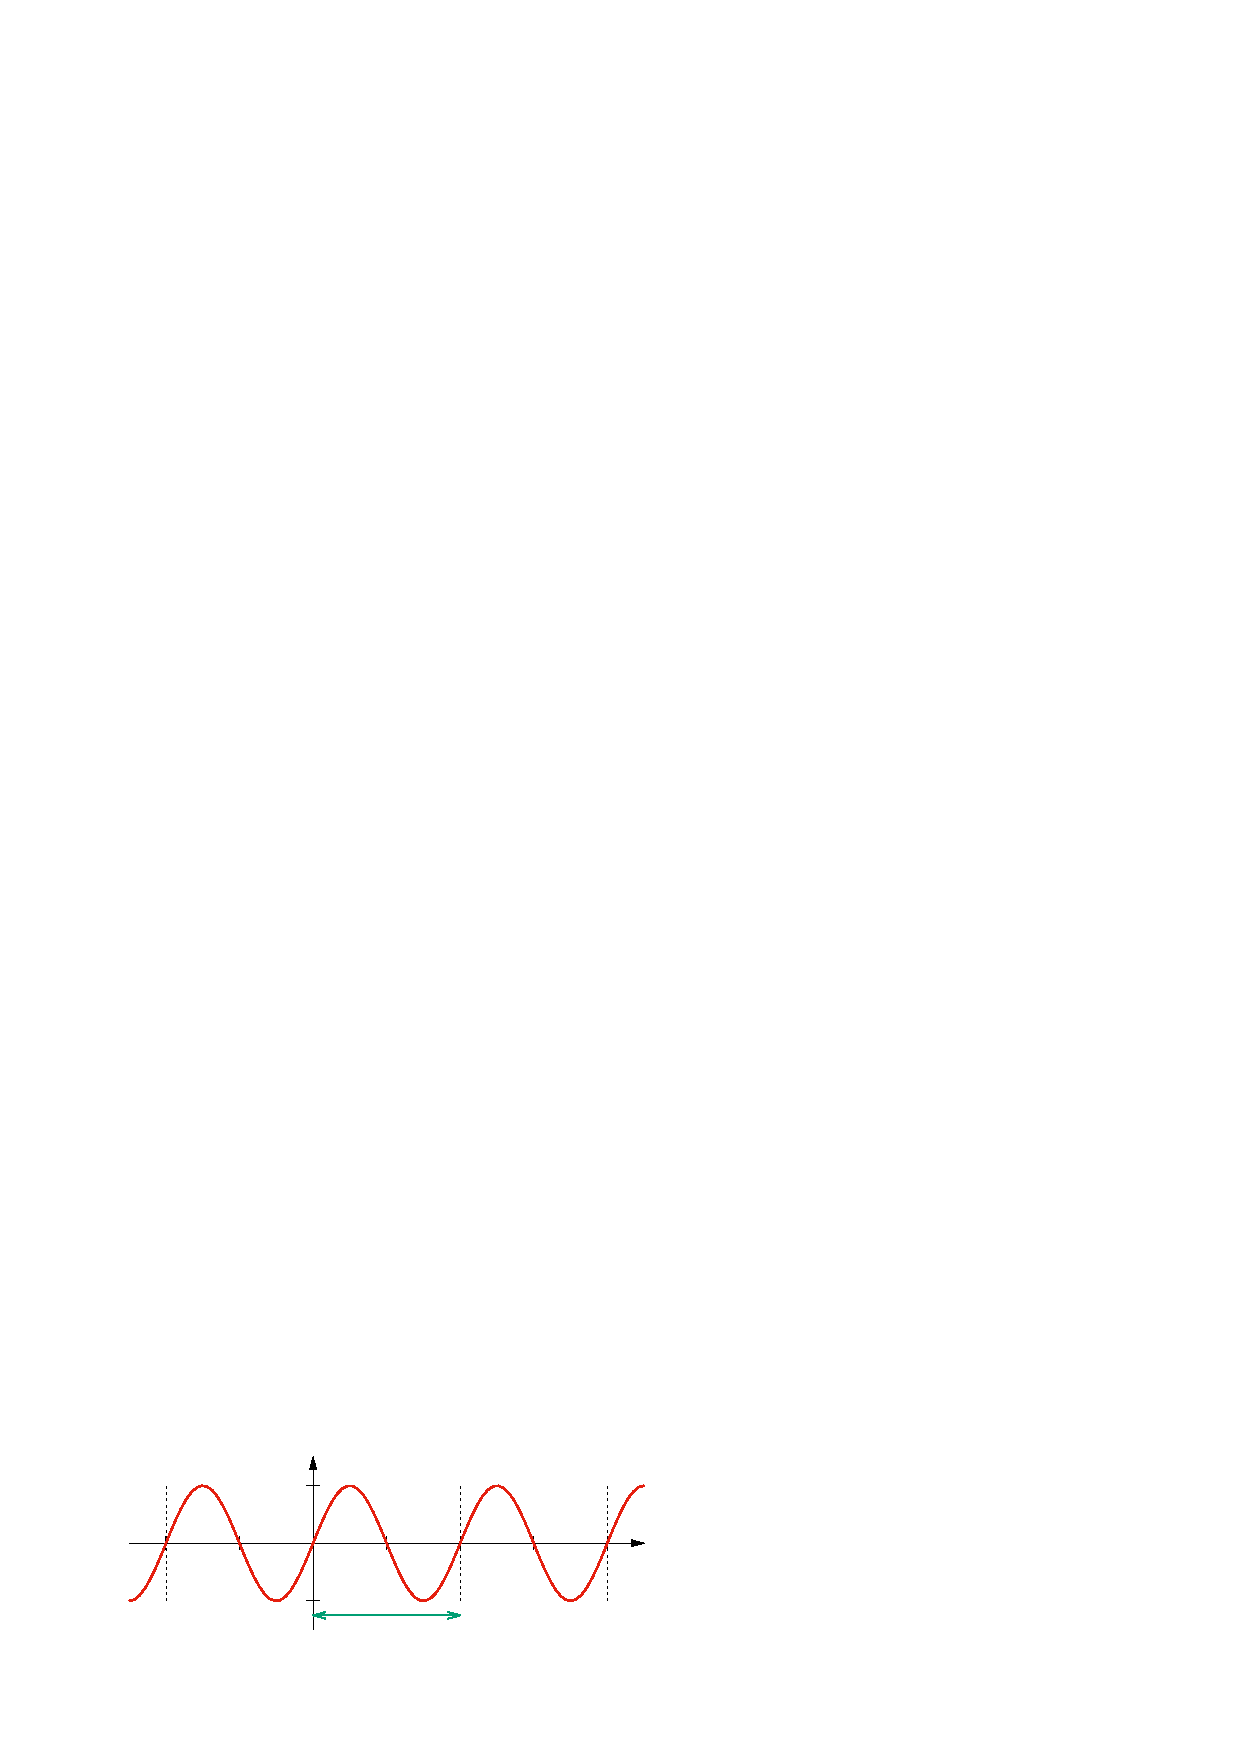
\includegraphics[width={273.60bp},height={100.70bp}]{figura_01_01}}%
    \gplfronttext
  \end{picture}%
\endgroup

    \caption{Función periódica}\label{figura_01}
\end{figure}

Una función periódica es aquella cuya gráfica se repite infinitas veces, cada
cierto intervalo (\textbf{Figura~\ref{figura_01}}).

El menor intervalo de repetición se llama \emph{periodo} ($T$).

Matemáticamente una función periódica es aquella que verifica:
\begin{equation}
    f(t)=f(t+nT);n\in\mathbb{Z}
\label{funcion_periodica}
\end{equation}

Donde $T$ es el periodo (la menor constante que verifica la igualdad).

\section{Propiedades de la funciones periódicas}
Si $f(t)=f(t+nT)$:
\subsection*{Propiedad 1}
\begin{equation}
    \int_a^b\,f(t)\,dt=\int_{a+nT}^{b+nT}f(t)\,dt\quad\,n\in\mathbb{Z}
\label{propiedad1}
\end{equation}

\underline{Prueba}:
\begin{equation*}
    \int_a^b\,f(t)\,dt=\int_{a}^{b}\,f(t+nT)\,dt
\end{equation*}

Cambiando la variable:
\begin{equation*}
    \tau=t+nT
\end{equation*}
\begin{equation*}
    d\tau=dt
\end{equation*}
\begin{equation*}
\begin{split}
    \int_a^b\,f(t)\,dt
        &=\int_{a+nT}^{b+nT}\,f(\tau)\,d\tau\\
        &=\int_{a+nT}^{b+nT}\,f(t)\,dt
\end{split}
\end{equation*}

Puede verse gráficamente en la \textbf{Figura~\ref{figura_02}}.
\begin{figure}[H]
    \centering
    % GNUPLOT: LaTeX picture with Postscript
\begingroup
  \makeatletter
  \providecommand\color[2][]{%
    \GenericError{(gnuplot) \space\space\space\@spaces}{%
      Package color not loaded in conjunction with
      terminal option `colourtext'%
    }{See the gnuplot documentation for explanation.%
    }{Either use 'blacktext' in gnuplot or load the package
      color.sty in LaTeX.}%
    \renewcommand\color[2][]{}%
  }%
  \providecommand\includegraphics[2][]{%
    \GenericError{(gnuplot) \space\space\space\@spaces}{%
      Package graphicx or graphics not loaded%
    }{See the gnuplot documentation for explanation.%
    }{The gnuplot epslatex terminal needs graphicx.sty or graphics.sty.}%
    \renewcommand\includegraphics[2][]{}%
  }%
  \providecommand\rotatebox[2]{#2}%
  \@ifundefined{ifGPcolor}{%
    \newif\ifGPcolor
    \GPcolorfalse
  }{}%
  \@ifundefined{ifGPblacktext}{%
    \newif\ifGPblacktext
    \GPblacktexttrue
  }{}%
  % define a \g@addto@macro without @ in the name:
  \let\gplgaddtomacro\g@addto@macro
  % define empty templates for all commands taking text:
  \gdef\gplbacktext{}%
  \gdef\gplfronttext{}%
  \makeatother
  \ifGPblacktext
    % no textcolor at all
    \def\colorrgb#1{}%
    \def\colorgray#1{}%
  \else
    % gray or color?
    \ifGPcolor
      \def\colorrgb#1{\color[rgb]{#1}}%
      \def\colorgray#1{\color[gray]{#1}}%
      \expandafter\def\csname LTw\endcsname{\color{white}}%
      \expandafter\def\csname LTb\endcsname{\color{black}}%
      \expandafter\def\csname LTa\endcsname{\color{black}}%
      \expandafter\def\csname LT0\endcsname{\color[rgb]{1,0,0}}%
      \expandafter\def\csname LT1\endcsname{\color[rgb]{0,1,0}}%
      \expandafter\def\csname LT2\endcsname{\color[rgb]{0,0,1}}%
      \expandafter\def\csname LT3\endcsname{\color[rgb]{1,0,1}}%
      \expandafter\def\csname LT4\endcsname{\color[rgb]{0,1,1}}%
      \expandafter\def\csname LT5\endcsname{\color[rgb]{1,1,0}}%
      \expandafter\def\csname LT6\endcsname{\color[rgb]{0,0,0}}%
      \expandafter\def\csname LT7\endcsname{\color[rgb]{1,0.3,0}}%
      \expandafter\def\csname LT8\endcsname{\color[rgb]{0.5,0.5,0.5}}%
    \else
      % gray
      \def\colorrgb#1{\color{black}}%
      \def\colorgray#1{\color[gray]{#1}}%
      \expandafter\def\csname LTw\endcsname{\color{white}}%
      \expandafter\def\csname LTb\endcsname{\color{black}}%
      \expandafter\def\csname LTa\endcsname{\color{black}}%
      \expandafter\def\csname LT0\endcsname{\color{black}}%
      \expandafter\def\csname LT1\endcsname{\color{black}}%
      \expandafter\def\csname LT2\endcsname{\color{black}}%
      \expandafter\def\csname LT3\endcsname{\color{black}}%
      \expandafter\def\csname LT4\endcsname{\color{black}}%
      \expandafter\def\csname LT5\endcsname{\color{black}}%
      \expandafter\def\csname LT6\endcsname{\color{black}}%
      \expandafter\def\csname LT7\endcsname{\color{black}}%
      \expandafter\def\csname LT8\endcsname{\color{black}}%
    \fi
  \fi
    \setlength{\unitlength}{0.0500bp}%
    \ifx\gptboxheight\undefined%
      \newlength{\gptboxheight}%
      \newlength{\gptboxwidth}%
      \newsavebox{\gptboxtext}%
    \fi%
    \setlength{\fboxrule}{0.5pt}%
    \setlength{\fboxsep}{1pt}%
    \definecolor{tbcol}{rgb}{1,1,1}%
\begin{picture}(6336.00,2590.00)%
    \gplgaddtomacro\gplbacktext{%
      \csname LTb\endcsname%%
      \put(1233,416){\makebox(0,0)[r]{\strut{}}}%
      \put(1233,863){\makebox(0,0)[r]{\strut{}}}%
      \put(1233,1311){\makebox(0,0)[r]{\strut{}}}%
      \put(1233,1758){\makebox(0,0)[r]{\strut{}}}%
      \put(1233,2205){\makebox(0,0)[r]{\strut{}}}%
      \put(603,640){\makebox(0,0){\strut{}}}%
      \put(1329,640){\makebox(0,0){\strut{}}}%
      \put(2055,640){\makebox(0,0){\strut{}}}%
      \put(2781,640){\makebox(0,0){\strut{}}}%
      \put(3506,640){\makebox(0,0){\strut{}}}%
      \put(4232,640){\makebox(0,0){\strut{}}}%
      \put(4958,640){\makebox(0,0){\strut{}}}%
      \put(5684,640){\makebox(0,0){\strut{}}}%
      \csname LTb\endcsname%%
      \put(6228,863){\makebox(0,0)[l]{\strut{}$t$}}%
      \put(1502,2429){\makebox(0,0)[l]{\strut{}$f(t)$}}%
      \put(2020,662){\makebox(0,0)[l]{\strut{}$a$}}%
      \put(2746,662){\makebox(0,0)[l]{\strut{}$b$}}%
      \put(3955,662){\makebox(0,0)[l]{\strut{}$a+T$}}%
      \put(4704,662){\makebox(0,0)[l]{\strut{}$b+T$}}%
      \put(1766,1982){\makebox(0,0)[l]{\strut{}$\int_a^b f(t) dt$}}%
      \put(3943,2295){\makebox(0,0)[l]{\strut{}$\int_{a+T}^{b+T} f(t+T) dt$}}%
    }%
    \gplgaddtomacro\gplfronttext{%
    }%
    \gplgaddtomacro\gplbacktext{%
      \csname LTb\endcsname%%
      \put(1233,416){\makebox(0,0)[r]{\strut{}}}%
      \put(1233,863){\makebox(0,0)[r]{\strut{}}}%
      \put(1233,1311){\makebox(0,0)[r]{\strut{}}}%
      \put(1233,1758){\makebox(0,0)[r]{\strut{}}}%
      \put(1233,2205){\makebox(0,0)[r]{\strut{}}}%
      \put(603,640){\makebox(0,0){\strut{}}}%
      \put(1329,640){\makebox(0,0){\strut{}}}%
      \put(2055,640){\makebox(0,0){\strut{}}}%
      \put(2781,640){\makebox(0,0){\strut{}}}%
      \put(3506,640){\makebox(0,0){\strut{}}}%
      \put(4232,640){\makebox(0,0){\strut{}}}%
      \put(4958,640){\makebox(0,0){\strut{}}}%
      \put(5684,640){\makebox(0,0){\strut{}}}%
      \csname LTb\endcsname%%
      \put(6228,863){\makebox(0,0)[l]{\strut{}$t$}}%
      \put(1502,2429){\makebox(0,0)[l]{\strut{}$f(t)$}}%
      \put(2020,662){\makebox(0,0)[l]{\strut{}$a$}}%
      \put(2746,662){\makebox(0,0)[l]{\strut{}$b$}}%
      \put(3955,662){\makebox(0,0)[l]{\strut{}$a+T$}}%
      \put(4704,662){\makebox(0,0)[l]{\strut{}$b+T$}}%
      \put(1766,1982){\makebox(0,0)[l]{\strut{}$\int_a^b f(t) dt$}}%
      \put(3943,2295){\makebox(0,0)[l]{\strut{}$\int_{a+T}^{b+T} f(t+T) dt$}}%
    }%
    \gplgaddtomacro\gplfronttext{%
    }%
    \gplgaddtomacro\gplbacktext{%
      \csname LTb\endcsname%%
      \put(1233,416){\makebox(0,0)[r]{\strut{}}}%
      \put(1233,863){\makebox(0,0)[r]{\strut{}}}%
      \put(1233,1311){\makebox(0,0)[r]{\strut{}}}%
      \put(1233,1758){\makebox(0,0)[r]{\strut{}}}%
      \put(1233,2205){\makebox(0,0)[r]{\strut{}}}%
      \put(603,640){\makebox(0,0){\strut{}}}%
      \put(1329,640){\makebox(0,0){\strut{}}}%
      \put(2055,640){\makebox(0,0){\strut{}}}%
      \put(2781,640){\makebox(0,0){\strut{}}}%
      \put(3506,640){\makebox(0,0){\strut{}}}%
      \put(4232,640){\makebox(0,0){\strut{}}}%
      \put(4958,640){\makebox(0,0){\strut{}}}%
      \put(5684,640){\makebox(0,0){\strut{}}}%
      \csname LTb\endcsname%%
      \put(6228,863){\makebox(0,0)[l]{\strut{}$t$}}%
      \put(1502,2429){\makebox(0,0)[l]{\strut{}$f(t)$}}%
      \put(2020,662){\makebox(0,0)[l]{\strut{}$a$}}%
      \put(2746,662){\makebox(0,0)[l]{\strut{}$b$}}%
      \put(3955,662){\makebox(0,0)[l]{\strut{}$a+T$}}%
      \put(4704,662){\makebox(0,0)[l]{\strut{}$b+T$}}%
      \put(1766,1982){\makebox(0,0)[l]{\strut{}$\int_a^b f(t) dt$}}%
      \put(3943,2295){\makebox(0,0)[l]{\strut{}$\int_{a+T}^{b+T} f(t+T) dt$}}%
    }%
    \gplgaddtomacro\gplfronttext{%
    }%
    \gplgaddtomacro\gplbacktext{%
      \csname LTb\endcsname%%
      \put(1233,416){\makebox(0,0)[r]{\strut{}}}%
      \put(1233,863){\makebox(0,0)[r]{\strut{}}}%
      \put(1233,1311){\makebox(0,0)[r]{\strut{}}}%
      \put(1233,1758){\makebox(0,0)[r]{\strut{}}}%
      \put(1233,2205){\makebox(0,0)[r]{\strut{}}}%
      \put(603,640){\makebox(0,0){\strut{}}}%
      \put(1329,640){\makebox(0,0){\strut{}}}%
      \put(2055,640){\makebox(0,0){\strut{}}}%
      \put(2781,640){\makebox(0,0){\strut{}}}%
      \put(3506,640){\makebox(0,0){\strut{}}}%
      \put(4232,640){\makebox(0,0){\strut{}}}%
      \put(4958,640){\makebox(0,0){\strut{}}}%
      \put(5684,640){\makebox(0,0){\strut{}}}%
      \csname LTb\endcsname%%
      \put(6228,863){\makebox(0,0)[l]{\strut{}$t$}}%
      \put(1502,2429){\makebox(0,0)[l]{\strut{}$f(t)$}}%
      \put(2020,662){\makebox(0,0)[l]{\strut{}$a$}}%
      \put(2746,662){\makebox(0,0)[l]{\strut{}$b$}}%
      \put(3955,662){\makebox(0,0)[l]{\strut{}$a+T$}}%
      \put(4704,662){\makebox(0,0)[l]{\strut{}$b+T$}}%
      \put(1766,1982){\makebox(0,0)[l]{\strut{}$\int_a^b f(t) dt$}}%
      \put(3943,2295){\makebox(0,0)[l]{\strut{}$\int_{a+T}^{b+T} f(t+T) dt$}}%
    }%
    \gplgaddtomacro\gplfronttext{%
    }%
    \gplgaddtomacro\gplbacktext{%
      \csname LTb\endcsname%%
      \put(1233,416){\makebox(0,0)[r]{\strut{}}}%
      \put(1233,863){\makebox(0,0)[r]{\strut{}}}%
      \put(1233,1311){\makebox(0,0)[r]{\strut{}}}%
      \put(1233,1758){\makebox(0,0)[r]{\strut{}}}%
      \put(1233,2205){\makebox(0,0)[r]{\strut{}}}%
      \put(603,640){\makebox(0,0){\strut{}}}%
      \put(1329,640){\makebox(0,0){\strut{}}}%
      \put(2055,640){\makebox(0,0){\strut{}}}%
      \put(2781,640){\makebox(0,0){\strut{}}}%
      \put(3506,640){\makebox(0,0){\strut{}}}%
      \put(4232,640){\makebox(0,0){\strut{}}}%
      \put(4958,640){\makebox(0,0){\strut{}}}%
      \put(5684,640){\makebox(0,0){\strut{}}}%
      \csname LTb\endcsname%%
      \put(6228,863){\makebox(0,0)[l]{\strut{}$t$}}%
      \put(1502,2429){\makebox(0,0)[l]{\strut{}$f(t)$}}%
      \put(2020,662){\makebox(0,0)[l]{\strut{}$a$}}%
      \put(2746,662){\makebox(0,0)[l]{\strut{}$b$}}%
      \put(3955,662){\makebox(0,0)[l]{\strut{}$a+T$}}%
      \put(4704,662){\makebox(0,0)[l]{\strut{}$b+T$}}%
      \put(1766,1982){\makebox(0,0)[l]{\strut{}$\int_a^b f(t) dt$}}%
      \put(3943,2295){\makebox(0,0)[l]{\strut{}$\int_{a+T}^{b+T} f(t+T) dt$}}%
    }%
    \gplgaddtomacro\gplfronttext{%
    }%
    \gplgaddtomacro\gplbacktext{%
      \csname LTb\endcsname%%
      \put(1233,416){\makebox(0,0)[r]{\strut{}}}%
      \put(1233,863){\makebox(0,0)[r]{\strut{}}}%
      \put(1233,1311){\makebox(0,0)[r]{\strut{}}}%
      \put(1233,1758){\makebox(0,0)[r]{\strut{}}}%
      \put(1233,2205){\makebox(0,0)[r]{\strut{}}}%
      \put(603,640){\makebox(0,0){\strut{}}}%
      \put(1329,640){\makebox(0,0){\strut{}}}%
      \put(2055,640){\makebox(0,0){\strut{}}}%
      \put(2781,640){\makebox(0,0){\strut{}}}%
      \put(3506,640){\makebox(0,0){\strut{}}}%
      \put(4232,640){\makebox(0,0){\strut{}}}%
      \put(4958,640){\makebox(0,0){\strut{}}}%
      \put(5684,640){\makebox(0,0){\strut{}}}%
      \csname LTb\endcsname%%
      \put(6228,863){\makebox(0,0)[l]{\strut{}$t$}}%
      \put(1502,2429){\makebox(0,0)[l]{\strut{}$f(t)$}}%
      \put(2020,662){\makebox(0,0)[l]{\strut{}$a$}}%
      \put(2746,662){\makebox(0,0)[l]{\strut{}$b$}}%
      \put(3955,662){\makebox(0,0)[l]{\strut{}$a+T$}}%
      \put(4704,662){\makebox(0,0)[l]{\strut{}$b+T$}}%
      \put(1766,1982){\makebox(0,0)[l]{\strut{}$\int_a^b f(t) dt$}}%
      \put(3943,2295){\makebox(0,0)[l]{\strut{}$\int_{a+T}^{b+T} f(t+T) dt$}}%
    }%
    \gplgaddtomacro\gplfronttext{%
    }%
    \gplbacktext
    \put(0,0){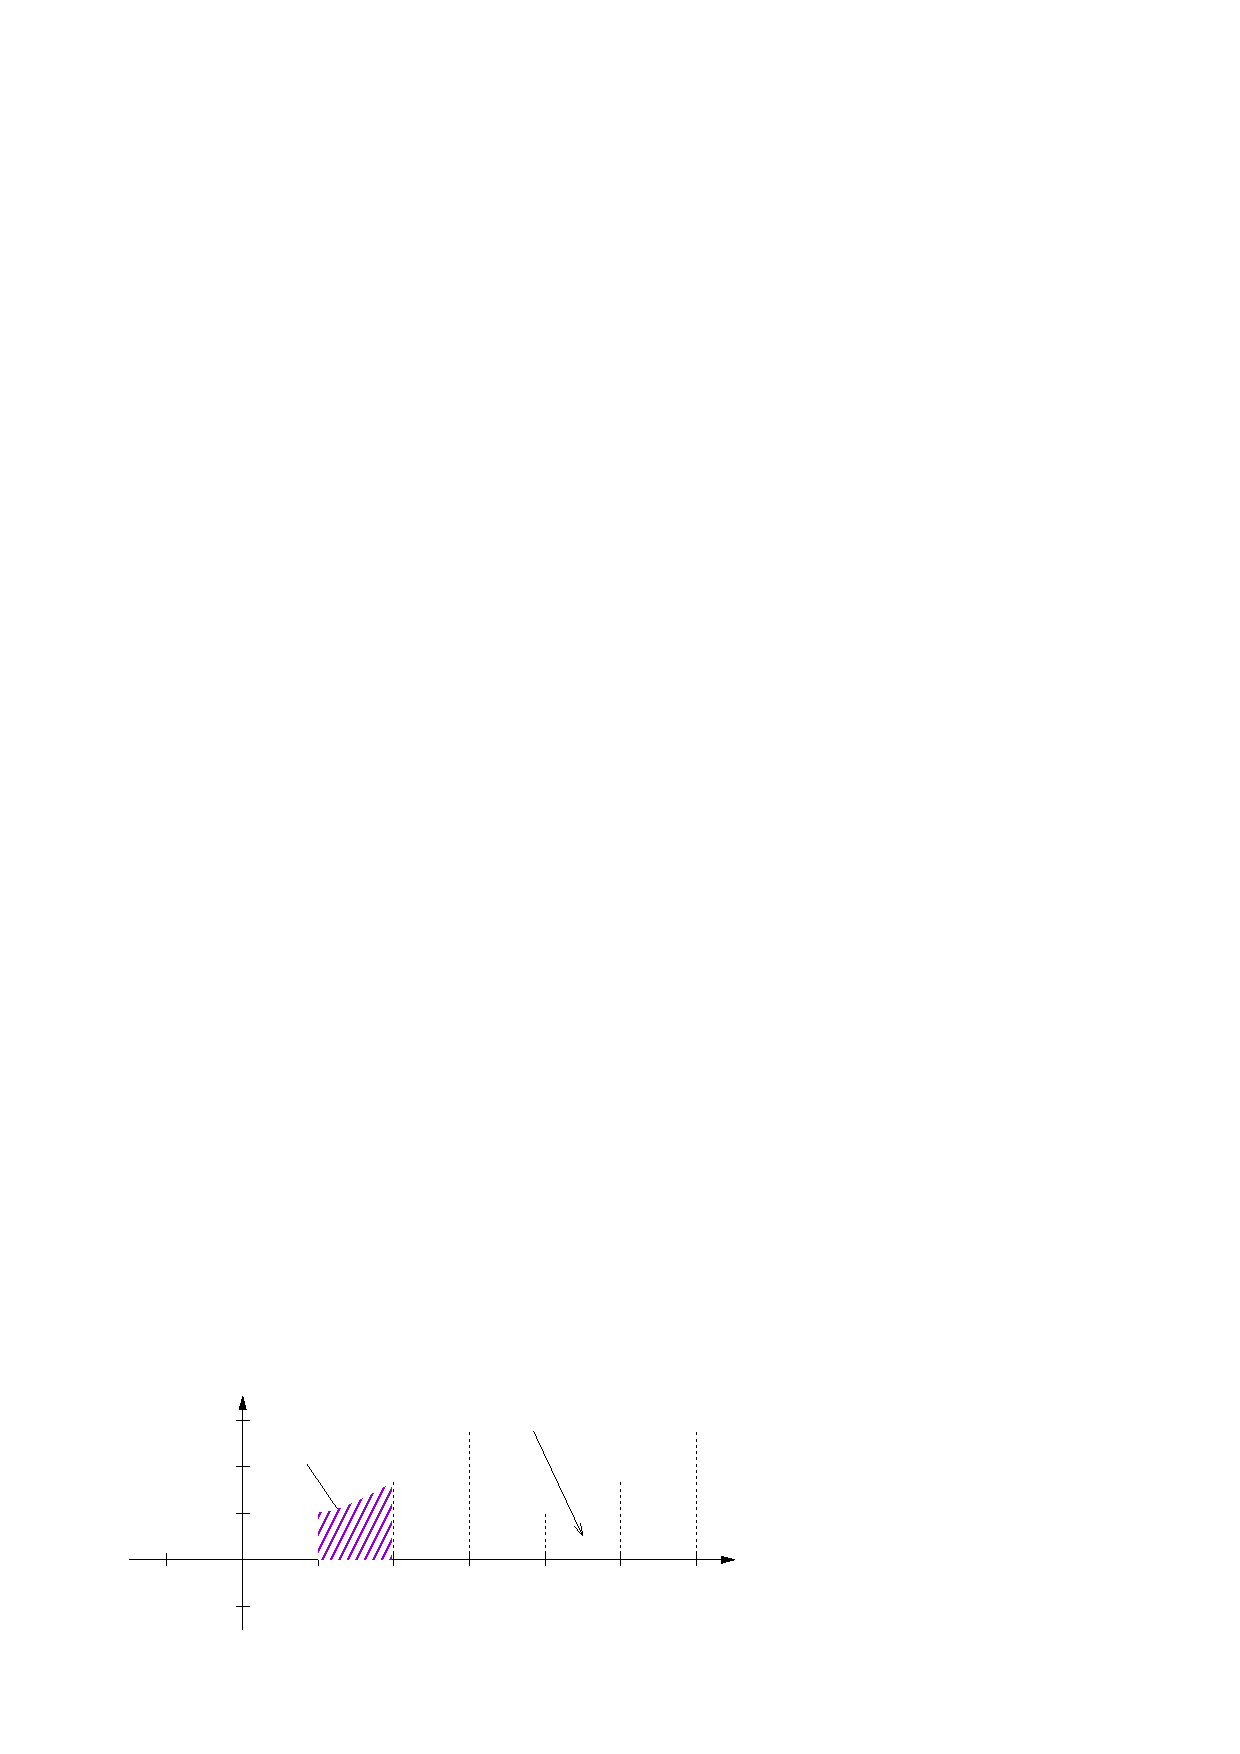
\includegraphics[width={316.80bp},height={129.50bp}]{figura_01_02}}%
    \gplfronttext
  \end{picture}%
\endgroup

    \caption{Demostración gráfica}\label{figura_02}
\end{figure}

\subsection*{Propiedad 2}
\begin{equation}
    \int_{a-T/2}^{a+T/2}f(t)\,dt=\int_{-T/2}^{T/2}f(t)\,dt
\label{propiedad2}
\end{equation}

\underline{Prueba}:
\begin{equation*}
\begin{split}
    \int_{a-T/2}^{a+T/2}f(t)\,dt
        &=\int_{a-T/2}^{T/2}f(t)\,dt+\int_{T/2}^{a+T/2}f(t)\,dt\\
        &=\int_{a-T/2}^{T/2}f(t)\,dt+\int_{T/2-T}^{a+T/2-T}f(t)\,dt\\
        &=\int_{a-T/2}^{T/2}f(t)\,dt+\int_{-T/2}^{a-T/2}f(t)\,dt\\
        &=\int_{-T/2}^{T/2}f(t)\,dt
\end{split}
\end{equation*}

Puede verse gráficamente en la \textbf{Figura~\ref{figura_03}}.
\begin{figure}[H]
    \centering
    % GNUPLOT: LaTeX picture with Postscript
\begingroup
  \makeatletter
  \providecommand\color[2][]{%
    \GenericError{(gnuplot) \space\space\space\@spaces}{%
      Package color not loaded in conjunction with
      terminal option `colourtext'%
    }{See the gnuplot documentation for explanation.%
    }{Either use 'blacktext' in gnuplot or load the package
      color.sty in LaTeX.}%
    \renewcommand\color[2][]{}%
  }%
  \providecommand\includegraphics[2][]{%
    \GenericError{(gnuplot) \space\space\space\@spaces}{%
      Package graphicx or graphics not loaded%
    }{See the gnuplot documentation for explanation.%
    }{The gnuplot epslatex terminal needs graphicx.sty or graphics.sty.}%
    \renewcommand\includegraphics[2][]{}%
  }%
  \providecommand\rotatebox[2]{#2}%
  \@ifundefined{ifGPcolor}{%
    \newif\ifGPcolor
    \GPcolorfalse
  }{}%
  \@ifundefined{ifGPblacktext}{%
    \newif\ifGPblacktext
    \GPblacktexttrue
  }{}%
  % define a \g@addto@macro without @ in the name:
  \let\gplgaddtomacro\g@addto@macro
  % define empty templates for all commands taking text:
  \gdef\gplbacktext{}%
  \gdef\gplfronttext{}%
  \makeatother
  \ifGPblacktext
    % no textcolor at all
    \def\colorrgb#1{}%
    \def\colorgray#1{}%
  \else
    % gray or color?
    \ifGPcolor
      \def\colorrgb#1{\color[rgb]{#1}}%
      \def\colorgray#1{\color[gray]{#1}}%
      \expandafter\def\csname LTw\endcsname{\color{white}}%
      \expandafter\def\csname LTb\endcsname{\color{black}}%
      \expandafter\def\csname LTa\endcsname{\color{black}}%
      \expandafter\def\csname LT0\endcsname{\color[rgb]{1,0,0}}%
      \expandafter\def\csname LT1\endcsname{\color[rgb]{0,1,0}}%
      \expandafter\def\csname LT2\endcsname{\color[rgb]{0,0,1}}%
      \expandafter\def\csname LT3\endcsname{\color[rgb]{1,0,1}}%
      \expandafter\def\csname LT4\endcsname{\color[rgb]{0,1,1}}%
      \expandafter\def\csname LT5\endcsname{\color[rgb]{1,1,0}}%
      \expandafter\def\csname LT6\endcsname{\color[rgb]{0,0,0}}%
      \expandafter\def\csname LT7\endcsname{\color[rgb]{1,0.3,0}}%
      \expandafter\def\csname LT8\endcsname{\color[rgb]{0.5,0.5,0.5}}%
    \else
      % gray
      \def\colorrgb#1{\color{black}}%
      \def\colorgray#1{\color[gray]{#1}}%
      \expandafter\def\csname LTw\endcsname{\color{white}}%
      \expandafter\def\csname LTb\endcsname{\color{black}}%
      \expandafter\def\csname LTa\endcsname{\color{black}}%
      \expandafter\def\csname LT0\endcsname{\color{black}}%
      \expandafter\def\csname LT1\endcsname{\color{black}}%
      \expandafter\def\csname LT2\endcsname{\color{black}}%
      \expandafter\def\csname LT3\endcsname{\color{black}}%
      \expandafter\def\csname LT4\endcsname{\color{black}}%
      \expandafter\def\csname LT5\endcsname{\color{black}}%
      \expandafter\def\csname LT6\endcsname{\color{black}}%
      \expandafter\def\csname LT7\endcsname{\color{black}}%
      \expandafter\def\csname LT8\endcsname{\color{black}}%
    \fi
  \fi
    \setlength{\unitlength}{0.0500bp}%
    \ifx\gptboxheight\undefined%
      \newlength{\gptboxheight}%
      \newlength{\gptboxwidth}%
      \newsavebox{\gptboxtext}%
    \fi%
    \setlength{\fboxrule}{0.5pt}%
    \setlength{\fboxsep}{1pt}%
    \definecolor{tbcol}{rgb}{1,1,1}%
\begin{picture}(6336.00,2590.00)%
    \gplgaddtomacro\gplbacktext{%
      \csname LTb\endcsname%%
      \put(1757,416){\makebox(0,0)[r]{\strut{}}}%
      \put(1757,863){\makebox(0,0)[r]{\strut{}}}%
      \put(1757,1311){\makebox(0,0)[r]{\strut{}}}%
      \put(1757,1758){\makebox(0,0)[r]{\strut{}}}%
      \put(1757,2205){\makebox(0,0)[r]{\strut{}}}%
      \put(563,640){\makebox(0,0){\strut{}}}%
      \put(1208,640){\makebox(0,0){\strut{}}}%
      \put(1853,640){\makebox(0,0){\strut{}}}%
      \put(2498,640){\makebox(0,0){\strut{}}}%
      \put(3143,640){\makebox(0,0){\strut{}}}%
      \put(3789,640){\makebox(0,0){\strut{}}}%
      \put(4434,640){\makebox(0,0){\strut{}}}%
      \put(5079,640){\makebox(0,0){\strut{}}}%
      \put(5724,640){\makebox(0,0){\strut{}}}%
      \csname LTb\endcsname%%
      \put(6208,863){\makebox(0,0)[l]{\strut{}$t$}}%
      \put(2007,2429){\makebox(0,0)[l]{\strut{}$f(t)$}}%
      \put(631,662){\makebox(0,0)[l]{\strut{}$-\frac{T}{2}$}}%
      \put(2728,662){\makebox(0,0)[l]{\strut{}$\frac{T}{2}$}}%
      \put(3203,662){\makebox(0,0)[l]{\strut{}$a-\frac{T}{2}$}}%
      \put(4383,662){\makebox(0,0)[l]{\strut{}$a$}}%
      \put(5201,662){\makebox(0,0)[l]{\strut{}$a+\frac{T}{2}$}}%
      \put(306,2026){\makebox(0,0)[l]{\strut{}$\int_{-\frac{T}{2}}^{\frac{T}{2}} f(t) dt$}}%
      \put(4177,2295){\makebox(0,0)[l]{\strut{}$\int_{a-\frac{T}{2}}^{a+\frac{T}{2}} f(t) dt$}}%
    }%
    \gplgaddtomacro\gplfronttext{%
    }%
    \gplgaddtomacro\gplbacktext{%
      \csname LTb\endcsname%%
      \put(1757,416){\makebox(0,0)[r]{\strut{}}}%
      \put(1757,863){\makebox(0,0)[r]{\strut{}}}%
      \put(1757,1311){\makebox(0,0)[r]{\strut{}}}%
      \put(1757,1758){\makebox(0,0)[r]{\strut{}}}%
      \put(1757,2205){\makebox(0,0)[r]{\strut{}}}%
      \put(563,640){\makebox(0,0){\strut{}}}%
      \put(1208,640){\makebox(0,0){\strut{}}}%
      \put(1853,640){\makebox(0,0){\strut{}}}%
      \put(2498,640){\makebox(0,0){\strut{}}}%
      \put(3143,640){\makebox(0,0){\strut{}}}%
      \put(3789,640){\makebox(0,0){\strut{}}}%
      \put(4434,640){\makebox(0,0){\strut{}}}%
      \put(5079,640){\makebox(0,0){\strut{}}}%
      \put(5724,640){\makebox(0,0){\strut{}}}%
      \csname LTb\endcsname%%
      \put(6208,863){\makebox(0,0)[l]{\strut{}$t$}}%
      \put(2007,2429){\makebox(0,0)[l]{\strut{}$f(t)$}}%
      \put(631,662){\makebox(0,0)[l]{\strut{}$-\frac{T}{2}$}}%
      \put(2728,662){\makebox(0,0)[l]{\strut{}$\frac{T}{2}$}}%
      \put(3203,662){\makebox(0,0)[l]{\strut{}$a-\frac{T}{2}$}}%
      \put(4383,662){\makebox(0,0)[l]{\strut{}$a$}}%
      \put(5201,662){\makebox(0,0)[l]{\strut{}$a+\frac{T}{2}$}}%
      \put(306,2026){\makebox(0,0)[l]{\strut{}$\int_{-\frac{T}{2}}^{\frac{T}{2}} f(t) dt$}}%
      \put(4177,2295){\makebox(0,0)[l]{\strut{}$\int_{a-\frac{T}{2}}^{a+\frac{T}{2}} f(t) dt$}}%
    }%
    \gplgaddtomacro\gplfronttext{%
    }%
    \gplgaddtomacro\gplbacktext{%
      \csname LTb\endcsname%%
      \put(1757,416){\makebox(0,0)[r]{\strut{}}}%
      \put(1757,863){\makebox(0,0)[r]{\strut{}}}%
      \put(1757,1311){\makebox(0,0)[r]{\strut{}}}%
      \put(1757,1758){\makebox(0,0)[r]{\strut{}}}%
      \put(1757,2205){\makebox(0,0)[r]{\strut{}}}%
      \put(563,640){\makebox(0,0){\strut{}}}%
      \put(1208,640){\makebox(0,0){\strut{}}}%
      \put(1853,640){\makebox(0,0){\strut{}}}%
      \put(2498,640){\makebox(0,0){\strut{}}}%
      \put(3143,640){\makebox(0,0){\strut{}}}%
      \put(3789,640){\makebox(0,0){\strut{}}}%
      \put(4434,640){\makebox(0,0){\strut{}}}%
      \put(5079,640){\makebox(0,0){\strut{}}}%
      \put(5724,640){\makebox(0,0){\strut{}}}%
      \csname LTb\endcsname%%
      \put(6208,863){\makebox(0,0)[l]{\strut{}$t$}}%
      \put(2007,2429){\makebox(0,0)[l]{\strut{}$f(t)$}}%
      \put(631,662){\makebox(0,0)[l]{\strut{}$-\frac{T}{2}$}}%
      \put(2728,662){\makebox(0,0)[l]{\strut{}$\frac{T}{2}$}}%
      \put(3203,662){\makebox(0,0)[l]{\strut{}$a-\frac{T}{2}$}}%
      \put(4383,662){\makebox(0,0)[l]{\strut{}$a$}}%
      \put(5201,662){\makebox(0,0)[l]{\strut{}$a+\frac{T}{2}$}}%
      \put(306,2026){\makebox(0,0)[l]{\strut{}$\int_{-\frac{T}{2}}^{\frac{T}{2}} f(t) dt$}}%
      \put(4177,2295){\makebox(0,0)[l]{\strut{}$\int_{a-\frac{T}{2}}^{a+\frac{T}{2}} f(t) dt$}}%
    }%
    \gplgaddtomacro\gplfronttext{%
    }%
    \gplgaddtomacro\gplbacktext{%
      \csname LTb\endcsname%%
      \put(1757,416){\makebox(0,0)[r]{\strut{}}}%
      \put(1757,863){\makebox(0,0)[r]{\strut{}}}%
      \put(1757,1311){\makebox(0,0)[r]{\strut{}}}%
      \put(1757,1758){\makebox(0,0)[r]{\strut{}}}%
      \put(1757,2205){\makebox(0,0)[r]{\strut{}}}%
      \put(563,640){\makebox(0,0){\strut{}}}%
      \put(1208,640){\makebox(0,0){\strut{}}}%
      \put(1853,640){\makebox(0,0){\strut{}}}%
      \put(2498,640){\makebox(0,0){\strut{}}}%
      \put(3143,640){\makebox(0,0){\strut{}}}%
      \put(3789,640){\makebox(0,0){\strut{}}}%
      \put(4434,640){\makebox(0,0){\strut{}}}%
      \put(5079,640){\makebox(0,0){\strut{}}}%
      \put(5724,640){\makebox(0,0){\strut{}}}%
      \csname LTb\endcsname%%
      \put(6208,863){\makebox(0,0)[l]{\strut{}$t$}}%
      \put(2007,2429){\makebox(0,0)[l]{\strut{}$f(t)$}}%
      \put(631,662){\makebox(0,0)[l]{\strut{}$-\frac{T}{2}$}}%
      \put(2728,662){\makebox(0,0)[l]{\strut{}$\frac{T}{2}$}}%
      \put(3203,662){\makebox(0,0)[l]{\strut{}$a-\frac{T}{2}$}}%
      \put(4383,662){\makebox(0,0)[l]{\strut{}$a$}}%
      \put(5201,662){\makebox(0,0)[l]{\strut{}$a+\frac{T}{2}$}}%
      \put(306,2026){\makebox(0,0)[l]{\strut{}$\int_{-\frac{T}{2}}^{\frac{T}{2}} f(t) dt$}}%
      \put(4177,2295){\makebox(0,0)[l]{\strut{}$\int_{a-\frac{T}{2}}^{a+\frac{T}{2}} f(t) dt$}}%
    }%
    \gplgaddtomacro\gplfronttext{%
    }%
    \gplgaddtomacro\gplbacktext{%
      \csname LTb\endcsname%%
      \put(1757,416){\makebox(0,0)[r]{\strut{}}}%
      \put(1757,863){\makebox(0,0)[r]{\strut{}}}%
      \put(1757,1311){\makebox(0,0)[r]{\strut{}}}%
      \put(1757,1758){\makebox(0,0)[r]{\strut{}}}%
      \put(1757,2205){\makebox(0,0)[r]{\strut{}}}%
      \put(563,640){\makebox(0,0){\strut{}}}%
      \put(1208,640){\makebox(0,0){\strut{}}}%
      \put(1853,640){\makebox(0,0){\strut{}}}%
      \put(2498,640){\makebox(0,0){\strut{}}}%
      \put(3143,640){\makebox(0,0){\strut{}}}%
      \put(3789,640){\makebox(0,0){\strut{}}}%
      \put(4434,640){\makebox(0,0){\strut{}}}%
      \put(5079,640){\makebox(0,0){\strut{}}}%
      \put(5724,640){\makebox(0,0){\strut{}}}%
      \csname LTb\endcsname%%
      \put(6208,863){\makebox(0,0)[l]{\strut{}$t$}}%
      \put(2007,2429){\makebox(0,0)[l]{\strut{}$f(t)$}}%
      \put(631,662){\makebox(0,0)[l]{\strut{}$-\frac{T}{2}$}}%
      \put(2728,662){\makebox(0,0)[l]{\strut{}$\frac{T}{2}$}}%
      \put(3203,662){\makebox(0,0)[l]{\strut{}$a-\frac{T}{2}$}}%
      \put(4383,662){\makebox(0,0)[l]{\strut{}$a$}}%
      \put(5201,662){\makebox(0,0)[l]{\strut{}$a+\frac{T}{2}$}}%
      \put(306,2026){\makebox(0,0)[l]{\strut{}$\int_{-\frac{T}{2}}^{\frac{T}{2}} f(t) dt$}}%
      \put(4177,2295){\makebox(0,0)[l]{\strut{}$\int_{a-\frac{T}{2}}^{a+\frac{T}{2}} f(t) dt$}}%
    }%
    \gplgaddtomacro\gplfronttext{%
    }%
    \gplgaddtomacro\gplbacktext{%
      \csname LTb\endcsname%%
      \put(1757,416){\makebox(0,0)[r]{\strut{}}}%
      \put(1757,863){\makebox(0,0)[r]{\strut{}}}%
      \put(1757,1311){\makebox(0,0)[r]{\strut{}}}%
      \put(1757,1758){\makebox(0,0)[r]{\strut{}}}%
      \put(1757,2205){\makebox(0,0)[r]{\strut{}}}%
      \put(563,640){\makebox(0,0){\strut{}}}%
      \put(1208,640){\makebox(0,0){\strut{}}}%
      \put(1853,640){\makebox(0,0){\strut{}}}%
      \put(2498,640){\makebox(0,0){\strut{}}}%
      \put(3143,640){\makebox(0,0){\strut{}}}%
      \put(3789,640){\makebox(0,0){\strut{}}}%
      \put(4434,640){\makebox(0,0){\strut{}}}%
      \put(5079,640){\makebox(0,0){\strut{}}}%
      \put(5724,640){\makebox(0,0){\strut{}}}%
      \csname LTb\endcsname%%
      \put(6208,863){\makebox(0,0)[l]{\strut{}$t$}}%
      \put(2007,2429){\makebox(0,0)[l]{\strut{}$f(t)$}}%
      \put(631,662){\makebox(0,0)[l]{\strut{}$-\frac{T}{2}$}}%
      \put(2728,662){\makebox(0,0)[l]{\strut{}$\frac{T}{2}$}}%
      \put(3203,662){\makebox(0,0)[l]{\strut{}$a-\frac{T}{2}$}}%
      \put(4383,662){\makebox(0,0)[l]{\strut{}$a$}}%
      \put(5201,662){\makebox(0,0)[l]{\strut{}$a+\frac{T}{2}$}}%
      \put(306,2026){\makebox(0,0)[l]{\strut{}$\int_{-\frac{T}{2}}^{\frac{T}{2}} f(t) dt$}}%
      \put(4177,2295){\makebox(0,0)[l]{\strut{}$\int_{a-\frac{T}{2}}^{a+\frac{T}{2}} f(t) dt$}}%
    }%
    \gplgaddtomacro\gplfronttext{%
    }%
    \gplgaddtomacro\gplbacktext{%
      \csname LTb\endcsname%%
      \put(1757,416){\makebox(0,0)[r]{\strut{}}}%
      \put(1757,863){\makebox(0,0)[r]{\strut{}}}%
      \put(1757,1311){\makebox(0,0)[r]{\strut{}}}%
      \put(1757,1758){\makebox(0,0)[r]{\strut{}}}%
      \put(1757,2205){\makebox(0,0)[r]{\strut{}}}%
      \put(563,640){\makebox(0,0){\strut{}}}%
      \put(1208,640){\makebox(0,0){\strut{}}}%
      \put(1853,640){\makebox(0,0){\strut{}}}%
      \put(2498,640){\makebox(0,0){\strut{}}}%
      \put(3143,640){\makebox(0,0){\strut{}}}%
      \put(3789,640){\makebox(0,0){\strut{}}}%
      \put(4434,640){\makebox(0,0){\strut{}}}%
      \put(5079,640){\makebox(0,0){\strut{}}}%
      \put(5724,640){\makebox(0,0){\strut{}}}%
      \csname LTb\endcsname%%
      \put(6208,863){\makebox(0,0)[l]{\strut{}$t$}}%
      \put(2007,2429){\makebox(0,0)[l]{\strut{}$f(t)$}}%
      \put(631,662){\makebox(0,0)[l]{\strut{}$-\frac{T}{2}$}}%
      \put(2728,662){\makebox(0,0)[l]{\strut{}$\frac{T}{2}$}}%
      \put(3203,662){\makebox(0,0)[l]{\strut{}$a-\frac{T}{2}$}}%
      \put(4383,662){\makebox(0,0)[l]{\strut{}$a$}}%
      \put(5201,662){\makebox(0,0)[l]{\strut{}$a+\frac{T}{2}$}}%
      \put(306,2026){\makebox(0,0)[l]{\strut{}$\int_{-\frac{T}{2}}^{\frac{T}{2}} f(t) dt$}}%
      \put(4177,2295){\makebox(0,0)[l]{\strut{}$\int_{a-\frac{T}{2}}^{a+\frac{T}{2}} f(t) dt$}}%
    }%
    \gplgaddtomacro\gplfronttext{%
    }%
    \gplgaddtomacro\gplbacktext{%
      \csname LTb\endcsname%%
      \put(1757,416){\makebox(0,0)[r]{\strut{}}}%
      \put(1757,863){\makebox(0,0)[r]{\strut{}}}%
      \put(1757,1311){\makebox(0,0)[r]{\strut{}}}%
      \put(1757,1758){\makebox(0,0)[r]{\strut{}}}%
      \put(1757,2205){\makebox(0,0)[r]{\strut{}}}%
      \put(563,640){\makebox(0,0){\strut{}}}%
      \put(1208,640){\makebox(0,0){\strut{}}}%
      \put(1853,640){\makebox(0,0){\strut{}}}%
      \put(2498,640){\makebox(0,0){\strut{}}}%
      \put(3143,640){\makebox(0,0){\strut{}}}%
      \put(3789,640){\makebox(0,0){\strut{}}}%
      \put(4434,640){\makebox(0,0){\strut{}}}%
      \put(5079,640){\makebox(0,0){\strut{}}}%
      \put(5724,640){\makebox(0,0){\strut{}}}%
      \csname LTb\endcsname%%
      \put(6208,863){\makebox(0,0)[l]{\strut{}$t$}}%
      \put(2007,2429){\makebox(0,0)[l]{\strut{}$f(t)$}}%
      \put(631,662){\makebox(0,0)[l]{\strut{}$-\frac{T}{2}$}}%
      \put(2728,662){\makebox(0,0)[l]{\strut{}$\frac{T}{2}$}}%
      \put(3203,662){\makebox(0,0)[l]{\strut{}$a-\frac{T}{2}$}}%
      \put(4383,662){\makebox(0,0)[l]{\strut{}$a$}}%
      \put(5201,662){\makebox(0,0)[l]{\strut{}$a+\frac{T}{2}$}}%
      \put(306,2026){\makebox(0,0)[l]{\strut{}$\int_{-\frac{T}{2}}^{\frac{T}{2}} f(t) dt$}}%
      \put(4177,2295){\makebox(0,0)[l]{\strut{}$\int_{a-\frac{T}{2}}^{a+\frac{T}{2}} f(t) dt$}}%
    }%
    \gplgaddtomacro\gplfronttext{%
    }%
    \gplbacktext
    \put(0,0){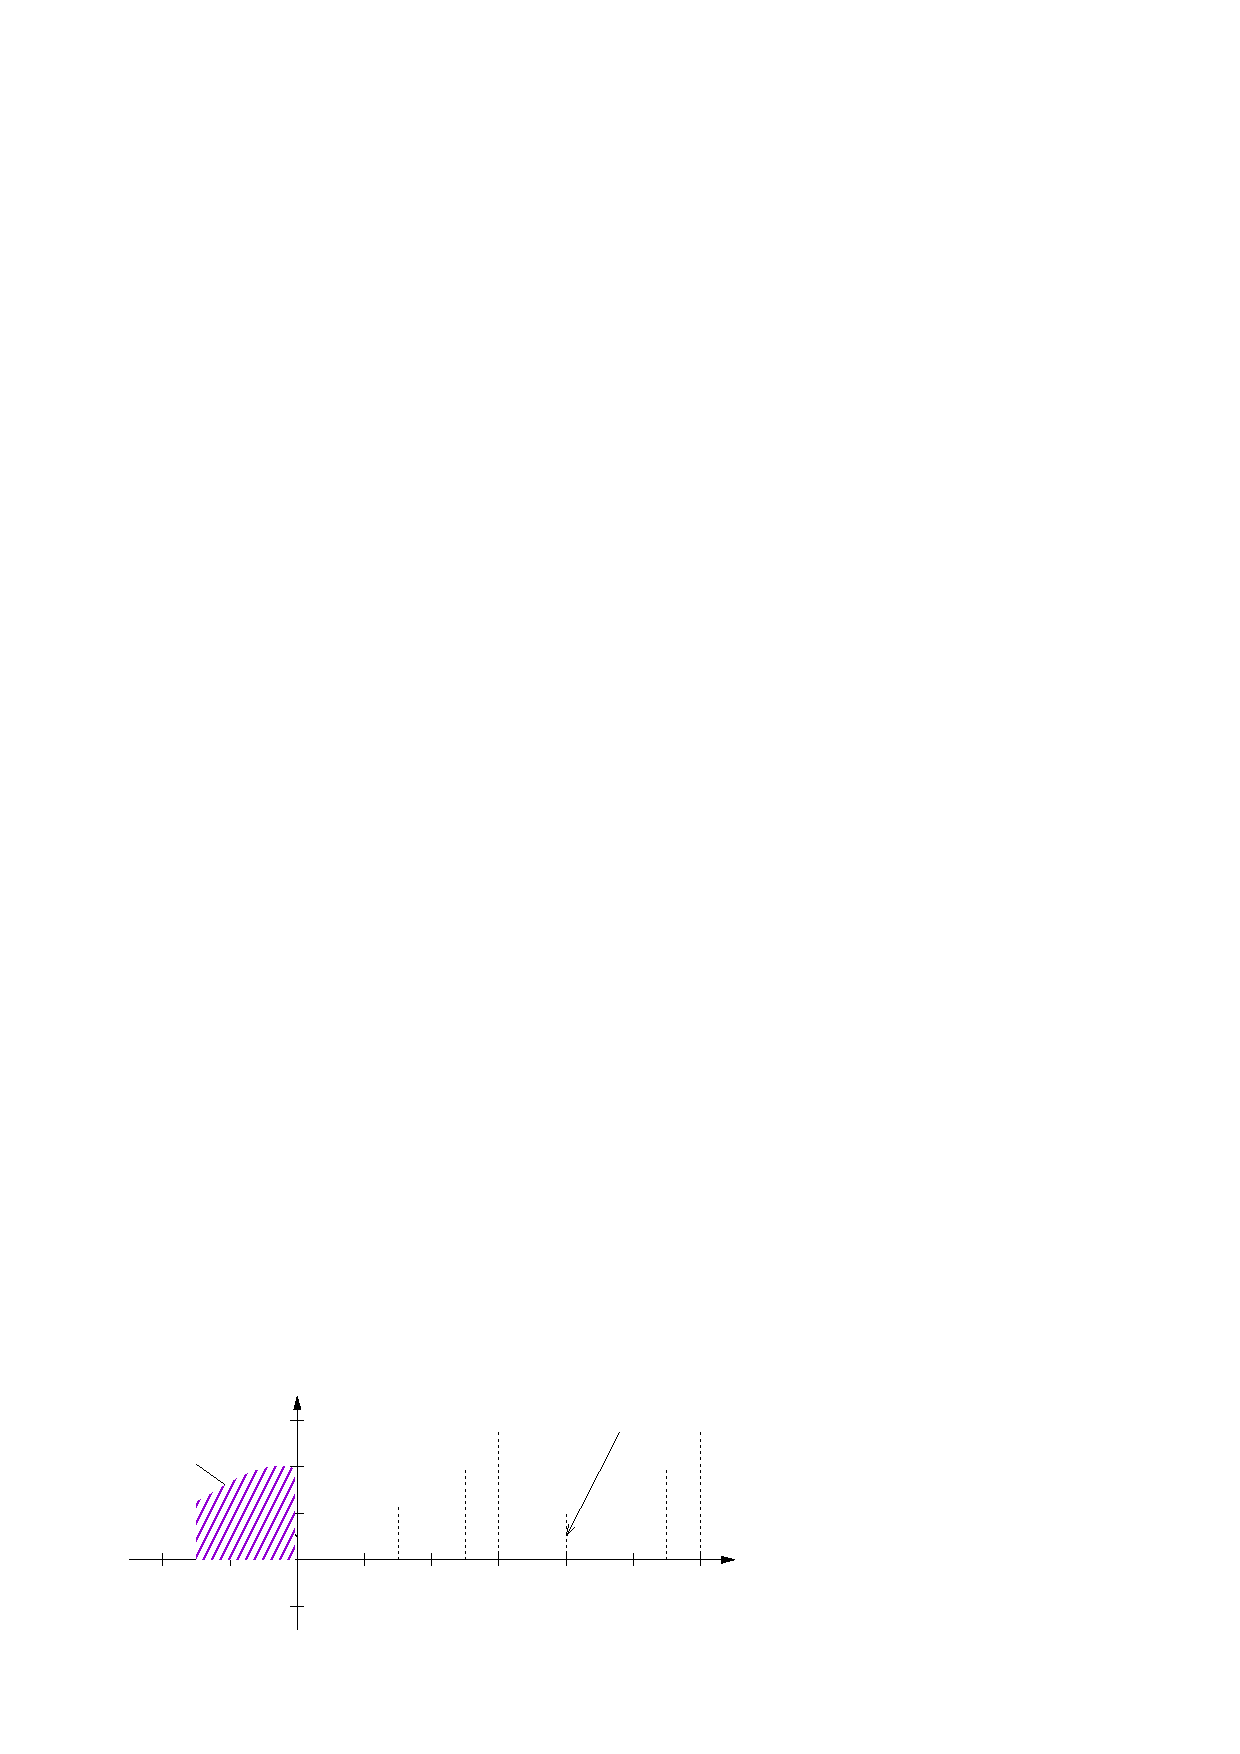
\includegraphics[width={316.80bp},height={129.50bp}]{figura_01_03}}%
    \gplfronttext
  \end{picture}%
\endgroup

    \caption{Demostración gráfica}\label{figura_03}
\end{figure}

\subsection*{Propiedad 3}
\begin{equation}
    \int_{0}^{T}f(t)\,dt=\int_{-T/2}^{T/2}f(t)\,dt
\label{propiedad3}
\end{equation}

\underline{Prueba}:

Si en la ecuación (\ref{propiedad2}) $a=T/2$:
\begin{equation*}
\begin{split}
    \int_{-T/2}^{T/2}f(t)\,dt
        &=\int_{a-T/2}^{a+T/2}f(t)\,dt\\
        &=\int_{T/2-T/2}^{T/2+T/2}f(t)\,dt\\
        &=\int_{0}^{T}f(t)\,dt
\end{split}
\end{equation*}

Puede verse gráficamente en la \textbf{Figura~\ref{figura_04}}.
\begin{figure}[H]
    \centering
    % GNUPLOT: LaTeX picture with Postscript
\begingroup
  \makeatletter
  \providecommand\color[2][]{%
    \GenericError{(gnuplot) \space\space\space\@spaces}{%
      Package color not loaded in conjunction with
      terminal option `colourtext'%
    }{See the gnuplot documentation for explanation.%
    }{Either use 'blacktext' in gnuplot or load the package
      color.sty in LaTeX.}%
    \renewcommand\color[2][]{}%
  }%
  \providecommand\includegraphics[2][]{%
    \GenericError{(gnuplot) \space\space\space\@spaces}{%
      Package graphicx or graphics not loaded%
    }{See the gnuplot documentation for explanation.%
    }{The gnuplot epslatex terminal needs graphicx.sty or graphics.sty.}%
    \renewcommand\includegraphics[2][]{}%
  }%
  \providecommand\rotatebox[2]{#2}%
  \@ifundefined{ifGPcolor}{%
    \newif\ifGPcolor
    \GPcolorfalse
  }{}%
  \@ifundefined{ifGPblacktext}{%
    \newif\ifGPblacktext
    \GPblacktexttrue
  }{}%
  % define a \g@addto@macro without @ in the name:
  \let\gplgaddtomacro\g@addto@macro
  % define empty templates for all commands taking text:
  \gdef\gplbacktext{}%
  \gdef\gplfronttext{}%
  \makeatother
  \ifGPblacktext
    % no textcolor at all
    \def\colorrgb#1{}%
    \def\colorgray#1{}%
  \else
    % gray or color?
    \ifGPcolor
      \def\colorrgb#1{\color[rgb]{#1}}%
      \def\colorgray#1{\color[gray]{#1}}%
      \expandafter\def\csname LTw\endcsname{\color{white}}%
      \expandafter\def\csname LTb\endcsname{\color{black}}%
      \expandafter\def\csname LTa\endcsname{\color{black}}%
      \expandafter\def\csname LT0\endcsname{\color[rgb]{1,0,0}}%
      \expandafter\def\csname LT1\endcsname{\color[rgb]{0,1,0}}%
      \expandafter\def\csname LT2\endcsname{\color[rgb]{0,0,1}}%
      \expandafter\def\csname LT3\endcsname{\color[rgb]{1,0,1}}%
      \expandafter\def\csname LT4\endcsname{\color[rgb]{0,1,1}}%
      \expandafter\def\csname LT5\endcsname{\color[rgb]{1,1,0}}%
      \expandafter\def\csname LT6\endcsname{\color[rgb]{0,0,0}}%
      \expandafter\def\csname LT7\endcsname{\color[rgb]{1,0.3,0}}%
      \expandafter\def\csname LT8\endcsname{\color[rgb]{0.5,0.5,0.5}}%
    \else
      % gray
      \def\colorrgb#1{\color{black}}%
      \def\colorgray#1{\color[gray]{#1}}%
      \expandafter\def\csname LTw\endcsname{\color{white}}%
      \expandafter\def\csname LTb\endcsname{\color{black}}%
      \expandafter\def\csname LTa\endcsname{\color{black}}%
      \expandafter\def\csname LT0\endcsname{\color{black}}%
      \expandafter\def\csname LT1\endcsname{\color{black}}%
      \expandafter\def\csname LT2\endcsname{\color{black}}%
      \expandafter\def\csname LT3\endcsname{\color{black}}%
      \expandafter\def\csname LT4\endcsname{\color{black}}%
      \expandafter\def\csname LT5\endcsname{\color{black}}%
      \expandafter\def\csname LT6\endcsname{\color{black}}%
      \expandafter\def\csname LT7\endcsname{\color{black}}%
      \expandafter\def\csname LT8\endcsname{\color{black}}%
    \fi
  \fi
    \setlength{\unitlength}{0.0500bp}%
    \ifx\gptboxheight\undefined%
      \newlength{\gptboxheight}%
      \newlength{\gptboxwidth}%
      \newsavebox{\gptboxtext}%
    \fi%
    \setlength{\fboxrule}{0.5pt}%
    \setlength{\fboxsep}{1pt}%
    \definecolor{tbcol}{rgb}{1,1,1}%
\begin{picture}(6336.00,2590.00)%
    \gplgaddtomacro\gplbacktext{%
      \csname LTb\endcsname%%
      \put(2356,455){\makebox(0,0)[r]{\strut{}}}%
      \put(2356,982){\makebox(0,0)[r]{\strut{}}}%
      \put(2356,1508){\makebox(0,0)[r]{\strut{}}}%
      \put(2356,2034){\makebox(0,0)[r]{\strut{}}}%
      \put(240,759){\makebox(0,0){\strut{}}}%
      \put(1346,759){\makebox(0,0){\strut{}}}%
      \put(2452,759){\makebox(0,0){\strut{}}}%
      \put(3558,759){\makebox(0,0){\strut{}}}%
      \put(4664,759){\makebox(0,0){\strut{}}}%
      \put(5770,759){\makebox(0,0){\strut{}}}%
      \csname LTb\endcsname%%
      \put(6324,982){\makebox(0,0)[l]{\strut{}$t$}}%
      \put(2628,2561){\makebox(0,0)[l]{\strut{}$f(t)$}}%
      \put(574,745){\makebox(0,0)[l]{\strut{}$-\frac{T}{2}$}}%
      \put(4059,745){\makebox(0,0)[l]{\strut{}$ \frac{T}{2}$}}%
      \put(5735,745){\makebox(0,0)[l]{\strut{}$T$}}%
      \put(265,2350){\makebox(0,0)[l]{\strut{}$\int_{-\frac{T}{2}}^{\frac{T}{2}} f(t) dt$}}%
      \put(3231,2350){\makebox(0,0)[l]{\strut{}$\int_{0}^{T} f(t) dt$}}%
    }%
    \gplgaddtomacro\gplfronttext{%
    }%
    \gplgaddtomacro\gplbacktext{%
      \csname LTb\endcsname%%
      \put(2356,455){\makebox(0,0)[r]{\strut{}}}%
      \put(2356,982){\makebox(0,0)[r]{\strut{}}}%
      \put(2356,1508){\makebox(0,0)[r]{\strut{}}}%
      \put(2356,2034){\makebox(0,0)[r]{\strut{}}}%
      \put(240,759){\makebox(0,0){\strut{}}}%
      \put(1346,759){\makebox(0,0){\strut{}}}%
      \put(2452,759){\makebox(0,0){\strut{}}}%
      \put(3558,759){\makebox(0,0){\strut{}}}%
      \put(4664,759){\makebox(0,0){\strut{}}}%
      \put(5770,759){\makebox(0,0){\strut{}}}%
      \csname LTb\endcsname%%
      \put(6324,982){\makebox(0,0)[l]{\strut{}$t$}}%
      \put(2628,2561){\makebox(0,0)[l]{\strut{}$f(t)$}}%
      \put(574,745){\makebox(0,0)[l]{\strut{}$-\frac{T}{2}$}}%
      \put(4059,745){\makebox(0,0)[l]{\strut{}$ \frac{T}{2}$}}%
      \put(5735,745){\makebox(0,0)[l]{\strut{}$T$}}%
      \put(265,2350){\makebox(0,0)[l]{\strut{}$\int_{-\frac{T}{2}}^{\frac{T}{2}} f(t) dt$}}%
      \put(3231,2350){\makebox(0,0)[l]{\strut{}$\int_{0}^{T} f(t) dt$}}%
    }%
    \gplgaddtomacro\gplfronttext{%
    }%
    \gplgaddtomacro\gplbacktext{%
      \csname LTb\endcsname%%
      \put(2356,455){\makebox(0,0)[r]{\strut{}}}%
      \put(2356,982){\makebox(0,0)[r]{\strut{}}}%
      \put(2356,1508){\makebox(0,0)[r]{\strut{}}}%
      \put(2356,2034){\makebox(0,0)[r]{\strut{}}}%
      \put(240,759){\makebox(0,0){\strut{}}}%
      \put(1346,759){\makebox(0,0){\strut{}}}%
      \put(2452,759){\makebox(0,0){\strut{}}}%
      \put(3558,759){\makebox(0,0){\strut{}}}%
      \put(4664,759){\makebox(0,0){\strut{}}}%
      \put(5770,759){\makebox(0,0){\strut{}}}%
      \csname LTb\endcsname%%
      \put(6324,982){\makebox(0,0)[l]{\strut{}$t$}}%
      \put(2628,2561){\makebox(0,0)[l]{\strut{}$f(t)$}}%
      \put(574,745){\makebox(0,0)[l]{\strut{}$-\frac{T}{2}$}}%
      \put(4059,745){\makebox(0,0)[l]{\strut{}$ \frac{T}{2}$}}%
      \put(5735,745){\makebox(0,0)[l]{\strut{}$T$}}%
      \put(265,2350){\makebox(0,0)[l]{\strut{}$\int_{-\frac{T}{2}}^{\frac{T}{2}} f(t) dt$}}%
      \put(3231,2350){\makebox(0,0)[l]{\strut{}$\int_{0}^{T} f(t) dt$}}%
    }%
    \gplgaddtomacro\gplfronttext{%
    }%
    \gplgaddtomacro\gplbacktext{%
      \csname LTb\endcsname%%
      \put(2356,455){\makebox(0,0)[r]{\strut{}}}%
      \put(2356,982){\makebox(0,0)[r]{\strut{}}}%
      \put(2356,1508){\makebox(0,0)[r]{\strut{}}}%
      \put(2356,2034){\makebox(0,0)[r]{\strut{}}}%
      \put(240,759){\makebox(0,0){\strut{}}}%
      \put(1346,759){\makebox(0,0){\strut{}}}%
      \put(2452,759){\makebox(0,0){\strut{}}}%
      \put(3558,759){\makebox(0,0){\strut{}}}%
      \put(4664,759){\makebox(0,0){\strut{}}}%
      \put(5770,759){\makebox(0,0){\strut{}}}%
      \csname LTb\endcsname%%
      \put(6324,982){\makebox(0,0)[l]{\strut{}$t$}}%
      \put(2628,2561){\makebox(0,0)[l]{\strut{}$f(t)$}}%
      \put(574,745){\makebox(0,0)[l]{\strut{}$-\frac{T}{2}$}}%
      \put(4059,745){\makebox(0,0)[l]{\strut{}$ \frac{T}{2}$}}%
      \put(5735,745){\makebox(0,0)[l]{\strut{}$T$}}%
      \put(265,2350){\makebox(0,0)[l]{\strut{}$\int_{-\frac{T}{2}}^{\frac{T}{2}} f(t) dt$}}%
      \put(3231,2350){\makebox(0,0)[l]{\strut{}$\int_{0}^{T} f(t) dt$}}%
    }%
    \gplgaddtomacro\gplfronttext{%
    }%
    \gplgaddtomacro\gplbacktext{%
      \csname LTb\endcsname%%
      \put(2356,455){\makebox(0,0)[r]{\strut{}}}%
      \put(2356,982){\makebox(0,0)[r]{\strut{}}}%
      \put(2356,1508){\makebox(0,0)[r]{\strut{}}}%
      \put(2356,2034){\makebox(0,0)[r]{\strut{}}}%
      \put(240,759){\makebox(0,0){\strut{}}}%
      \put(1346,759){\makebox(0,0){\strut{}}}%
      \put(2452,759){\makebox(0,0){\strut{}}}%
      \put(3558,759){\makebox(0,0){\strut{}}}%
      \put(4664,759){\makebox(0,0){\strut{}}}%
      \put(5770,759){\makebox(0,0){\strut{}}}%
      \csname LTb\endcsname%%
      \put(6324,982){\makebox(0,0)[l]{\strut{}$t$}}%
      \put(2628,2561){\makebox(0,0)[l]{\strut{}$f(t)$}}%
      \put(574,745){\makebox(0,0)[l]{\strut{}$-\frac{T}{2}$}}%
      \put(4059,745){\makebox(0,0)[l]{\strut{}$ \frac{T}{2}$}}%
      \put(5735,745){\makebox(0,0)[l]{\strut{}$T$}}%
      \put(265,2350){\makebox(0,0)[l]{\strut{}$\int_{-\frac{T}{2}}^{\frac{T}{2}} f(t) dt$}}%
      \put(3231,2350){\makebox(0,0)[l]{\strut{}$\int_{0}^{T} f(t) dt$}}%
    }%
    \gplgaddtomacro\gplfronttext{%
    }%
    \gplbacktext
    \put(0,0){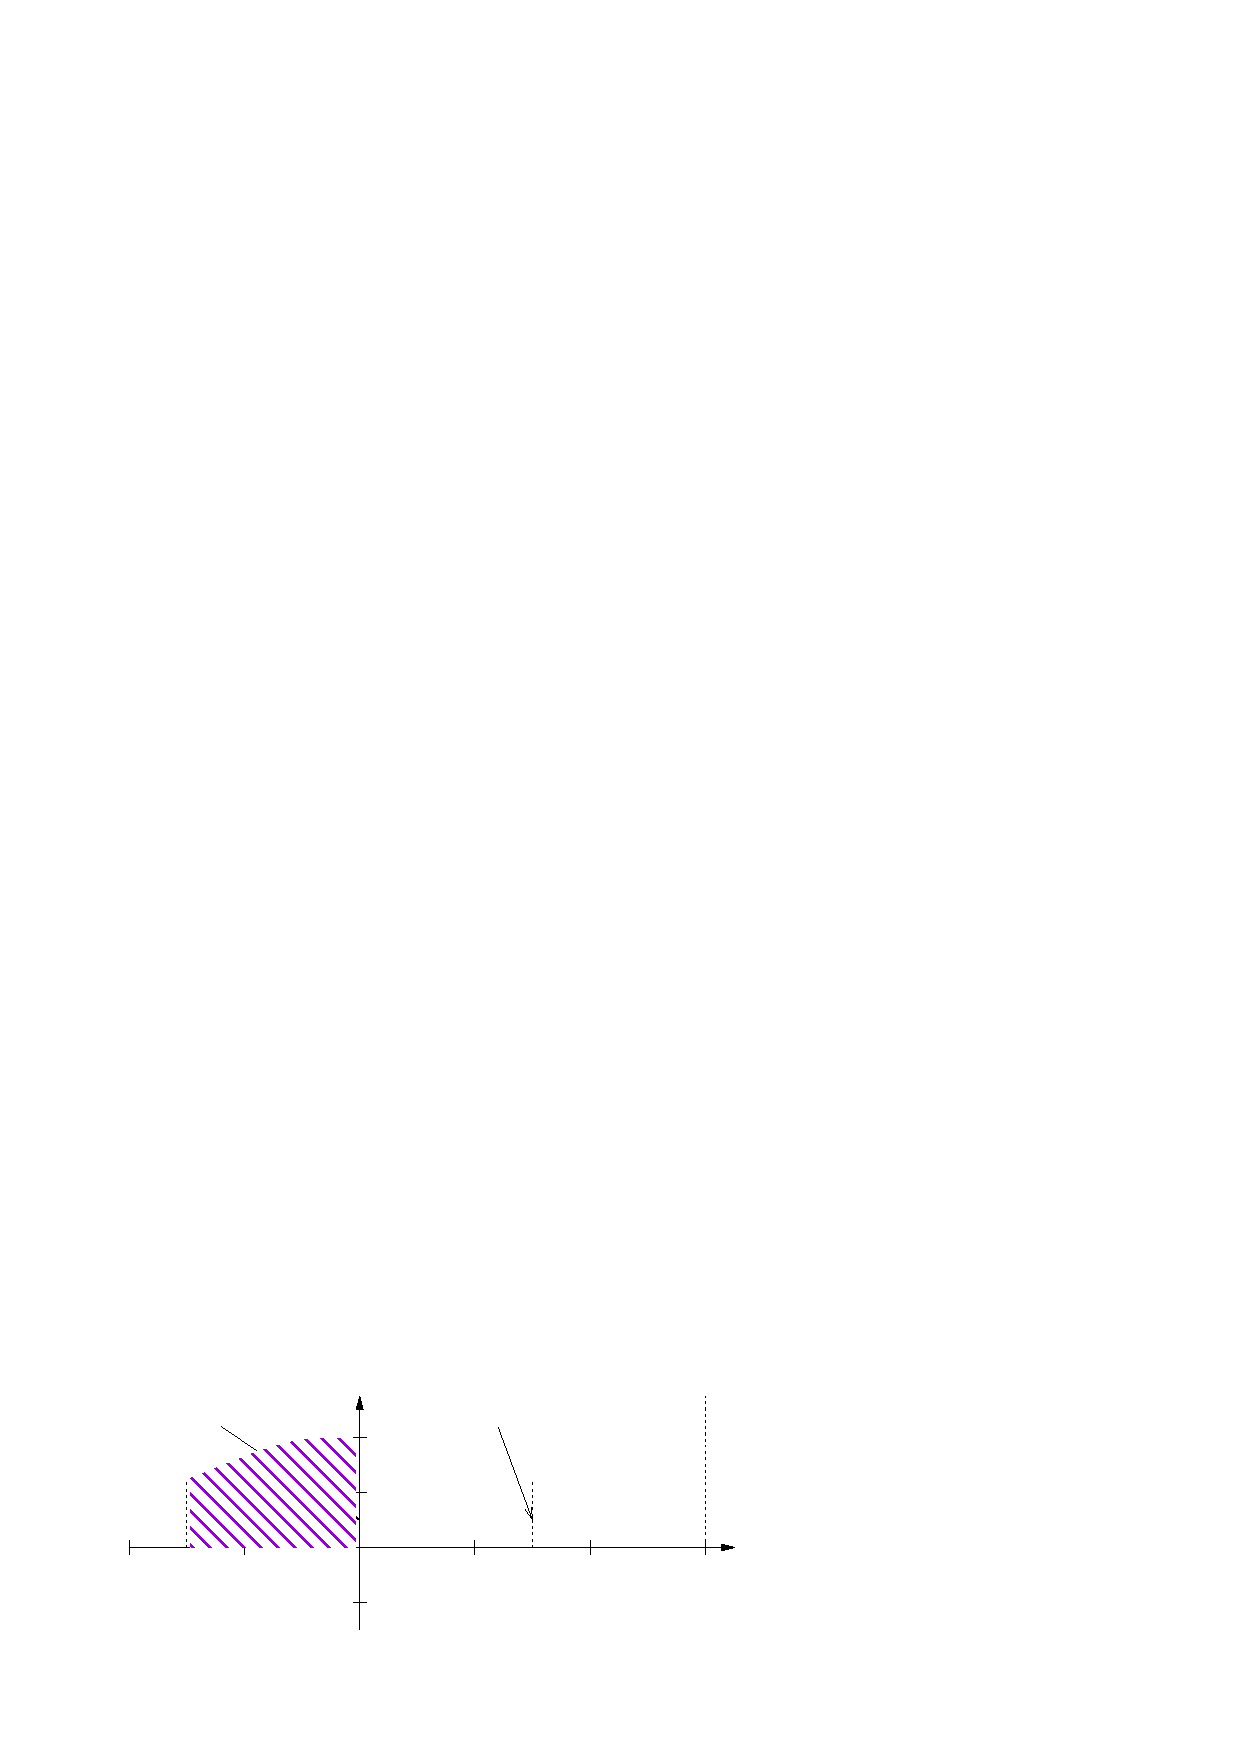
\includegraphics[width={316.80bp},height={129.50bp}]{figura_01_04}}%
    \gplfronttext
  \end{picture}%
\endgroup

    \caption{Demostración gráfica}\label{figura_04}
\end{figure}

\subsection*{Propiedad 4}
Si $b-a=T$:
\begin{equation}
    \int_{0}^{T}f(t)\,dt=\int_{a}^{b}f(t)\,dt
\label{propiedad4}
\end{equation}

\underline{Prueba}:

\begin{equation*}
\begin{split}
    \int_{a}^{b}f(t)\,dt
        &=\int_{a}^{a+T}f(t)\,dt\\
        &=\int_{a}^{T}f(t)\,dt+\int_{T}^{a+T}f(t)\,dt\\
        &=\int_{a}^{T}f(t)\,dt+\int_{T-T}^{a+T-T}f(t)\,dt\\
        &=\int_{a}^{T}f(t)\,dt+\int_{0}^{a}f(t)\,dt\\
        &=\int_{0}^{T}f(t)\,dt
\end{split}
\end{equation*}

Puede verse gráficamente en la \textbf{Figura~\ref{figura_05}}.
\begin{figure}[H]
    \centering
    % GNUPLOT: LaTeX picture with Postscript
\begingroup
  \makeatletter
  \providecommand\color[2][]{%
    \GenericError{(gnuplot) \space\space\space\@spaces}{%
      Package color not loaded in conjunction with
      terminal option `colourtext'%
    }{See the gnuplot documentation for explanation.%
    }{Either use 'blacktext' in gnuplot or load the package
      color.sty in LaTeX.}%
    \renewcommand\color[2][]{}%
  }%
  \providecommand\includegraphics[2][]{%
    \GenericError{(gnuplot) \space\space\space\@spaces}{%
      Package graphicx or graphics not loaded%
    }{See the gnuplot documentation for explanation.%
    }{The gnuplot epslatex terminal needs graphicx.sty or graphics.sty.}%
    \renewcommand\includegraphics[2][]{}%
  }%
  \providecommand\rotatebox[2]{#2}%
  \@ifundefined{ifGPcolor}{%
    \newif\ifGPcolor
    \GPcolorfalse
  }{}%
  \@ifundefined{ifGPblacktext}{%
    \newif\ifGPblacktext
    \GPblacktexttrue
  }{}%
  % define a \g@addto@macro without @ in the name:
  \let\gplgaddtomacro\g@addto@macro
  % define empty templates for all commands taking text:
  \gdef\gplbacktext{}%
  \gdef\gplfronttext{}%
  \makeatother
  \ifGPblacktext
    % no textcolor at all
    \def\colorrgb#1{}%
    \def\colorgray#1{}%
  \else
    % gray or color?
    \ifGPcolor
      \def\colorrgb#1{\color[rgb]{#1}}%
      \def\colorgray#1{\color[gray]{#1}}%
      \expandafter\def\csname LTw\endcsname{\color{white}}%
      \expandafter\def\csname LTb\endcsname{\color{black}}%
      \expandafter\def\csname LTa\endcsname{\color{black}}%
      \expandafter\def\csname LT0\endcsname{\color[rgb]{1,0,0}}%
      \expandafter\def\csname LT1\endcsname{\color[rgb]{0,1,0}}%
      \expandafter\def\csname LT2\endcsname{\color[rgb]{0,0,1}}%
      \expandafter\def\csname LT3\endcsname{\color[rgb]{1,0,1}}%
      \expandafter\def\csname LT4\endcsname{\color[rgb]{0,1,1}}%
      \expandafter\def\csname LT5\endcsname{\color[rgb]{1,1,0}}%
      \expandafter\def\csname LT6\endcsname{\color[rgb]{0,0,0}}%
      \expandafter\def\csname LT7\endcsname{\color[rgb]{1,0.3,0}}%
      \expandafter\def\csname LT8\endcsname{\color[rgb]{0.5,0.5,0.5}}%
    \else
      % gray
      \def\colorrgb#1{\color{black}}%
      \def\colorgray#1{\color[gray]{#1}}%
      \expandafter\def\csname LTw\endcsname{\color{white}}%
      \expandafter\def\csname LTb\endcsname{\color{black}}%
      \expandafter\def\csname LTa\endcsname{\color{black}}%
      \expandafter\def\csname LT0\endcsname{\color{black}}%
      \expandafter\def\csname LT1\endcsname{\color{black}}%
      \expandafter\def\csname LT2\endcsname{\color{black}}%
      \expandafter\def\csname LT3\endcsname{\color{black}}%
      \expandafter\def\csname LT4\endcsname{\color{black}}%
      \expandafter\def\csname LT5\endcsname{\color{black}}%
      \expandafter\def\csname LT6\endcsname{\color{black}}%
      \expandafter\def\csname LT7\endcsname{\color{black}}%
      \expandafter\def\csname LT8\endcsname{\color{black}}%
    \fi
  \fi
    \setlength{\unitlength}{0.0500bp}%
    \ifx\gptboxheight\undefined%
      \newlength{\gptboxheight}%
      \newlength{\gptboxwidth}%
      \newsavebox{\gptboxtext}%
    \fi%
    \setlength{\fboxrule}{0.5pt}%
    \setlength{\fboxsep}{1pt}%
    \definecolor{tbcol}{rgb}{1,1,1}%
\begin{picture}(6336.00,2590.00)%
    \gplgaddtomacro\gplbacktext{%
      \csname LTb\endcsname%%
      \put(1233,416){\makebox(0,0)[r]{\strut{}}}%
      \put(1233,863){\makebox(0,0)[r]{\strut{}}}%
      \put(1233,1311){\makebox(0,0)[r]{\strut{}}}%
      \put(1233,1758){\makebox(0,0)[r]{\strut{}}}%
      \put(1233,2205){\makebox(0,0)[r]{\strut{}}}%
      \put(603,640){\makebox(0,0){\strut{}}}%
      \put(1329,640){\makebox(0,0){\strut{}}}%
      \put(2055,640){\makebox(0,0){\strut{}}}%
      \put(2781,640){\makebox(0,0){\strut{}}}%
      \put(3506,640){\makebox(0,0){\strut{}}}%
      \put(4232,640){\makebox(0,0){\strut{}}}%
      \put(4958,640){\makebox(0,0){\strut{}}}%
      \put(5684,640){\makebox(0,0){\strut{}}}%
      \csname LTb\endcsname%%
      \put(6228,863){\makebox(0,0)[l]{\strut{}$t$}}%
      \put(1502,2429){\makebox(0,0)[l]{\strut{}$f(t)$}}%
      \put(2756,662){\makebox(0,0)[l]{\strut{}$a$}}%
      \put(3435,662){\makebox(0,0)[l]{\strut{}$T$}}%
      \put(4887,662){\makebox(0,0)[l]{\strut{}$b$}}%
      \put(1766,2026){\makebox(0,0)[l]{\strut{}$\int_{0}^{T} f(t) dt$}}%
      \put(3943,2295){\makebox(0,0)[l]{\strut{}$\int_{a}^{b} f(t) dt$}}%
      \put(3770,259){\makebox(0,0)[l]{\strut{}$T$}}%
    }%
    \gplgaddtomacro\gplfronttext{%
    }%
    \gplgaddtomacro\gplbacktext{%
      \csname LTb\endcsname%%
      \put(1233,416){\makebox(0,0)[r]{\strut{}}}%
      \put(1233,863){\makebox(0,0)[r]{\strut{}}}%
      \put(1233,1311){\makebox(0,0)[r]{\strut{}}}%
      \put(1233,1758){\makebox(0,0)[r]{\strut{}}}%
      \put(1233,2205){\makebox(0,0)[r]{\strut{}}}%
      \put(603,640){\makebox(0,0){\strut{}}}%
      \put(1329,640){\makebox(0,0){\strut{}}}%
      \put(2055,640){\makebox(0,0){\strut{}}}%
      \put(2781,640){\makebox(0,0){\strut{}}}%
      \put(3506,640){\makebox(0,0){\strut{}}}%
      \put(4232,640){\makebox(0,0){\strut{}}}%
      \put(4958,640){\makebox(0,0){\strut{}}}%
      \put(5684,640){\makebox(0,0){\strut{}}}%
      \csname LTb\endcsname%%
      \put(6228,863){\makebox(0,0)[l]{\strut{}$t$}}%
      \put(1502,2429){\makebox(0,0)[l]{\strut{}$f(t)$}}%
      \put(2756,662){\makebox(0,0)[l]{\strut{}$a$}}%
      \put(3435,662){\makebox(0,0)[l]{\strut{}$T$}}%
      \put(4887,662){\makebox(0,0)[l]{\strut{}$b$}}%
      \put(1766,2026){\makebox(0,0)[l]{\strut{}$\int_{0}^{T} f(t) dt$}}%
      \put(3943,2295){\makebox(0,0)[l]{\strut{}$\int_{a}^{b} f(t) dt$}}%
      \put(3770,259){\makebox(0,0)[l]{\strut{}$T$}}%
    }%
    \gplgaddtomacro\gplfronttext{%
    }%
    \gplgaddtomacro\gplbacktext{%
      \csname LTb\endcsname%%
      \put(1233,416){\makebox(0,0)[r]{\strut{}}}%
      \put(1233,863){\makebox(0,0)[r]{\strut{}}}%
      \put(1233,1311){\makebox(0,0)[r]{\strut{}}}%
      \put(1233,1758){\makebox(0,0)[r]{\strut{}}}%
      \put(1233,2205){\makebox(0,0)[r]{\strut{}}}%
      \put(603,640){\makebox(0,0){\strut{}}}%
      \put(1329,640){\makebox(0,0){\strut{}}}%
      \put(2055,640){\makebox(0,0){\strut{}}}%
      \put(2781,640){\makebox(0,0){\strut{}}}%
      \put(3506,640){\makebox(0,0){\strut{}}}%
      \put(4232,640){\makebox(0,0){\strut{}}}%
      \put(4958,640){\makebox(0,0){\strut{}}}%
      \put(5684,640){\makebox(0,0){\strut{}}}%
      \csname LTb\endcsname%%
      \put(6228,863){\makebox(0,0)[l]{\strut{}$t$}}%
      \put(1502,2429){\makebox(0,0)[l]{\strut{}$f(t)$}}%
      \put(2756,662){\makebox(0,0)[l]{\strut{}$a$}}%
      \put(3435,662){\makebox(0,0)[l]{\strut{}$T$}}%
      \put(4887,662){\makebox(0,0)[l]{\strut{}$b$}}%
      \put(1766,2026){\makebox(0,0)[l]{\strut{}$\int_{0}^{T} f(t) dt$}}%
      \put(3943,2295){\makebox(0,0)[l]{\strut{}$\int_{a}^{b} f(t) dt$}}%
      \put(3770,259){\makebox(0,0)[l]{\strut{}$T$}}%
    }%
    \gplgaddtomacro\gplfronttext{%
    }%
    \gplgaddtomacro\gplbacktext{%
      \csname LTb\endcsname%%
      \put(1233,416){\makebox(0,0)[r]{\strut{}}}%
      \put(1233,863){\makebox(0,0)[r]{\strut{}}}%
      \put(1233,1311){\makebox(0,0)[r]{\strut{}}}%
      \put(1233,1758){\makebox(0,0)[r]{\strut{}}}%
      \put(1233,2205){\makebox(0,0)[r]{\strut{}}}%
      \put(603,640){\makebox(0,0){\strut{}}}%
      \put(1329,640){\makebox(0,0){\strut{}}}%
      \put(2055,640){\makebox(0,0){\strut{}}}%
      \put(2781,640){\makebox(0,0){\strut{}}}%
      \put(3506,640){\makebox(0,0){\strut{}}}%
      \put(4232,640){\makebox(0,0){\strut{}}}%
      \put(4958,640){\makebox(0,0){\strut{}}}%
      \put(5684,640){\makebox(0,0){\strut{}}}%
      \csname LTb\endcsname%%
      \put(6228,863){\makebox(0,0)[l]{\strut{}$t$}}%
      \put(1502,2429){\makebox(0,0)[l]{\strut{}$f(t)$}}%
      \put(2756,662){\makebox(0,0)[l]{\strut{}$a$}}%
      \put(3435,662){\makebox(0,0)[l]{\strut{}$T$}}%
      \put(4887,662){\makebox(0,0)[l]{\strut{}$b$}}%
      \put(1766,2026){\makebox(0,0)[l]{\strut{}$\int_{0}^{T} f(t) dt$}}%
      \put(3943,2295){\makebox(0,0)[l]{\strut{}$\int_{a}^{b} f(t) dt$}}%
      \put(3770,259){\makebox(0,0)[l]{\strut{}$T$}}%
    }%
    \gplgaddtomacro\gplfronttext{%
    }%
    \gplgaddtomacro\gplbacktext{%
      \csname LTb\endcsname%%
      \put(1233,416){\makebox(0,0)[r]{\strut{}}}%
      \put(1233,863){\makebox(0,0)[r]{\strut{}}}%
      \put(1233,1311){\makebox(0,0)[r]{\strut{}}}%
      \put(1233,1758){\makebox(0,0)[r]{\strut{}}}%
      \put(1233,2205){\makebox(0,0)[r]{\strut{}}}%
      \put(603,640){\makebox(0,0){\strut{}}}%
      \put(1329,640){\makebox(0,0){\strut{}}}%
      \put(2055,640){\makebox(0,0){\strut{}}}%
      \put(2781,640){\makebox(0,0){\strut{}}}%
      \put(3506,640){\makebox(0,0){\strut{}}}%
      \put(4232,640){\makebox(0,0){\strut{}}}%
      \put(4958,640){\makebox(0,0){\strut{}}}%
      \put(5684,640){\makebox(0,0){\strut{}}}%
      \csname LTb\endcsname%%
      \put(6228,863){\makebox(0,0)[l]{\strut{}$t$}}%
      \put(1502,2429){\makebox(0,0)[l]{\strut{}$f(t)$}}%
      \put(2756,662){\makebox(0,0)[l]{\strut{}$a$}}%
      \put(3435,662){\makebox(0,0)[l]{\strut{}$T$}}%
      \put(4887,662){\makebox(0,0)[l]{\strut{}$b$}}%
      \put(1766,2026){\makebox(0,0)[l]{\strut{}$\int_{0}^{T} f(t) dt$}}%
      \put(3943,2295){\makebox(0,0)[l]{\strut{}$\int_{a}^{b} f(t) dt$}}%
      \put(3770,259){\makebox(0,0)[l]{\strut{}$T$}}%
    }%
    \gplgaddtomacro\gplfronttext{%
    }%
    \gplgaddtomacro\gplbacktext{%
      \csname LTb\endcsname%%
      \put(1233,416){\makebox(0,0)[r]{\strut{}}}%
      \put(1233,863){\makebox(0,0)[r]{\strut{}}}%
      \put(1233,1311){\makebox(0,0)[r]{\strut{}}}%
      \put(1233,1758){\makebox(0,0)[r]{\strut{}}}%
      \put(1233,2205){\makebox(0,0)[r]{\strut{}}}%
      \put(603,640){\makebox(0,0){\strut{}}}%
      \put(1329,640){\makebox(0,0){\strut{}}}%
      \put(2055,640){\makebox(0,0){\strut{}}}%
      \put(2781,640){\makebox(0,0){\strut{}}}%
      \put(3506,640){\makebox(0,0){\strut{}}}%
      \put(4232,640){\makebox(0,0){\strut{}}}%
      \put(4958,640){\makebox(0,0){\strut{}}}%
      \put(5684,640){\makebox(0,0){\strut{}}}%
      \csname LTb\endcsname%%
      \put(6228,863){\makebox(0,0)[l]{\strut{}$t$}}%
      \put(1502,2429){\makebox(0,0)[l]{\strut{}$f(t)$}}%
      \put(2756,662){\makebox(0,0)[l]{\strut{}$a$}}%
      \put(3435,662){\makebox(0,0)[l]{\strut{}$T$}}%
      \put(4887,662){\makebox(0,0)[l]{\strut{}$b$}}%
      \put(1766,2026){\makebox(0,0)[l]{\strut{}$\int_{0}^{T} f(t) dt$}}%
      \put(3943,2295){\makebox(0,0)[l]{\strut{}$\int_{a}^{b} f(t) dt$}}%
      \put(3770,259){\makebox(0,0)[l]{\strut{}$T$}}%
    }%
    \gplgaddtomacro\gplfronttext{%
    }%
    \gplgaddtomacro\gplbacktext{%
      \csname LTb\endcsname%%
      \put(1233,416){\makebox(0,0)[r]{\strut{}}}%
      \put(1233,863){\makebox(0,0)[r]{\strut{}}}%
      \put(1233,1311){\makebox(0,0)[r]{\strut{}}}%
      \put(1233,1758){\makebox(0,0)[r]{\strut{}}}%
      \put(1233,2205){\makebox(0,0)[r]{\strut{}}}%
      \put(603,640){\makebox(0,0){\strut{}}}%
      \put(1329,640){\makebox(0,0){\strut{}}}%
      \put(2055,640){\makebox(0,0){\strut{}}}%
      \put(2781,640){\makebox(0,0){\strut{}}}%
      \put(3506,640){\makebox(0,0){\strut{}}}%
      \put(4232,640){\makebox(0,0){\strut{}}}%
      \put(4958,640){\makebox(0,0){\strut{}}}%
      \put(5684,640){\makebox(0,0){\strut{}}}%
      \csname LTb\endcsname%%
      \put(6228,863){\makebox(0,0)[l]{\strut{}$t$}}%
      \put(1502,2429){\makebox(0,0)[l]{\strut{}$f(t)$}}%
      \put(2756,662){\makebox(0,0)[l]{\strut{}$a$}}%
      \put(3435,662){\makebox(0,0)[l]{\strut{}$T$}}%
      \put(4887,662){\makebox(0,0)[l]{\strut{}$b$}}%
      \put(1766,2026){\makebox(0,0)[l]{\strut{}$\int_{0}^{T} f(t) dt$}}%
      \put(3943,2295){\makebox(0,0)[l]{\strut{}$\int_{a}^{b} f(t) dt$}}%
      \put(3770,259){\makebox(0,0)[l]{\strut{}$T$}}%
    }%
    \gplgaddtomacro\gplfronttext{%
    }%
    \gplbacktext
    \put(0,0){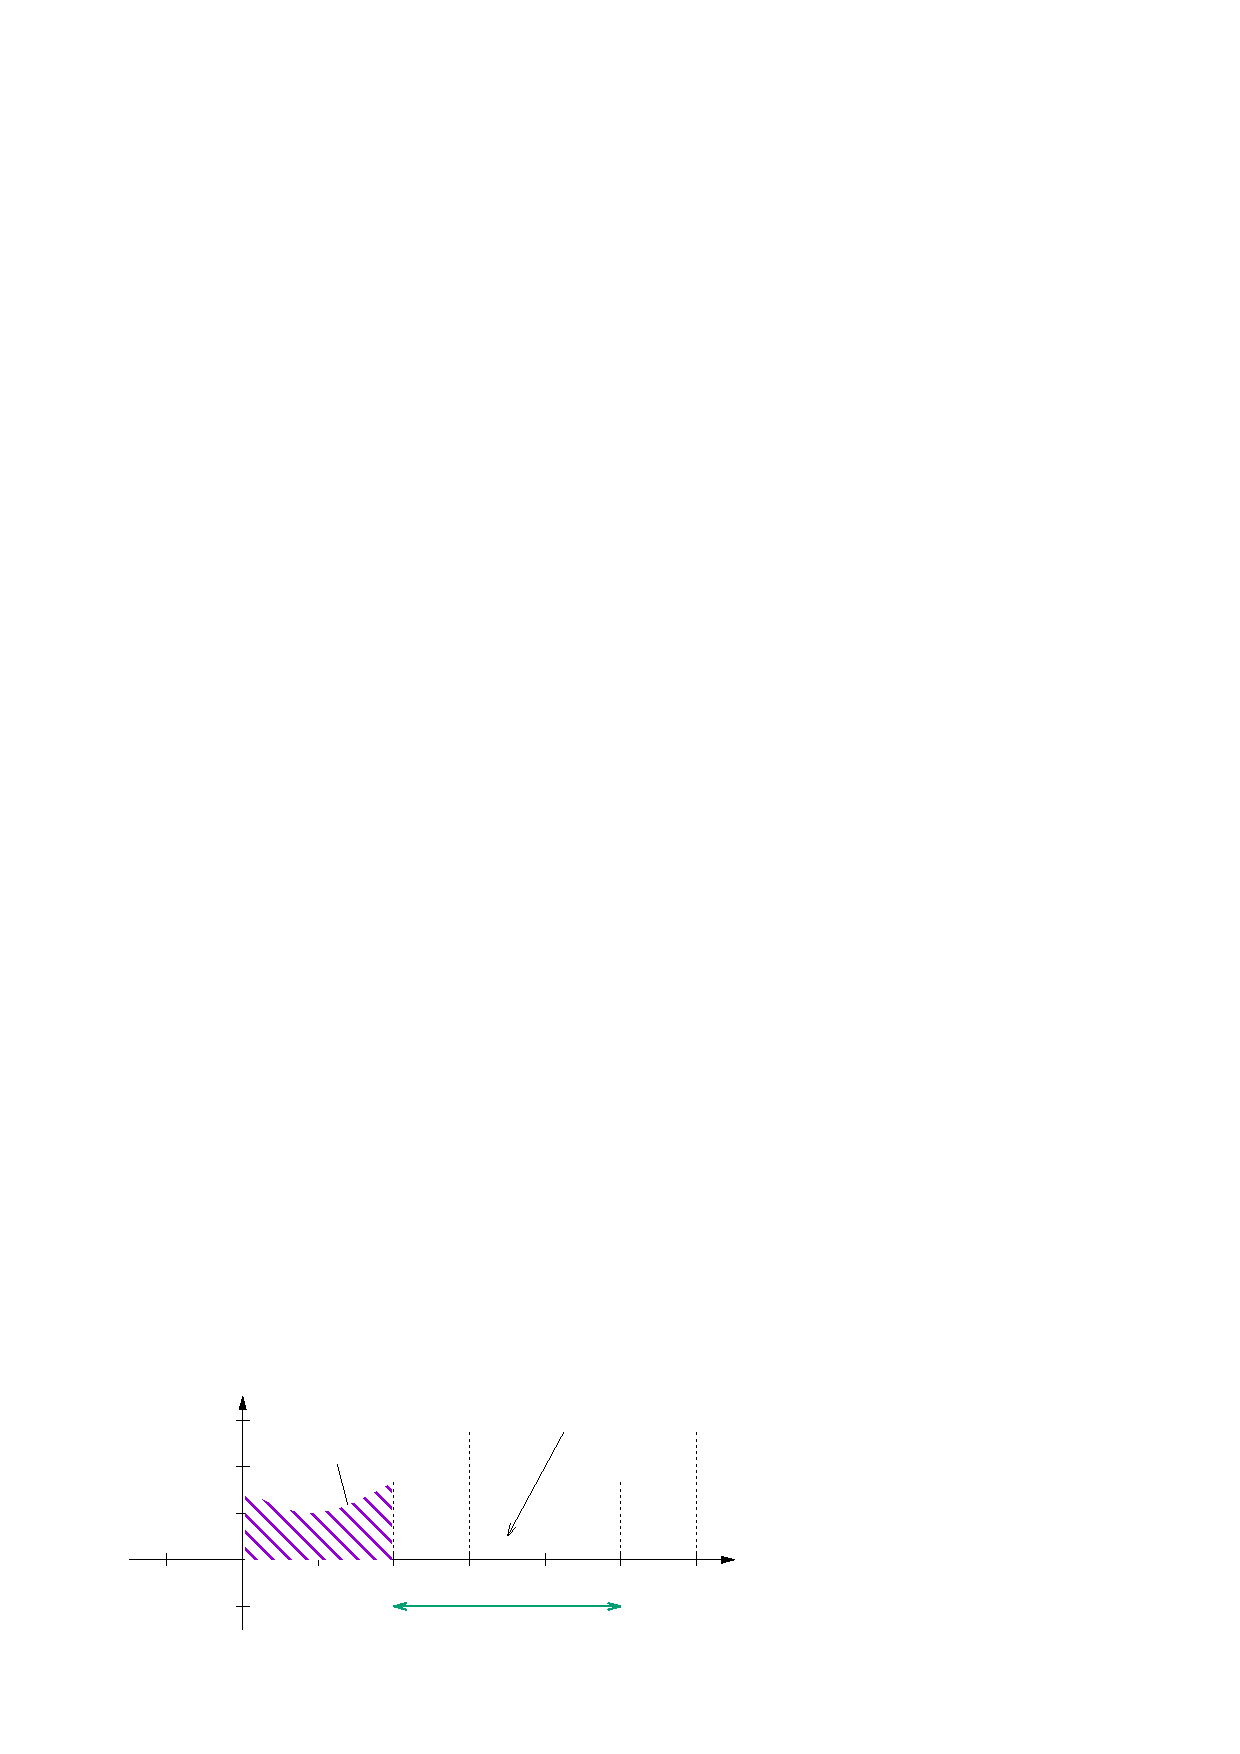
\includegraphics[width={316.80bp},height={129.50bp}]{figura_01_05}}%
    \gplfronttext
  \end{picture}%
\endgroup

    \caption{Demostración gráfica}\label{figura_05}
\end{figure}

\subsection{Funciones seno y coseno}
\begin{equation*}
    f(t)=A\,\sen(\omega_0\,t)
\end{equation*}
\begin{equation*}
    f(t)=A\,\cos(\omega_0\,t)
\end{equation*}

Donde:\\
\indent\indent$A$: Amplitud.\\
\indent\indent$\omega_0$: Frecuencia angular.\\
\indent\indent$T=2\pi/\omega_0$: Periodo.\\

\textbf{Ejemplo}: Hallar el periodo de la siguiente función:
\begin{equation*}
    f(t)=\sen(4t)+\sen(3t/2)+\sen(10t)
\end{equation*}

El periodo buscado debe contener un numero entero de veces a los 3 periodos
hallados:
\begin{equation*}
    T=\begin{cases}
        a\,T_1;&\,a\in\mathbb{N}\\
        b\,T_2;&\,b\in\mathbb{N}\\
        c\,T_3;&\,c\in\mathbb{N}\\
    \end{cases}
\end{equation*}
\begin{equation*}
    a\,T_1=b\,T_2=c\,T_3
\end{equation*}
\begin{equation*}
    a\,\frac{2\pi}{4}=b\,\frac{2\pi}{3/2}=c\,\frac{2\pi}{10}
\end{equation*}
\begin{equation*}
    a\,\frac{\pi}{2}=b\,\frac{4\pi}{3}=c\,\frac{\pi}{5};x30
\end{equation*}
\begin{equation*}
    15a=40b=6c
\end{equation*}
\begin{equation*}
    M.C.M.(15,40,6)=120
\end{equation*}
\begin{equation*}
\left.\begin{aligned}
    120=15a\rightarrow\,a=8\\
    120=40b\rightarrow\,b=3\\
    120=6c\rightarrow\,c=20\\
\end{aligned}\right\}=T=8\left(\frac{\pi}{2}\right)=4\pi
\end{equation*}

Puede verse gráficamente en la \textbf{Figura~\ref{figura_06}}.
\begin{figure}[H]
    \centering
    % GNUPLOT: LaTeX picture with Postscript
\begingroup
  \makeatletter
  \providecommand\color[2][]{%
    \GenericError{(gnuplot) \space\space\space\@spaces}{%
      Package color not loaded in conjunction with
      terminal option `colourtext'%
    }{See the gnuplot documentation for explanation.%
    }{Either use 'blacktext' in gnuplot or load the package
      color.sty in LaTeX.}%
    \renewcommand\color[2][]{}%
  }%
  \providecommand\includegraphics[2][]{%
    \GenericError{(gnuplot) \space\space\space\@spaces}{%
      Package graphicx or graphics not loaded%
    }{See the gnuplot documentation for explanation.%
    }{The gnuplot epslatex terminal needs graphicx.sty or graphics.sty.}%
    \renewcommand\includegraphics[2][]{}%
  }%
  \providecommand\rotatebox[2]{#2}%
  \@ifundefined{ifGPcolor}{%
    \newif\ifGPcolor
    \GPcolorfalse
  }{}%
  \@ifundefined{ifGPblacktext}{%
    \newif\ifGPblacktext
    \GPblacktexttrue
  }{}%
  % define a \g@addto@macro without @ in the name:
  \let\gplgaddtomacro\g@addto@macro
  % define empty templates for all commands taking text:
  \gdef\gplbacktext{}%
  \gdef\gplfronttext{}%
  \makeatother
  \ifGPblacktext
    % no textcolor at all
    \def\colorrgb#1{}%
    \def\colorgray#1{}%
  \else
    % gray or color?
    \ifGPcolor
      \def\colorrgb#1{\color[rgb]{#1}}%
      \def\colorgray#1{\color[gray]{#1}}%
      \expandafter\def\csname LTw\endcsname{\color{white}}%
      \expandafter\def\csname LTb\endcsname{\color{black}}%
      \expandafter\def\csname LTa\endcsname{\color{black}}%
      \expandafter\def\csname LT0\endcsname{\color[rgb]{1,0,0}}%
      \expandafter\def\csname LT1\endcsname{\color[rgb]{0,1,0}}%
      \expandafter\def\csname LT2\endcsname{\color[rgb]{0,0,1}}%
      \expandafter\def\csname LT3\endcsname{\color[rgb]{1,0,1}}%
      \expandafter\def\csname LT4\endcsname{\color[rgb]{0,1,1}}%
      \expandafter\def\csname LT5\endcsname{\color[rgb]{1,1,0}}%
      \expandafter\def\csname LT6\endcsname{\color[rgb]{0,0,0}}%
      \expandafter\def\csname LT7\endcsname{\color[rgb]{1,0.3,0}}%
      \expandafter\def\csname LT8\endcsname{\color[rgb]{0.5,0.5,0.5}}%
    \else
      % gray
      \def\colorrgb#1{\color{black}}%
      \def\colorgray#1{\color[gray]{#1}}%
      \expandafter\def\csname LTw\endcsname{\color{white}}%
      \expandafter\def\csname LTb\endcsname{\color{black}}%
      \expandafter\def\csname LTa\endcsname{\color{black}}%
      \expandafter\def\csname LT0\endcsname{\color{black}}%
      \expandafter\def\csname LT1\endcsname{\color{black}}%
      \expandafter\def\csname LT2\endcsname{\color{black}}%
      \expandafter\def\csname LT3\endcsname{\color{black}}%
      \expandafter\def\csname LT4\endcsname{\color{black}}%
      \expandafter\def\csname LT5\endcsname{\color{black}}%
      \expandafter\def\csname LT6\endcsname{\color{black}}%
      \expandafter\def\csname LT7\endcsname{\color{black}}%
      \expandafter\def\csname LT8\endcsname{\color{black}}%
    \fi
  \fi
    \setlength{\unitlength}{0.0500bp}%
    \ifx\gptboxheight\undefined%
      \newlength{\gptboxheight}%
      \newlength{\gptboxwidth}%
      \newsavebox{\gptboxtext}%
    \fi%
    \setlength{\fboxrule}{0.5pt}%
    \setlength{\fboxsep}{1pt}%
    \definecolor{tbcol}{rgb}{1,1,1}%
\begin{picture}(6336.00,1872.00)%
    \gplgaddtomacro\gplbacktext{%
      \csname LTb\endcsname%%
      \put(144,276){\makebox(0,0)[r]{\strut{}}}%
      \put(144,445){\makebox(0,0)[r]{\strut{}}}%
      \put(144,614){\makebox(0,0)[r]{\strut{}}}%
      \put(144,783){\makebox(0,0)[r]{\strut{}}}%
      \put(144,952){\makebox(0,0)[r]{\strut{}}}%
      \put(144,1120){\makebox(0,0)[r]{\strut{}}}%
      \put(144,1289){\makebox(0,0)[r]{\strut{}}}%
      \put(144,1458){\makebox(0,0)[r]{\strut{}}}%
      \put(144,1627){\makebox(0,0)[r]{\strut{}}}%
      \put(240,560){\makebox(0,0){\strut{}}}%
      \put(1606,560){\makebox(0,0){\strut{}}}%
      \put(2973,560){\makebox(0,0){\strut{}}}%
      \put(4339,560){\makebox(0,0){\strut{}}}%
      \put(5705,560){\makebox(0,0){\strut{}}}%
      \csname LTb\endcsname%%
      \put(6184,783){\makebox(0,0)[l]{\strut{}$t$}}%
      \put(392,1711){\makebox(0,0)[l]{\strut{}$f(t)$}}%
      \put(1541,656){\makebox(0,0)[l]{\strut{}$ \pi$}}%
      \put(2907,656){\makebox(0,0)[l]{\strut{}$2\pi$}}%
      \put(4274,656){\makebox(0,0)[l]{\strut{}$3\pi$}}%
      \put(5640,656){\makebox(0,0)[l]{\strut{}$4\pi$}}%
      \put(1606,1593){\makebox(0,0)[l]{\strut{}$f(t)=\sen(4t)+\sen(\frac{3}{2}t)+\sen(10t)\,dt$}}%
    }%
    \gplgaddtomacro\gplfronttext{%
    }%
    \gplbacktext
    \put(0,0){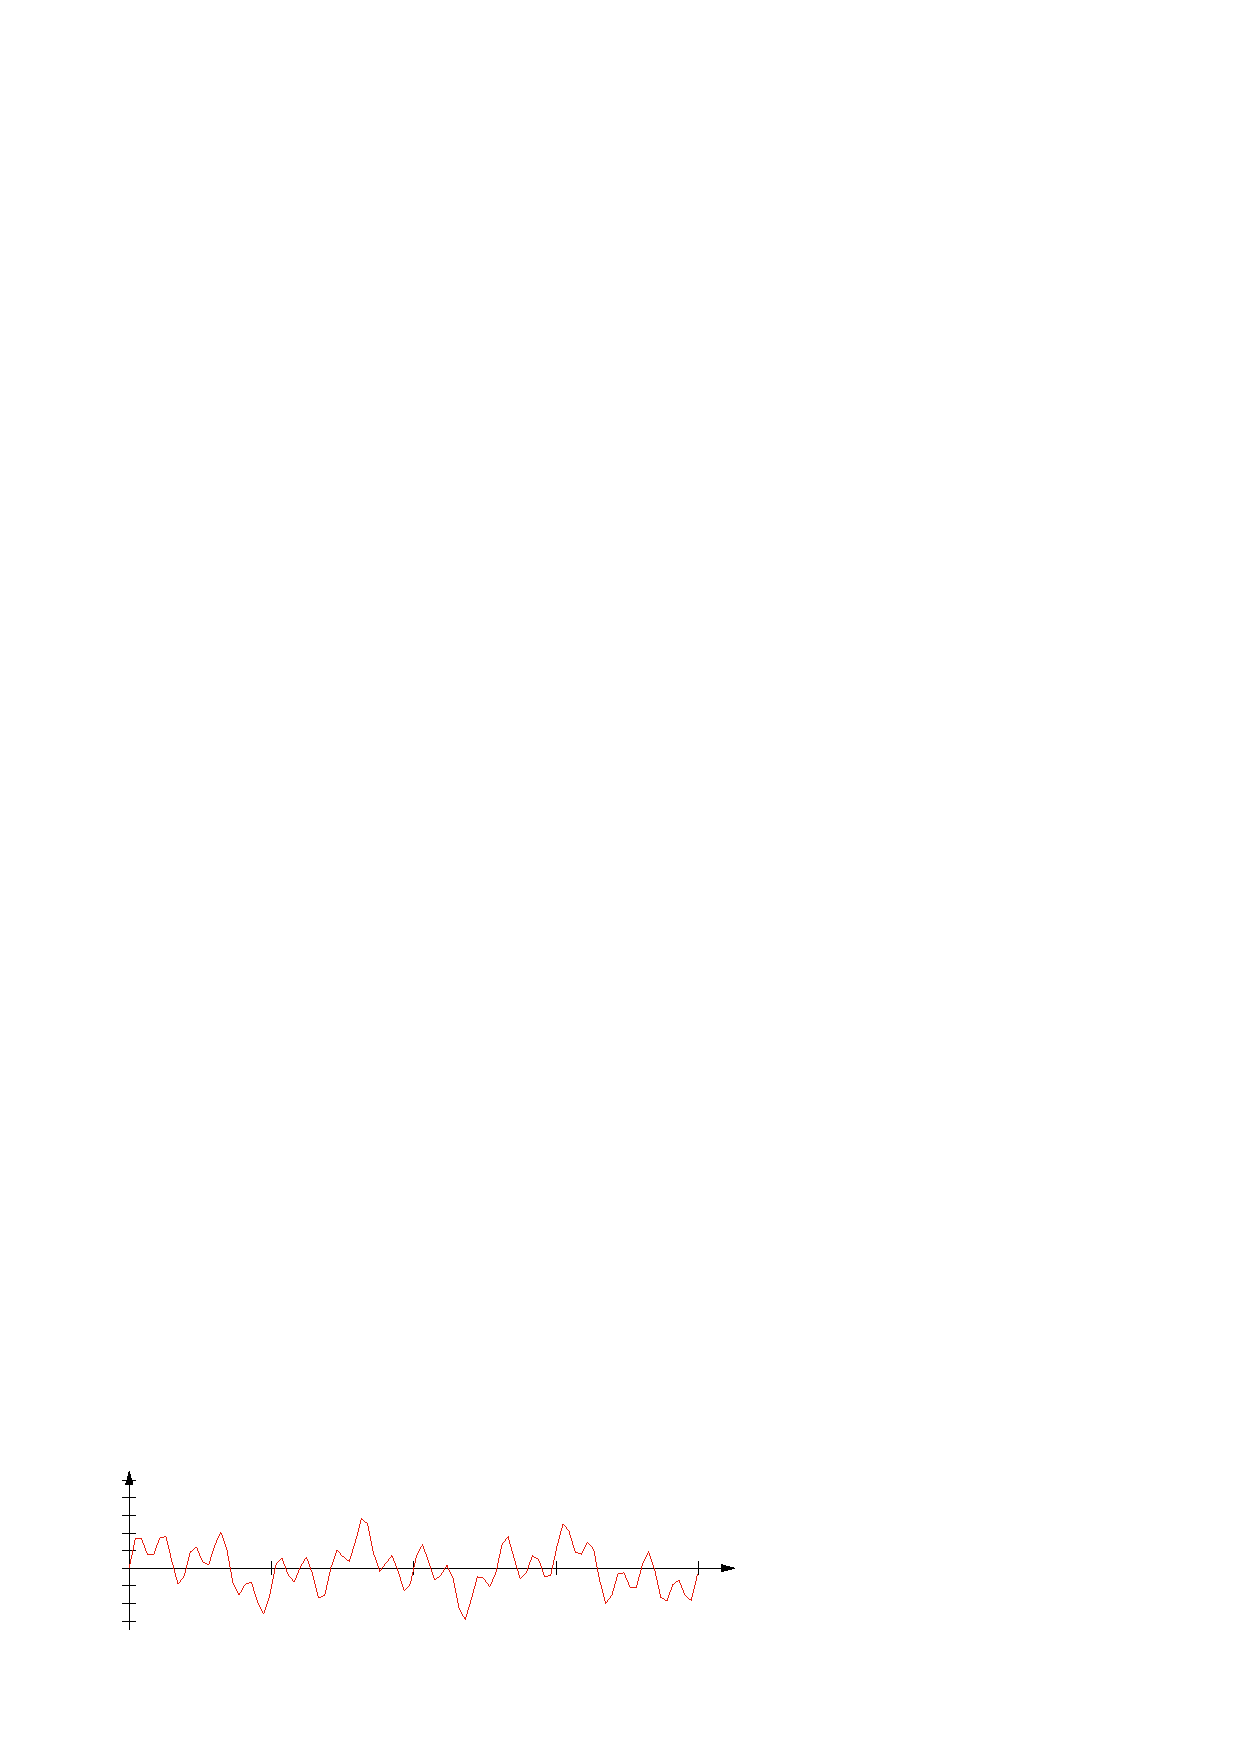
\includegraphics[width={316.80bp},height={93.60bp}]{figura_01_06}}%
    \gplfronttext
  \end{picture}%
\endgroup

    \caption{Periodo de la función}\label{figura_06}
\end{figure}

\subsection{Propiedades ortogonales del seno y el coseno}
\subsection*{Propiedad 1}
\begin{equation}
    \int_{0}^{T}\sen(n\omega_0\,t)\,dt=0\quad\,n\in\mathbb{Z}
\end{equation}

\underline{Prueba}:

\begin{equation*}
\begin{split}
    \int_{0}^{T}\sen(n\omega_0\,t)\,dt
        &=-\frac{\cos(n\omega_0\,t)}{n\omega_0}\Biggr|_{0}^{T}\\
        &=-\frac{\cos(n\omega_0\,T)}{n\omega_0}+\frac{\cos(0)}{n\omega_0}\\
        &=-\frac{\cos(n\,2\pi)}{n\omega_0}+\frac{\cos(0)}{n\omega_0}\\
        &=-\frac{1}{n\omega_0}+\frac{1}{n\omega_0}\\
        &=0\\
\end{split}
\end{equation*}
\begin{equation}
    \int_{0}^{T}\cos(n\omega_0\,t)\,dt=0\quad\,n\in\mathbb{Z}
\end{equation}

\underline{Prueba}:

\begin{equation*}
\begin{split}
    \int_{0}^{T}\cos(n\omega_0\,t)\,dt
        &=\frac{\sen(n\omega_0\,t)}{n\omega_0}\Biggr|_{0}^{T}\\
        &=\frac{\sen(n\omega_0\,T)}{n\omega_0}-\frac{\sen(0)}{n\omega_0}\\
        &=\frac{\sen(n\,2\pi)}{n\omega_0}-\frac{\sen(0)}{n\omega_0}\\
        &=\frac{0}{n\omega_0}-\frac{0}{n\omega_0}\\
        &=0\\
\end{split}
\end{equation*}

\subsection*{Propiedad 2}
\begin{equation}
    \int_{0}^{T}\sen(m\omega_0\,t)\sen(n\omega_0\,t)\,dt=0
    \quad\,m,n\,\in\mathbb{Z}\quad\,m\neq\,n
\end{equation}

\underline{Prueba}:

\begin{equation*}
\begin{split}
    \int_{0}^{T}\sen(m\omega_0\,t)\sen(n\omega_0\,t)\,dt
        &=\int_{0}^{T}\frac{1}{2}(\cos((m-n)\omega_0\,t)-
          \cos((m+n)\omega_0\,t))dt\\
        &=\frac{1}{2}\left(\int_{0}^{T}\cos((m-n)\omega_0\,t)dt-
          \int_{0}^{T}\cos((m+n)\omega_0\,t)dt\right)\\
        &=\frac{1}{2}(0-0)\\
        &=0\\
\end{split}
\end{equation*}
\begin{equation}
    \int_{0}^{T}\cos(m\omega_0\,t)\cos(n\omega_0\,t)\,dt=0
    \quad\,m,n\,\in\mathbb{Z}\quad\,m\neq\,n
\end{equation}

\underline{Prueba}:

\begin{equation*}
\begin{split}
    \int_{0}^{T}\cos(m\omega_0\,t)\cos(n\omega_0\,t)\,dt
        &=\int_{0}^{T}\frac{1}{2}(\cos((m-n)\omega_0\,t)+
          \cos((m+n)\omega_0\,t))dt\\
        &=\frac{1}{2}\left(\int_{0}^{T}\cos((m-n)\omega_0\,t)dt+
          \int_{0}^{T}\cos((m+n)\omega_0\,t)dt\right)\\
        &=\frac{1}{2}(0+0)\\
        &=0\\
\end{split}
\end{equation*}
\begin{equation}
    \int_{0}^{T}\sen(m\omega_0\,t)\cos(n\omega_0\,t)\,dt
    =0\quad\,m,n\,\in\mathbb{Z}
\end{equation}

\underline{Prueba}:

\begin{equation*}
\begin{split}
    \int_{0}^{T}\sen(m\omega_0\,t)\cos(n\omega_0\,t)\,dt
        &=\int_{0}^{T}\frac{1}{2}(\sen((m-n)\omega_0\,t)+
          \sen((m+n)\omega_0\,t))dt\\
        &=\frac{1}{2}\left(\int_{0}^{T}\sen((m-n)\omega_0\,t)dt+
          \int_{0}^{T}\cos((m+n)\omega_0\,t)dt\right)\\
        &=\frac{1}{2}(0+0)\\
        &=0\\
\end{split}
\end{equation*}

\subsection*{Propiedad 3}
\begin{equation}
    \int_{0}^{T}\sen^2(n\omega_0\,t)\,dt=\frac{T}{2}\quad\,n\,\in\mathbb{Z}
\end{equation}

\underline{Prueba}:

\begin{equation*}
\begin{split}
    \int_{0}^{T}\sen^2(n\omega_0\,t)\,dt
        &=\int_{0}^{T}\sen(n\omega_0\,t)\sen(n\omega_0\,t)dt\\
        &=\frac{1}{2}\left(\int_{0}^{T}\cos((n-n)\omega_0\,t)dt-
          \int_{0}^{T}\cos((n+n)\omega_0\,t)dt\right)\\
        &=\frac{1}{2}\left(\int_{0}^{T}\cos(0)dt-
          \int_{0}^{T}\cos((2n)\omega_0\,t)dt\right)\\
        &=\frac{1}{2}\left(\int_{0}^{T}dt-
          \int_{0}^{T}\cos(2n\omega_0\,t)dt\right)\\
        &=\frac{1}{2}(t\Biggr|_0^T-0)\\
        &=\frac{T}{2}\\
\end{split}
\end{equation*}
\begin{equation}
    \int_{0}^{T}\cos^2(n\omega_0\,t)\,dt=\frac{T}{2}\quad\,n\,\in\mathbb{Z}
\end{equation}

\underline{Prueba}:

\begin{equation*}
\begin{split}
    \int_{0}^{T}\cos^2(n\omega_0\,t)\,dt
        &=\int_{0}^{T}\cos(n\omega_0\,t)\cos(n\omega_0\,t)dt\\
        &=\frac{1}{2}\left(\int_{0}^{T}\cos((n-n)\omega_0\,t)dt+
          \int_{0}^{T}\cos((n+n)\omega_0\,t)dt\right)\\
        &=\frac{1}{2}\left(\int_{0}^{T}\cos(0)dt+
          \int_{0}^{T}\cos((2n)\omega_0\,t)dt\right)\\
        &=\frac{1}{2}\left(\int_{0}^{T}dt+
          \int_{0}^{T}\cos(2n\omega_0\,t)dt\right)\\
        &=\frac{1}{2}(t\Biggr|_0^T+0)\\
        &=\frac{T}{2}\\
\end{split}
\end{equation*}

\section{Series de \emph{Fourier}}
Una función periódica que cumple ciertas condiciones puede desarrollarse
mediante la serie:
\begin{equation}
    f(t)=\frac{a_0}{2}+
    \sum_{n=1}^{\infty}[a_n\cos(n\omega_0\,t)+b_n\sen(n\omega_0\,t)]
\end{equation}

Donde:\\
\indent\indent$\omega_0=2\pi/T$: Frecuencia angular de $f(t)$.\\
\indent\indent$T$: Periodo de $f(t)$.\\
\indent\indent$a_0;a_n;b_n$: Coeficientes de \emph{Fourier}.\\
\indent\indent$a_0/2$: Termino constante.\\
\indent\indent$a_n\cos(n\omega_0\,t);b_n\sen(n\omega_0\,t)$: Armónicos, términos
seno y coseno con frecuencias angulares múltiples de $\omega_0$\\

\indent\indent$a_1\cos(\omega_0\,t)+b_1\sen(\omega_0\,t)$: Primer armónico.\\
\indent\indent$a_2\cos(2\omega_0\,t)+b_2\sen(2\omega_0\,t)$: Segundo armónico.\\
\indent\indent$a_3\cos(3\omega_0\,t)+b_3\sen(2\omega_0\,t)$: Tercer armónico.\\

\subsection{Condiciones de \emph{Dirichlet}}
Para que una función periódica $f(t)=f(t+nT);\,n\in\mathbb{Z}$, se desarrolle
como una serie de \emph{Fourier} debe cumplir:

\begin{itemize}
\item $f(t)$ debe ser continua por tramos en 1 periodo.
    \begin{figure}[H]
        \centering
        % GNUPLOT: LaTeX picture with Postscript
\begingroup
  \makeatletter
  \providecommand\color[2][]{%
    \GenericError{(gnuplot) \space\space\space\@spaces}{%
      Package color not loaded in conjunction with
      terminal option `colourtext'%
    }{See the gnuplot documentation for explanation.%
    }{Either use 'blacktext' in gnuplot or load the package
      color.sty in LaTeX.}%
    \renewcommand\color[2][]{}%
  }%
  \providecommand\includegraphics[2][]{%
    \GenericError{(gnuplot) \space\space\space\@spaces}{%
      Package graphicx or graphics not loaded%
    }{See the gnuplot documentation for explanation.%
    }{The gnuplot epslatex terminal needs graphicx.sty or graphics.sty.}%
    \renewcommand\includegraphics[2][]{}%
  }%
  \providecommand\rotatebox[2]{#2}%
  \@ifundefined{ifGPcolor}{%
    \newif\ifGPcolor
    \GPcolorfalse
  }{}%
  \@ifundefined{ifGPblacktext}{%
    \newif\ifGPblacktext
    \GPblacktexttrue
  }{}%
  % define a \g@addto@macro without @ in the name:
  \let\gplgaddtomacro\g@addto@macro
  % define empty templates for all commands taking text:
  \gdef\gplbacktext{}%
  \gdef\gplfronttext{}%
  \makeatother
  \ifGPblacktext
    % no textcolor at all
    \def\colorrgb#1{}%
    \def\colorgray#1{}%
  \else
    % gray or color?
    \ifGPcolor
      \def\colorrgb#1{\color[rgb]{#1}}%
      \def\colorgray#1{\color[gray]{#1}}%
      \expandafter\def\csname LTw\endcsname{\color{white}}%
      \expandafter\def\csname LTb\endcsname{\color{black}}%
      \expandafter\def\csname LTa\endcsname{\color{black}}%
      \expandafter\def\csname LT0\endcsname{\color[rgb]{1,0,0}}%
      \expandafter\def\csname LT1\endcsname{\color[rgb]{0,1,0}}%
      \expandafter\def\csname LT2\endcsname{\color[rgb]{0,0,1}}%
      \expandafter\def\csname LT3\endcsname{\color[rgb]{1,0,1}}%
      \expandafter\def\csname LT4\endcsname{\color[rgb]{0,1,1}}%
      \expandafter\def\csname LT5\endcsname{\color[rgb]{1,1,0}}%
      \expandafter\def\csname LT6\endcsname{\color[rgb]{0,0,0}}%
      \expandafter\def\csname LT7\endcsname{\color[rgb]{1,0.3,0}}%
      \expandafter\def\csname LT8\endcsname{\color[rgb]{0.5,0.5,0.5}}%
    \else
      % gray
      \def\colorrgb#1{\color{black}}%
      \def\colorgray#1{\color[gray]{#1}}%
      \expandafter\def\csname LTw\endcsname{\color{white}}%
      \expandafter\def\csname LTb\endcsname{\color{black}}%
      \expandafter\def\csname LTa\endcsname{\color{black}}%
      \expandafter\def\csname LT0\endcsname{\color{black}}%
      \expandafter\def\csname LT1\endcsname{\color{black}}%
      \expandafter\def\csname LT2\endcsname{\color{black}}%
      \expandafter\def\csname LT3\endcsname{\color{black}}%
      \expandafter\def\csname LT4\endcsname{\color{black}}%
      \expandafter\def\csname LT5\endcsname{\color{black}}%
      \expandafter\def\csname LT6\endcsname{\color{black}}%
      \expandafter\def\csname LT7\endcsname{\color{black}}%
      \expandafter\def\csname LT8\endcsname{\color{black}}%
    \fi
  \fi
    \setlength{\unitlength}{0.0500bp}%
    \ifx\gptboxheight\undefined%
      \newlength{\gptboxheight}%
      \newlength{\gptboxwidth}%
      \newsavebox{\gptboxtext}%
    \fi%
    \setlength{\fboxrule}{0.5pt}%
    \setlength{\fboxsep}{1pt}%
    \definecolor{tbcol}{rgb}{1,1,1}%
\begin{picture}(6336.00,2590.00)%
    \gplgaddtomacro\gplbacktext{%
      \csname LTb\endcsname%%
      \put(628,352){\makebox(0,0)[r]{\strut{}}}%
      \put(628,671){\makebox(0,0)[r]{\strut{}}}%
      \put(628,991){\makebox(0,0)[r]{\strut{}}}%
      \put(628,1311){\makebox(0,0)[r]{\strut{}}}%
      \put(628,1630){\makebox(0,0)[r]{\strut{}}}%
      \put(628,1950){\makebox(0,0)[r]{\strut{}}}%
      \put(628,2269){\makebox(0,0)[r]{\strut{}}}%
      \put(724,1088){\makebox(0,0){\strut{}}}%
      \put(1692,1088){\makebox(0,0){\strut{}}}%
      \put(2660,1088){\makebox(0,0){\strut{}}}%
      \put(3627,1088){\makebox(0,0){\strut{}}}%
      \put(4595,1088){\makebox(0,0){\strut{}}}%
      \put(5563,1088){\makebox(0,0){\strut{}}}%
      \csname LTb\endcsname%%
      \put(6289,1311){\makebox(0,0)[l]{\strut{}$t$}}%
      \put(579,2589){\makebox(0,0)[l]{\strut{}$f(t)$}}%
      \put(2611,1071){\makebox(0,0)[l]{\strut{}$t_1$}}%
      \put(3579,1071){\makebox(0,0)[l]{\strut{}$t_2$}}%
      \put(5515,1071){\makebox(0,0)[l]{\strut{}$T$}}%
      \put(3627,2333){\makebox(0,0)[l]{\strut{}discontinuidad}}%
      \put(4111,2014){\makebox(0,0)[l]{\strut{}extremo relativo}}%
    }%
    \gplgaddtomacro\gplfronttext{%
    }%
    \gplgaddtomacro\gplbacktext{%
      \csname LTb\endcsname%%
      \put(628,352){\makebox(0,0)[r]{\strut{}}}%
      \put(628,671){\makebox(0,0)[r]{\strut{}}}%
      \put(628,991){\makebox(0,0)[r]{\strut{}}}%
      \put(628,1311){\makebox(0,0)[r]{\strut{}}}%
      \put(628,1630){\makebox(0,0)[r]{\strut{}}}%
      \put(628,1950){\makebox(0,0)[r]{\strut{}}}%
      \put(628,2269){\makebox(0,0)[r]{\strut{}}}%
      \put(724,1088){\makebox(0,0){\strut{}}}%
      \put(1692,1088){\makebox(0,0){\strut{}}}%
      \put(2660,1088){\makebox(0,0){\strut{}}}%
      \put(3627,1088){\makebox(0,0){\strut{}}}%
      \put(4595,1088){\makebox(0,0){\strut{}}}%
      \put(5563,1088){\makebox(0,0){\strut{}}}%
      \csname LTb\endcsname%%
      \put(6289,1311){\makebox(0,0)[l]{\strut{}$t$}}%
      \put(579,2589){\makebox(0,0)[l]{\strut{}$f(t)$}}%
      \put(2611,1071){\makebox(0,0)[l]{\strut{}$t_1$}}%
      \put(3579,1071){\makebox(0,0)[l]{\strut{}$t_2$}}%
      \put(5515,1071){\makebox(0,0)[l]{\strut{}$T$}}%
      \put(3627,2333){\makebox(0,0)[l]{\strut{}discontinuidad}}%
      \put(4111,2014){\makebox(0,0)[l]{\strut{}extremo relativo}}%
    }%
    \gplgaddtomacro\gplfronttext{%
    }%
    \gplgaddtomacro\gplbacktext{%
      \csname LTb\endcsname%%
      \put(628,352){\makebox(0,0)[r]{\strut{}}}%
      \put(628,671){\makebox(0,0)[r]{\strut{}}}%
      \put(628,991){\makebox(0,0)[r]{\strut{}}}%
      \put(628,1311){\makebox(0,0)[r]{\strut{}}}%
      \put(628,1630){\makebox(0,0)[r]{\strut{}}}%
      \put(628,1950){\makebox(0,0)[r]{\strut{}}}%
      \put(628,2269){\makebox(0,0)[r]{\strut{}}}%
      \put(724,1088){\makebox(0,0){\strut{}}}%
      \put(1692,1088){\makebox(0,0){\strut{}}}%
      \put(2660,1088){\makebox(0,0){\strut{}}}%
      \put(3627,1088){\makebox(0,0){\strut{}}}%
      \put(4595,1088){\makebox(0,0){\strut{}}}%
      \put(5563,1088){\makebox(0,0){\strut{}}}%
      \csname LTb\endcsname%%
      \put(6289,1311){\makebox(0,0)[l]{\strut{}$t$}}%
      \put(579,2589){\makebox(0,0)[l]{\strut{}$f(t)$}}%
      \put(2611,1071){\makebox(0,0)[l]{\strut{}$t_1$}}%
      \put(3579,1071){\makebox(0,0)[l]{\strut{}$t_2$}}%
      \put(5515,1071){\makebox(0,0)[l]{\strut{}$T$}}%
      \put(3627,2333){\makebox(0,0)[l]{\strut{}discontinuidad}}%
      \put(4111,2014){\makebox(0,0)[l]{\strut{}extremo relativo}}%
    }%
    \gplgaddtomacro\gplfronttext{%
    }%
    \gplbacktext
    \put(0,0){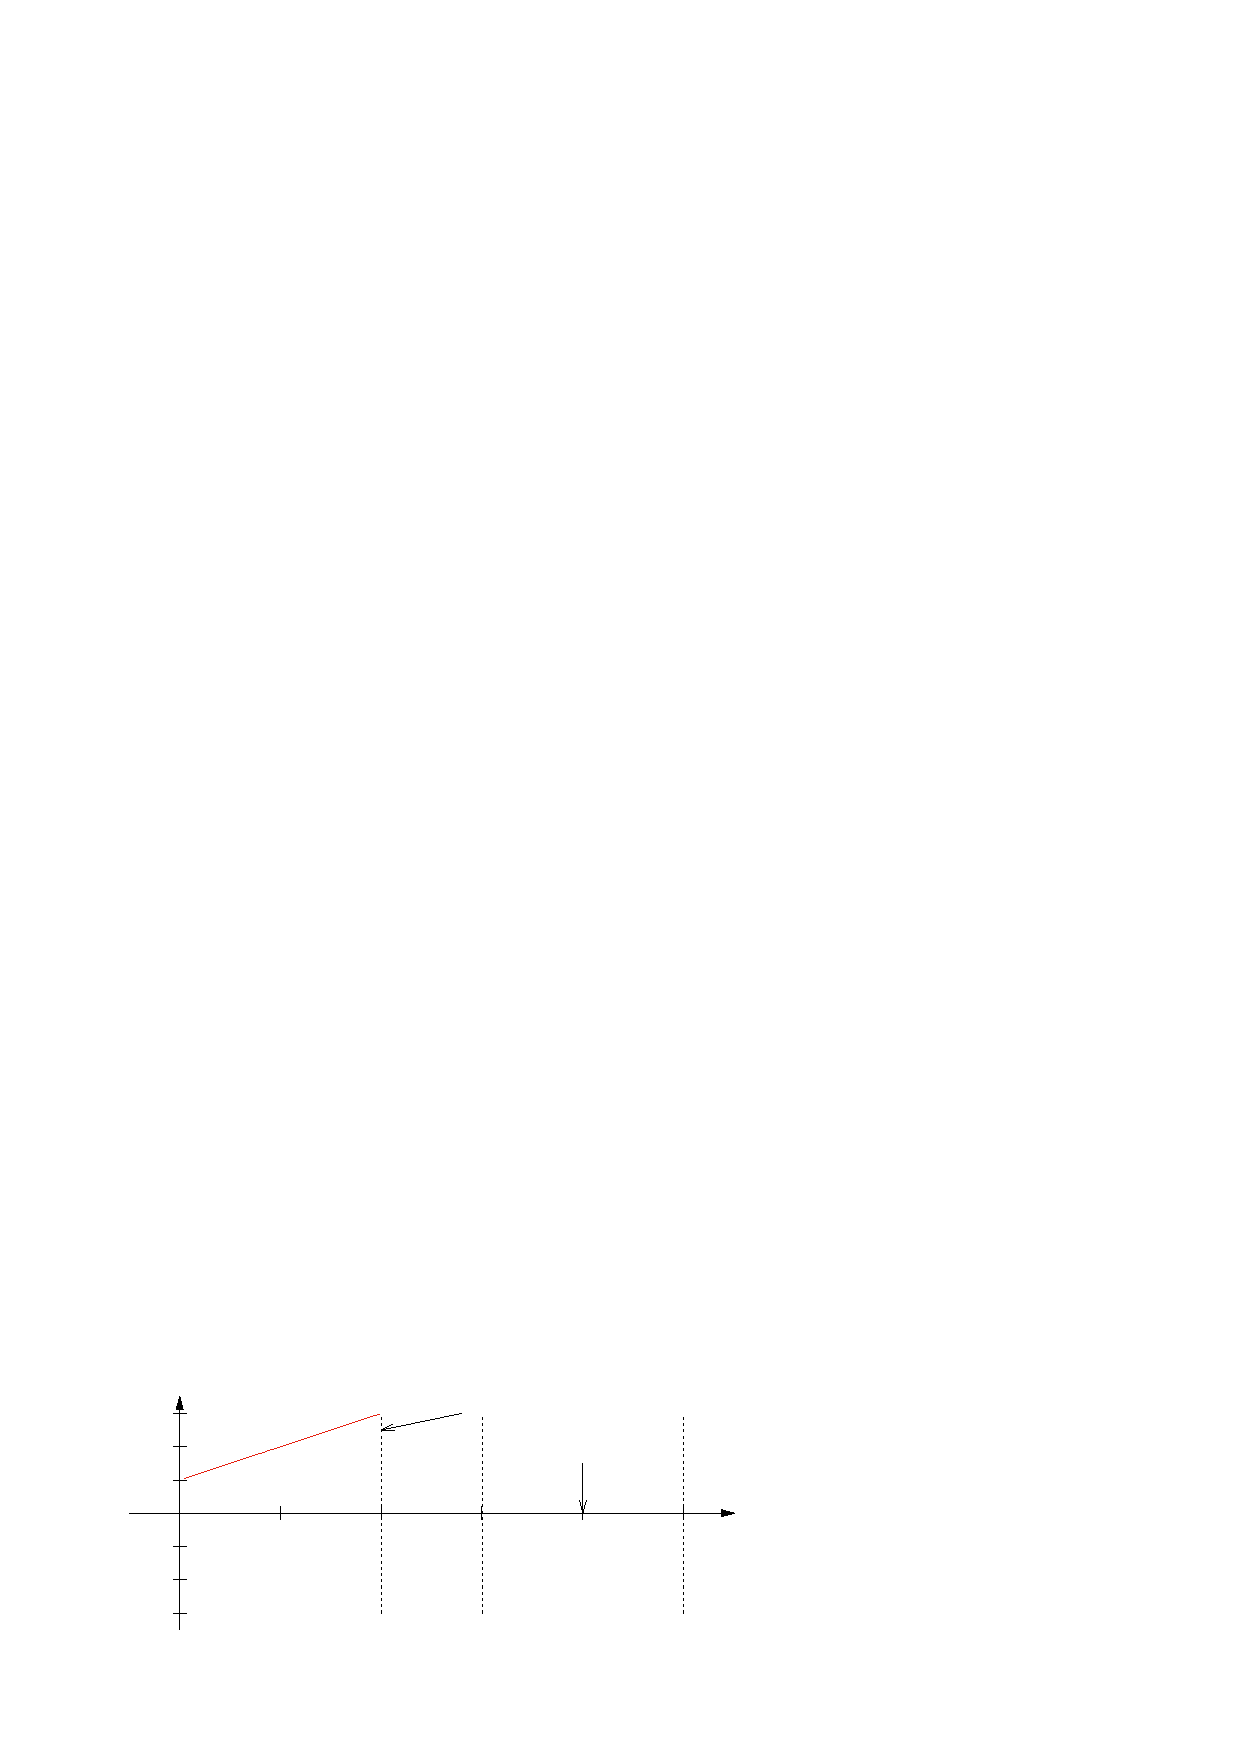
\includegraphics[width={316.80bp},height={129.50bp}]{figura_01_07}}%
    \gplfronttext
  \end{picture}%
\endgroup

    \end{figure}
    \begin{itemize}
    \item Debe existir un numero finito de discontinuidades (en 1 periodo).
    \item Debe existir un numero finito de extremos relativos (en 1 periodo).
    \end{itemize}
\item La integral $\int_0^T|f(t)|\,dt<\infty$ debe ser finita.
\end{itemize}

\textbf{Ejemplo}:
\begin{equation*}
    f(t)=\tan(t);\quad\,0<t<\pi;\quad\,T=\pi
\end{equation*}
\begin{figure}[H]
    \centering
    % GNUPLOT: LaTeX picture with Postscript
\begingroup
  \makeatletter
  \providecommand\color[2][]{%
    \GenericError{(gnuplot) \space\space\space\@spaces}{%
      Package color not loaded in conjunction with
      terminal option `colourtext'%
    }{See the gnuplot documentation for explanation.%
    }{Either use 'blacktext' in gnuplot or load the package
      color.sty in LaTeX.}%
    \renewcommand\color[2][]{}%
  }%
  \providecommand\includegraphics[2][]{%
    \GenericError{(gnuplot) \space\space\space\@spaces}{%
      Package graphicx or graphics not loaded%
    }{See the gnuplot documentation for explanation.%
    }{The gnuplot epslatex terminal needs graphicx.sty or graphics.sty.}%
    \renewcommand\includegraphics[2][]{}%
  }%
  \providecommand\rotatebox[2]{#2}%
  \@ifundefined{ifGPcolor}{%
    \newif\ifGPcolor
    \GPcolorfalse
  }{}%
  \@ifundefined{ifGPblacktext}{%
    \newif\ifGPblacktext
    \GPblacktexttrue
  }{}%
  % define a \g@addto@macro without @ in the name:
  \let\gplgaddtomacro\g@addto@macro
  % define empty templates for all commands taking text:
  \gdef\gplbacktext{}%
  \gdef\gplfronttext{}%
  \makeatother
  \ifGPblacktext
    % no textcolor at all
    \def\colorrgb#1{}%
    \def\colorgray#1{}%
  \else
    % gray or color?
    \ifGPcolor
      \def\colorrgb#1{\color[rgb]{#1}}%
      \def\colorgray#1{\color[gray]{#1}}%
      \expandafter\def\csname LTw\endcsname{\color{white}}%
      \expandafter\def\csname LTb\endcsname{\color{black}}%
      \expandafter\def\csname LTa\endcsname{\color{black}}%
      \expandafter\def\csname LT0\endcsname{\color[rgb]{1,0,0}}%
      \expandafter\def\csname LT1\endcsname{\color[rgb]{0,1,0}}%
      \expandafter\def\csname LT2\endcsname{\color[rgb]{0,0,1}}%
      \expandafter\def\csname LT3\endcsname{\color[rgb]{1,0,1}}%
      \expandafter\def\csname LT4\endcsname{\color[rgb]{0,1,1}}%
      \expandafter\def\csname LT5\endcsname{\color[rgb]{1,1,0}}%
      \expandafter\def\csname LT6\endcsname{\color[rgb]{0,0,0}}%
      \expandafter\def\csname LT7\endcsname{\color[rgb]{1,0.3,0}}%
      \expandafter\def\csname LT8\endcsname{\color[rgb]{0.5,0.5,0.5}}%
    \else
      % gray
      \def\colorrgb#1{\color{black}}%
      \def\colorgray#1{\color[gray]{#1}}%
      \expandafter\def\csname LTw\endcsname{\color{white}}%
      \expandafter\def\csname LTb\endcsname{\color{black}}%
      \expandafter\def\csname LTa\endcsname{\color{black}}%
      \expandafter\def\csname LT0\endcsname{\color{black}}%
      \expandafter\def\csname LT1\endcsname{\color{black}}%
      \expandafter\def\csname LT2\endcsname{\color{black}}%
      \expandafter\def\csname LT3\endcsname{\color{black}}%
      \expandafter\def\csname LT4\endcsname{\color{black}}%
      \expandafter\def\csname LT5\endcsname{\color{black}}%
      \expandafter\def\csname LT6\endcsname{\color{black}}%
      \expandafter\def\csname LT7\endcsname{\color{black}}%
      \expandafter\def\csname LT8\endcsname{\color{black}}%
    \fi
  \fi
    \setlength{\unitlength}{0.0500bp}%
    \ifx\gptboxheight\undefined%
      \newlength{\gptboxheight}%
      \newlength{\gptboxwidth}%
      \newsavebox{\gptboxtext}%
    \fi%
    \setlength{\fboxrule}{0.5pt}%
    \setlength{\fboxsep}{1pt}%
    \definecolor{tbcol}{rgb}{1,1,1}%
\begin{picture}(4320.00,4320.00)%
    \gplgaddtomacro\gplbacktext{%
      \csname LTb\endcsname%%
      \put(2040,192){\makebox(0,0)[r]{\strut{}}}%
      \put(2040,390){\makebox(0,0)[r]{\strut{}}}%
      \put(2040,589){\makebox(0,0)[r]{\strut{}}}%
      \put(2040,787){\makebox(0,0)[r]{\strut{}}}%
      \put(2040,985){\makebox(0,0)[r]{\strut{}}}%
      \put(2040,1184){\makebox(0,0)[r]{\strut{}}}%
      \put(2040,1382){\makebox(0,0)[r]{\strut{}}}%
      \put(2040,1580){\makebox(0,0)[r]{\strut{}}}%
      \put(2040,1779){\makebox(0,0)[r]{\strut{}}}%
      \put(2040,1977){\makebox(0,0)[r]{\strut{}}}%
      \put(2040,2176){\makebox(0,0)[r]{\strut{}}}%
      \put(2040,2374){\makebox(0,0)[r]{\strut{}}}%
      \put(2040,2572){\makebox(0,0)[r]{\strut{}}}%
      \put(2040,2771){\makebox(0,0)[r]{\strut{}}}%
      \put(2040,2969){\makebox(0,0)[r]{\strut{}}}%
      \put(2040,3167){\makebox(0,0)[r]{\strut{}}}%
      \put(2040,3366){\makebox(0,0)[r]{\strut{}}}%
      \put(2040,3564){\makebox(0,0)[r]{\strut{}}}%
      \put(2040,3762){\makebox(0,0)[r]{\strut{}}}%
      \put(2040,3961){\makebox(0,0)[r]{\strut{}}}%
      \put(2040,4159){\makebox(0,0)[r]{\strut{}}}%
      \put(511,1953){\makebox(0,0){\strut{}}}%
      \put(1052,1953){\makebox(0,0){\strut{}}}%
      \put(1594,1953){\makebox(0,0){\strut{}}}%
      \put(2136,1953){\makebox(0,0){\strut{}}}%
      \put(2677,1953){\makebox(0,0){\strut{}}}%
      \put(3219,1953){\makebox(0,0){\strut{}}}%
      \put(3760,1953){\makebox(0,0){\strut{}}}%
      \csname LTb\endcsname%%
      \put(4302,2176){\makebox(0,0)[l]{\strut{}$t$}}%
      \put(2015,4357){\makebox(0,0)[l]{\strut{}$f(t)$}}%
      \put(2574,1878){\makebox(0,0)[l]{\strut{}$\frac{\pi}{2}$}}%
      \put(3115,1878){\makebox(0,0)[l]{\strut{}$\pi$}}%
    }%
    \gplgaddtomacro\gplfronttext{%
    }%
    \gplbacktext
    \put(0,0){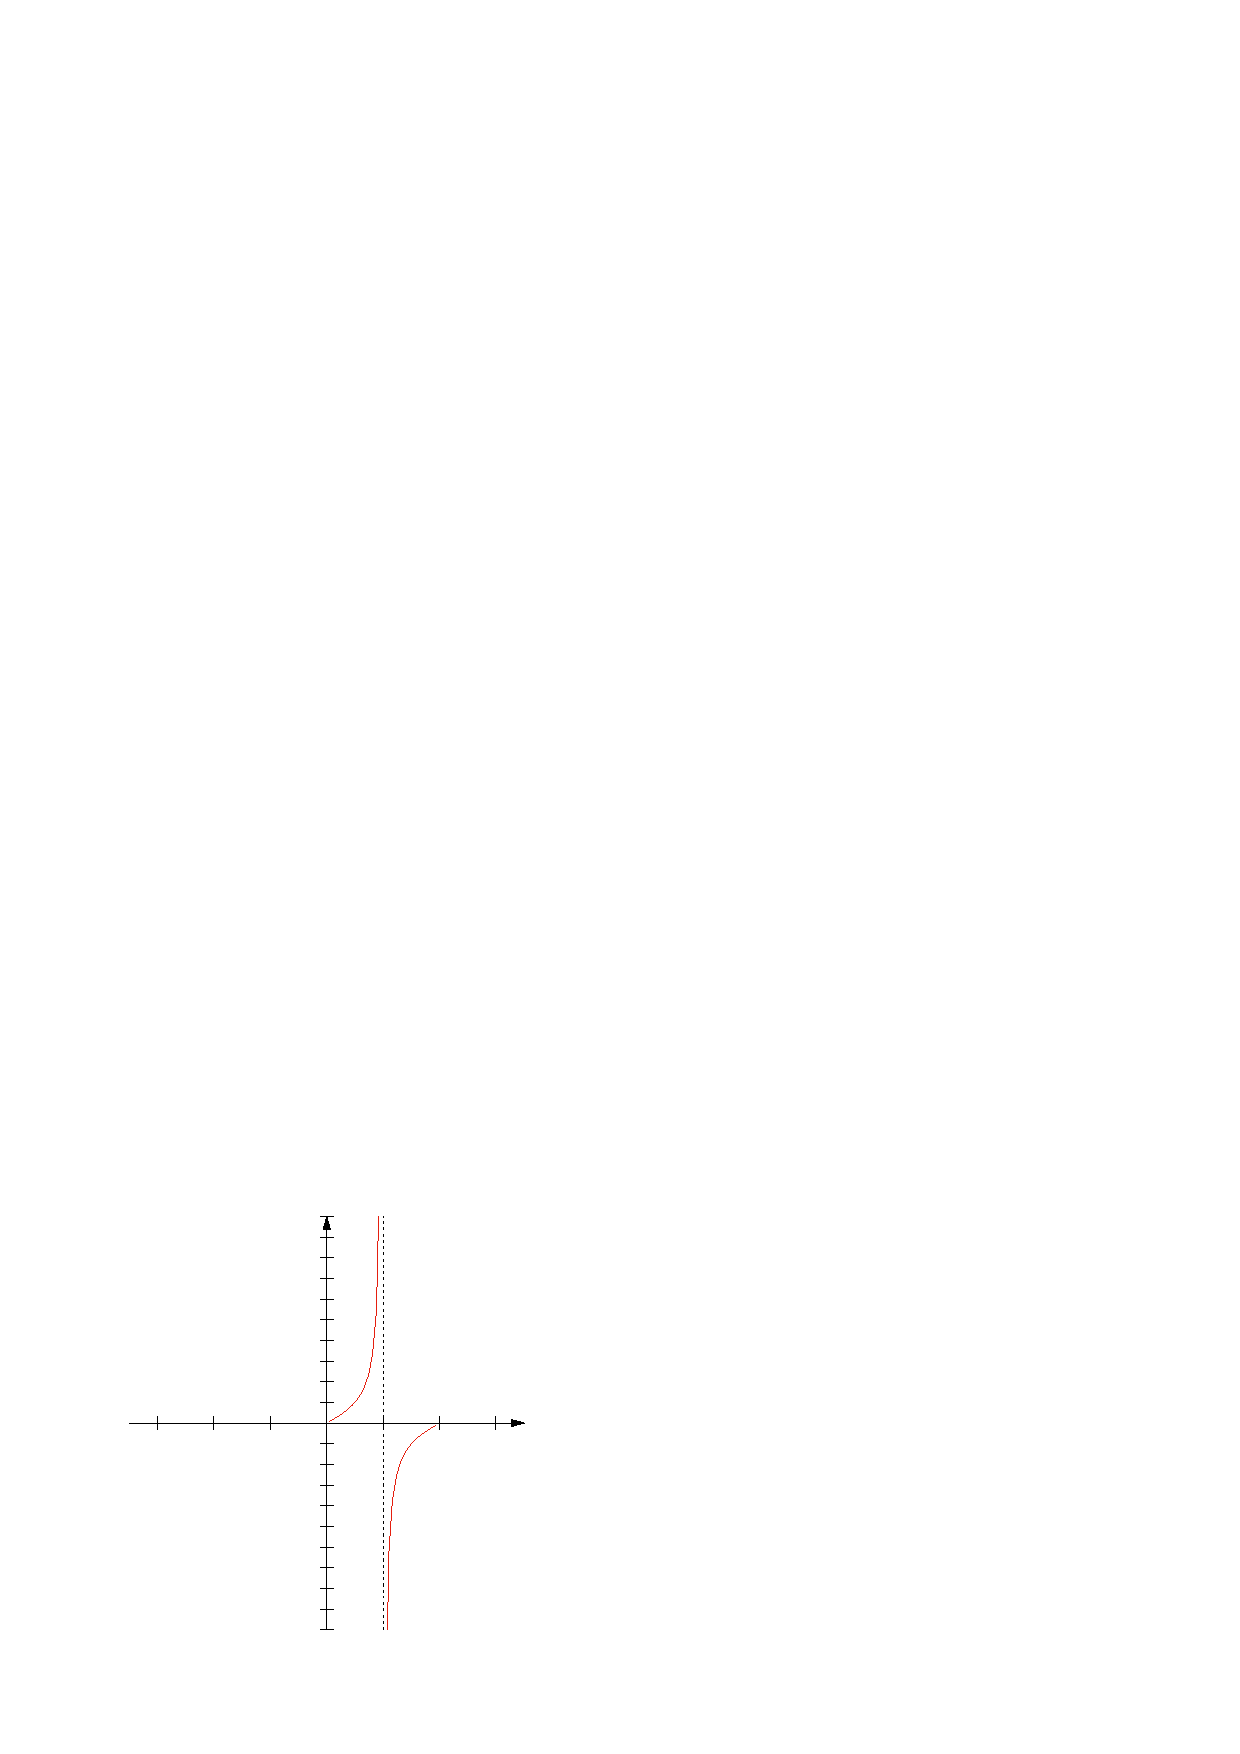
\includegraphics[width={216.00bp},height={216.00bp}]{figura_01_08}}%
    \gplfronttext
  \end{picture}%
\endgroup

\end{figure}
\begin{equation*}
    \int_0^\pi|\tan(t)|\,dt\rightarrow\infty
\end{equation*}
\begin{equation*}
    t=\frac{\pi}{2}:|\tan(t)|\rightarrow\infty
\end{equation*}
\\
\begin{equation*}
    \therefore\,\text{Esta función no tiene serie de \emph{Fourier}.}
\end{equation*}

\section{Evaluación de los coeficientes de \emph{Fourier}}
\begin{equation*}
    f(t)=\frac{a_0}{2}+
    \sum_{n=1}^{\infty}[a_n\cos(n\omega_0\,t)+b_n\sen(n\omega_0\,t)]
\end{equation*}

Integrando ambas partes:
\begin{equation*}
\begin{split}
    \int_{0}^{T}f(t)\,dt
        &=\int_{0}^{T}\frac{a_0}{2}\,dt+
          \sum_{n=1}^{\infty}\left[\int_{0}^{T}a_n\cos(n\omega_0\,t)\,dt+
          \int_{0}^{T}b_n\sen(n\omega_0\,t)\,dt\right]\\
        &=\frac{a_0}{2}t\Biggr|_{0}^{T}\\
        &=\frac{a_0}{2}T\\
\end{split}
\end{equation*}
\begin{equation}
    a_0=\frac{2}{T}\int_{0}^{T}f(t)\,dt
\end{equation}

Para calcular ``$a_n$'' multiplicamos por $\cos(m\omega_0\,t);m\in\mathbb{N}$ e
integramos en 1 periodo.
\begin{equation*}
\begin{split}
    \int_{0}^{T}f(t)\cos(m\omega_0\,t)\,dt
        &=\int_{0}^{T}\frac{a_0}{2}\cos(m\omega_0\,t)\,dt\\
        &+\sum_{n=1}^{\infty}\left[
          \int_{0}^{T}a_n\cos(n\omega_0\,t)\cos(m\omega_0\,t)\,dt+
          \int_{0}^{T}b_n\sen(n\omega_0\,t)\cos(m\omega_0\,t)\,dt\right]\\
        &=0+\sum_{n=1}^{\infty}\left[
          \int_{0}^{T}a_n\cos(n\omega_0\,t)\cos(m\omega_0\,t)\,dt+0\right]\\
\end{split}
\end{equation*}

Para $n\neq m$ todos los elementos de la sumatoria serán igual a $0$.
Por tanto:
\begin{equation*}
\begin{split}
    \int_{0}^{T}f(t)\cos(n\omega_0\,t)\,dt
        &=\int_{0}^{T}a_n\cos^2(n\omega_0\,t)\,dt\\
        &=a_n\frac{T}{2}\\
\end{split}
\end{equation*}
\begin{equation}
    a_n=\frac{2}{T}\int_{0}^{T}f(t)\cos(n\omega_0\,t)\,dt
\end{equation}

Para calcular ``$b_n$'' multiplicamos por $\sen(m\omega_0\,t);m\in\mathbb{N}$ e
integramos en 1 periodo.
\begin{equation*}
\begin{split}
    \int_{0}^{T}f(t)\sen(m\omega_0\,t)\,dt
        &=\int_{0}^{T}\frac{a_0}{2}\sen(m\omega_0\,t)\,dt\\
        &+\sum_{n=1}^{\infty}\left[
          \int_{0}^{T}a_n\cos(n\omega_0\,t)\sen(m\omega_0\,t)\,dt+
          \int_{0}^{T}b_n\sen(n\omega_0\,t)\sen(m\omega_0\,t)\,dt\right]\\
        &=0+\sum_{n=1}^{\infty}\left[
          0+\int_{0}^{T}b_n\sen(n\omega_0\,t)\sen(m\omega_0\,t)\,dt\right]\\
\end{split}
\end{equation*}

Para $n\neq\,m$ todos los elementos de la sumatoria serán igual a $0$.
Por tanto:
\begin{equation*}
\begin{split}
    \int_{0}^{T}f(t)\sen(n\omega_0\,t)\,dt
        &=\int_{0}^{T}b_n\sen^2(n\omega_0\,t)\,dt\\
        &=b_n\,\frac{T}{2}\\
\end{split}
\end{equation*}
\begin{equation}
    b_n=\frac{2}{T}\int_{0}^{T}f(t)\sen(n\omega_0\,t)\,dt
\end{equation}

\section{Formulas para las series de \emph{Fourier}}
\begin{equation*}
    \sen(\pi\,n)=0;\quad\,n\in\mathbb{N}
\end{equation*}
\begin{equation*}
    \cos(\pi\,n)={(-1)}^n;\quad\,n\in\mathbb{N}
\end{equation*}
\begin{equation*}
    \sen(2\pi\,n)=0;\quad\,n\in\mathbb{N}
\end{equation*}
\begin{equation*}
    \cos(2\pi\,n)=1;\quad\,n\in\mathbb{N}
\end{equation*}
\begin{equation*}
    \int\,\sen(at)\,dt=-\frac{\cos(at)}{a}
\end{equation*}
\begin{equation*}
    \int\,\cos(at)\,dt=\frac{\sen(at)}{a}
\end{equation*}
\begin{equation*}
    \int\,t\sen(at)\,dt=-\frac{t}{a}\cos(at)+\frac{1}{a^2}\sen(at)
\end{equation*}
\begin{equation*}
    \int\,t\cos(at)\,dt=\frac{t}{a}\sen(at)+\frac{1}{a^2}\cos(at)
\end{equation*}
\begin{equation*}
    \int\,{e}^{at}\,dt=\frac{1}{a}e^{at}
\end{equation*}
\begin{equation*}
    \int\,t\,{e}^{at}\,dt=\frac{t}{a}\,{e}^{at}-\frac{1}{a^2}{e}^{at}
\end{equation*}


\chapter{Ecuaciones de \emph{Lagrange} para una partícula}

\section{Introducción}

Ecuación de \emph{Lagrange}:

\begin{equation*}
    \frac{d}{dt}\left(\frac{\partial T}{\partial \dot{q}_r}\right)-
    \frac{\partial T}{\partial q_r}=F_{q_r}
\end{equation*}

Principio de \emph{d'Alembert}:

\begin{equation*}
    m(\ddot{x}\delta x+\ddot{y}\delta y+\ddot{z}\delta z)=
    F_x\delta x+F_y\delta y+F_z\delta z
\end{equation*}

\section{Deducción de la ecuación de \emph{Lagrange}}

\begin{equation*}
    \begin{cases}
        x=x(q_1,q_2)\\
        y=y(q_1,q_2)\\
        z=z(q_1,q_2)
    \end{cases}
\end{equation*}

\begin{equation*}
    \delta_x=\frac{\partial x}{\partial q_1}\delta q_1+
             \frac{\partial x}{\partial q_2}\delta q_2
\end{equation*}
\begin{equation*}
    \delta_y=\frac{\partial y}{\partial q_1}\delta q_1+
             \frac{\partial y}{\partial q_2}\delta q_2
\end{equation*}
\begin{equation*}
    \delta_z=\frac{\partial z}{\partial q_1}\delta q_1+
             \frac{\partial z}{\partial q_2}\delta q_2
\end{equation*}

\begin{equation*}
\begin{split}
    m\left(
        \ddot{x}\left(
            \frac{\partial x}{\partial q_1}\delta q_1+
            \frac{\partial x}{\partial q_2}\delta q_2
        \right)+
        \ddot{y}\left(
            \frac{\partial y}{\partial q_1}\delta q_1+
            \frac{\partial y}{\partial q_2}\delta q_2
        \right)+
        \ddot{z}\left(
            \frac{\partial z}{\partial q_1}\delta q_1+
            \frac{\partial z}{\partial q_2}\delta q_2
        \right)
    \right)=\\
    F_x\left(
        \frac{\partial x}{\partial q_1}\delta q_1+
        \frac{\partial x}{\partial q_2}\delta q_2
    \right)+
    F_y\left(
        \frac{\partial y}{\partial q_1}\delta q_1+
        \frac{\partial y}{\partial q_2}\delta q_2
    \right)+
    F_z\left(
        \frac{\partial z}{\partial q_1}\delta q_1+
        \frac{\partial z}{\partial q_2}\delta q_2
    \right)
\end{split}
\end{equation*}

\begin{equation*}
\begin{split}
    m\left(
        \ddot{x}\frac{\partial x}{\partial q_1}\delta q_1+
        \ddot{y}\frac{\partial y}{\partial q_1}\delta q_1+
        \ddot{z}\frac{\partial z}{\partial q_1}\delta q_1
    \right)+
    m\left(
        \ddot{x}\frac{\partial x}{\partial q_2}\delta q_2+
        \ddot{y}\frac{\partial y}{\partial q_2}\delta q_2+
        \ddot{z}\frac{\partial z}{\partial q_2}\delta q_2
    \right)=\\
    \left(
        F_x\frac{\partial x}{\partial q_1}\delta q_1+
        F_y\frac{\partial y}{\partial q_1}\delta q_1+
        F_z\frac{\partial z}{\partial q_1}\delta q_1
    \right)+
    \left(
        F_x\frac{\partial x}{\partial q_2}\delta q_2+
        F_y\frac{\partial y}{\partial q_2}\delta q_2+
        F_z\frac{\partial z}{\partial q_2}\delta q_2
    \right)
\end{split}
\end{equation*}

\begin{equation*}
\begin{split}
    m\left(
        \left(
            \ddot{x}\frac{\partial x}{\partial q_1}+
            \ddot{y}\frac{\partial y}{\partial q_1}+
            \ddot{z}\frac{\partial z}{\partial q_1}
        \right)\delta q_1
    \right)+
    m\left(
        \left(
            \ddot{x}\frac{\partial x}{\partial q_2}+
            \ddot{y}\frac{\partial y}{\partial q_2}+
            \ddot{z}\frac{\partial z}{\partial q_2}
        \right)\delta q_2
    \right)=\\
    \left(
        F_x\frac{\partial x}{\partial q_1}+
        F_y\frac{\partial y}{\partial q_1}+
        F_z\frac{\partial z}{\partial q_1}
    \right)\delta q_1+
    \left(
        F_x\frac{\partial x}{\partial q_2}+
        F_y\frac{\partial y}{\partial q_2}+
        F_z\frac{\partial z}{\partial q_2}
    \right)\delta q_2
\end{split}
\end{equation*}

Si $q_2=0$:

\begin{equation}
    m\left(
        \left(
            \ddot{x}\frac{\partial x}{\partial q_1}+
            \ddot{y}\frac{\partial y}{\partial q_1}+
            \ddot{z}\frac{\partial z}{\partial q_1}
        \right)\delta q_1
    \right)=
    \left(
        F_x\frac{\partial x}{\partial q_1}+
        F_y\frac{\partial y}{\partial q_1}+
        F_z\frac{\partial z}{\partial q_1}
    \right)\delta q_1
    \label{general1}
\end{equation}

Sabiendo que por la regla de la cadena:

\begin{equation*}
    \frac{d}{dt}\left(\dot{x}\frac{\partial x}{\partial q_1}\right)=
    \ddot{x}\frac{\partial x}{\partial q_1}+
    \dot{x}\frac{d}{dt}\left(\frac{\partial x}{\partial q_1}\right)
\end{equation*}

\begin{equation}
    \ddot{x}\frac{\partial x}{\partial q_1}=
    \frac{d}{dt}\left(\dot{x}\frac{\partial x}{\partial q_1}\right)-
    \dot{x}\frac{d}{dt}\left(\frac{\partial x}{\partial q_1}\right)
    \label{base}
\end{equation}

Por otro lado, derivando $x=x(q_1,q_2)$ con respecto al tiempo:

\begin{equation*}
    \dot{x}=\frac{\partial x}{\partial q_1}\dot{q_1}+
            \frac{\partial x}{\partial q_2}\dot{q_2}
\end{equation*}

Y derivando con respecto a $\dot{q_1}$:

\begin{equation}
    \frac{\partial \dot{x}}{\partial \dot{q_1}}=\frac{\partial x}{\partial q_1}
    \label{primerTermino}
\end{equation}

Por otro lado:

\begin{equation}
    \frac{d}{dt}\left(\frac{\partial x}{\partial q_1}\right)=
    \frac{\partial}{\partial q_1}\left(\frac{dx}{dt}\right)=
    \frac{\partial \dot{x}}{\partial q_1}
    \label{segundoTermino}
\end{equation}

Combinando~\ref{primerTermino} y~\ref{segundoTermino} en~\ref{base}, se obtiene:

\begin{equation}
    \ddot{x}\frac{\partial x}{\partial q_1}=
    \frac{d}{dt}\left(\dot{x}\frac{\partial \dot{x}}{\partial \dot{q_1}}\right)-
    \dot{x}\frac{\partial \dot{x}}{\partial q_1}
    \label{condensado}
\end{equation}

Por otro lado:

\begin{equation}
    \frac{\partial}{\partial q_1}\left(\frac{1}{2}\dot{x}^2\right)=
    \frac{1}{2}2\dot{x}\frac{\partial\dot{x}}{\partial q_1}=
    \dot{x}\frac{\partial\dot{x}}{\partial q_1}
    \label{cinetica1}
\end{equation}

\begin{equation}
    \frac{\partial}{\partial \dot{q}_1}\left(\frac{1}{2}\dot{x}^2\right)=
    \frac{1}{2}2\dot{x}\frac{\partial\dot{x}}{\partial \dot{q}_1}=
    \dot{x}\frac{\partial\dot{x}}{\partial \dot{q}_1}
    \label{cinetica2}
\end{equation}

Combinando~\ref{cinetica1} y~\ref{cinetica2} en~\ref{condensado}:

\begin{equation}
    \ddot{x}\frac{\partial x}{\partial q_1}=
    \frac{d}{dt}\left(\frac{\partial}{\partial \dot{q}_1}
        \left(\frac{1}{2}\dot{x}^2\right)
    \right)-
    \frac{\partial}{\partial q_1}\left(\frac{1}{2}\dot{x}^2\right)
    \label{condensado2}
\end{equation}

Sustituyendo~\ref{condensado2}, agregando las relaciones para $y$ y $z$ y
reagrupando términos en~\ref{general1}:

\begin{equation*}
\begin{split}
    \left[
        \frac{d}{dt}\left(
            \frac{\partial}{\partial\dot{q}_1}\left(
                \frac{1}{2}m(\dot{x}^2+\dot{y}^2+\dot{z}^2)
            \right)
        \right)-
        \frac{\partial}{\partial q_1}\left(
            \frac{1}{2}m(\dot{x}^2+\dot{y}^2+\dot{z}^2)
        \right)
    \right]\delta q_1=\\
    \left(
        F_x\frac{\partial x}{\partial q_1}+
        F_y\frac{\partial y}{\partial q_1}+
        F_z\frac{\partial z}{\partial q_1}
    \right)\delta q_1
\end{split}
\end{equation*}

Considerando que $\frac{1}{2}m(\dot{x}^2+\dot{y}^2+\dot{z}^2)$ representa la
energía cinética ($T$), finalmente se obtiene:

\begin{equation*}
    \frac{d}{dt}\left(
        \frac{\partial T}{\partial\dot{q}_1}
    \right)-
    \frac{\partial T}{\partial q_1}=
    F_x\frac{\partial x}{\partial q_1}+
    F_y\frac{\partial y}{\partial q_1}+
    F_z\frac{\partial z}{\partial q_1}
    \label{lagrange}
\end{equation*}

\section{Determinación de la aceleración}
La componente $a'$ del vector aceleración $a$, sobre una linea cuyos cosenos
directores son: $l$, $m$, $n$, esta dada por:

\begin{equation*}
    a'=\ddot{x}l+\ddot{y}m+\ddot{z}n
\end{equation*}

Si debe hallarse $a'$ en la dirección de la tangente a una curva en el espacio
en un punto $p$ determinado.

\begin{align*}
    l&=\frac{dx}{ds}; & m&=\frac{dy}{ds}; & n&=\frac{dz}{ds}
\end{align*}
\begin{equation*}
    ds^2=dx^2+dy^2+dz^2
\end{equation*}

Entonces, partiendo de las ecuaciones de la curva en el espacio, puede hallarse
$l$, $m$, $n$, supóngase que se desea determinar una expresión general para la
componente de la aceleración en la dirección de la tangente a la coordenada
$q_1$, teniendo en cuenta que las coordenadas generalizadas $q_1$, $q_2$, $q_3$
se relacionan con las rectangulares por medio de:

\begin{align*}
    x&=x(q_1,q_2,q_3,t); & y&=y(q_1,q_2,q_3,t); & z=z(q_1,q_2,q_3,t)
\end{align*}

La linea coordenada de $q_1$ se determina haciendo que permanezcan constantes
$q_2$, $q_3$, $t$. En forma semejante se obtienen las lineas coordenadas de
$q_2$ y $q_3$. Tomando las derivadas se obtienen:

\begin{align*}
    dx&=\frac{\partial x}{\partial q_1}dq_1; &
    dy&=\frac{\partial y}{\partial q_1}dq_1; &
    dz&=\frac{\partial z}{\partial q_1}dq_1
\end{align*}

Por tanto:

\begin{equation*}
    {ds}^2=\left[
        {\left(\frac{\partial x}{\partial q_1}\right)}^2+
        {\left(\frac{\partial y}{\partial q_1}\right)}^2+
        {\left(\frac{\partial z}{\partial q_1}\right)}^2
    \right] dq^2_1
\end{equation*}

En donde $ds$ es un elemento de longitud medido sobre la curva de $q$

\begin{equation*}
    l_1=\frac{dx}{dq_1{\left[
            {\left(\frac{\partial x}{\partial q_1}\right)}^2+
            {\left(\frac{\partial y}{\partial q_1}\right)}^2+
            {\left(\frac{\partial z}{\partial q_1}\right)}^2
        \right]}^\frac{1}{2}}
       =\frac{1}{h_1}\frac{\partial x}{\partial q_1}
\end{equation*}

En donde el significado de $h_1$ es claro, y donde se ha escrito $dx/dq_1$ como
$\partial x/\partial q_1$ puesto que $q_2$, $q_3$ y $t$ se consideran todavía
constantes. En forma semejante
$m_1=\frac{1}{h_1}\frac{\partial y}{\partial q_1}$ y
$n_1=\frac{1}{h_1}\frac{\partial y}{\partial q_1}$. Igualmente los cosenos
directores de la tangente a la curva coordenada de $q_2$, son:

\begin{align*}
    l_2&=\frac{1}{h_2}\frac{\partial x}{\partial q_2}; &
    m_2&=\frac{1}{h_2}\frac{\partial y}{\partial q_2}; &
    n_2&=\frac{1}{h_2}\frac{\partial z}{\partial q_2};
\end{align*}

Designando $a'$ como $a_{q_1}$ la ecuación se convierte en:

\begin{equation*}
    a'=a_{q_1}=\frac{1}{h_1}\left(
        \ddot{x}\frac{\partial x}{\partial q_1}+
        \ddot{y}\frac{\partial y}{\partial q_1}+
        \ddot{z}\frac{\partial z}{\partial q_1}
    \right)
\end{equation*}

Teniendo en cuenta las etapas que condujeron al miembro izquierdo de la ecuación
de \emph{Lagrange}, evidentemente puede escribirse en la siguiente forma:

\begin{equation*}
    a_{q_r}=\frac{1}{h_{q_r}}\left[
        \frac{d}{dt}\left(\frac{\partial T'}{\partial\dot{q}_r}\right)-
        \frac{\partial T'}{\partial q_r}
    \right]
\end{equation*}
\begin{equation*}
    T'=\frac{1}{2}v^2=\frac{1}{2}(\dot{x}^2+\dot{y}^2+\dot{z}^2)
\end{equation*}

\section{Ejemplos}

\subsection{Ejemplo 1}
Determinar las ecuaciones de movimiento de una partícula que se mueve por acción
de una fuerza $F$. Suponer que el movimiento es en un plano.

\subsection{Ejemplo 2}
Determinar las ecuaciones de movimiento de una partícula de masa $m$ por la
acción de una fuerza, la misma que tiene movimiento lineal, y angular, la fuerza
que hace posible el movimiento es $F$.

\subsection{Ejemplo 3}
3.5. Una cuenta puede moverse restringida a una espiral cónica lisa. Suponiendo
que $\rho=az$ y que $\phi=-bz$, en donde $a$ y $b$ son constantes, demostrar que
la ecuación del movimiento es:

\begin{equation*}
    \ddot{z}(a^2+1+a^2b^2z^2)+a^2b^2z\dot{z}^2=-g
\end{equation*}

\subsection{Ejemplo 4}
3.7. La masa $m$ del péndulo esta suspendida por medio de un hilo inextensible
del punto $p$. Este punto puede moverse libremente sobre una horizontal bajo la
acción de los resortes, los cuales tienen una constante $k$. Despreciando la
masa de los resortes, demostrar que el péndulo oscila con un periodo igual a:

\begin{equation*}
    P=2r\sqrt{\frac{mg+2kr}{2kg}}
\end{equation*}

\subsection{Ejemplo 5}
Determinar la frecuencia de las pequeñas oscilaciones de un péndulo envolvente
en el campo gravitacional. El radio $r$ del cilindro y la longitud libre $l_0$
de la soga en su posición de equilibrio son datos conocidos.

\subsection{Ejemplo 6}
Un segmento cilíndrico se balancea sobre un plano rugoso por la acción del campo
gravitacional. Determinar el periodo de oscilación, los datos son: la masa $m$,
el momento inercial $I_s$ con respecto al centro de gravedad y la excentricidad
del centro de gravedad $e$.

\subsection{Ejemplo 7}
3.1. Suponiendo que el movimiento está restringido al plano $Q_1 Q_2$ y que la
gravedad actúa en la dirección negativa del eje vertical $Y$, establézcanse las
ecuaciones del movimiento de un proyectil en función de las coordenadas $q_1$ y
$q_2$.


\subsection{Ejemplo 8}
Determinar las ecuaciones de aceleración para una partícula en coordenadas
esféricas.

\subsection{Ejemplo 9}
Determinar las ecuaciones de aceleración para una partícula en coordenadas
polares.

\subsection{Ejemplo 10}
3.16. Un disco pesado uniforme, de radio $R$, rueda por un plano inclinado sin
resbalar. Los ejes $X$ y $Y$ están adheridos a la superficie del disco con el
origen en el centro. Una partícula de masa $m$ puede moverse libremente en el
plano del disco bajo la acción de la gravedad y de un sistema de resortes cuyos
detalles no es necesario especificar. Por consideraciones elementales puede
decirse que despreciando  la pequeña masa de la partícula, el centro del disco
se mueve con aceleración lineal $a=\frac{2}{3}g\sen(\alpha)$, en donde $\alpha$
es el ángulo de inclinación del plano. Demostrar que la energía cinética de la
partícula en coordenadas polares $r$ y $\theta$ ($\theta$ medido a partir del
eje $X$ adherido al disco) esta dada por: ($\beta$ se mide entre $X$ y una recta
fija normal al plano inclinado)

\begin{equation*}
    T=\frac{1}{2}m[
        a^2t^2+
        \dot{r}^2+
        r^2{(\dot{\beta}-\dot{\theta})}^2+
        2at\dot{r}\sen(\beta-\theta)+
        2atr(\dot{\beta}-\dot{\theta})\cos(\beta-\theta)
    ]
\end{equation*}

en donde $\dot{\beta}=(a/R)t$.

\subsection{Ejemplo 11}
3.21. Un alambre rígido parabólico que gira de una cierta manera alrededor del
eje $Z_2$ al mismo tiempo que la plataforma a la cual se halla adherido el
sistema $X_2$, $Y_2$, $Z_2$ se mueve con aceleración constante $a$, paralela al
eje $Y_1$. La cuenta de masa $m$ puede deslizarse a lo largo del alambre liso
bajo la fuerza de la gravedad. (a) Demostrar que:

\begin{equation*}
    T=\frac{1}{2}m[
        \dot{r}^2+
        r^2\dot{\phi}^2+
        a^2t^2+
        2\dot{r}at\sen(\phi)+
        2r\dot{\phi}at\cos(\phi)+
        4b^2r^2\dot{r}^2
    ]
\end{equation*}

Suponiendo $\dot{\phi}=\omega=\text{constante}$, plantear la ecuación del
movimiento correspondiente a $r$, y demostrar que:

\begin{equation*}
    F_r=-2mgbr
\end{equation*}


\chapter{Serie compleja de \emph{Fourier} y espectros discretos de frecuencia}

\section{Números complejos}
\begin{figure}[H]
    \centering
    % GNUPLOT: LaTeX picture with Postscript
\begingroup
  \makeatletter
  \providecommand\color[2][]{%
    \GenericError{(gnuplot) \space\space\space\@spaces}{%
      Package color not loaded in conjunction with
      terminal option `colourtext'%
    }{See the gnuplot documentation for explanation.%
    }{Either use 'blacktext' in gnuplot or load the package
      color.sty in LaTeX.}%
    \renewcommand\color[2][]{}%
  }%
  \providecommand\includegraphics[2][]{%
    \GenericError{(gnuplot) \space\space\space\@spaces}{%
      Package graphicx or graphics not loaded%
    }{See the gnuplot documentation for explanation.%
    }{The gnuplot epslatex terminal needs graphicx.sty or graphics.sty.}%
    \renewcommand\includegraphics[2][]{}%
  }%
  \providecommand\rotatebox[2]{#2}%
  \@ifundefined{ifGPcolor}{%
    \newif\ifGPcolor
    \GPcolorfalse
  }{}%
  \@ifundefined{ifGPblacktext}{%
    \newif\ifGPblacktext
    \GPblacktexttrue
  }{}%
  % define a \g@addto@macro without @ in the name:
  \let\gplgaddtomacro\g@addto@macro
  % define empty templates for all commands taking text:
  \gdef\gplbacktext{}%
  \gdef\gplfronttext{}%
  \makeatother
  \ifGPblacktext
    % no textcolor at all
    \def\colorrgb#1{}%
    \def\colorgray#1{}%
  \else
    % gray or color?
    \ifGPcolor
      \def\colorrgb#1{\color[rgb]{#1}}%
      \def\colorgray#1{\color[gray]{#1}}%
      \expandafter\def\csname LTw\endcsname{\color{white}}%
      \expandafter\def\csname LTb\endcsname{\color{black}}%
      \expandafter\def\csname LTa\endcsname{\color{black}}%
      \expandafter\def\csname LT0\endcsname{\color[rgb]{1,0,0}}%
      \expandafter\def\csname LT1\endcsname{\color[rgb]{0,1,0}}%
      \expandafter\def\csname LT2\endcsname{\color[rgb]{0,0,1}}%
      \expandafter\def\csname LT3\endcsname{\color[rgb]{1,0,1}}%
      \expandafter\def\csname LT4\endcsname{\color[rgb]{0,1,1}}%
      \expandafter\def\csname LT5\endcsname{\color[rgb]{1,1,0}}%
      \expandafter\def\csname LT6\endcsname{\color[rgb]{0,0,0}}%
      \expandafter\def\csname LT7\endcsname{\color[rgb]{1,0.3,0}}%
      \expandafter\def\csname LT8\endcsname{\color[rgb]{0.5,0.5,0.5}}%
    \else
      % gray
      \def\colorrgb#1{\color{black}}%
      \def\colorgray#1{\color[gray]{#1}}%
      \expandafter\def\csname LTw\endcsname{\color{white}}%
      \expandafter\def\csname LTb\endcsname{\color{black}}%
      \expandafter\def\csname LTa\endcsname{\color{black}}%
      \expandafter\def\csname LT0\endcsname{\color{black}}%
      \expandafter\def\csname LT1\endcsname{\color{black}}%
      \expandafter\def\csname LT2\endcsname{\color{black}}%
      \expandafter\def\csname LT3\endcsname{\color{black}}%
      \expandafter\def\csname LT4\endcsname{\color{black}}%
      \expandafter\def\csname LT5\endcsname{\color{black}}%
      \expandafter\def\csname LT6\endcsname{\color{black}}%
      \expandafter\def\csname LT7\endcsname{\color{black}}%
      \expandafter\def\csname LT8\endcsname{\color{black}}%
    \fi
  \fi
    \setlength{\unitlength}{0.0500bp}%
    \ifx\gptboxheight\undefined%
      \newlength{\gptboxheight}%
      \newlength{\gptboxwidth}%
      \newsavebox{\gptboxtext}%
    \fi%
    \setlength{\fboxrule}{0.5pt}%
    \setlength{\fboxsep}{1pt}%
    \definecolor{tbcol}{rgb}{1,1,1}%
\begin{picture}(2880.00,2880.00)%
    \gplgaddtomacro\gplbacktext{%
      \csname LTb\endcsname%%
      \put(614,192){\makebox(0,0)[r]{\strut{}}}%
      \put(614,697){\makebox(0,0)[r]{\strut{}}}%
      \put(614,1203){\makebox(0,0)[r]{\strut{}}}%
      \put(614,1708){\makebox(0,0)[r]{\strut{}}}%
      \put(614,2214){\makebox(0,0)[r]{\strut{}}}%
      \put(614,2719){\makebox(0,0)[r]{\strut{}}}%
      \put(240,474){\makebox(0,0){\strut{}}}%
      \put(710,474){\makebox(0,0){\strut{}}}%
      \put(1180,474){\makebox(0,0){\strut{}}}%
      \put(1651,474){\makebox(0,0){\strut{}}}%
      \put(2121,474){\makebox(0,0){\strut{}}}%
      \put(2591,474){\makebox(0,0){\strut{}}}%
      \csname LTb\endcsname%%
      \put(3061,697){\makebox(0,0)[l]{\strut{}$\mathbb{R}e$}}%
      \put(875,2845){\makebox(0,0)[l]{\strut{}$\mathbb{I}m$}}%
      \put(1886,2441){\makebox(0,0)[l]{\strut{}$z=a+jb$}}%
      \put(2074,521){\makebox(0,0)[l]{\strut{}$a$}}%
      \put(358,2239){\makebox(0,0)[l]{\strut{}$jb$}}%
      \put(1274,900){\makebox(0,0)[l]{\strut{}$\theta$}}%
    }%
    \gplgaddtomacro\gplfronttext{%
    }%
    \gplgaddtomacro\gplbacktext{%
      \csname LTb\endcsname%%
      \put(614,192){\makebox(0,0)[r]{\strut{}}}%
      \put(614,697){\makebox(0,0)[r]{\strut{}}}%
      \put(614,1203){\makebox(0,0)[r]{\strut{}}}%
      \put(614,1708){\makebox(0,0)[r]{\strut{}}}%
      \put(614,2214){\makebox(0,0)[r]{\strut{}}}%
      \put(614,2719){\makebox(0,0)[r]{\strut{}}}%
      \put(240,474){\makebox(0,0){\strut{}}}%
      \put(710,474){\makebox(0,0){\strut{}}}%
      \put(1180,474){\makebox(0,0){\strut{}}}%
      \put(1651,474){\makebox(0,0){\strut{}}}%
      \put(2121,474){\makebox(0,0){\strut{}}}%
      \put(2591,474){\makebox(0,0){\strut{}}}%
      \csname LTb\endcsname%%
      \put(3061,697){\makebox(0,0)[l]{\strut{}$\mathbb{R}e$}}%
      \put(875,2845){\makebox(0,0)[l]{\strut{}$\mathbb{I}m$}}%
      \put(1886,2441){\makebox(0,0)[l]{\strut{}$z=a+jb$}}%
      \put(2074,521){\makebox(0,0)[l]{\strut{}$a$}}%
      \put(358,2239){\makebox(0,0)[l]{\strut{}$jb$}}%
      \put(1274,900){\makebox(0,0)[l]{\strut{}$\theta$}}%
    }%
    \gplgaddtomacro\gplfronttext{%
    }%
    \gplbacktext
    \put(0,0){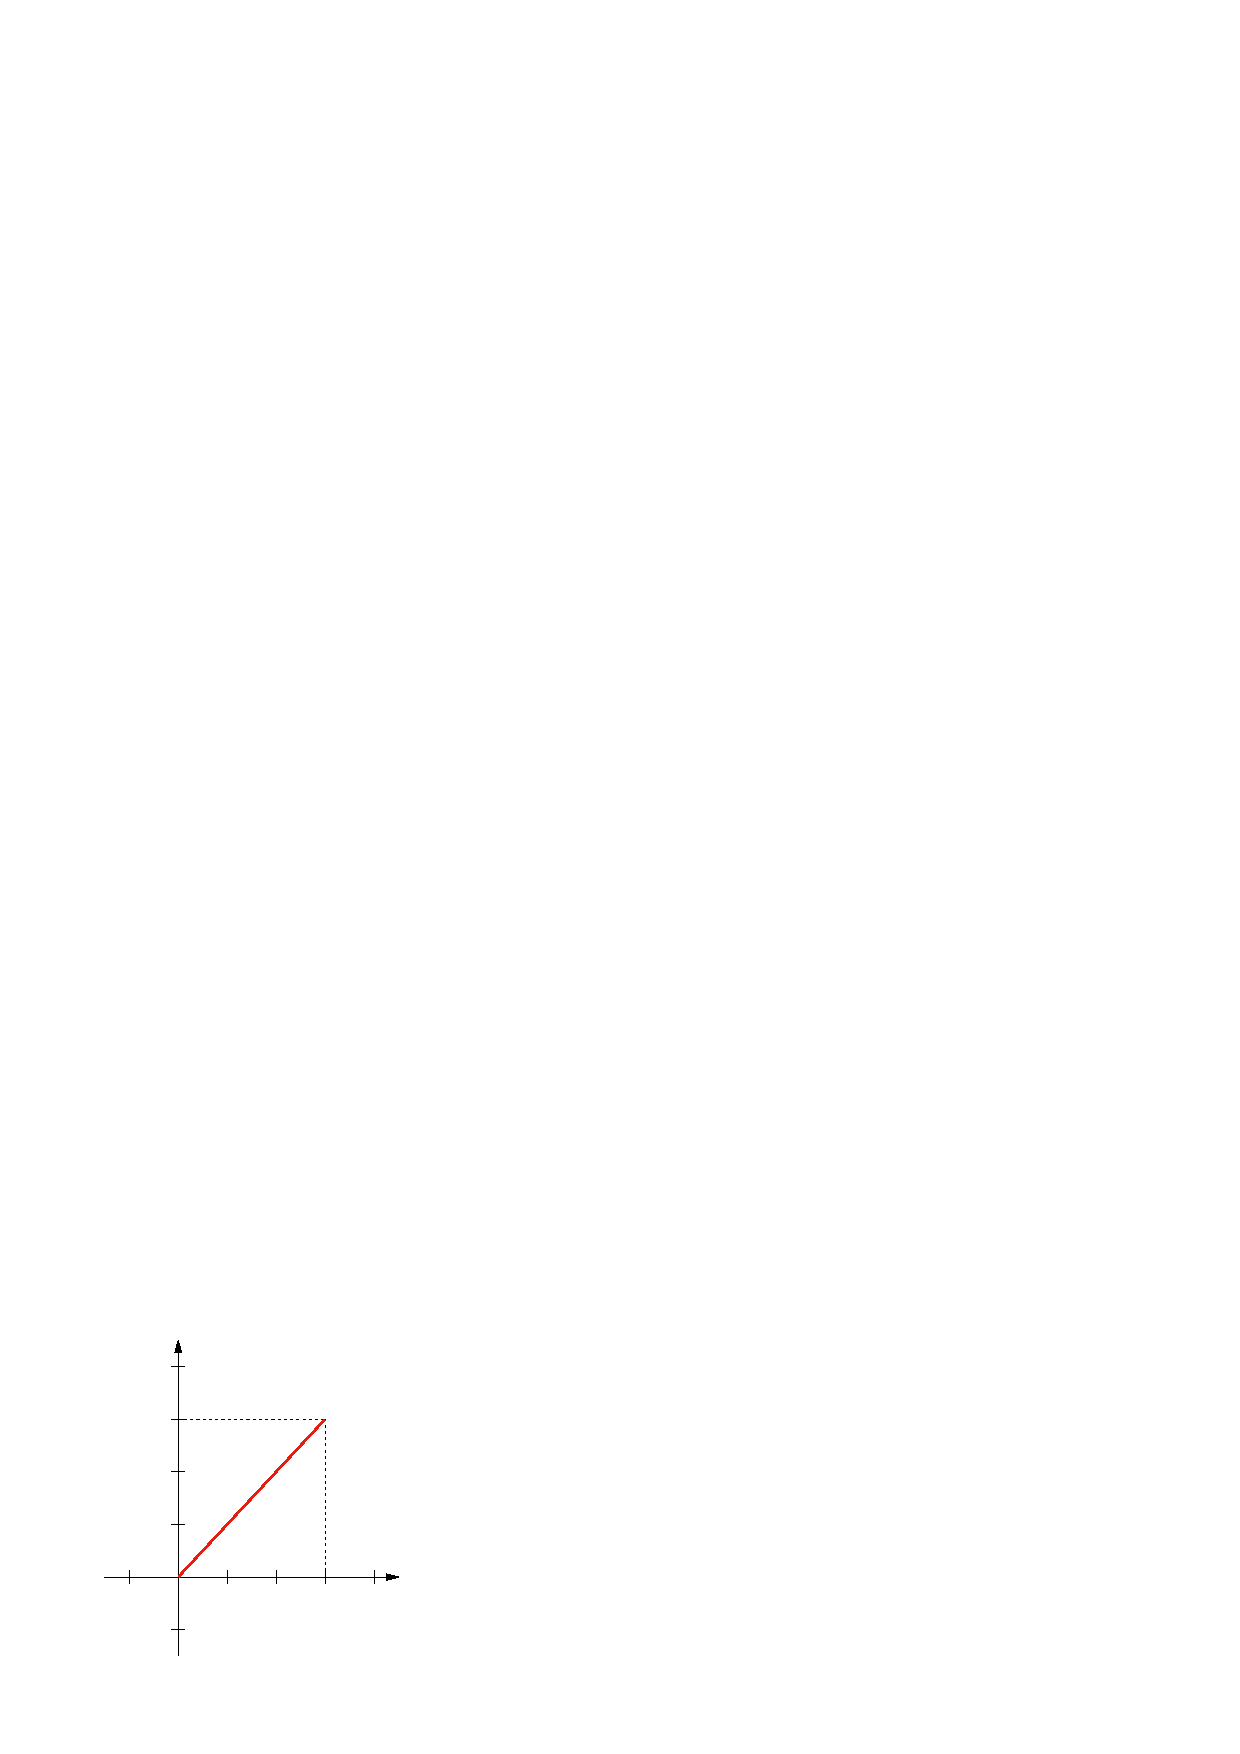
\includegraphics[width={144.00bp},height={144.00bp}]{figura_03_01}}%
    \gplfronttext
  \end{picture}%
\endgroup

\end{figure}
\begin{center}
    Unidad imaginaria: $i=j=\sqrt{-1}$\\
    Forma rectangular: $z=a+jb$\\
    Módulo: $|z|=\sqrt{a^2+b^2}$\\
    Argumento: $\theta=\arctan(\frac{b}{a})$\\
\end{center}

Forma polar:
\begin{equation*}
    z=|z|\cos(\theta)+j|z|\sen(\theta)
        =|z|(\cos(\theta)+j\sen(\theta))
\end{equation*}

Formula de \emph{Euler}:
\begin{equation}
    e^{j\theta}=\cos(\theta)+j\sen(\theta)
\end{equation}

Por tanto:
\begin{equation*}
    z=|z|e^{j\theta}
\end{equation*}

Forma exponencial o fasorial:
\begin{equation*}
    z=|z|\angle\theta
\end{equation*}

\subsection{Formas complejas del seno y coseno}
\begin{equation}
    e^{j\theta}=\cos(\theta)+j\sen(\theta)
    \label{e1}
\end{equation}
\begin{equation}
    e^{-j\theta}=\cos(\theta)-j\sen(\theta)
    \label{e2}
\end{equation}

Sumando las ecuaciones~\ref{e1} y~\ref{e2}:
\begin{equation*}
    e^{j\theta}+e^{-j\theta}=2\cos(\theta)
\end{equation*}
\begin{equation}
    \cos(\theta)=\frac{e^{j\theta}+e^{-j\theta}}{2}
\end{equation}

Restando las ecuaciones~\ref{e1} y~\ref{e2}:
\begin{equation*}
    e^{j\theta}-e^{-j\theta}=2j\sen(\theta)
\end{equation*}
\begin{equation}
    \sen(\theta)=\frac{e^{j\theta}-e^{-j\theta}}{2j}
\end{equation}

\subsection{Conjugado}
\begin{figure}[H]
    \centering
    % GNUPLOT: LaTeX picture with Postscript
\begingroup
  \makeatletter
  \providecommand\color[2][]{%
    \GenericError{(gnuplot) \space\space\space\@spaces}{%
      Package color not loaded in conjunction with
      terminal option `colourtext'%
    }{See the gnuplot documentation for explanation.%
    }{Either use 'blacktext' in gnuplot or load the package
      color.sty in LaTeX.}%
    \renewcommand\color[2][]{}%
  }%
  \providecommand\includegraphics[2][]{%
    \GenericError{(gnuplot) \space\space\space\@spaces}{%
      Package graphicx or graphics not loaded%
    }{See the gnuplot documentation for explanation.%
    }{The gnuplot epslatex terminal needs graphicx.sty or graphics.sty.}%
    \renewcommand\includegraphics[2][]{}%
  }%
  \providecommand\rotatebox[2]{#2}%
  \@ifundefined{ifGPcolor}{%
    \newif\ifGPcolor
    \GPcolorfalse
  }{}%
  \@ifundefined{ifGPblacktext}{%
    \newif\ifGPblacktext
    \GPblacktexttrue
  }{}%
  % define a \g@addto@macro without @ in the name:
  \let\gplgaddtomacro\g@addto@macro
  % define empty templates for all commands taking text:
  \gdef\gplbacktext{}%
  \gdef\gplfronttext{}%
  \makeatother
  \ifGPblacktext
    % no textcolor at all
    \def\colorrgb#1{}%
    \def\colorgray#1{}%
  \else
    % gray or color?
    \ifGPcolor
      \def\colorrgb#1{\color[rgb]{#1}}%
      \def\colorgray#1{\color[gray]{#1}}%
      \expandafter\def\csname LTw\endcsname{\color{white}}%
      \expandafter\def\csname LTb\endcsname{\color{black}}%
      \expandafter\def\csname LTa\endcsname{\color{black}}%
      \expandafter\def\csname LT0\endcsname{\color[rgb]{1,0,0}}%
      \expandafter\def\csname LT1\endcsname{\color[rgb]{0,1,0}}%
      \expandafter\def\csname LT2\endcsname{\color[rgb]{0,0,1}}%
      \expandafter\def\csname LT3\endcsname{\color[rgb]{1,0,1}}%
      \expandafter\def\csname LT4\endcsname{\color[rgb]{0,1,1}}%
      \expandafter\def\csname LT5\endcsname{\color[rgb]{1,1,0}}%
      \expandafter\def\csname LT6\endcsname{\color[rgb]{0,0,0}}%
      \expandafter\def\csname LT7\endcsname{\color[rgb]{1,0.3,0}}%
      \expandafter\def\csname LT8\endcsname{\color[rgb]{0.5,0.5,0.5}}%
    \else
      % gray
      \def\colorrgb#1{\color{black}}%
      \def\colorgray#1{\color[gray]{#1}}%
      \expandafter\def\csname LTw\endcsname{\color{white}}%
      \expandafter\def\csname LTb\endcsname{\color{black}}%
      \expandafter\def\csname LTa\endcsname{\color{black}}%
      \expandafter\def\csname LT0\endcsname{\color{black}}%
      \expandafter\def\csname LT1\endcsname{\color{black}}%
      \expandafter\def\csname LT2\endcsname{\color{black}}%
      \expandafter\def\csname LT3\endcsname{\color{black}}%
      \expandafter\def\csname LT4\endcsname{\color{black}}%
      \expandafter\def\csname LT5\endcsname{\color{black}}%
      \expandafter\def\csname LT6\endcsname{\color{black}}%
      \expandafter\def\csname LT7\endcsname{\color{black}}%
      \expandafter\def\csname LT8\endcsname{\color{black}}%
    \fi
  \fi
    \setlength{\unitlength}{0.0500bp}%
    \ifx\gptboxheight\undefined%
      \newlength{\gptboxheight}%
      \newlength{\gptboxwidth}%
      \newsavebox{\gptboxtext}%
    \fi%
    \setlength{\fboxrule}{0.5pt}%
    \setlength{\fboxsep}{1pt}%
    \definecolor{tbcol}{rgb}{1,1,1}%
\begin{picture}(3600.00,3600.00)%
    \gplgaddtomacro\gplbacktext{%
      \csname LTb\endcsname%%
      \put(1680,192){\makebox(0,0)[r]{\strut{}}}%
      \put(1680,598){\makebox(0,0)[r]{\strut{}}}%
      \put(1680,1004){\makebox(0,0)[r]{\strut{}}}%
      \put(1680,1410){\makebox(0,0)[r]{\strut{}}}%
      \put(1680,1816){\makebox(0,0)[r]{\strut{}}}%
      \put(1680,2221){\makebox(0,0)[r]{\strut{}}}%
      \put(1680,2627){\makebox(0,0)[r]{\strut{}}}%
      \put(1680,3033){\makebox(0,0)[r]{\strut{}}}%
      \put(1680,3439){\makebox(0,0)[r]{\strut{}}}%
      \put(240,1593){\makebox(0,0){\strut{}}}%
      \put(624,1593){\makebox(0,0){\strut{}}}%
      \put(1008,1593){\makebox(0,0){\strut{}}}%
      \put(1392,1593){\makebox(0,0){\strut{}}}%
      \put(1776,1593){\makebox(0,0){\strut{}}}%
      \put(2159,1593){\makebox(0,0){\strut{}}}%
      \put(2543,1593){\makebox(0,0){\strut{}}}%
      \put(2927,1593){\makebox(0,0){\strut{}}}%
      \put(3311,1593){\makebox(0,0){\strut{}}}%
      \csname LTb\endcsname%%
      \put(3695,1816){\makebox(0,0)[l]{\strut{}$\mathbb{R}e$}}%
      \put(1910,3540){\makebox(0,0)[l]{\strut{}$\mathbb{I}m$}}%
      \put(2927,3216){\makebox(0,0)[l]{\strut{}$z$}}%
      \put(2927,415){\makebox(0,0)[l]{\strut{}$z*$}}%
      \put(2889,1673){\makebox(0,0)[l]{\strut{}$a$}}%
      \put(1488,3053){\makebox(0,0)[l]{\strut{}$jb$}}%
      \put(1392,578){\makebox(0,0)[l]{\strut{}$-jb$}}%
      \put(2236,1978){\makebox(0,0)[l]{\strut{}$\theta$}}%
      \put(2236,1572){\makebox(0,0)[l]{\strut{}$-\theta$}}%
    }%
    \gplgaddtomacro\gplfronttext{%
    }%
    \gplgaddtomacro\gplbacktext{%
      \csname LTb\endcsname%%
      \put(1680,192){\makebox(0,0)[r]{\strut{}}}%
      \put(1680,598){\makebox(0,0)[r]{\strut{}}}%
      \put(1680,1004){\makebox(0,0)[r]{\strut{}}}%
      \put(1680,1410){\makebox(0,0)[r]{\strut{}}}%
      \put(1680,1816){\makebox(0,0)[r]{\strut{}}}%
      \put(1680,2221){\makebox(0,0)[r]{\strut{}}}%
      \put(1680,2627){\makebox(0,0)[r]{\strut{}}}%
      \put(1680,3033){\makebox(0,0)[r]{\strut{}}}%
      \put(1680,3439){\makebox(0,0)[r]{\strut{}}}%
      \put(240,1593){\makebox(0,0){\strut{}}}%
      \put(624,1593){\makebox(0,0){\strut{}}}%
      \put(1008,1593){\makebox(0,0){\strut{}}}%
      \put(1392,1593){\makebox(0,0){\strut{}}}%
      \put(1776,1593){\makebox(0,0){\strut{}}}%
      \put(2159,1593){\makebox(0,0){\strut{}}}%
      \put(2543,1593){\makebox(0,0){\strut{}}}%
      \put(2927,1593){\makebox(0,0){\strut{}}}%
      \put(3311,1593){\makebox(0,0){\strut{}}}%
      \csname LTb\endcsname%%
      \put(3695,1816){\makebox(0,0)[l]{\strut{}$\mathbb{R}e$}}%
      \put(1910,3540){\makebox(0,0)[l]{\strut{}$\mathbb{I}m$}}%
      \put(2927,3216){\makebox(0,0)[l]{\strut{}$z$}}%
      \put(2927,415){\makebox(0,0)[l]{\strut{}$z*$}}%
      \put(2889,1673){\makebox(0,0)[l]{\strut{}$a$}}%
      \put(1488,3053){\makebox(0,0)[l]{\strut{}$jb$}}%
      \put(1392,578){\makebox(0,0)[l]{\strut{}$-jb$}}%
      \put(2236,1978){\makebox(0,0)[l]{\strut{}$\theta$}}%
      \put(2236,1572){\makebox(0,0)[l]{\strut{}$-\theta$}}%
    }%
    \gplgaddtomacro\gplfronttext{%
    }%
    \gplgaddtomacro\gplbacktext{%
      \csname LTb\endcsname%%
      \put(1680,192){\makebox(0,0)[r]{\strut{}}}%
      \put(1680,598){\makebox(0,0)[r]{\strut{}}}%
      \put(1680,1004){\makebox(0,0)[r]{\strut{}}}%
      \put(1680,1410){\makebox(0,0)[r]{\strut{}}}%
      \put(1680,1816){\makebox(0,0)[r]{\strut{}}}%
      \put(1680,2221){\makebox(0,0)[r]{\strut{}}}%
      \put(1680,2627){\makebox(0,0)[r]{\strut{}}}%
      \put(1680,3033){\makebox(0,0)[r]{\strut{}}}%
      \put(1680,3439){\makebox(0,0)[r]{\strut{}}}%
      \put(240,1593){\makebox(0,0){\strut{}}}%
      \put(624,1593){\makebox(0,0){\strut{}}}%
      \put(1008,1593){\makebox(0,0){\strut{}}}%
      \put(1392,1593){\makebox(0,0){\strut{}}}%
      \put(1776,1593){\makebox(0,0){\strut{}}}%
      \put(2159,1593){\makebox(0,0){\strut{}}}%
      \put(2543,1593){\makebox(0,0){\strut{}}}%
      \put(2927,1593){\makebox(0,0){\strut{}}}%
      \put(3311,1593){\makebox(0,0){\strut{}}}%
      \csname LTb\endcsname%%
      \put(3695,1816){\makebox(0,0)[l]{\strut{}$\mathbb{R}e$}}%
      \put(1910,3540){\makebox(0,0)[l]{\strut{}$\mathbb{I}m$}}%
      \put(2927,3216){\makebox(0,0)[l]{\strut{}$z$}}%
      \put(2927,415){\makebox(0,0)[l]{\strut{}$z*$}}%
      \put(2889,1673){\makebox(0,0)[l]{\strut{}$a$}}%
      \put(1488,3053){\makebox(0,0)[l]{\strut{}$jb$}}%
      \put(1392,578){\makebox(0,0)[l]{\strut{}$-jb$}}%
      \put(2236,1978){\makebox(0,0)[l]{\strut{}$\theta$}}%
      \put(2236,1572){\makebox(0,0)[l]{\strut{}$-\theta$}}%
    }%
    \gplgaddtomacro\gplfronttext{%
    }%
    \gplgaddtomacro\gplbacktext{%
      \csname LTb\endcsname%%
      \put(1680,192){\makebox(0,0)[r]{\strut{}}}%
      \put(1680,598){\makebox(0,0)[r]{\strut{}}}%
      \put(1680,1004){\makebox(0,0)[r]{\strut{}}}%
      \put(1680,1410){\makebox(0,0)[r]{\strut{}}}%
      \put(1680,1816){\makebox(0,0)[r]{\strut{}}}%
      \put(1680,2221){\makebox(0,0)[r]{\strut{}}}%
      \put(1680,2627){\makebox(0,0)[r]{\strut{}}}%
      \put(1680,3033){\makebox(0,0)[r]{\strut{}}}%
      \put(1680,3439){\makebox(0,0)[r]{\strut{}}}%
      \put(240,1593){\makebox(0,0){\strut{}}}%
      \put(624,1593){\makebox(0,0){\strut{}}}%
      \put(1008,1593){\makebox(0,0){\strut{}}}%
      \put(1392,1593){\makebox(0,0){\strut{}}}%
      \put(1776,1593){\makebox(0,0){\strut{}}}%
      \put(2159,1593){\makebox(0,0){\strut{}}}%
      \put(2543,1593){\makebox(0,0){\strut{}}}%
      \put(2927,1593){\makebox(0,0){\strut{}}}%
      \put(3311,1593){\makebox(0,0){\strut{}}}%
      \csname LTb\endcsname%%
      \put(3695,1816){\makebox(0,0)[l]{\strut{}$\mathbb{R}e$}}%
      \put(1910,3540){\makebox(0,0)[l]{\strut{}$\mathbb{I}m$}}%
      \put(2927,3216){\makebox(0,0)[l]{\strut{}$z$}}%
      \put(2927,415){\makebox(0,0)[l]{\strut{}$z*$}}%
      \put(2889,1673){\makebox(0,0)[l]{\strut{}$a$}}%
      \put(1488,3053){\makebox(0,0)[l]{\strut{}$jb$}}%
      \put(1392,578){\makebox(0,0)[l]{\strut{}$-jb$}}%
      \put(2236,1978){\makebox(0,0)[l]{\strut{}$\theta$}}%
      \put(2236,1572){\makebox(0,0)[l]{\strut{}$-\theta$}}%
    }%
    \gplgaddtomacro\gplfronttext{%
    }%
    \gplbacktext
    \put(0,0){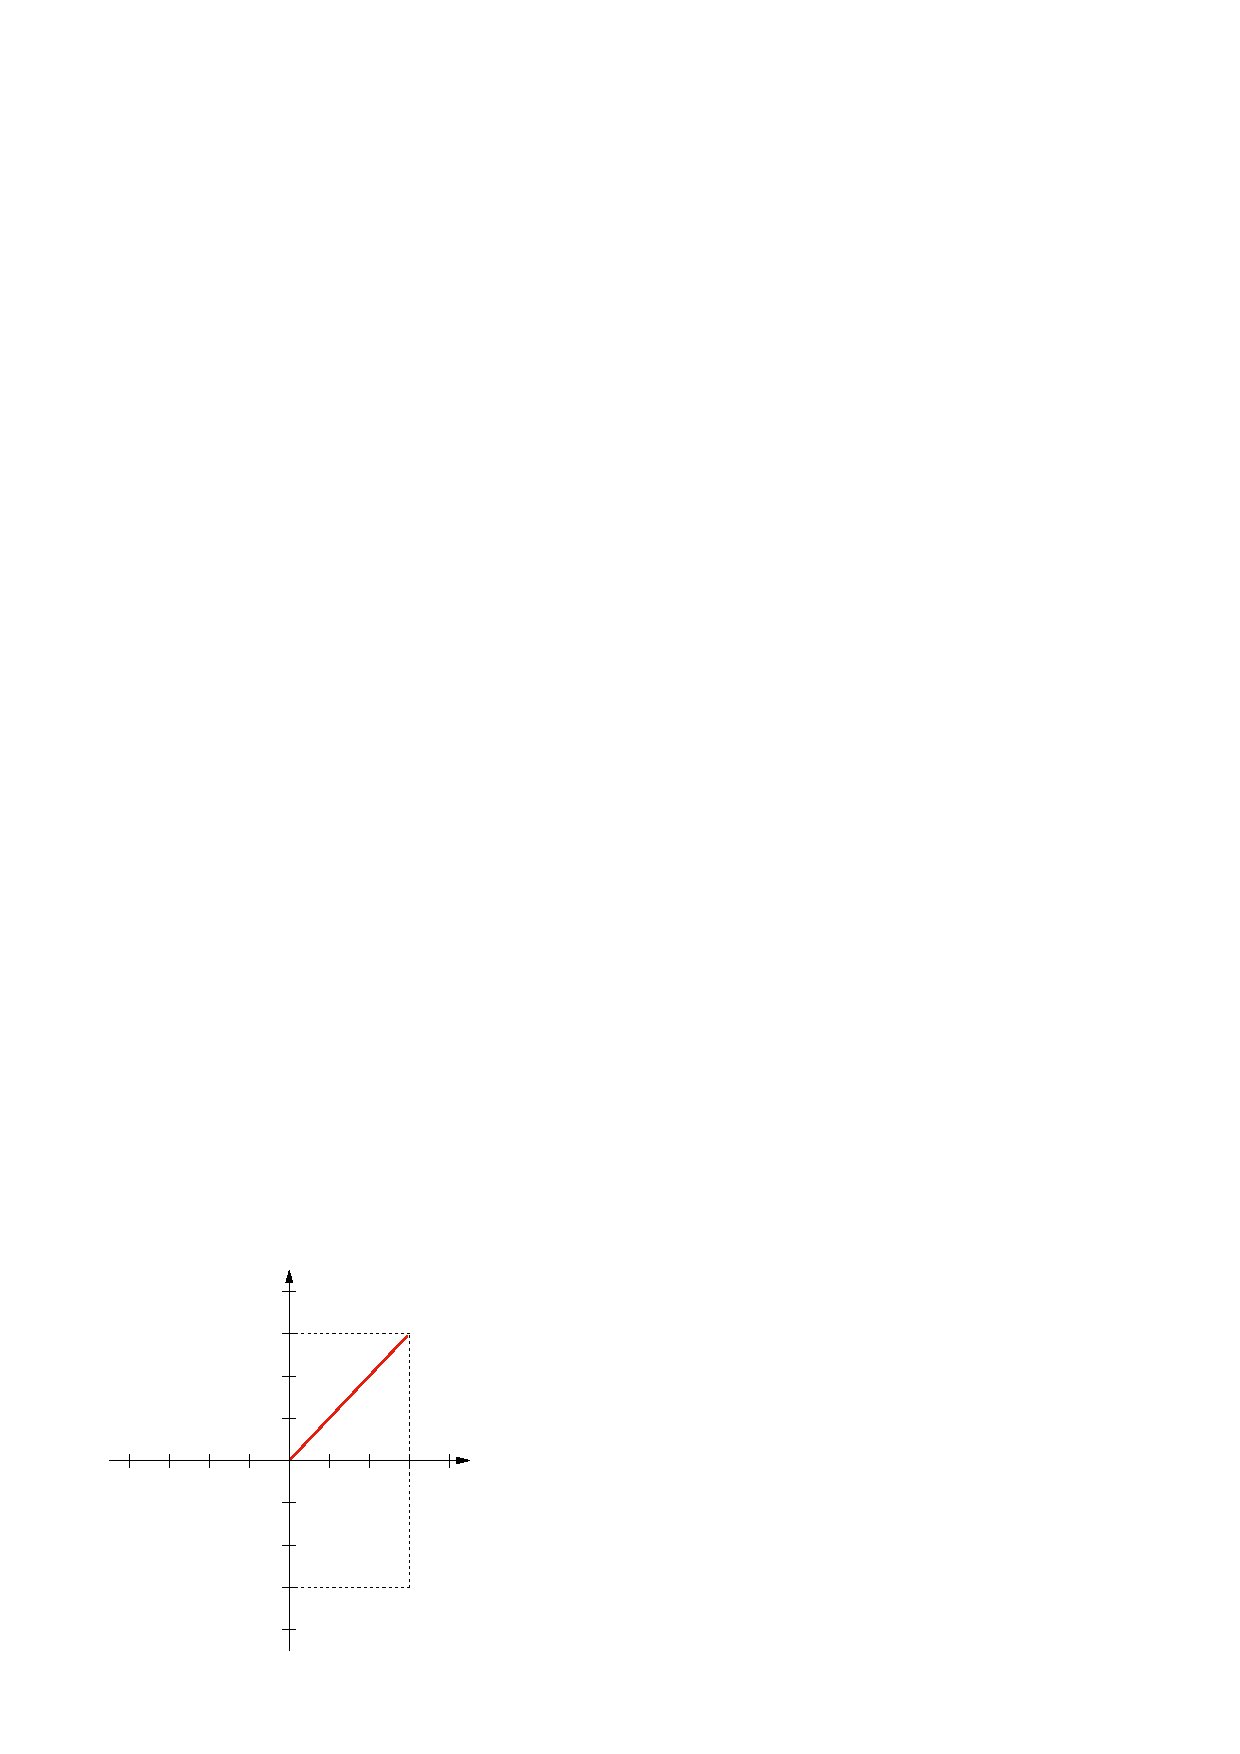
\includegraphics[width={180.00bp},height={180.00bp}]{figura_03_02}}%
    \gplfronttext
  \end{picture}%
\endgroup

\end{figure}
\begin{equation*}
    z=a+jb=|z|\angle\theta
\end{equation*}
\begin{equation*}
    z*=a-jb=|z|\angle-\theta
\end{equation*}
\begin{equation*}
    (z)(z*)={|z|}^2
\end{equation*}

\section{Serie compleja de \emph{Fourier}}
Partiendo de la serie trigonométrica de \emph{Fourier}:
\begin{equation*}
    f(t)=\frac{a_0}{2}+
    \sum_{n=1}^{\infty}\left[
        a_n\cos(n\omega_0\,t)+
        b_n\sen(n\omega_0\,t)
    \right]
\end{equation*}
\begin{equation*}
    f(t)=\frac{a_0}{2}+
    \sum_{n=1}^{\infty}\left[
        a_n\left(
            \frac{e^{jn\omega_0\,t}+e^{-jn\omega_0\,t}
            }{2}
        \right)+
        b_n\left(
            \frac{e^{jn\omega_0\,t}+e^{-jn\omega_0\,t}
            }{2j}
        \right)
    \right]
\end{equation*}
\begin{equation*}
    \frac{1}{j}=-j
\end{equation*}
\begin{equation*}
    f(t)=\frac{a_0}{2}+
    \sum_{n=1}^{\infty}\left[
        a_n\left(
            \frac{e^{jn\omega_0\,t}+e^{-jn\omega_0\,t}
            }{2}
        \right)-
        jb_n\left(
            \frac{e^{jn\omega_0\,t}+e^{-jn\omega_0\,t}
            }{2}
        \right)
    \right]
\end{equation*}
\begin{equation*}
    f(t)=\frac{a_0}{2}+
    \sum_{n=1}^{\infty}\left[
        \left(\frac{a_n-jb_n}{2}\right)e^{jn\omega_0\,t}+
        \left(\frac{a_n+jb_n}{2}\right)e^{-jn\omega_0\,t}
    \right]
\end{equation*}
\begin{equation*}
    f(t)=\frac{a_0}{2}+
    \sum_{n=1}^{\infty}\left[
        \left(\frac{a_n-jb_n}{2}\right)e^{jn\omega_0\,t}
    \right]+
    \sum_{n=1}^{\infty}\left[
        \left(\frac{a_n+jb_n}{2}\right)e^{-jn\omega_0\,t}
    \right]
\end{equation*}
\begin{equation*}
    f(t)=\frac{a_0}{2}+
    \sum_{n=1}^{\infty}\left[
        \left(\frac{a_n-jb_n}{2}\right)e^{jn\omega_0\,t}
    \right]+
    \sum_{-n=1}^{\infty}\left[
        \left(\frac{a_{-n}+jb_{-n}}{2}\right)e^{jn\omega_0\,t}
    \right]
\end{equation*}
\begin{equation*}
    f(t)=\frac{a_0}{2}+
    \sum_{n=1}^{\infty}\left[
        \left(\frac{a_n-jb_n}{2}\right)e^{jn\omega_0\,t}
    \right]+
    \sum_{n=-1}^{-\infty}\left[
        \left(\frac{a_n+jb_n}{2}\right)e^{jn\omega_0\,t}
    \right]
\end{equation*}
\begin{equation*}
    f(t)=\frac{a_0}{2}+
    \sum_{\substack{n=-\infty\\n\neq0}}^{\infty}
        \left(\frac{a_n-jb_n}{2}\right)e^{jn\omega_0\,t}
\end{equation*}

Sean los coeficientes complejos de \emph{Fourier}:
\begin{equation*}
    c_n=\frac{a_n-jb_n}{2}
\end{equation*}
\begin{equation*}
    c_0=\frac{a_0}{2}
\end{equation*}

Entonces:
\begin{equation*}
    f(t)=c_0+\sum_{\substack{n=-\infty\\n\neq0}}^{\infty}c_n\,e^{jn\omega_0\,t}
\end{equation*}
\begin{equation}
    f(t)=\sum_{n=-\infty}^{\infty}c_n\,e^{jn\omega_0\,t}
\end{equation}

\subsection{Evaluación del coeficiente complejo de \emph{Fourier}}
\begin{equation*}
\begin{split}
    c_n
        &=\frac{a_n-jb_n}{2}\\
        &=\frac{1}{2}\left[
            \frac{2}{T}\int_0^T\,f(t)\cos(n\omega_0\,t)\,dt
            -j\frac{2}{T}\int_0^T\,f(t)\sen(n\omega_0\,t)\,dt
        \right]\\
        &=\frac{1}{T}\int_0^T\,f(t)\left[
            \cos(n\omega_0\,t)-j\sen(n\omega_0\,t)
        \right]dt\\
        &=\frac{1}{T}\int_0^T\,f(t)\,e^{-jn\omega_0\,t}\,dt\\
\end{split}
\end{equation*}
\begin{equation}
    c_n=\frac{1}{T}\int_0^T\,f(t)\,e^{-jn\omega_0\,t}\,dt
\end{equation}

En particular:
\begin{equation}
    c_0=\frac{1}{T}\int_0^T\,f(t)\,dt
\end{equation}

\subsection{Relación entre el coeficiente complejo y los coeficientes
trigonométricos}
\begin{equation*}
    c_n=\frac{a_n-jbn}{2}
        =\frac{a_n}{2}+j\frac{-b_n}{2}
\end{equation*}
\begin{equation*}
    \frac{a_n}{2}=\mathbb{R}e\{c_n\}
\end{equation*}
\begin{equation}
    a_n=2\,\mathbb{R}e\{c_n\}
\end{equation}
\begin{equation*}
    -\frac{b_n}{2}=\mathbb{I}m\{c_n\}
\end{equation*}
\begin{equation}
    b_n=-2\,\mathbb{I}m\{c_n\}
\end{equation}

\section{Ondas senoidales rectificadas}
\subsection{Rectificación de media onda}
\begin{equation*}
    f(t)=\begin{cases}
        A\sen(\omega_0\,t)&0<t<T/2\\
        0&T/2<t<T\\
    \end{cases}
\end{equation*}
\begin{equation*}
    T=\frac{2\pi}{\omega_0}
\end{equation*}
\begin{figure}[H]
    \centering
    % GNUPLOT: LaTeX picture with Postscript
\begingroup
  \makeatletter
  \providecommand\color[2][]{%
    \GenericError{(gnuplot) \space\space\space\@spaces}{%
      Package color not loaded in conjunction with
      terminal option `colourtext'%
    }{See the gnuplot documentation for explanation.%
    }{Either use 'blacktext' in gnuplot or load the package
      color.sty in LaTeX.}%
    \renewcommand\color[2][]{}%
  }%
  \providecommand\includegraphics[2][]{%
    \GenericError{(gnuplot) \space\space\space\@spaces}{%
      Package graphicx or graphics not loaded%
    }{See the gnuplot documentation for explanation.%
    }{The gnuplot epslatex terminal needs graphicx.sty or graphics.sty.}%
    \renewcommand\includegraphics[2][]{}%
  }%
  \providecommand\rotatebox[2]{#2}%
  \@ifundefined{ifGPcolor}{%
    \newif\ifGPcolor
    \GPcolorfalse
  }{}%
  \@ifundefined{ifGPblacktext}{%
    \newif\ifGPblacktext
    \GPblacktexttrue
  }{}%
  % define a \g@addto@macro without @ in the name:
  \let\gplgaddtomacro\g@addto@macro
  % define empty templates for all commands taking text:
  \gdef\gplbacktext{}%
  \gdef\gplfronttext{}%
  \makeatother
  \ifGPblacktext
    % no textcolor at all
    \def\colorrgb#1{}%
    \def\colorgray#1{}%
  \else
    % gray or color?
    \ifGPcolor
      \def\colorrgb#1{\color[rgb]{#1}}%
      \def\colorgray#1{\color[gray]{#1}}%
      \expandafter\def\csname LTw\endcsname{\color{white}}%
      \expandafter\def\csname LTb\endcsname{\color{black}}%
      \expandafter\def\csname LTa\endcsname{\color{black}}%
      \expandafter\def\csname LT0\endcsname{\color[rgb]{1,0,0}}%
      \expandafter\def\csname LT1\endcsname{\color[rgb]{0,1,0}}%
      \expandafter\def\csname LT2\endcsname{\color[rgb]{0,0,1}}%
      \expandafter\def\csname LT3\endcsname{\color[rgb]{1,0,1}}%
      \expandafter\def\csname LT4\endcsname{\color[rgb]{0,1,1}}%
      \expandafter\def\csname LT5\endcsname{\color[rgb]{1,1,0}}%
      \expandafter\def\csname LT6\endcsname{\color[rgb]{0,0,0}}%
      \expandafter\def\csname LT7\endcsname{\color[rgb]{1,0.3,0}}%
      \expandafter\def\csname LT8\endcsname{\color[rgb]{0.5,0.5,0.5}}%
    \else
      % gray
      \def\colorrgb#1{\color{black}}%
      \def\colorgray#1{\color[gray]{#1}}%
      \expandafter\def\csname LTw\endcsname{\color{white}}%
      \expandafter\def\csname LTb\endcsname{\color{black}}%
      \expandafter\def\csname LTa\endcsname{\color{black}}%
      \expandafter\def\csname LT0\endcsname{\color{black}}%
      \expandafter\def\csname LT1\endcsname{\color{black}}%
      \expandafter\def\csname LT2\endcsname{\color{black}}%
      \expandafter\def\csname LT3\endcsname{\color{black}}%
      \expandafter\def\csname LT4\endcsname{\color{black}}%
      \expandafter\def\csname LT5\endcsname{\color{black}}%
      \expandafter\def\csname LT6\endcsname{\color{black}}%
      \expandafter\def\csname LT7\endcsname{\color{black}}%
      \expandafter\def\csname LT8\endcsname{\color{black}}%
    \fi
  \fi
    \setlength{\unitlength}{0.0500bp}%
    \ifx\gptboxheight\undefined%
      \newlength{\gptboxheight}%
      \newlength{\gptboxwidth}%
      \newsavebox{\gptboxtext}%
    \fi%
    \setlength{\fboxrule}{0.5pt}%
    \setlength{\fboxsep}{1pt}%
    \definecolor{tbcol}{rgb}{1,1,1}%
\begin{picture}(5472.00,2014.00)%
    \gplgaddtomacro\gplbacktext{%
      \csname LTb\endcsname%%
      \put(1909,469){\makebox(0,0)[r]{\strut{}}}%
      \put(1909,1023){\makebox(0,0)[r]{\strut{}}}%
      \put(1909,1576){\makebox(0,0)[r]{\strut{}}}%
      \put(593,800){\makebox(0,0){\strut{}}}%
      \put(1299,800){\makebox(0,0){\strut{}}}%
      \put(2005,800){\makebox(0,0){\strut{}}}%
      \put(2712,800){\makebox(0,0){\strut{}}}%
      \put(3418,800){\makebox(0,0){\strut{}}}%
      \put(4124,800){\makebox(0,0){\strut{}}}%
      \put(4830,800){\makebox(0,0){\strut{}}}%
      \csname LTb\endcsname%%
      \put(5360,1023){\makebox(0,0)[l]{\strut{}$t$}}%
      \put(2005,1991){\makebox(0,0)[l]{\strut{}$f(t)$}}%
      \put(2655,137){\makebox(0,0)[l]{\strut{}$T$}}%
    }%
    \gplgaddtomacro\gplfronttext{%
    }%
    \gplgaddtomacro\gplbacktext{%
      \csname LTb\endcsname%%
      \put(1909,469){\makebox(0,0)[r]{\strut{}}}%
      \put(1909,1023){\makebox(0,0)[r]{\strut{}}}%
      \put(1909,1576){\makebox(0,0)[r]{\strut{}}}%
      \put(593,800){\makebox(0,0){\strut{}}}%
      \put(1299,800){\makebox(0,0){\strut{}}}%
      \put(2005,800){\makebox(0,0){\strut{}}}%
      \put(2712,800){\makebox(0,0){\strut{}}}%
      \put(3418,800){\makebox(0,0){\strut{}}}%
      \put(4124,800){\makebox(0,0){\strut{}}}%
      \put(4830,800){\makebox(0,0){\strut{}}}%
      \csname LTb\endcsname%%
      \put(5360,1023){\makebox(0,0)[l]{\strut{}$t$}}%
      \put(2005,1991){\makebox(0,0)[l]{\strut{}$f(t)$}}%
      \put(2655,137){\makebox(0,0)[l]{\strut{}$T$}}%
    }%
    \gplgaddtomacro\gplfronttext{%
    }%
    \gplgaddtomacro\gplbacktext{%
      \csname LTb\endcsname%%
      \put(1909,469){\makebox(0,0)[r]{\strut{}}}%
      \put(1909,1023){\makebox(0,0)[r]{\strut{}}}%
      \put(1909,1576){\makebox(0,0)[r]{\strut{}}}%
      \put(593,800){\makebox(0,0){\strut{}}}%
      \put(1299,800){\makebox(0,0){\strut{}}}%
      \put(2005,800){\makebox(0,0){\strut{}}}%
      \put(2712,800){\makebox(0,0){\strut{}}}%
      \put(3418,800){\makebox(0,0){\strut{}}}%
      \put(4124,800){\makebox(0,0){\strut{}}}%
      \put(4830,800){\makebox(0,0){\strut{}}}%
      \csname LTb\endcsname%%
      \put(5360,1023){\makebox(0,0)[l]{\strut{}$t$}}%
      \put(2005,1991){\makebox(0,0)[l]{\strut{}$f(t)$}}%
      \put(2655,137){\makebox(0,0)[l]{\strut{}$T$}}%
    }%
    \gplgaddtomacro\gplfronttext{%
    }%
    \gplgaddtomacro\gplbacktext{%
      \csname LTb\endcsname%%
      \put(1909,469){\makebox(0,0)[r]{\strut{}}}%
      \put(1909,1023){\makebox(0,0)[r]{\strut{}}}%
      \put(1909,1576){\makebox(0,0)[r]{\strut{}}}%
      \put(593,800){\makebox(0,0){\strut{}}}%
      \put(1299,800){\makebox(0,0){\strut{}}}%
      \put(2005,800){\makebox(0,0){\strut{}}}%
      \put(2712,800){\makebox(0,0){\strut{}}}%
      \put(3418,800){\makebox(0,0){\strut{}}}%
      \put(4124,800){\makebox(0,0){\strut{}}}%
      \put(4830,800){\makebox(0,0){\strut{}}}%
      \csname LTb\endcsname%%
      \put(5360,1023){\makebox(0,0)[l]{\strut{}$t$}}%
      \put(2005,1991){\makebox(0,0)[l]{\strut{}$f(t)$}}%
      \put(2655,137){\makebox(0,0)[l]{\strut{}$T$}}%
    }%
    \gplgaddtomacro\gplfronttext{%
    }%
    \gplgaddtomacro\gplbacktext{%
      \csname LTb\endcsname%%
      \put(1909,469){\makebox(0,0)[r]{\strut{}}}%
      \put(1909,1023){\makebox(0,0)[r]{\strut{}}}%
      \put(1909,1576){\makebox(0,0)[r]{\strut{}}}%
      \put(593,800){\makebox(0,0){\strut{}}}%
      \put(1299,800){\makebox(0,0){\strut{}}}%
      \put(2005,800){\makebox(0,0){\strut{}}}%
      \put(2712,800){\makebox(0,0){\strut{}}}%
      \put(3418,800){\makebox(0,0){\strut{}}}%
      \put(4124,800){\makebox(0,0){\strut{}}}%
      \put(4830,800){\makebox(0,0){\strut{}}}%
      \csname LTb\endcsname%%
      \put(5360,1023){\makebox(0,0)[l]{\strut{}$t$}}%
      \put(2005,1991){\makebox(0,0)[l]{\strut{}$f(t)$}}%
      \put(2655,137){\makebox(0,0)[l]{\strut{}$T$}}%
    }%
    \gplgaddtomacro\gplfronttext{%
    }%
    \gplgaddtomacro\gplbacktext{%
      \csname LTb\endcsname%%
      \put(1909,469){\makebox(0,0)[r]{\strut{}}}%
      \put(1909,1023){\makebox(0,0)[r]{\strut{}}}%
      \put(1909,1576){\makebox(0,0)[r]{\strut{}}}%
      \put(593,800){\makebox(0,0){\strut{}}}%
      \put(1299,800){\makebox(0,0){\strut{}}}%
      \put(2005,800){\makebox(0,0){\strut{}}}%
      \put(2712,800){\makebox(0,0){\strut{}}}%
      \put(3418,800){\makebox(0,0){\strut{}}}%
      \put(4124,800){\makebox(0,0){\strut{}}}%
      \put(4830,800){\makebox(0,0){\strut{}}}%
      \csname LTb\endcsname%%
      \put(5360,1023){\makebox(0,0)[l]{\strut{}$t$}}%
      \put(2005,1991){\makebox(0,0)[l]{\strut{}$f(t)$}}%
      \put(2655,137){\makebox(0,0)[l]{\strut{}$T$}}%
    }%
    \gplgaddtomacro\gplfronttext{%
    }%
    \gplbacktext
    \put(0,0){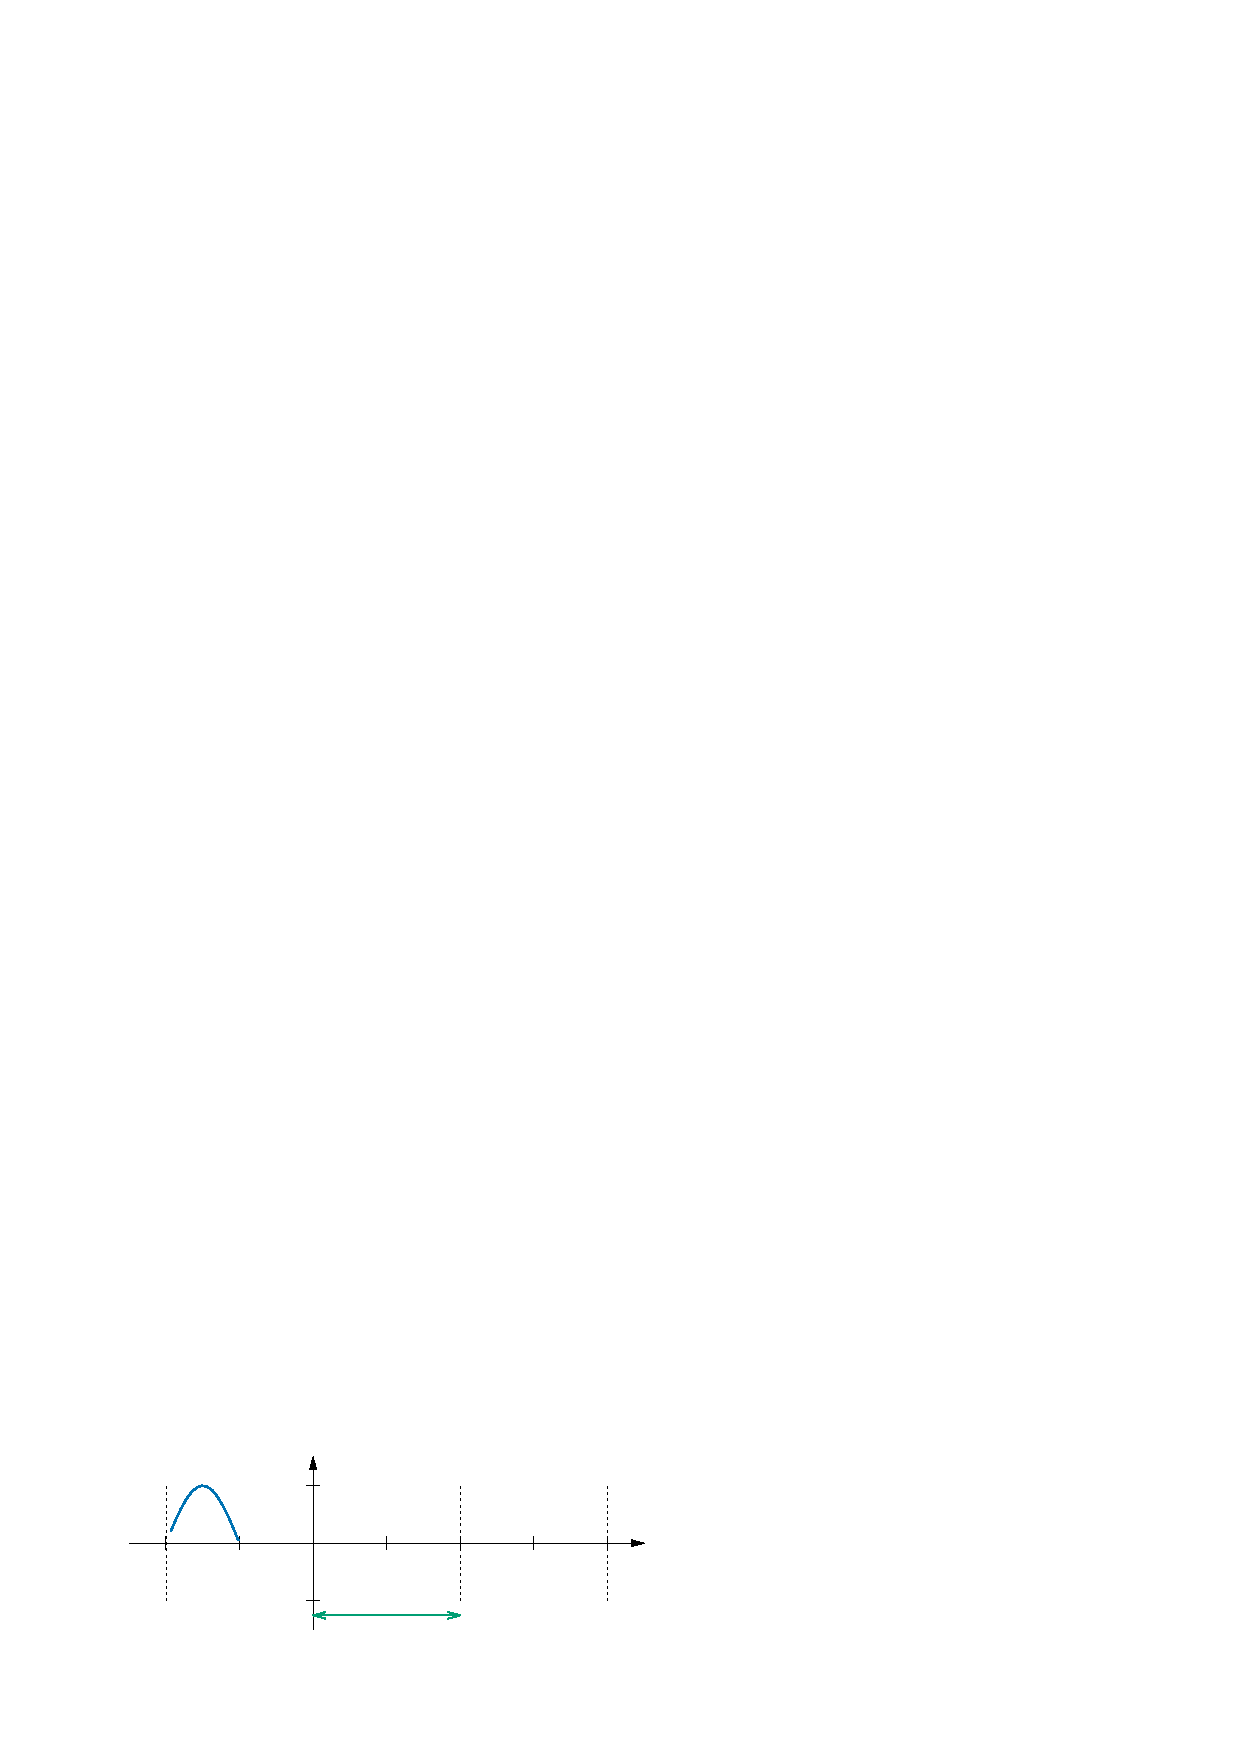
\includegraphics[width={273.60bp},height={100.70bp}]{figura_03_03}}%
    \gplfronttext
  \end{picture}%
\endgroup

\end{figure}

El periodo de la onda rectificada es el mismo que de la onda original.

\subsection{Rectificación de onda completa}
\begin{equation*}
    f(t)=A\,|\sen(\omega_0\,t)|
\end{equation*}
\begin{figure}[H]
    \centering
    % GNUPLOT: LaTeX picture with Postscript
\begingroup
  \makeatletter
  \providecommand\color[2][]{%
    \GenericError{(gnuplot) \space\space\space\@spaces}{%
      Package color not loaded in conjunction with
      terminal option `colourtext'%
    }{See the gnuplot documentation for explanation.%
    }{Either use 'blacktext' in gnuplot or load the package
      color.sty in LaTeX.}%
    \renewcommand\color[2][]{}%
  }%
  \providecommand\includegraphics[2][]{%
    \GenericError{(gnuplot) \space\space\space\@spaces}{%
      Package graphicx or graphics not loaded%
    }{See the gnuplot documentation for explanation.%
    }{The gnuplot epslatex terminal needs graphicx.sty or graphics.sty.}%
    \renewcommand\includegraphics[2][]{}%
  }%
  \providecommand\rotatebox[2]{#2}%
  \@ifundefined{ifGPcolor}{%
    \newif\ifGPcolor
    \GPcolorfalse
  }{}%
  \@ifundefined{ifGPblacktext}{%
    \newif\ifGPblacktext
    \GPblacktexttrue
  }{}%
  % define a \g@addto@macro without @ in the name:
  \let\gplgaddtomacro\g@addto@macro
  % define empty templates for all commands taking text:
  \gdef\gplbacktext{}%
  \gdef\gplfronttext{}%
  \makeatother
  \ifGPblacktext
    % no textcolor at all
    \def\colorrgb#1{}%
    \def\colorgray#1{}%
  \else
    % gray or color?
    \ifGPcolor
      \def\colorrgb#1{\color[rgb]{#1}}%
      \def\colorgray#1{\color[gray]{#1}}%
      \expandafter\def\csname LTw\endcsname{\color{white}}%
      \expandafter\def\csname LTb\endcsname{\color{black}}%
      \expandafter\def\csname LTa\endcsname{\color{black}}%
      \expandafter\def\csname LT0\endcsname{\color[rgb]{1,0,0}}%
      \expandafter\def\csname LT1\endcsname{\color[rgb]{0,1,0}}%
      \expandafter\def\csname LT2\endcsname{\color[rgb]{0,0,1}}%
      \expandafter\def\csname LT3\endcsname{\color[rgb]{1,0,1}}%
      \expandafter\def\csname LT4\endcsname{\color[rgb]{0,1,1}}%
      \expandafter\def\csname LT5\endcsname{\color[rgb]{1,1,0}}%
      \expandafter\def\csname LT6\endcsname{\color[rgb]{0,0,0}}%
      \expandafter\def\csname LT7\endcsname{\color[rgb]{1,0.3,0}}%
      \expandafter\def\csname LT8\endcsname{\color[rgb]{0.5,0.5,0.5}}%
    \else
      % gray
      \def\colorrgb#1{\color{black}}%
      \def\colorgray#1{\color[gray]{#1}}%
      \expandafter\def\csname LTw\endcsname{\color{white}}%
      \expandafter\def\csname LTb\endcsname{\color{black}}%
      \expandafter\def\csname LTa\endcsname{\color{black}}%
      \expandafter\def\csname LT0\endcsname{\color{black}}%
      \expandafter\def\csname LT1\endcsname{\color{black}}%
      \expandafter\def\csname LT2\endcsname{\color{black}}%
      \expandafter\def\csname LT3\endcsname{\color{black}}%
      \expandafter\def\csname LT4\endcsname{\color{black}}%
      \expandafter\def\csname LT5\endcsname{\color{black}}%
      \expandafter\def\csname LT6\endcsname{\color{black}}%
      \expandafter\def\csname LT7\endcsname{\color{black}}%
      \expandafter\def\csname LT8\endcsname{\color{black}}%
    \fi
  \fi
    \setlength{\unitlength}{0.0500bp}%
    \ifx\gptboxheight\undefined%
      \newlength{\gptboxheight}%
      \newlength{\gptboxwidth}%
      \newsavebox{\gptboxtext}%
    \fi%
    \setlength{\fboxrule}{0.5pt}%
    \setlength{\fboxsep}{1pt}%
    \definecolor{tbcol}{rgb}{1,1,1}%
\begin{picture}(5472.00,2014.00)%
    \gplgaddtomacro\gplbacktext{%
      \csname LTb\endcsname%%
      \put(1909,469){\makebox(0,0)[r]{\strut{}}}%
      \put(1909,1023){\makebox(0,0)[r]{\strut{}}}%
      \put(1909,1576){\makebox(0,0)[r]{\strut{}}}%
      \put(593,800){\makebox(0,0){\strut{}}}%
      \put(1299,800){\makebox(0,0){\strut{}}}%
      \put(2005,800){\makebox(0,0){\strut{}}}%
      \put(2712,800){\makebox(0,0){\strut{}}}%
      \put(3418,800){\makebox(0,0){\strut{}}}%
      \put(4124,800){\makebox(0,0){\strut{}}}%
      \put(4830,800){\makebox(0,0){\strut{}}}%
      \csname LTb\endcsname%%
      \put(5360,1023){\makebox(0,0)[l]{\strut{}$t$}}%
      \put(2005,1991){\makebox(0,0)[l]{\strut{}$f(t)$}}%
      \put(2330,137){\makebox(0,0)[l]{\strut{}$T$}}%
    }%
    \gplgaddtomacro\gplfronttext{%
    }%
    \gplgaddtomacro\gplbacktext{%
      \csname LTb\endcsname%%
      \put(1909,469){\makebox(0,0)[r]{\strut{}}}%
      \put(1909,1023){\makebox(0,0)[r]{\strut{}}}%
      \put(1909,1576){\makebox(0,0)[r]{\strut{}}}%
      \put(593,800){\makebox(0,0){\strut{}}}%
      \put(1299,800){\makebox(0,0){\strut{}}}%
      \put(2005,800){\makebox(0,0){\strut{}}}%
      \put(2712,800){\makebox(0,0){\strut{}}}%
      \put(3418,800){\makebox(0,0){\strut{}}}%
      \put(4124,800){\makebox(0,0){\strut{}}}%
      \put(4830,800){\makebox(0,0){\strut{}}}%
      \csname LTb\endcsname%%
      \put(5360,1023){\makebox(0,0)[l]{\strut{}$t$}}%
      \put(2005,1991){\makebox(0,0)[l]{\strut{}$f(t)$}}%
      \put(2330,137){\makebox(0,0)[l]{\strut{}$T$}}%
    }%
    \gplgaddtomacro\gplfronttext{%
    }%
    \gplgaddtomacro\gplbacktext{%
      \csname LTb\endcsname%%
      \put(1909,469){\makebox(0,0)[r]{\strut{}}}%
      \put(1909,1023){\makebox(0,0)[r]{\strut{}}}%
      \put(1909,1576){\makebox(0,0)[r]{\strut{}}}%
      \put(593,800){\makebox(0,0){\strut{}}}%
      \put(1299,800){\makebox(0,0){\strut{}}}%
      \put(2005,800){\makebox(0,0){\strut{}}}%
      \put(2712,800){\makebox(0,0){\strut{}}}%
      \put(3418,800){\makebox(0,0){\strut{}}}%
      \put(4124,800){\makebox(0,0){\strut{}}}%
      \put(4830,800){\makebox(0,0){\strut{}}}%
      \csname LTb\endcsname%%
      \put(5360,1023){\makebox(0,0)[l]{\strut{}$t$}}%
      \put(2005,1991){\makebox(0,0)[l]{\strut{}$f(t)$}}%
      \put(2330,137){\makebox(0,0)[l]{\strut{}$T$}}%
    }%
    \gplgaddtomacro\gplfronttext{%
    }%
    \gplgaddtomacro\gplbacktext{%
      \csname LTb\endcsname%%
      \put(1909,469){\makebox(0,0)[r]{\strut{}}}%
      \put(1909,1023){\makebox(0,0)[r]{\strut{}}}%
      \put(1909,1576){\makebox(0,0)[r]{\strut{}}}%
      \put(593,800){\makebox(0,0){\strut{}}}%
      \put(1299,800){\makebox(0,0){\strut{}}}%
      \put(2005,800){\makebox(0,0){\strut{}}}%
      \put(2712,800){\makebox(0,0){\strut{}}}%
      \put(3418,800){\makebox(0,0){\strut{}}}%
      \put(4124,800){\makebox(0,0){\strut{}}}%
      \put(4830,800){\makebox(0,0){\strut{}}}%
      \csname LTb\endcsname%%
      \put(5360,1023){\makebox(0,0)[l]{\strut{}$t$}}%
      \put(2005,1991){\makebox(0,0)[l]{\strut{}$f(t)$}}%
      \put(2330,137){\makebox(0,0)[l]{\strut{}$T$}}%
    }%
    \gplgaddtomacro\gplfronttext{%
    }%
    \gplgaddtomacro\gplbacktext{%
      \csname LTb\endcsname%%
      \put(1909,469){\makebox(0,0)[r]{\strut{}}}%
      \put(1909,1023){\makebox(0,0)[r]{\strut{}}}%
      \put(1909,1576){\makebox(0,0)[r]{\strut{}}}%
      \put(593,800){\makebox(0,0){\strut{}}}%
      \put(1299,800){\makebox(0,0){\strut{}}}%
      \put(2005,800){\makebox(0,0){\strut{}}}%
      \put(2712,800){\makebox(0,0){\strut{}}}%
      \put(3418,800){\makebox(0,0){\strut{}}}%
      \put(4124,800){\makebox(0,0){\strut{}}}%
      \put(4830,800){\makebox(0,0){\strut{}}}%
      \csname LTb\endcsname%%
      \put(5360,1023){\makebox(0,0)[l]{\strut{}$t$}}%
      \put(2005,1991){\makebox(0,0)[l]{\strut{}$f(t)$}}%
      \put(2330,137){\makebox(0,0)[l]{\strut{}$T$}}%
    }%
    \gplgaddtomacro\gplfronttext{%
    }%
    \gplgaddtomacro\gplbacktext{%
      \csname LTb\endcsname%%
      \put(1909,469){\makebox(0,0)[r]{\strut{}}}%
      \put(1909,1023){\makebox(0,0)[r]{\strut{}}}%
      \put(1909,1576){\makebox(0,0)[r]{\strut{}}}%
      \put(593,800){\makebox(0,0){\strut{}}}%
      \put(1299,800){\makebox(0,0){\strut{}}}%
      \put(2005,800){\makebox(0,0){\strut{}}}%
      \put(2712,800){\makebox(0,0){\strut{}}}%
      \put(3418,800){\makebox(0,0){\strut{}}}%
      \put(4124,800){\makebox(0,0){\strut{}}}%
      \put(4830,800){\makebox(0,0){\strut{}}}%
      \csname LTb\endcsname%%
      \put(5360,1023){\makebox(0,0)[l]{\strut{}$t$}}%
      \put(2005,1991){\makebox(0,0)[l]{\strut{}$f(t)$}}%
      \put(2330,137){\makebox(0,0)[l]{\strut{}$T$}}%
    }%
    \gplgaddtomacro\gplfronttext{%
    }%
    \gplgaddtomacro\gplbacktext{%
      \csname LTb\endcsname%%
      \put(1909,469){\makebox(0,0)[r]{\strut{}}}%
      \put(1909,1023){\makebox(0,0)[r]{\strut{}}}%
      \put(1909,1576){\makebox(0,0)[r]{\strut{}}}%
      \put(593,800){\makebox(0,0){\strut{}}}%
      \put(1299,800){\makebox(0,0){\strut{}}}%
      \put(2005,800){\makebox(0,0){\strut{}}}%
      \put(2712,800){\makebox(0,0){\strut{}}}%
      \put(3418,800){\makebox(0,0){\strut{}}}%
      \put(4124,800){\makebox(0,0){\strut{}}}%
      \put(4830,800){\makebox(0,0){\strut{}}}%
      \csname LTb\endcsname%%
      \put(5360,1023){\makebox(0,0)[l]{\strut{}$t$}}%
      \put(2005,1991){\makebox(0,0)[l]{\strut{}$f(t)$}}%
      \put(2330,137){\makebox(0,0)[l]{\strut{}$T$}}%
    }%
    \gplgaddtomacro\gplfronttext{%
    }%
    \gplgaddtomacro\gplbacktext{%
      \csname LTb\endcsname%%
      \put(1909,469){\makebox(0,0)[r]{\strut{}}}%
      \put(1909,1023){\makebox(0,0)[r]{\strut{}}}%
      \put(1909,1576){\makebox(0,0)[r]{\strut{}}}%
      \put(593,800){\makebox(0,0){\strut{}}}%
      \put(1299,800){\makebox(0,0){\strut{}}}%
      \put(2005,800){\makebox(0,0){\strut{}}}%
      \put(2712,800){\makebox(0,0){\strut{}}}%
      \put(3418,800){\makebox(0,0){\strut{}}}%
      \put(4124,800){\makebox(0,0){\strut{}}}%
      \put(4830,800){\makebox(0,0){\strut{}}}%
      \csname LTb\endcsname%%
      \put(5360,1023){\makebox(0,0)[l]{\strut{}$t$}}%
      \put(2005,1991){\makebox(0,0)[l]{\strut{}$f(t)$}}%
      \put(2330,137){\makebox(0,0)[l]{\strut{}$T$}}%
    }%
    \gplgaddtomacro\gplfronttext{%
    }%
    \gplgaddtomacro\gplbacktext{%
      \csname LTb\endcsname%%
      \put(1909,469){\makebox(0,0)[r]{\strut{}}}%
      \put(1909,1023){\makebox(0,0)[r]{\strut{}}}%
      \put(1909,1576){\makebox(0,0)[r]{\strut{}}}%
      \put(593,800){\makebox(0,0){\strut{}}}%
      \put(1299,800){\makebox(0,0){\strut{}}}%
      \put(2005,800){\makebox(0,0){\strut{}}}%
      \put(2712,800){\makebox(0,0){\strut{}}}%
      \put(3418,800){\makebox(0,0){\strut{}}}%
      \put(4124,800){\makebox(0,0){\strut{}}}%
      \put(4830,800){\makebox(0,0){\strut{}}}%
      \csname LTb\endcsname%%
      \put(5360,1023){\makebox(0,0)[l]{\strut{}$t$}}%
      \put(2005,1991){\makebox(0,0)[l]{\strut{}$f(t)$}}%
      \put(2330,137){\makebox(0,0)[l]{\strut{}$T$}}%
    }%
    \gplgaddtomacro\gplfronttext{%
    }%
    \gplbacktext
    \put(0,0){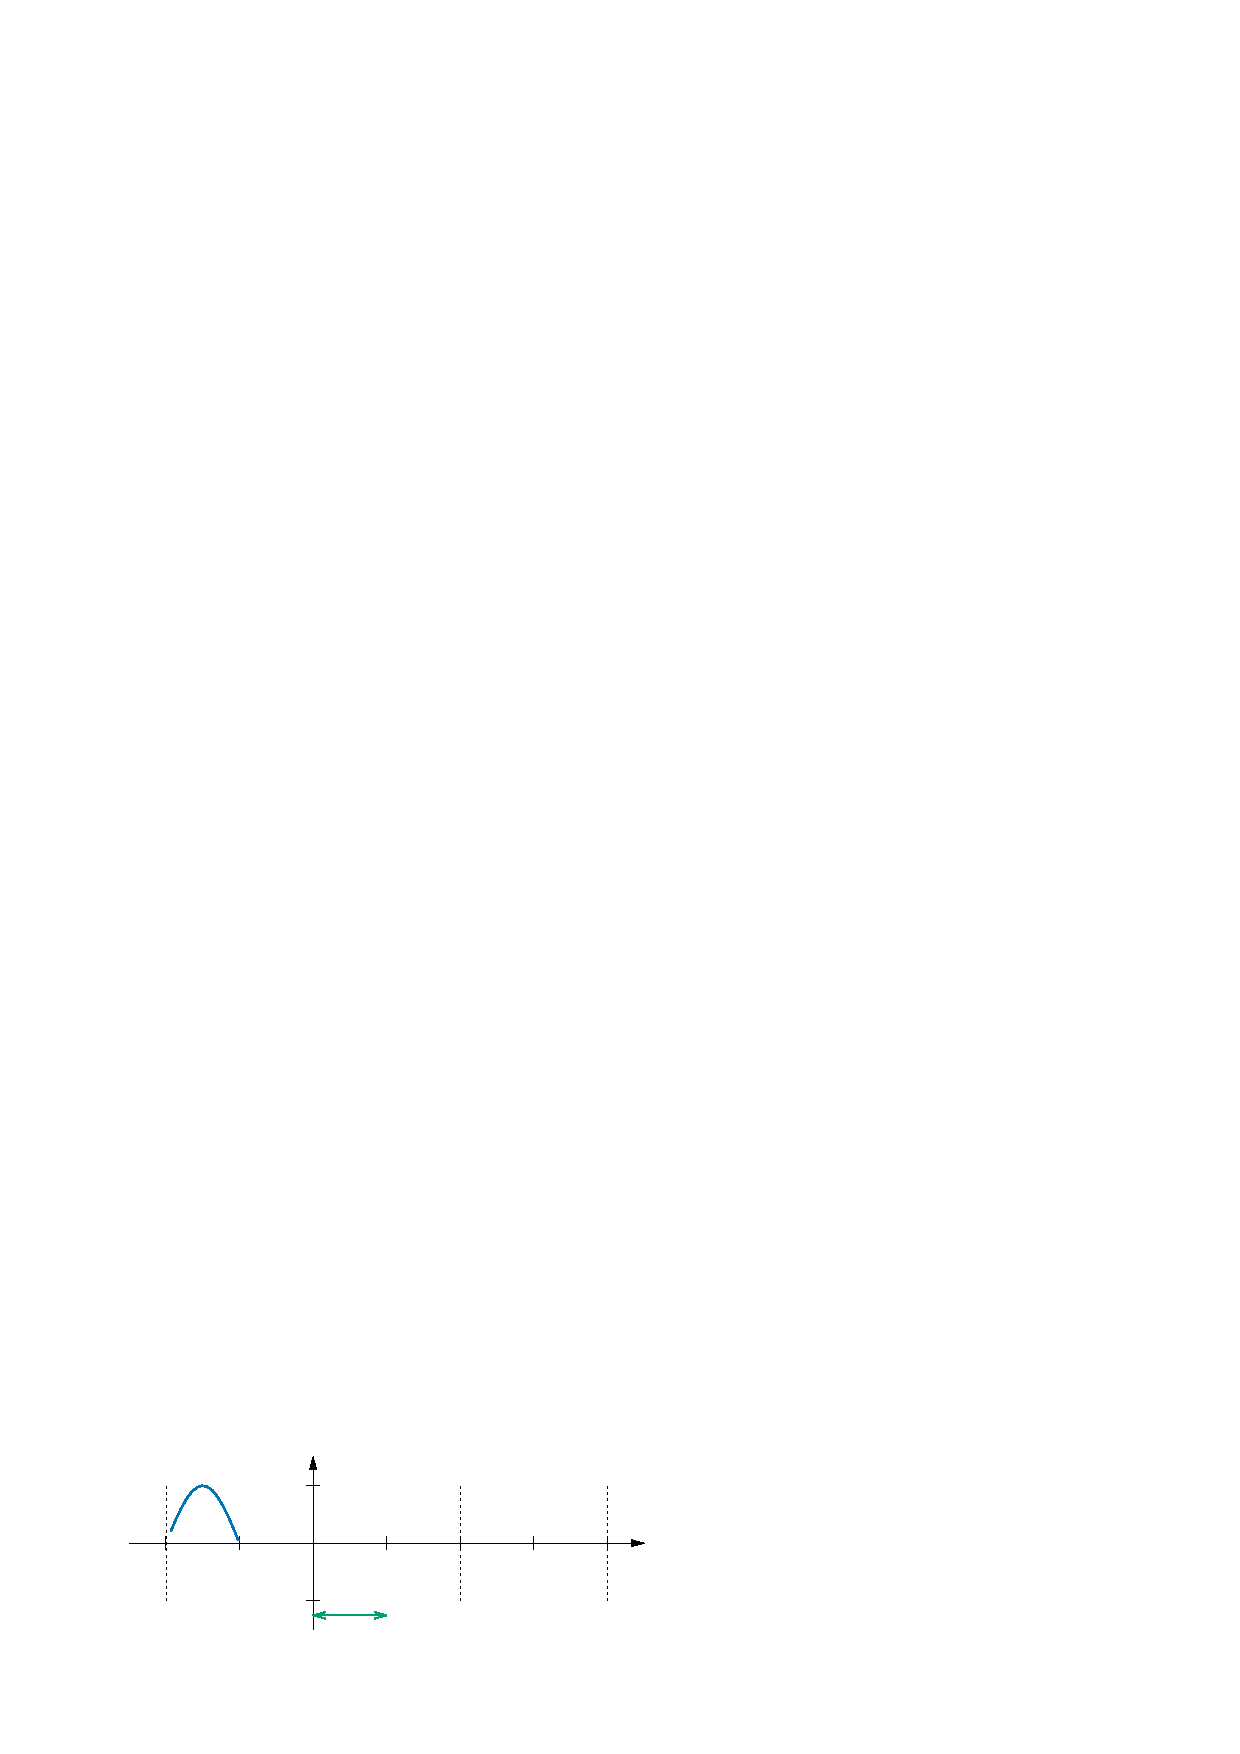
\includegraphics[width={273.60bp},height={100.70bp}]{figura_03_04}}%
    \gplfronttext
  \end{picture}%
\endgroup

\end{figure}

El periodo de la onda rectificada es la mitad del periodo de la onda original.

\section{Función escalón unitario}
\begin{equation}
    u(t)=\begin{cases}
        0&t<0\\
        1&t>0\\
    \end{cases}
\end{equation}
\begin{figure}[H]
    \centering
    % GNUPLOT: LaTeX picture with Postscript
\begingroup
  \makeatletter
  \providecommand\color[2][]{%
    \GenericError{(gnuplot) \space\space\space\@spaces}{%
      Package color not loaded in conjunction with
      terminal option `colourtext'%
    }{See the gnuplot documentation for explanation.%
    }{Either use 'blacktext' in gnuplot or load the package
      color.sty in LaTeX.}%
    \renewcommand\color[2][]{}%
  }%
  \providecommand\includegraphics[2][]{%
    \GenericError{(gnuplot) \space\space\space\@spaces}{%
      Package graphicx or graphics not loaded%
    }{See the gnuplot documentation for explanation.%
    }{The gnuplot epslatex terminal needs graphicx.sty or graphics.sty.}%
    \renewcommand\includegraphics[2][]{}%
  }%
  \providecommand\rotatebox[2]{#2}%
  \@ifundefined{ifGPcolor}{%
    \newif\ifGPcolor
    \GPcolorfalse
  }{}%
  \@ifundefined{ifGPblacktext}{%
    \newif\ifGPblacktext
    \GPblacktexttrue
  }{}%
  % define a \g@addto@macro without @ in the name:
  \let\gplgaddtomacro\g@addto@macro
  % define empty templates for all commands taking text:
  \gdef\gplbacktext{}%
  \gdef\gplfronttext{}%
  \makeatother
  \ifGPblacktext
    % no textcolor at all
    \def\colorrgb#1{}%
    \def\colorgray#1{}%
  \else
    % gray or color?
    \ifGPcolor
      \def\colorrgb#1{\color[rgb]{#1}}%
      \def\colorgray#1{\color[gray]{#1}}%
      \expandafter\def\csname LTw\endcsname{\color{white}}%
      \expandafter\def\csname LTb\endcsname{\color{black}}%
      \expandafter\def\csname LTa\endcsname{\color{black}}%
      \expandafter\def\csname LT0\endcsname{\color[rgb]{1,0,0}}%
      \expandafter\def\csname LT1\endcsname{\color[rgb]{0,1,0}}%
      \expandafter\def\csname LT2\endcsname{\color[rgb]{0,0,1}}%
      \expandafter\def\csname LT3\endcsname{\color[rgb]{1,0,1}}%
      \expandafter\def\csname LT4\endcsname{\color[rgb]{0,1,1}}%
      \expandafter\def\csname LT5\endcsname{\color[rgb]{1,1,0}}%
      \expandafter\def\csname LT6\endcsname{\color[rgb]{0,0,0}}%
      \expandafter\def\csname LT7\endcsname{\color[rgb]{1,0.3,0}}%
      \expandafter\def\csname LT8\endcsname{\color[rgb]{0.5,0.5,0.5}}%
    \else
      % gray
      \def\colorrgb#1{\color{black}}%
      \def\colorgray#1{\color[gray]{#1}}%
      \expandafter\def\csname LTw\endcsname{\color{white}}%
      \expandafter\def\csname LTb\endcsname{\color{black}}%
      \expandafter\def\csname LTa\endcsname{\color{black}}%
      \expandafter\def\csname LT0\endcsname{\color{black}}%
      \expandafter\def\csname LT1\endcsname{\color{black}}%
      \expandafter\def\csname LT2\endcsname{\color{black}}%
      \expandafter\def\csname LT3\endcsname{\color{black}}%
      \expandafter\def\csname LT4\endcsname{\color{black}}%
      \expandafter\def\csname LT5\endcsname{\color{black}}%
      \expandafter\def\csname LT6\endcsname{\color{black}}%
      \expandafter\def\csname LT7\endcsname{\color{black}}%
      \expandafter\def\csname LT8\endcsname{\color{black}}%
    \fi
  \fi
    \setlength{\unitlength}{0.0500bp}%
    \ifx\gptboxheight\undefined%
      \newlength{\gptboxheight}%
      \newlength{\gptboxwidth}%
      \newsavebox{\gptboxtext}%
    \fi%
    \setlength{\fboxrule}{0.5pt}%
    \setlength{\fboxsep}{1pt}%
    \definecolor{tbcol}{rgb}{1,1,1}%
\begin{picture}(5760.00,1440.00)%
    \gplgaddtomacro\gplbacktext{%
      \csname LTb\endcsname%%
      \put(2760,464){\makebox(0,0)[r]{\strut{}}}%
      \put(2760,1007){\makebox(0,0)[r]{\strut{}}}%
      \put(240,241){\makebox(0,0){\strut{}}}%
      \put(763,241){\makebox(0,0){\strut{}}}%
      \put(1286,241){\makebox(0,0){\strut{}}}%
      \put(1809,241){\makebox(0,0){\strut{}}}%
      \put(2332,241){\makebox(0,0){\strut{}}}%
      \put(2856,241){\makebox(0,0){\strut{}}}%
      \put(3379,241){\makebox(0,0){\strut{}}}%
      \put(3902,241){\makebox(0,0){\strut{}}}%
      \put(4425,241){\makebox(0,0){\strut{}}}%
      \put(4948,241){\makebox(0,0){\strut{}}}%
      \put(5471,241){\makebox(0,0){\strut{}}}%
      \csname LTb\endcsname%%
      \put(6256,464){\makebox(0,0)[l]{\strut{}$t$}}%
      \put(2751,1496){\makebox(0,0)[l]{\strut{}$f(t)$}}%
      \put(2594,1007){\makebox(0,0)[l]{\strut{}$1$}}%
    }%
    \gplgaddtomacro\gplfronttext{%
    }%
    \gplbacktext
    \put(0,0){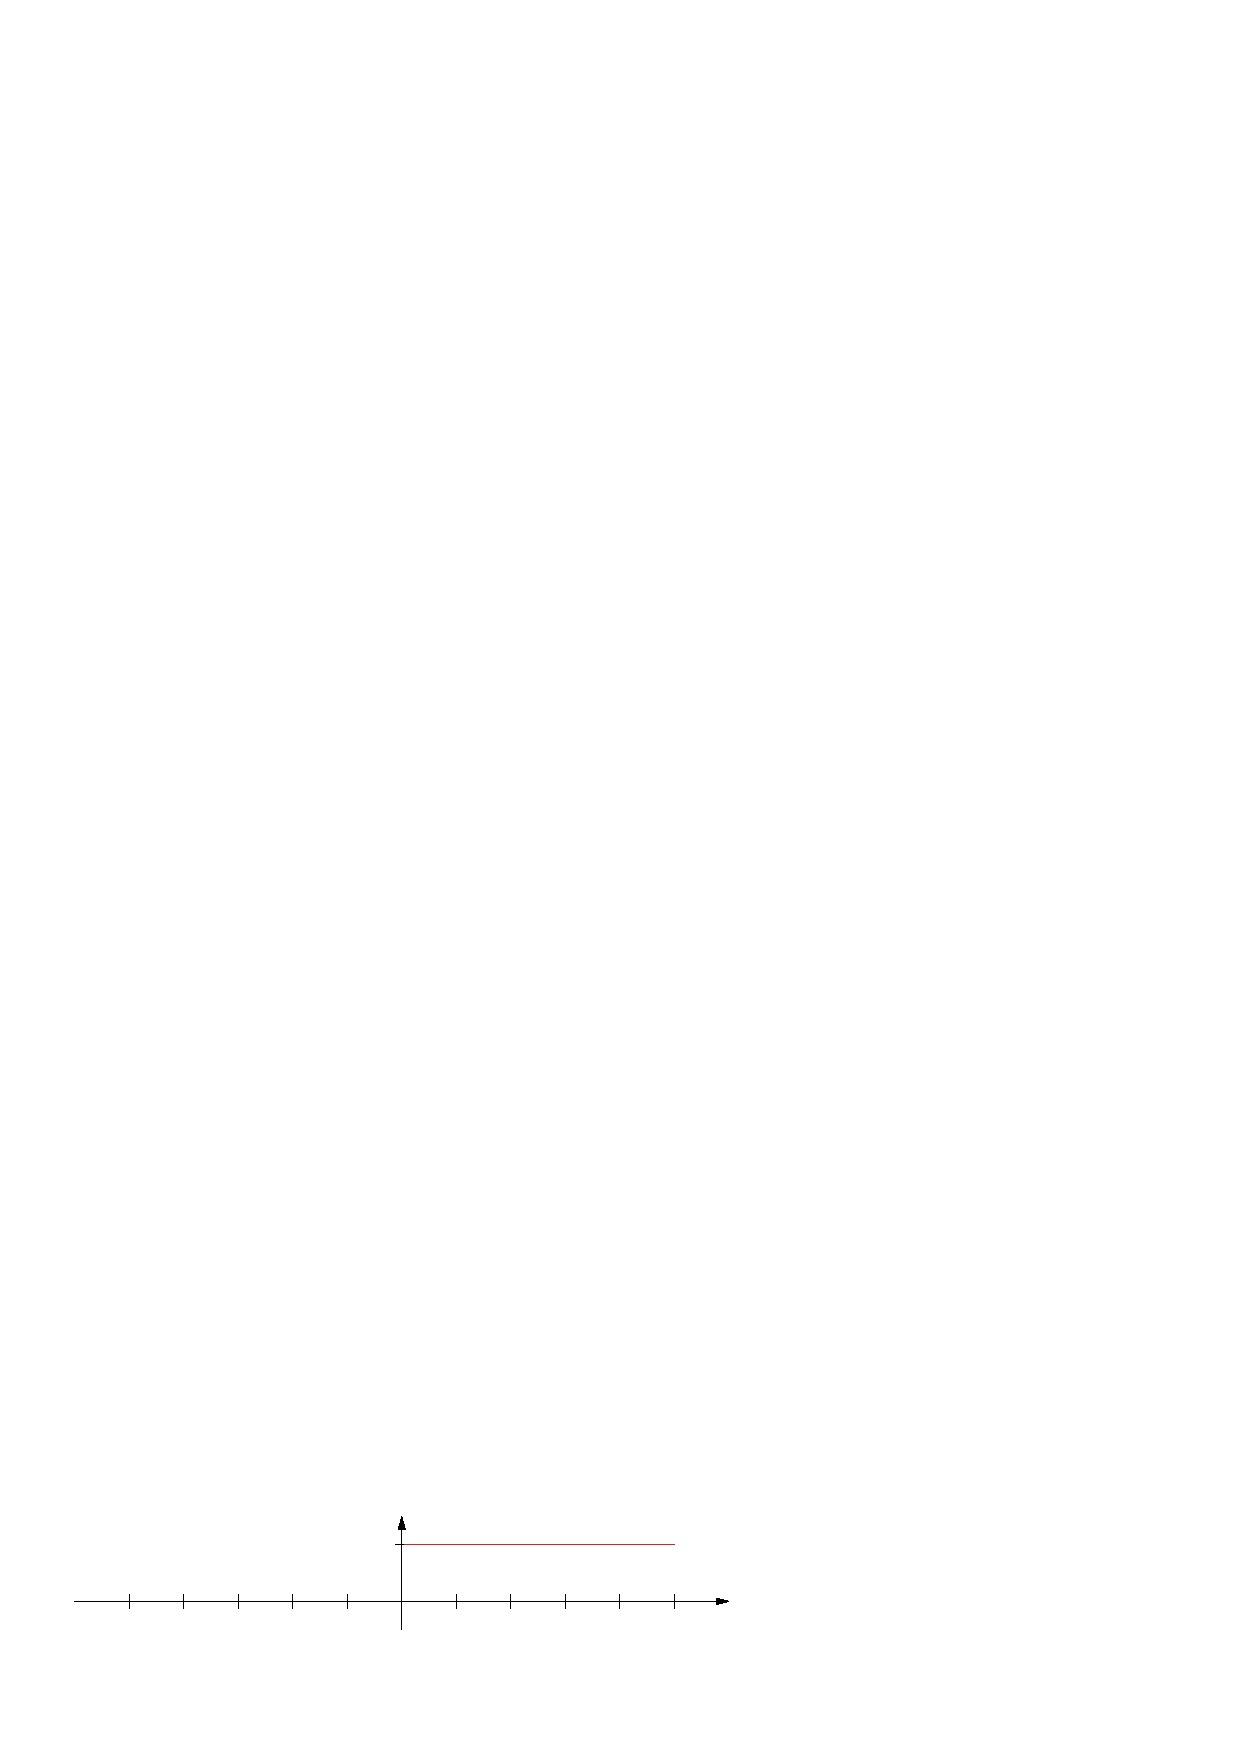
\includegraphics[width={288.00bp},height={72.00bp}]{figura_03_05}}%
    \gplfronttext
  \end{picture}%
\endgroup

\end{figure}

Una variante es:
\begin{equation*}
    u(-t)=\begin{cases}
        1&t<0\\
        0&t>0\\
    \end{cases}
\end{equation*}
\begin{figure}[H]
    \centering
    % GNUPLOT: LaTeX picture with Postscript
\begingroup
  \makeatletter
  \providecommand\color[2][]{%
    \GenericError{(gnuplot) \space\space\space\@spaces}{%
      Package color not loaded in conjunction with
      terminal option `colourtext'%
    }{See the gnuplot documentation for explanation.%
    }{Either use 'blacktext' in gnuplot or load the package
      color.sty in LaTeX.}%
    \renewcommand\color[2][]{}%
  }%
  \providecommand\includegraphics[2][]{%
    \GenericError{(gnuplot) \space\space\space\@spaces}{%
      Package graphicx or graphics not loaded%
    }{See the gnuplot documentation for explanation.%
    }{The gnuplot epslatex terminal needs graphicx.sty or graphics.sty.}%
    \renewcommand\includegraphics[2][]{}%
  }%
  \providecommand\rotatebox[2]{#2}%
  \@ifundefined{ifGPcolor}{%
    \newif\ifGPcolor
    \GPcolorfalse
  }{}%
  \@ifundefined{ifGPblacktext}{%
    \newif\ifGPblacktext
    \GPblacktexttrue
  }{}%
  % define a \g@addto@macro without @ in the name:
  \let\gplgaddtomacro\g@addto@macro
  % define empty templates for all commands taking text:
  \gdef\gplbacktext{}%
  \gdef\gplfronttext{}%
  \makeatother
  \ifGPblacktext
    % no textcolor at all
    \def\colorrgb#1{}%
    \def\colorgray#1{}%
  \else
    % gray or color?
    \ifGPcolor
      \def\colorrgb#1{\color[rgb]{#1}}%
      \def\colorgray#1{\color[gray]{#1}}%
      \expandafter\def\csname LTw\endcsname{\color{white}}%
      \expandafter\def\csname LTb\endcsname{\color{black}}%
      \expandafter\def\csname LTa\endcsname{\color{black}}%
      \expandafter\def\csname LT0\endcsname{\color[rgb]{1,0,0}}%
      \expandafter\def\csname LT1\endcsname{\color[rgb]{0,1,0}}%
      \expandafter\def\csname LT2\endcsname{\color[rgb]{0,0,1}}%
      \expandafter\def\csname LT3\endcsname{\color[rgb]{1,0,1}}%
      \expandafter\def\csname LT4\endcsname{\color[rgb]{0,1,1}}%
      \expandafter\def\csname LT5\endcsname{\color[rgb]{1,1,0}}%
      \expandafter\def\csname LT6\endcsname{\color[rgb]{0,0,0}}%
      \expandafter\def\csname LT7\endcsname{\color[rgb]{1,0.3,0}}%
      \expandafter\def\csname LT8\endcsname{\color[rgb]{0.5,0.5,0.5}}%
    \else
      % gray
      \def\colorrgb#1{\color{black}}%
      \def\colorgray#1{\color[gray]{#1}}%
      \expandafter\def\csname LTw\endcsname{\color{white}}%
      \expandafter\def\csname LTb\endcsname{\color{black}}%
      \expandafter\def\csname LTa\endcsname{\color{black}}%
      \expandafter\def\csname LT0\endcsname{\color{black}}%
      \expandafter\def\csname LT1\endcsname{\color{black}}%
      \expandafter\def\csname LT2\endcsname{\color{black}}%
      \expandafter\def\csname LT3\endcsname{\color{black}}%
      \expandafter\def\csname LT4\endcsname{\color{black}}%
      \expandafter\def\csname LT5\endcsname{\color{black}}%
      \expandafter\def\csname LT6\endcsname{\color{black}}%
      \expandafter\def\csname LT7\endcsname{\color{black}}%
      \expandafter\def\csname LT8\endcsname{\color{black}}%
    \fi
  \fi
    \setlength{\unitlength}{0.0500bp}%
    \ifx\gptboxheight\undefined%
      \newlength{\gptboxheight}%
      \newlength{\gptboxwidth}%
      \newsavebox{\gptboxtext}%
    \fi%
    \setlength{\fboxrule}{0.5pt}%
    \setlength{\fboxsep}{1pt}%
    \definecolor{tbcol}{rgb}{1,1,1}%
\begin{picture}(5760.00,1440.00)%
    \gplgaddtomacro\gplbacktext{%
      \csname LTb\endcsname%%
      \put(2760,464){\makebox(0,0)[r]{\strut{}}}%
      \put(2760,1007){\makebox(0,0)[r]{\strut{}}}%
      \put(240,241){\makebox(0,0){\strut{}}}%
      \put(763,241){\makebox(0,0){\strut{}}}%
      \put(1286,241){\makebox(0,0){\strut{}}}%
      \put(1809,241){\makebox(0,0){\strut{}}}%
      \put(2332,241){\makebox(0,0){\strut{}}}%
      \put(2856,241){\makebox(0,0){\strut{}}}%
      \put(3379,241){\makebox(0,0){\strut{}}}%
      \put(3902,241){\makebox(0,0){\strut{}}}%
      \put(4425,241){\makebox(0,0){\strut{}}}%
      \put(4948,241){\makebox(0,0){\strut{}}}%
      \put(5471,241){\makebox(0,0){\strut{}}}%
      \csname LTb\endcsname%%
      \put(6256,464){\makebox(0,0)[l]{\strut{}$t$}}%
      \put(2751,1496){\makebox(0,0)[l]{\strut{}$f(t)$}}%
      \put(3012,1007){\makebox(0,0)[l]{\strut{}$1$}}%
    }%
    \gplgaddtomacro\gplfronttext{%
    }%
    \gplbacktext
    \put(0,0){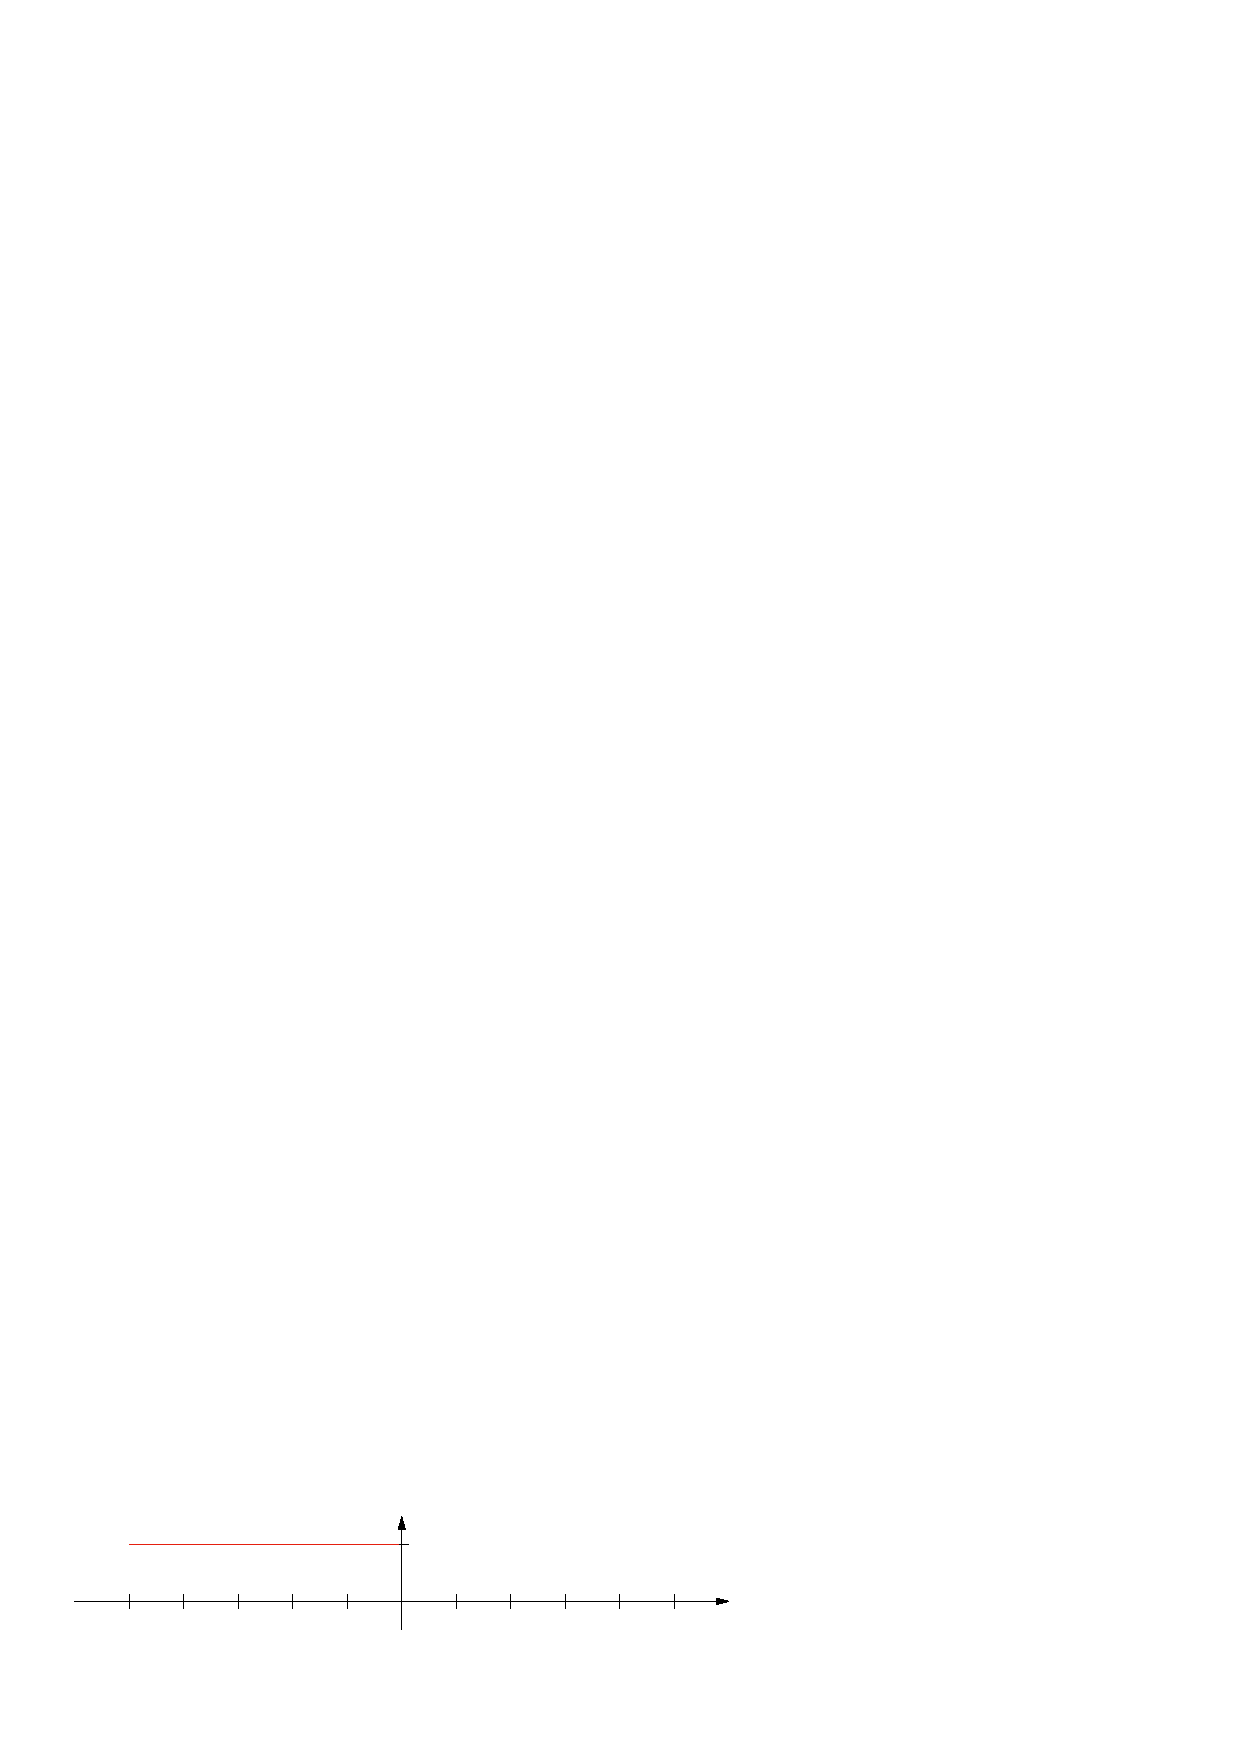
\includegraphics[width={288.00bp},height={72.00bp}]{figura_03_06}}%
    \gplfronttext
  \end{picture}%
\endgroup

\end{figure}

De manera general:
\begin{equation}
    k\,u(t-t_0)=\begin{cases}
        0&t<t_0\\
        k&t>t_0\\
    \end{cases}
\end{equation}
\begin{figure}[H]
    \centering
    % GNUPLOT: LaTeX picture with Postscript
\begingroup
  \makeatletter
  \providecommand\color[2][]{%
    \GenericError{(gnuplot) \space\space\space\@spaces}{%
      Package color not loaded in conjunction with
      terminal option `colourtext'%
    }{See the gnuplot documentation for explanation.%
    }{Either use 'blacktext' in gnuplot or load the package
      color.sty in LaTeX.}%
    \renewcommand\color[2][]{}%
  }%
  \providecommand\includegraphics[2][]{%
    \GenericError{(gnuplot) \space\space\space\@spaces}{%
      Package graphicx or graphics not loaded%
    }{See the gnuplot documentation for explanation.%
    }{The gnuplot epslatex terminal needs graphicx.sty or graphics.sty.}%
    \renewcommand\includegraphics[2][]{}%
  }%
  \providecommand\rotatebox[2]{#2}%
  \@ifundefined{ifGPcolor}{%
    \newif\ifGPcolor
    \GPcolorfalse
  }{}%
  \@ifundefined{ifGPblacktext}{%
    \newif\ifGPblacktext
    \GPblacktexttrue
  }{}%
  % define a \g@addto@macro without @ in the name:
  \let\gplgaddtomacro\g@addto@macro
  % define empty templates for all commands taking text:
  \gdef\gplbacktext{}%
  \gdef\gplfronttext{}%
  \makeatother
  \ifGPblacktext
    % no textcolor at all
    \def\colorrgb#1{}%
    \def\colorgray#1{}%
  \else
    % gray or color?
    \ifGPcolor
      \def\colorrgb#1{\color[rgb]{#1}}%
      \def\colorgray#1{\color[gray]{#1}}%
      \expandafter\def\csname LTw\endcsname{\color{white}}%
      \expandafter\def\csname LTb\endcsname{\color{black}}%
      \expandafter\def\csname LTa\endcsname{\color{black}}%
      \expandafter\def\csname LT0\endcsname{\color[rgb]{1,0,0}}%
      \expandafter\def\csname LT1\endcsname{\color[rgb]{0,1,0}}%
      \expandafter\def\csname LT2\endcsname{\color[rgb]{0,0,1}}%
      \expandafter\def\csname LT3\endcsname{\color[rgb]{1,0,1}}%
      \expandafter\def\csname LT4\endcsname{\color[rgb]{0,1,1}}%
      \expandafter\def\csname LT5\endcsname{\color[rgb]{1,1,0}}%
      \expandafter\def\csname LT6\endcsname{\color[rgb]{0,0,0}}%
      \expandafter\def\csname LT7\endcsname{\color[rgb]{1,0.3,0}}%
      \expandafter\def\csname LT8\endcsname{\color[rgb]{0.5,0.5,0.5}}%
    \else
      % gray
      \def\colorrgb#1{\color{black}}%
      \def\colorgray#1{\color[gray]{#1}}%
      \expandafter\def\csname LTw\endcsname{\color{white}}%
      \expandafter\def\csname LTb\endcsname{\color{black}}%
      \expandafter\def\csname LTa\endcsname{\color{black}}%
      \expandafter\def\csname LT0\endcsname{\color{black}}%
      \expandafter\def\csname LT1\endcsname{\color{black}}%
      \expandafter\def\csname LT2\endcsname{\color{black}}%
      \expandafter\def\csname LT3\endcsname{\color{black}}%
      \expandafter\def\csname LT4\endcsname{\color{black}}%
      \expandafter\def\csname LT5\endcsname{\color{black}}%
      \expandafter\def\csname LT6\endcsname{\color{black}}%
      \expandafter\def\csname LT7\endcsname{\color{black}}%
      \expandafter\def\csname LT8\endcsname{\color{black}}%
    \fi
  \fi
    \setlength{\unitlength}{0.0500bp}%
    \ifx\gptboxheight\undefined%
      \newlength{\gptboxheight}%
      \newlength{\gptboxwidth}%
      \newsavebox{\gptboxtext}%
    \fi%
    \setlength{\fboxrule}{0.5pt}%
    \setlength{\fboxsep}{1pt}%
    \definecolor{tbcol}{rgb}{1,1,1}%
\begin{picture}(5760.00,2160.00)%
    \gplgaddtomacro\gplbacktext{%
      \csname LTb\endcsname%%
      \put(2760,493){\makebox(0,0)[r]{\strut{}}}%
      \put(2760,1096){\makebox(0,0)[r]{\strut{}}}%
      \put(2760,1698){\makebox(0,0)[r]{\strut{}}}%
      \put(240,270){\makebox(0,0){\strut{}}}%
      \put(763,270){\makebox(0,0){\strut{}}}%
      \put(1286,270){\makebox(0,0){\strut{}}}%
      \put(1809,270){\makebox(0,0){\strut{}}}%
      \put(2332,270){\makebox(0,0){\strut{}}}%
      \put(2856,270){\makebox(0,0){\strut{}}}%
      \put(3379,270){\makebox(0,0){\strut{}}}%
      \put(3902,270){\makebox(0,0){\strut{}}}%
      \put(4425,270){\makebox(0,0){\strut{}}}%
      \put(4948,270){\makebox(0,0){\strut{}}}%
      \put(5471,270){\makebox(0,0){\strut{}}}%
      \csname LTb\endcsname%%
      \put(6256,493){\makebox(0,0)[l]{\strut{}$t$}}%
      \put(2751,2240){\makebox(0,0)[l]{\strut{}$f(t)$}}%
      \put(3588,312){\makebox(0,0)[l]{\strut{}$t_0$}}%
      \put(2594,1397){\makebox(0,0)[l]{\strut{}$k$}}%
    }%
    \gplgaddtomacro\gplfronttext{%
    }%
    \gplbacktext
    \put(0,0){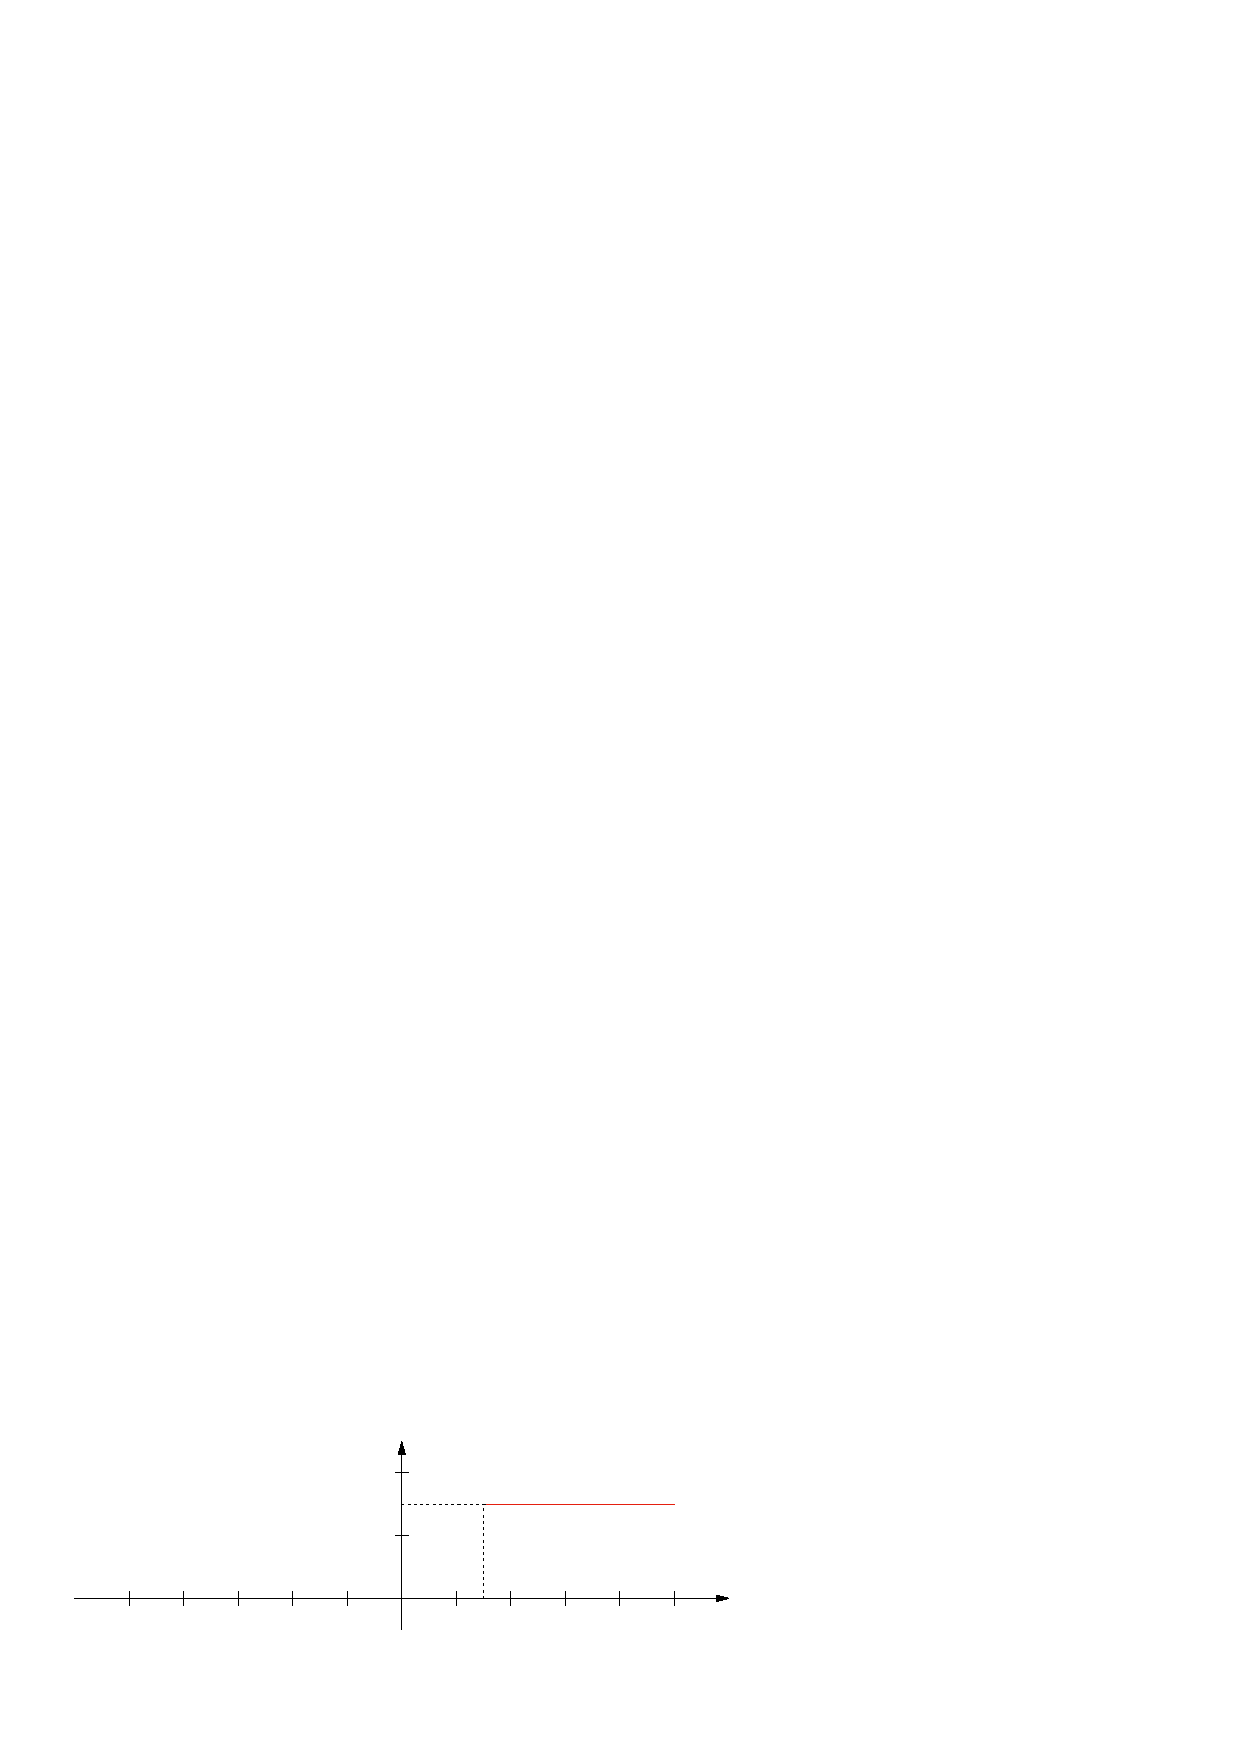
\includegraphics[width={288.00bp},height={108.00bp}]{figura_03_07}}%
    \gplfronttext
  \end{picture}%
\endgroup

\end{figure}

Si: $\phi(t)$ es una función de prueba:
\begin{figure}[H]
    \centering
    % GNUPLOT: LaTeX picture with Postscript
\begingroup
  \makeatletter
  \providecommand\color[2][]{%
    \GenericError{(gnuplot) \space\space\space\@spaces}{%
      Package color not loaded in conjunction with
      terminal option `colourtext'%
    }{See the gnuplot documentation for explanation.%
    }{Either use 'blacktext' in gnuplot or load the package
      color.sty in LaTeX.}%
    \renewcommand\color[2][]{}%
  }%
  \providecommand\includegraphics[2][]{%
    \GenericError{(gnuplot) \space\space\space\@spaces}{%
      Package graphicx or graphics not loaded%
    }{See the gnuplot documentation for explanation.%
    }{The gnuplot epslatex terminal needs graphicx.sty or graphics.sty.}%
    \renewcommand\includegraphics[2][]{}%
  }%
  \providecommand\rotatebox[2]{#2}%
  \@ifundefined{ifGPcolor}{%
    \newif\ifGPcolor
    \GPcolorfalse
  }{}%
  \@ifundefined{ifGPblacktext}{%
    \newif\ifGPblacktext
    \GPblacktexttrue
  }{}%
  % define a \g@addto@macro without @ in the name:
  \let\gplgaddtomacro\g@addto@macro
  % define empty templates for all commands taking text:
  \gdef\gplbacktext{}%
  \gdef\gplfronttext{}%
  \makeatother
  \ifGPblacktext
    % no textcolor at all
    \def\colorrgb#1{}%
    \def\colorgray#1{}%
  \else
    % gray or color?
    \ifGPcolor
      \def\colorrgb#1{\color[rgb]{#1}}%
      \def\colorgray#1{\color[gray]{#1}}%
      \expandafter\def\csname LTw\endcsname{\color{white}}%
      \expandafter\def\csname LTb\endcsname{\color{black}}%
      \expandafter\def\csname LTa\endcsname{\color{black}}%
      \expandafter\def\csname LT0\endcsname{\color[rgb]{1,0,0}}%
      \expandafter\def\csname LT1\endcsname{\color[rgb]{0,1,0}}%
      \expandafter\def\csname LT2\endcsname{\color[rgb]{0,0,1}}%
      \expandafter\def\csname LT3\endcsname{\color[rgb]{1,0,1}}%
      \expandafter\def\csname LT4\endcsname{\color[rgb]{0,1,1}}%
      \expandafter\def\csname LT5\endcsname{\color[rgb]{1,1,0}}%
      \expandafter\def\csname LT6\endcsname{\color[rgb]{0,0,0}}%
      \expandafter\def\csname LT7\endcsname{\color[rgb]{1,0.3,0}}%
      \expandafter\def\csname LT8\endcsname{\color[rgb]{0.5,0.5,0.5}}%
    \else
      % gray
      \def\colorrgb#1{\color{black}}%
      \def\colorgray#1{\color[gray]{#1}}%
      \expandafter\def\csname LTw\endcsname{\color{white}}%
      \expandafter\def\csname LTb\endcsname{\color{black}}%
      \expandafter\def\csname LTa\endcsname{\color{black}}%
      \expandafter\def\csname LT0\endcsname{\color{black}}%
      \expandafter\def\csname LT1\endcsname{\color{black}}%
      \expandafter\def\csname LT2\endcsname{\color{black}}%
      \expandafter\def\csname LT3\endcsname{\color{black}}%
      \expandafter\def\csname LT4\endcsname{\color{black}}%
      \expandafter\def\csname LT5\endcsname{\color{black}}%
      \expandafter\def\csname LT6\endcsname{\color{black}}%
      \expandafter\def\csname LT7\endcsname{\color{black}}%
      \expandafter\def\csname LT8\endcsname{\color{black}}%
    \fi
  \fi
    \setlength{\unitlength}{0.0500bp}%
    \ifx\gptboxheight\undefined%
      \newlength{\gptboxheight}%
      \newlength{\gptboxwidth}%
      \newsavebox{\gptboxtext}%
    \fi%
    \setlength{\fboxrule}{0.5pt}%
    \setlength{\fboxsep}{1pt}%
    \definecolor{tbcol}{rgb}{1,1,1}%
\begin{picture}(4320.00,2880.00)%
    \gplgaddtomacro\gplbacktext{%
      \csname LTb\endcsname%%
      \put(2040,192){\makebox(0,0)[r]{\strut{}}}%
      \put(2040,553){\makebox(0,0)[r]{\strut{}}}%
      \put(2040,914){\makebox(0,0)[r]{\strut{}}}%
      \put(2040,1275){\makebox(0,0)[r]{\strut{}}}%
      \put(2040,1636){\makebox(0,0)[r]{\strut{}}}%
      \put(2040,1997){\makebox(0,0)[r]{\strut{}}}%
      \put(2040,2358){\makebox(0,0)[r]{\strut{}}}%
      \put(2040,2719){\makebox(0,0)[r]{\strut{}}}%
      \put(240,330){\makebox(0,0){\strut{}}}%
      \put(714,330){\makebox(0,0){\strut{}}}%
      \put(1188,330){\makebox(0,0){\strut{}}}%
      \put(1662,330){\makebox(0,0){\strut{}}}%
      \put(2136,330){\makebox(0,0){\strut{}}}%
      \put(2609,330){\makebox(0,0){\strut{}}}%
      \put(3083,330){\makebox(0,0){\strut{}}}%
      \put(3557,330){\makebox(0,0){\strut{}}}%
      \put(4031,330){\makebox(0,0){\strut{}}}%
      \csname LTb\endcsname%%
      \put(4647,553){\makebox(0,0)[l]{\strut{}$t$}}%
      \put(2349,2863){\makebox(0,0)[l]{\strut{}$f(t)$}}%
      \put(2562,336){\makebox(0,0)[l]{\strut{}$t_0$}}%
      \put(1851,914){\makebox(0,0)[l]{\strut{}$1$}}%
      \put(714,2178){\makebox(0,0)[l]{\strut{}$\phi(t)$}}%
      \put(3083,1095){\makebox(0,0)[l]{\strut{}$u(t-t_0)$}}%
    }%
    \gplgaddtomacro\gplfronttext{%
    }%
    \gplgaddtomacro\gplbacktext{%
      \csname LTb\endcsname%%
      \put(2040,192){\makebox(0,0)[r]{\strut{}}}%
      \put(2040,553){\makebox(0,0)[r]{\strut{}}}%
      \put(2040,914){\makebox(0,0)[r]{\strut{}}}%
      \put(2040,1275){\makebox(0,0)[r]{\strut{}}}%
      \put(2040,1636){\makebox(0,0)[r]{\strut{}}}%
      \put(2040,1997){\makebox(0,0)[r]{\strut{}}}%
      \put(2040,2358){\makebox(0,0)[r]{\strut{}}}%
      \put(2040,2719){\makebox(0,0)[r]{\strut{}}}%
      \put(240,330){\makebox(0,0){\strut{}}}%
      \put(714,330){\makebox(0,0){\strut{}}}%
      \put(1188,330){\makebox(0,0){\strut{}}}%
      \put(1662,330){\makebox(0,0){\strut{}}}%
      \put(2136,330){\makebox(0,0){\strut{}}}%
      \put(2609,330){\makebox(0,0){\strut{}}}%
      \put(3083,330){\makebox(0,0){\strut{}}}%
      \put(3557,330){\makebox(0,0){\strut{}}}%
      \put(4031,330){\makebox(0,0){\strut{}}}%
      \csname LTb\endcsname%%
      \put(4647,553){\makebox(0,0)[l]{\strut{}$t$}}%
      \put(2349,2863){\makebox(0,0)[l]{\strut{}$f(t)$}}%
      \put(2562,336){\makebox(0,0)[l]{\strut{}$t_0$}}%
      \put(1851,914){\makebox(0,0)[l]{\strut{}$1$}}%
      \put(714,2178){\makebox(0,0)[l]{\strut{}$\phi(t)$}}%
      \put(3083,1095){\makebox(0,0)[l]{\strut{}$u(t-t_0)$}}%
    }%
    \gplgaddtomacro\gplfronttext{%
    }%
    \gplbacktext
    \put(0,0){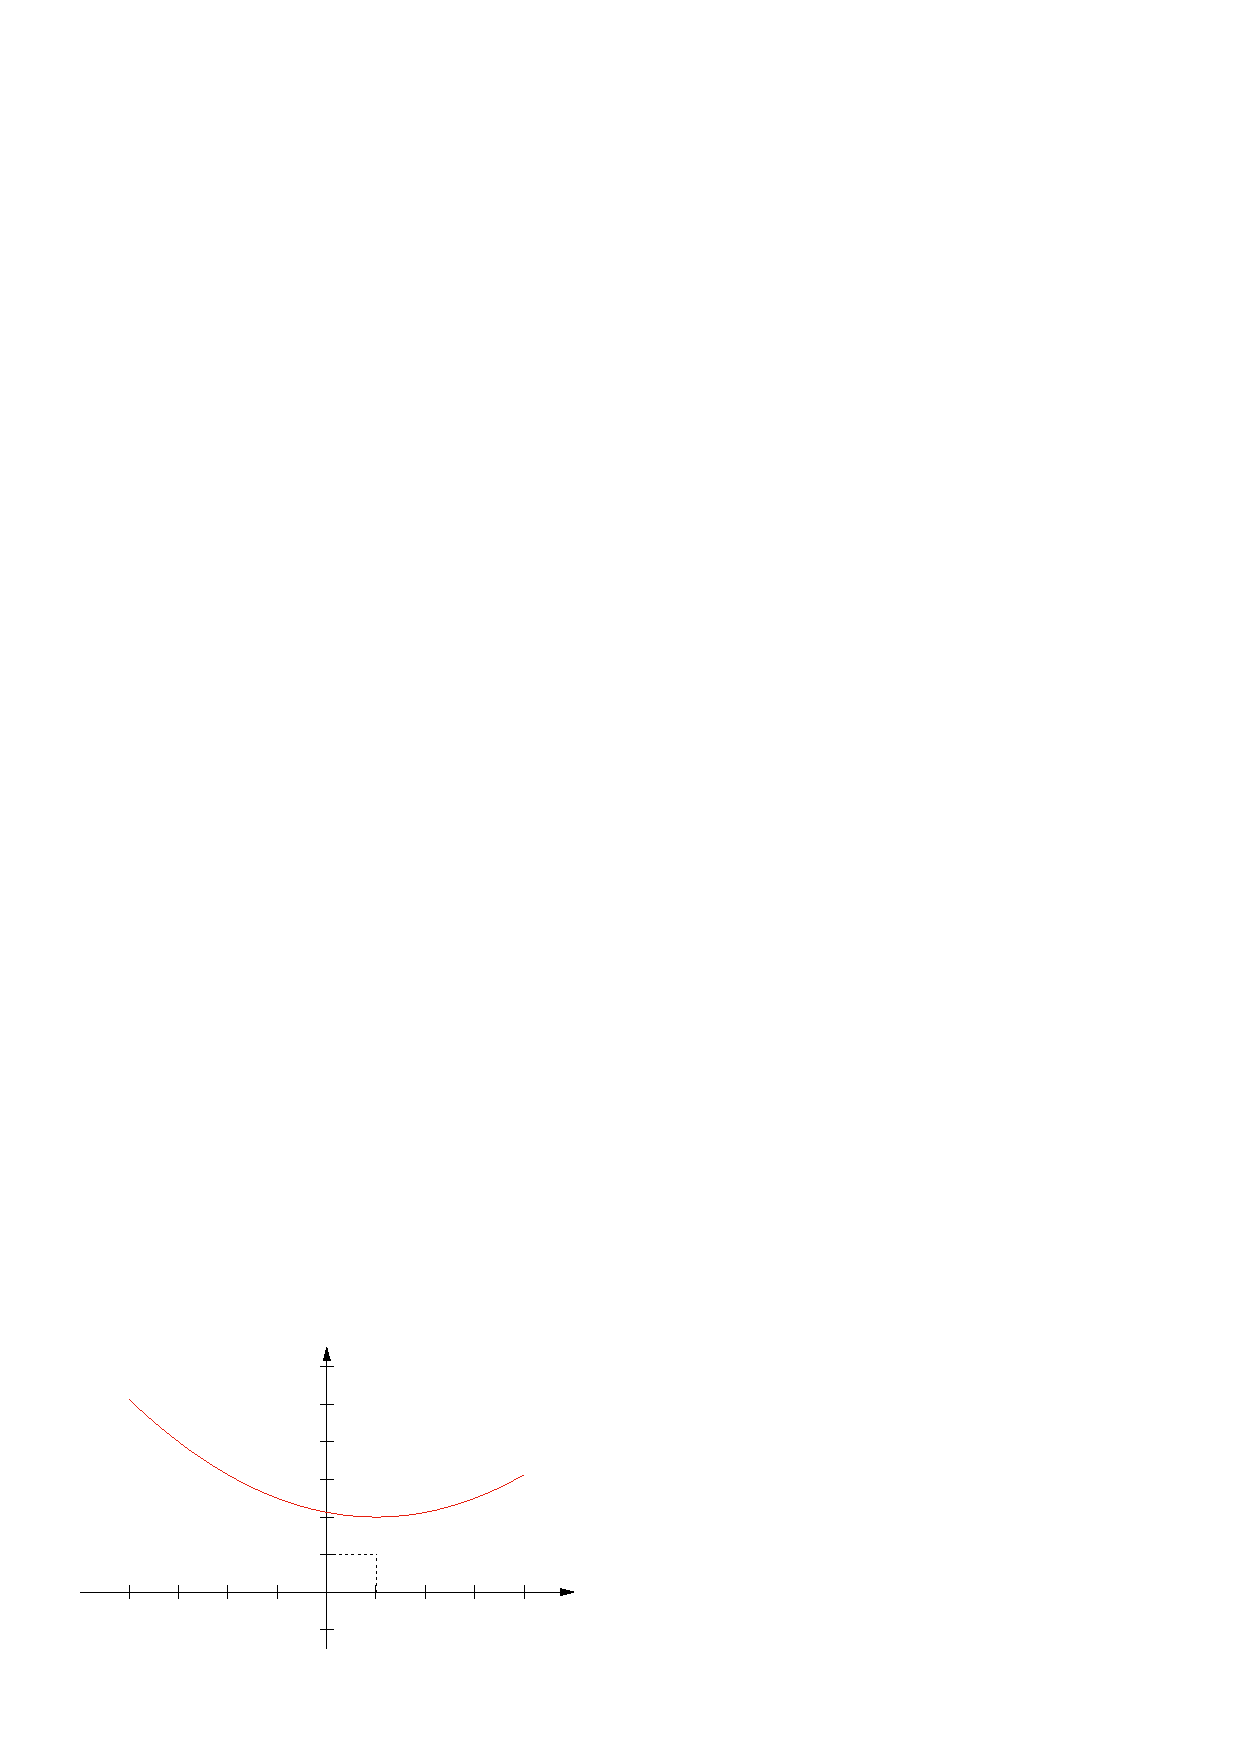
\includegraphics[width={216.00bp},height={144.00bp}]{figura_03_08}}%
    \gplfronttext
  \end{picture}%
\endgroup

\end{figure}
\begin{equation}
    \phi(t)u(t-t_0)=\begin{cases}
        0&t<t_0\\
        \phi(t)&t>t_0\\
    \end{cases}
\end{equation}
\begin{figure}[H]
    \centering
    % GNUPLOT: LaTeX picture with Postscript
\begingroup
  \makeatletter
  \providecommand\color[2][]{%
    \GenericError{(gnuplot) \space\space\space\@spaces}{%
      Package color not loaded in conjunction with
      terminal option `colourtext'%
    }{See the gnuplot documentation for explanation.%
    }{Either use 'blacktext' in gnuplot or load the package
      color.sty in LaTeX.}%
    \renewcommand\color[2][]{}%
  }%
  \providecommand\includegraphics[2][]{%
    \GenericError{(gnuplot) \space\space\space\@spaces}{%
      Package graphicx or graphics not loaded%
    }{See the gnuplot documentation for explanation.%
    }{The gnuplot epslatex terminal needs graphicx.sty or graphics.sty.}%
    \renewcommand\includegraphics[2][]{}%
  }%
  \providecommand\rotatebox[2]{#2}%
  \@ifundefined{ifGPcolor}{%
    \newif\ifGPcolor
    \GPcolorfalse
  }{}%
  \@ifundefined{ifGPblacktext}{%
    \newif\ifGPblacktext
    \GPblacktexttrue
  }{}%
  % define a \g@addto@macro without @ in the name:
  \let\gplgaddtomacro\g@addto@macro
  % define empty templates for all commands taking text:
  \gdef\gplbacktext{}%
  \gdef\gplfronttext{}%
  \makeatother
  \ifGPblacktext
    % no textcolor at all
    \def\colorrgb#1{}%
    \def\colorgray#1{}%
  \else
    % gray or color?
    \ifGPcolor
      \def\colorrgb#1{\color[rgb]{#1}}%
      \def\colorgray#1{\color[gray]{#1}}%
      \expandafter\def\csname LTw\endcsname{\color{white}}%
      \expandafter\def\csname LTb\endcsname{\color{black}}%
      \expandafter\def\csname LTa\endcsname{\color{black}}%
      \expandafter\def\csname LT0\endcsname{\color[rgb]{1,0,0}}%
      \expandafter\def\csname LT1\endcsname{\color[rgb]{0,1,0}}%
      \expandafter\def\csname LT2\endcsname{\color[rgb]{0,0,1}}%
      \expandafter\def\csname LT3\endcsname{\color[rgb]{1,0,1}}%
      \expandafter\def\csname LT4\endcsname{\color[rgb]{0,1,1}}%
      \expandafter\def\csname LT5\endcsname{\color[rgb]{1,1,0}}%
      \expandafter\def\csname LT6\endcsname{\color[rgb]{0,0,0}}%
      \expandafter\def\csname LT7\endcsname{\color[rgb]{1,0.3,0}}%
      \expandafter\def\csname LT8\endcsname{\color[rgb]{0.5,0.5,0.5}}%
    \else
      % gray
      \def\colorrgb#1{\color{black}}%
      \def\colorgray#1{\color[gray]{#1}}%
      \expandafter\def\csname LTw\endcsname{\color{white}}%
      \expandafter\def\csname LTb\endcsname{\color{black}}%
      \expandafter\def\csname LTa\endcsname{\color{black}}%
      \expandafter\def\csname LT0\endcsname{\color{black}}%
      \expandafter\def\csname LT1\endcsname{\color{black}}%
      \expandafter\def\csname LT2\endcsname{\color{black}}%
      \expandafter\def\csname LT3\endcsname{\color{black}}%
      \expandafter\def\csname LT4\endcsname{\color{black}}%
      \expandafter\def\csname LT5\endcsname{\color{black}}%
      \expandafter\def\csname LT6\endcsname{\color{black}}%
      \expandafter\def\csname LT7\endcsname{\color{black}}%
      \expandafter\def\csname LT8\endcsname{\color{black}}%
    \fi
  \fi
    \setlength{\unitlength}{0.0500bp}%
    \ifx\gptboxheight\undefined%
      \newlength{\gptboxheight}%
      \newlength{\gptboxwidth}%
      \newsavebox{\gptboxtext}%
    \fi%
    \setlength{\fboxrule}{0.5pt}%
    \setlength{\fboxsep}{1pt}%
    \definecolor{tbcol}{rgb}{1,1,1}%
\begin{picture}(4320.00,2880.00)%
    \gplgaddtomacro\gplbacktext{%
      \csname LTb\endcsname%%
      \put(2040,192){\makebox(0,0)[r]{\strut{}}}%
      \put(2040,553){\makebox(0,0)[r]{\strut{}}}%
      \put(2040,914){\makebox(0,0)[r]{\strut{}}}%
      \put(2040,1275){\makebox(0,0)[r]{\strut{}}}%
      \put(2040,1636){\makebox(0,0)[r]{\strut{}}}%
      \put(2040,1997){\makebox(0,0)[r]{\strut{}}}%
      \put(2040,2358){\makebox(0,0)[r]{\strut{}}}%
      \put(2040,2719){\makebox(0,0)[r]{\strut{}}}%
      \put(240,330){\makebox(0,0){\strut{}}}%
      \put(714,330){\makebox(0,0){\strut{}}}%
      \put(1188,330){\makebox(0,0){\strut{}}}%
      \put(1662,330){\makebox(0,0){\strut{}}}%
      \put(2136,330){\makebox(0,0){\strut{}}}%
      \put(2609,330){\makebox(0,0){\strut{}}}%
      \put(3083,330){\makebox(0,0){\strut{}}}%
      \put(3557,330){\makebox(0,0){\strut{}}}%
      \put(4031,330){\makebox(0,0){\strut{}}}%
      \csname LTb\endcsname%%
      \put(4647,553){\makebox(0,0)[l]{\strut{}$t$}}%
      \put(2349,2863){\makebox(0,0)[l]{\strut{}$f(t)$}}%
      \put(2562,336){\makebox(0,0)[l]{\strut{}$t_0$}}%
      \put(3083,1095){\makebox(0,0)[l]{\strut{}$\phi(t)u(t-t_0)$}}%
    }%
    \gplgaddtomacro\gplfronttext{%
    }%
    \gplbacktext
    \put(0,0){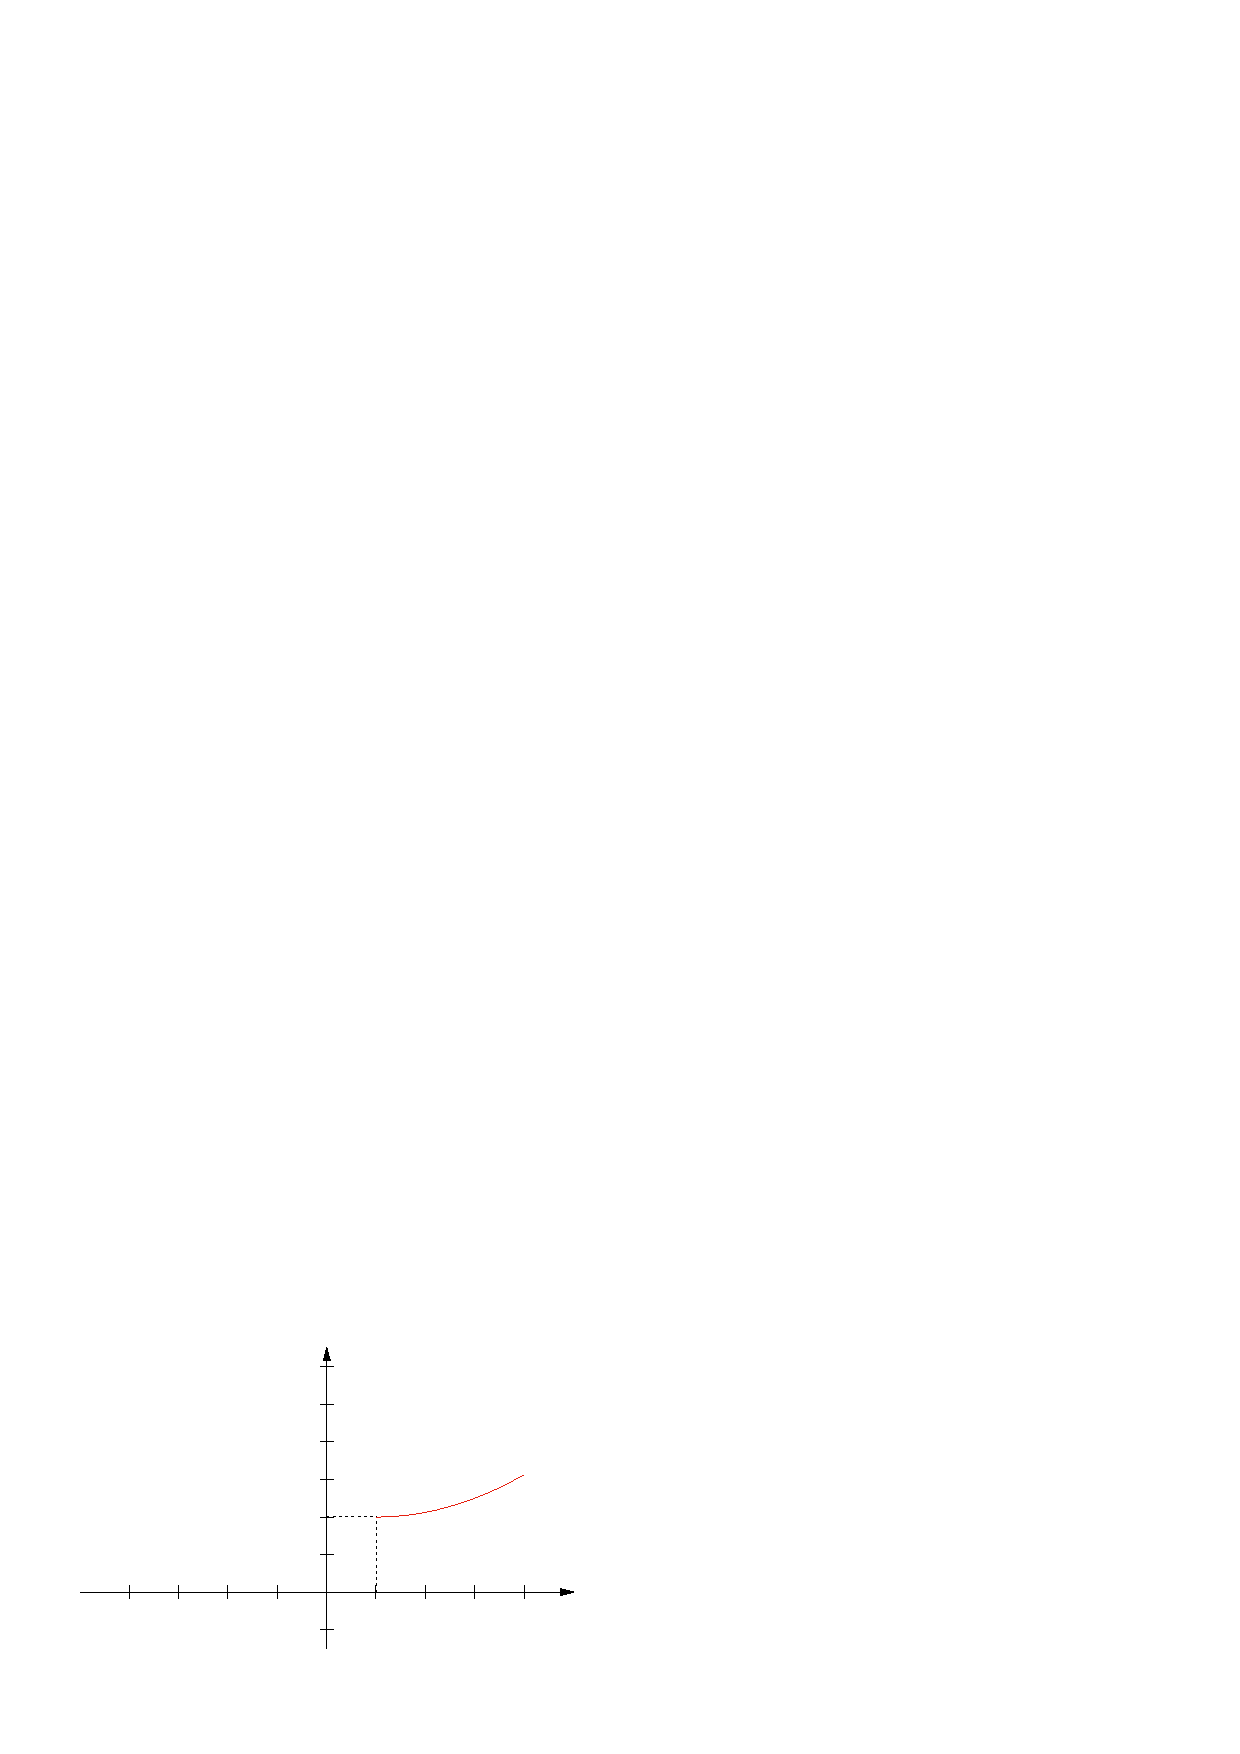
\includegraphics[width={216.00bp},height={144.00bp}]{figura_03_09}}%
    \gplfronttext
  \end{picture}%
\endgroup

\end{figure}
\begin{equation*}
    \phi(t)(u(t-t_1)-u(t-t_2))=\begin{cases}
        0&t\notin[t_1,t_2]\\
        \phi(t)&t\in[t_1,t_2]\\
    \end{cases}
\end{equation*}
\begin{figure}[H]
    \centering
    % GNUPLOT: LaTeX picture with Postscript
\begingroup
  \makeatletter
  \providecommand\color[2][]{%
    \GenericError{(gnuplot) \space\space\space\@spaces}{%
      Package color not loaded in conjunction with
      terminal option `colourtext'%
    }{See the gnuplot documentation for explanation.%
    }{Either use 'blacktext' in gnuplot or load the package
      color.sty in LaTeX.}%
    \renewcommand\color[2][]{}%
  }%
  \providecommand\includegraphics[2][]{%
    \GenericError{(gnuplot) \space\space\space\@spaces}{%
      Package graphicx or graphics not loaded%
    }{See the gnuplot documentation for explanation.%
    }{The gnuplot epslatex terminal needs graphicx.sty or graphics.sty.}%
    \renewcommand\includegraphics[2][]{}%
  }%
  \providecommand\rotatebox[2]{#2}%
  \@ifundefined{ifGPcolor}{%
    \newif\ifGPcolor
    \GPcolorfalse
  }{}%
  \@ifundefined{ifGPblacktext}{%
    \newif\ifGPblacktext
    \GPblacktexttrue
  }{}%
  % define a \g@addto@macro without @ in the name:
  \let\gplgaddtomacro\g@addto@macro
  % define empty templates for all commands taking text:
  \gdef\gplbacktext{}%
  \gdef\gplfronttext{}%
  \makeatother
  \ifGPblacktext
    % no textcolor at all
    \def\colorrgb#1{}%
    \def\colorgray#1{}%
  \else
    % gray or color?
    \ifGPcolor
      \def\colorrgb#1{\color[rgb]{#1}}%
      \def\colorgray#1{\color[gray]{#1}}%
      \expandafter\def\csname LTw\endcsname{\color{white}}%
      \expandafter\def\csname LTb\endcsname{\color{black}}%
      \expandafter\def\csname LTa\endcsname{\color{black}}%
      \expandafter\def\csname LT0\endcsname{\color[rgb]{1,0,0}}%
      \expandafter\def\csname LT1\endcsname{\color[rgb]{0,1,0}}%
      \expandafter\def\csname LT2\endcsname{\color[rgb]{0,0,1}}%
      \expandafter\def\csname LT3\endcsname{\color[rgb]{1,0,1}}%
      \expandafter\def\csname LT4\endcsname{\color[rgb]{0,1,1}}%
      \expandafter\def\csname LT5\endcsname{\color[rgb]{1,1,0}}%
      \expandafter\def\csname LT6\endcsname{\color[rgb]{0,0,0}}%
      \expandafter\def\csname LT7\endcsname{\color[rgb]{1,0.3,0}}%
      \expandafter\def\csname LT8\endcsname{\color[rgb]{0.5,0.5,0.5}}%
    \else
      % gray
      \def\colorrgb#1{\color{black}}%
      \def\colorgray#1{\color[gray]{#1}}%
      \expandafter\def\csname LTw\endcsname{\color{white}}%
      \expandafter\def\csname LTb\endcsname{\color{black}}%
      \expandafter\def\csname LTa\endcsname{\color{black}}%
      \expandafter\def\csname LT0\endcsname{\color{black}}%
      \expandafter\def\csname LT1\endcsname{\color{black}}%
      \expandafter\def\csname LT2\endcsname{\color{black}}%
      \expandafter\def\csname LT3\endcsname{\color{black}}%
      \expandafter\def\csname LT4\endcsname{\color{black}}%
      \expandafter\def\csname LT5\endcsname{\color{black}}%
      \expandafter\def\csname LT6\endcsname{\color{black}}%
      \expandafter\def\csname LT7\endcsname{\color{black}}%
      \expandafter\def\csname LT8\endcsname{\color{black}}%
    \fi
  \fi
    \setlength{\unitlength}{0.0500bp}%
    \ifx\gptboxheight\undefined%
      \newlength{\gptboxheight}%
      \newlength{\gptboxwidth}%
      \newsavebox{\gptboxtext}%
    \fi%
    \setlength{\fboxrule}{0.5pt}%
    \setlength{\fboxsep}{1pt}%
    \definecolor{tbcol}{rgb}{1,1,1}%
\begin{picture}(4320.00,2880.00)%
    \gplgaddtomacro\gplbacktext{%
      \csname LTb\endcsname%%
      \put(2040,192){\makebox(0,0)[r]{\strut{}}}%
      \put(2040,553){\makebox(0,0)[r]{\strut{}}}%
      \put(2040,914){\makebox(0,0)[r]{\strut{}}}%
      \put(2040,1275){\makebox(0,0)[r]{\strut{}}}%
      \put(2040,1636){\makebox(0,0)[r]{\strut{}}}%
      \put(2040,1997){\makebox(0,0)[r]{\strut{}}}%
      \put(2040,2358){\makebox(0,0)[r]{\strut{}}}%
      \put(2040,2719){\makebox(0,0)[r]{\strut{}}}%
      \put(240,330){\makebox(0,0){\strut{}}}%
      \put(714,330){\makebox(0,0){\strut{}}}%
      \put(1188,330){\makebox(0,0){\strut{}}}%
      \put(1662,330){\makebox(0,0){\strut{}}}%
      \put(2136,330){\makebox(0,0){\strut{}}}%
      \put(2609,330){\makebox(0,0){\strut{}}}%
      \put(3083,330){\makebox(0,0){\strut{}}}%
      \put(3557,330){\makebox(0,0){\strut{}}}%
      \put(4031,330){\makebox(0,0){\strut{}}}%
      \csname LTb\endcsname%%
      \put(4647,553){\makebox(0,0)[l]{\strut{}$t$}}%
      \put(2349,2863){\makebox(0,0)[l]{\strut{}$f(t)$}}%
      \put(2562,336){\makebox(0,0)[l]{\strut{}$t_1$}}%
      \put(3510,336){\makebox(0,0)[l]{\strut{}$t_2$}}%
      \put(2609,1817){\makebox(0,0)[l]{\strut{}$\phi(t)(u(t-t_1)-u(t-t_2))$}}%
    }%
    \gplgaddtomacro\gplfronttext{%
    }%
    \gplbacktext
    \put(0,0){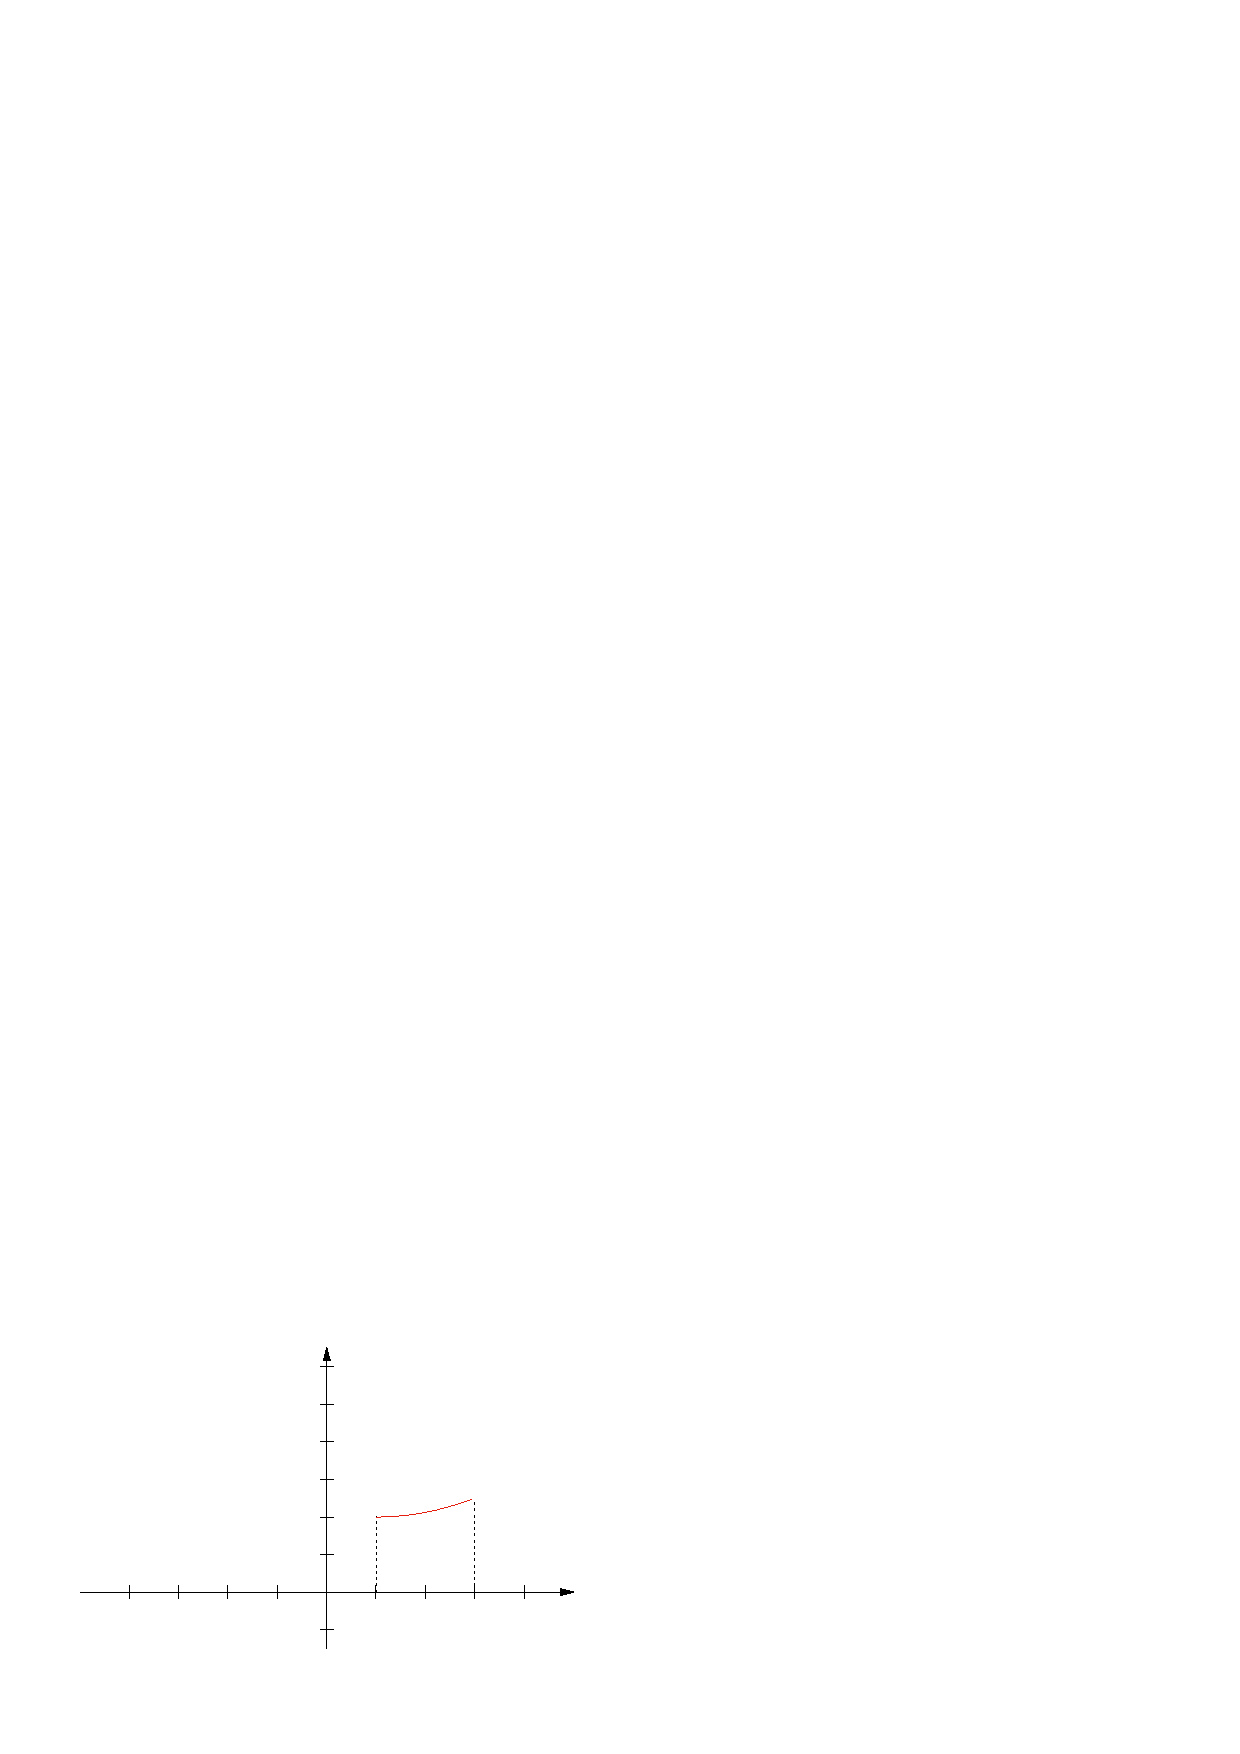
\includegraphics[width={216.00bp},height={144.00bp}]{figura_03_10}}%
    \gplfronttext
  \end{picture}%
\endgroup

\end{figure}

\section{La función impulso}
Pulso rectangular de área igual a 1.
\begin{figure}[H]
    \centering
    % GNUPLOT: LaTeX picture with Postscript
\begingroup
  \makeatletter
  \providecommand\color[2][]{%
    \GenericError{(gnuplot) \space\space\space\@spaces}{%
      Package color not loaded in conjunction with
      terminal option `colourtext'%
    }{See the gnuplot documentation for explanation.%
    }{Either use 'blacktext' in gnuplot or load the package
      color.sty in LaTeX.}%
    \renewcommand\color[2][]{}%
  }%
  \providecommand\includegraphics[2][]{%
    \GenericError{(gnuplot) \space\space\space\@spaces}{%
      Package graphicx or graphics not loaded%
    }{See the gnuplot documentation for explanation.%
    }{The gnuplot epslatex terminal needs graphicx.sty or graphics.sty.}%
    \renewcommand\includegraphics[2][]{}%
  }%
  \providecommand\rotatebox[2]{#2}%
  \@ifundefined{ifGPcolor}{%
    \newif\ifGPcolor
    \GPcolorfalse
  }{}%
  \@ifundefined{ifGPblacktext}{%
    \newif\ifGPblacktext
    \GPblacktexttrue
  }{}%
  % define a \g@addto@macro without @ in the name:
  \let\gplgaddtomacro\g@addto@macro
  % define empty templates for all commands taking text:
  \gdef\gplbacktext{}%
  \gdef\gplfronttext{}%
  \makeatother
  \ifGPblacktext
    % no textcolor at all
    \def\colorrgb#1{}%
    \def\colorgray#1{}%
  \else
    % gray or color?
    \ifGPcolor
      \def\colorrgb#1{\color[rgb]{#1}}%
      \def\colorgray#1{\color[gray]{#1}}%
      \expandafter\def\csname LTw\endcsname{\color{white}}%
      \expandafter\def\csname LTb\endcsname{\color{black}}%
      \expandafter\def\csname LTa\endcsname{\color{black}}%
      \expandafter\def\csname LT0\endcsname{\color[rgb]{1,0,0}}%
      \expandafter\def\csname LT1\endcsname{\color[rgb]{0,1,0}}%
      \expandafter\def\csname LT2\endcsname{\color[rgb]{0,0,1}}%
      \expandafter\def\csname LT3\endcsname{\color[rgb]{1,0,1}}%
      \expandafter\def\csname LT4\endcsname{\color[rgb]{0,1,1}}%
      \expandafter\def\csname LT5\endcsname{\color[rgb]{1,1,0}}%
      \expandafter\def\csname LT6\endcsname{\color[rgb]{0,0,0}}%
      \expandafter\def\csname LT7\endcsname{\color[rgb]{1,0.3,0}}%
      \expandafter\def\csname LT8\endcsname{\color[rgb]{0.5,0.5,0.5}}%
    \else
      % gray
      \def\colorrgb#1{\color{black}}%
      \def\colorgray#1{\color[gray]{#1}}%
      \expandafter\def\csname LTw\endcsname{\color{white}}%
      \expandafter\def\csname LTb\endcsname{\color{black}}%
      \expandafter\def\csname LTa\endcsname{\color{black}}%
      \expandafter\def\csname LT0\endcsname{\color{black}}%
      \expandafter\def\csname LT1\endcsname{\color{black}}%
      \expandafter\def\csname LT2\endcsname{\color{black}}%
      \expandafter\def\csname LT3\endcsname{\color{black}}%
      \expandafter\def\csname LT4\endcsname{\color{black}}%
      \expandafter\def\csname LT5\endcsname{\color{black}}%
      \expandafter\def\csname LT6\endcsname{\color{black}}%
      \expandafter\def\csname LT7\endcsname{\color{black}}%
      \expandafter\def\csname LT8\endcsname{\color{black}}%
    \fi
  \fi
    \setlength{\unitlength}{0.0500bp}%
    \ifx\gptboxheight\undefined%
      \newlength{\gptboxheight}%
      \newlength{\gptboxwidth}%
      \newsavebox{\gptboxtext}%
    \fi%
    \setlength{\fboxrule}{0.5pt}%
    \setlength{\fboxsep}{1pt}%
    \definecolor{tbcol}{rgb}{1,1,1}%
\begin{picture}(2160.00,2160.00)%
    \gplgaddtomacro\gplbacktext{%
      \csname LTb\endcsname%%
      \put(960,192){\makebox(0,0)[r]{\strut{}}}%
      \put(960,644){\makebox(0,0)[r]{\strut{}}}%
      \put(960,1096){\makebox(0,0)[r]{\strut{}}}%
      \put(960,1547){\makebox(0,0)[r]{\strut{}}}%
      \put(960,1999){\makebox(0,0)[r]{\strut{}}}%
      \put(240,421){\makebox(0,0){\strut{}}}%
      \put(648,421){\makebox(0,0){\strut{}}}%
      \put(1056,421){\makebox(0,0){\strut{}}}%
      \put(1463,421){\makebox(0,0){\strut{}}}%
      \put(1871,421){\makebox(0,0){\strut{}}}%
      \csname LTb\endcsname%%
      \put(2279,644){\makebox(0,0)[l]{\strut{}$t$}}%
      \put(1239,2180){\makebox(0,0)[l]{\strut{}$f(t)$}}%
      \put(1422,373){\makebox(0,0)[l]{\strut{}$\xi$}}%
      \put(444,373){\makebox(0,0)[l]{\strut{}$-\xi$}}%
      \put(1626,1547){\makebox(0,0)[l]{\strut{}$\dfrac{1}{2\xi}$}}%
    }%
    \gplgaddtomacro\gplfronttext{%
    }%
    \gplbacktext
    \put(0,0){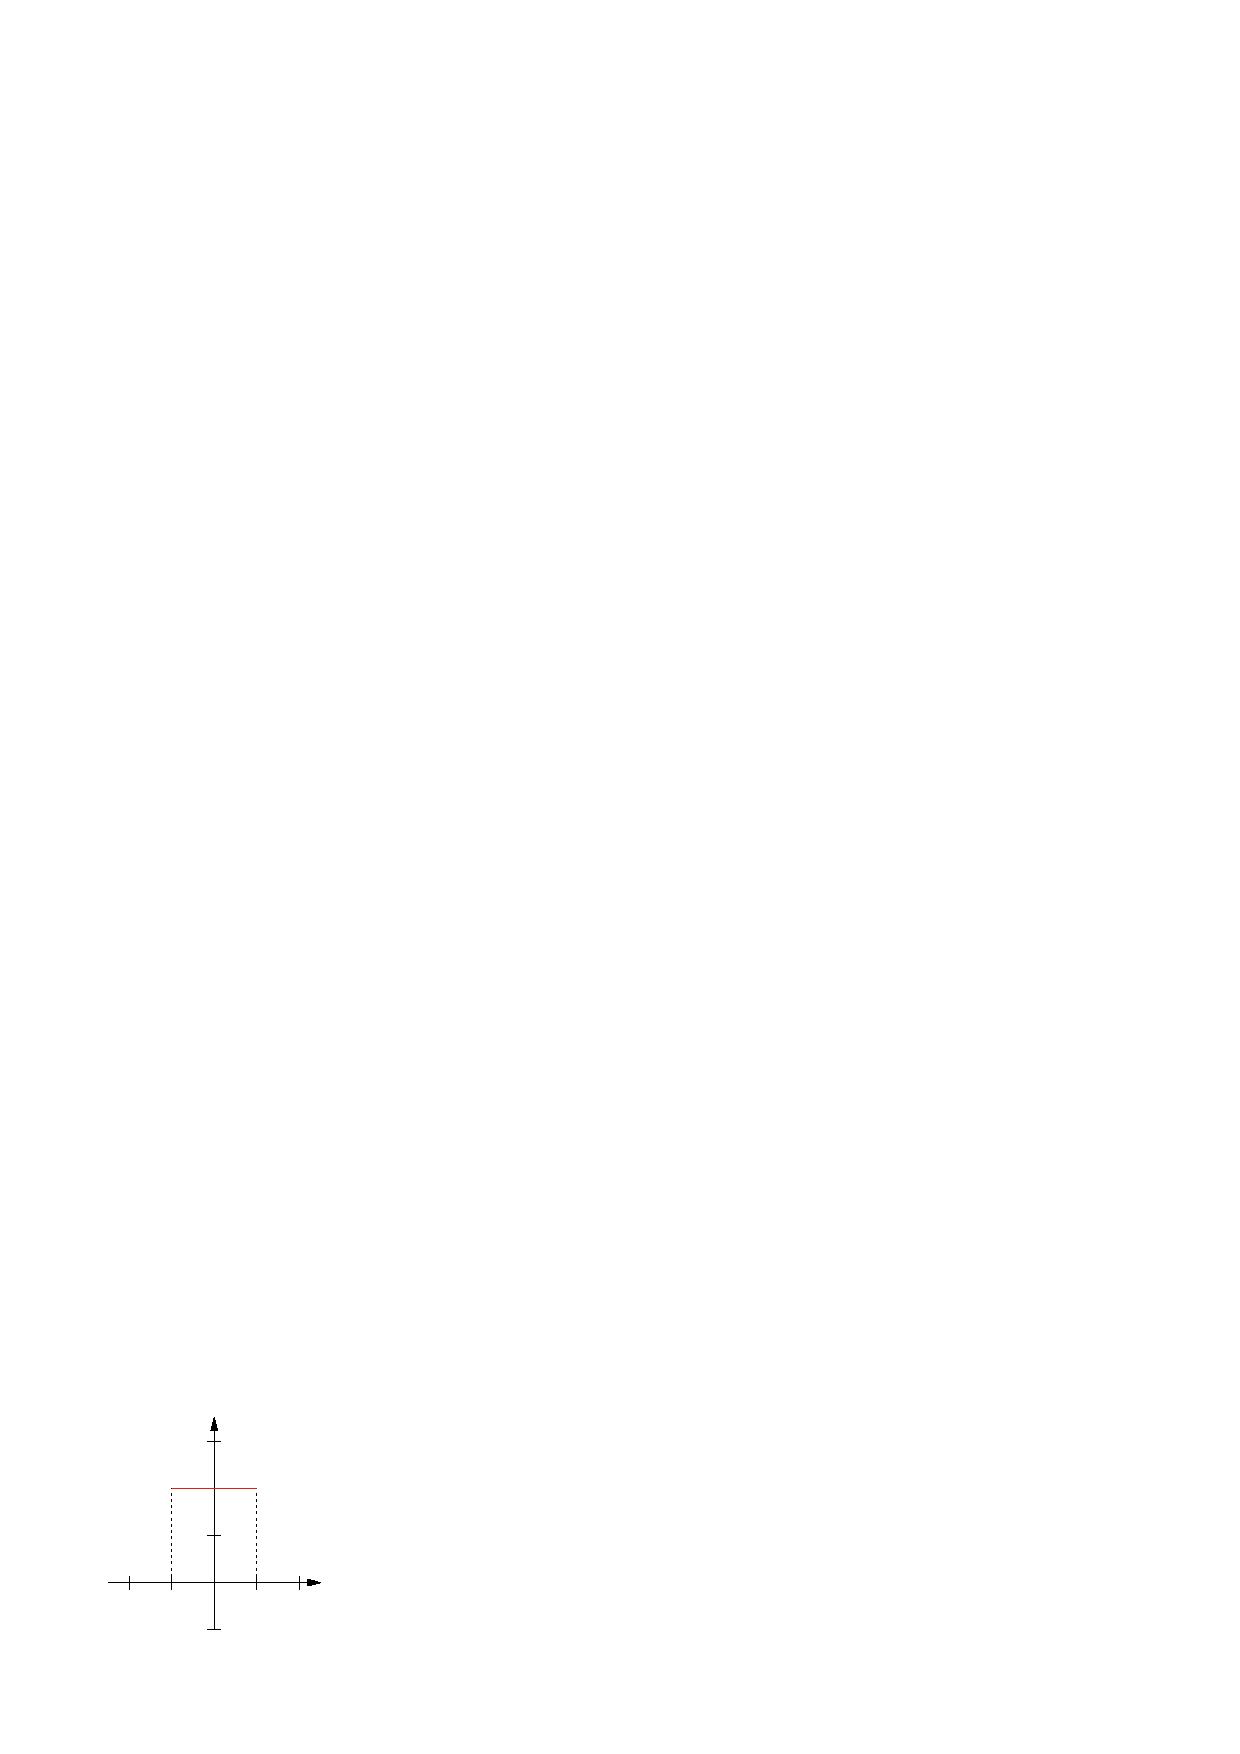
\includegraphics[width={108.00bp},height={108.00bp}]{figura_03_11}}%
    \gplfronttext
  \end{picture}%
\endgroup

\end{figure}

Si $\xi\to0$, entonces $\frac{1}{2\xi}\to\infty$.
\begin{figure}[H]
    \centering
    % GNUPLOT: LaTeX picture with Postscript
\begingroup
  \makeatletter
  \providecommand\color[2][]{%
    \GenericError{(gnuplot) \space\space\space\@spaces}{%
      Package color not loaded in conjunction with
      terminal option `colourtext'%
    }{See the gnuplot documentation for explanation.%
    }{Either use 'blacktext' in gnuplot or load the package
      color.sty in LaTeX.}%
    \renewcommand\color[2][]{}%
  }%
  \providecommand\includegraphics[2][]{%
    \GenericError{(gnuplot) \space\space\space\@spaces}{%
      Package graphicx or graphics not loaded%
    }{See the gnuplot documentation for explanation.%
    }{The gnuplot epslatex terminal needs graphicx.sty or graphics.sty.}%
    \renewcommand\includegraphics[2][]{}%
  }%
  \providecommand\rotatebox[2]{#2}%
  \@ifundefined{ifGPcolor}{%
    \newif\ifGPcolor
    \GPcolorfalse
  }{}%
  \@ifundefined{ifGPblacktext}{%
    \newif\ifGPblacktext
    \GPblacktexttrue
  }{}%
  % define a \g@addto@macro without @ in the name:
  \let\gplgaddtomacro\g@addto@macro
  % define empty templates for all commands taking text:
  \gdef\gplbacktext{}%
  \gdef\gplfronttext{}%
  \makeatother
  \ifGPblacktext
    % no textcolor at all
    \def\colorrgb#1{}%
    \def\colorgray#1{}%
  \else
    % gray or color?
    \ifGPcolor
      \def\colorrgb#1{\color[rgb]{#1}}%
      \def\colorgray#1{\color[gray]{#1}}%
      \expandafter\def\csname LTw\endcsname{\color{white}}%
      \expandafter\def\csname LTb\endcsname{\color{black}}%
      \expandafter\def\csname LTa\endcsname{\color{black}}%
      \expandafter\def\csname LT0\endcsname{\color[rgb]{1,0,0}}%
      \expandafter\def\csname LT1\endcsname{\color[rgb]{0,1,0}}%
      \expandafter\def\csname LT2\endcsname{\color[rgb]{0,0,1}}%
      \expandafter\def\csname LT3\endcsname{\color[rgb]{1,0,1}}%
      \expandafter\def\csname LT4\endcsname{\color[rgb]{0,1,1}}%
      \expandafter\def\csname LT5\endcsname{\color[rgb]{1,1,0}}%
      \expandafter\def\csname LT6\endcsname{\color[rgb]{0,0,0}}%
      \expandafter\def\csname LT7\endcsname{\color[rgb]{1,0.3,0}}%
      \expandafter\def\csname LT8\endcsname{\color[rgb]{0.5,0.5,0.5}}%
    \else
      % gray
      \def\colorrgb#1{\color{black}}%
      \def\colorgray#1{\color[gray]{#1}}%
      \expandafter\def\csname LTw\endcsname{\color{white}}%
      \expandafter\def\csname LTb\endcsname{\color{black}}%
      \expandafter\def\csname LTa\endcsname{\color{black}}%
      \expandafter\def\csname LT0\endcsname{\color{black}}%
      \expandafter\def\csname LT1\endcsname{\color{black}}%
      \expandafter\def\csname LT2\endcsname{\color{black}}%
      \expandafter\def\csname LT3\endcsname{\color{black}}%
      \expandafter\def\csname LT4\endcsname{\color{black}}%
      \expandafter\def\csname LT5\endcsname{\color{black}}%
      \expandafter\def\csname LT6\endcsname{\color{black}}%
      \expandafter\def\csname LT7\endcsname{\color{black}}%
      \expandafter\def\csname LT8\endcsname{\color{black}}%
    \fi
  \fi
    \setlength{\unitlength}{0.0500bp}%
    \ifx\gptboxheight\undefined%
      \newlength{\gptboxheight}%
      \newlength{\gptboxwidth}%
      \newsavebox{\gptboxtext}%
    \fi%
    \setlength{\fboxrule}{0.5pt}%
    \setlength{\fboxsep}{1pt}%
    \definecolor{tbcol}{rgb}{1,1,1}%
\begin{picture}(2160.00,2160.00)%
    \gplgaddtomacro\gplbacktext{%
      \csname LTb\endcsname%%
      \put(960,192){\makebox(0,0)[r]{\strut{}}}%
      \put(960,644){\makebox(0,0)[r]{\strut{}}}%
      \put(960,1096){\makebox(0,0)[r]{\strut{}}}%
      \put(960,1547){\makebox(0,0)[r]{\strut{}}}%
      \put(960,1999){\makebox(0,0)[r]{\strut{}}}%
      \put(240,421){\makebox(0,0){\strut{}}}%
      \put(648,421){\makebox(0,0){\strut{}}}%
      \put(1056,421){\makebox(0,0){\strut{}}}%
      \put(1463,421){\makebox(0,0){\strut{}}}%
      \put(1871,421){\makebox(0,0){\strut{}}}%
      \csname LTb\endcsname%%
      \put(2279,644){\makebox(0,0)[l]{\strut{}$t$}}%
      \put(1239,2180){\makebox(0,0)[l]{\strut{}$f(t)$}}%
      \put(1219,1547){\makebox(0,0)[l]{\strut{}$\delta(t)$}}%
    }%
    \gplgaddtomacro\gplfronttext{%
    }%
    \gplbacktext
    \put(0,0){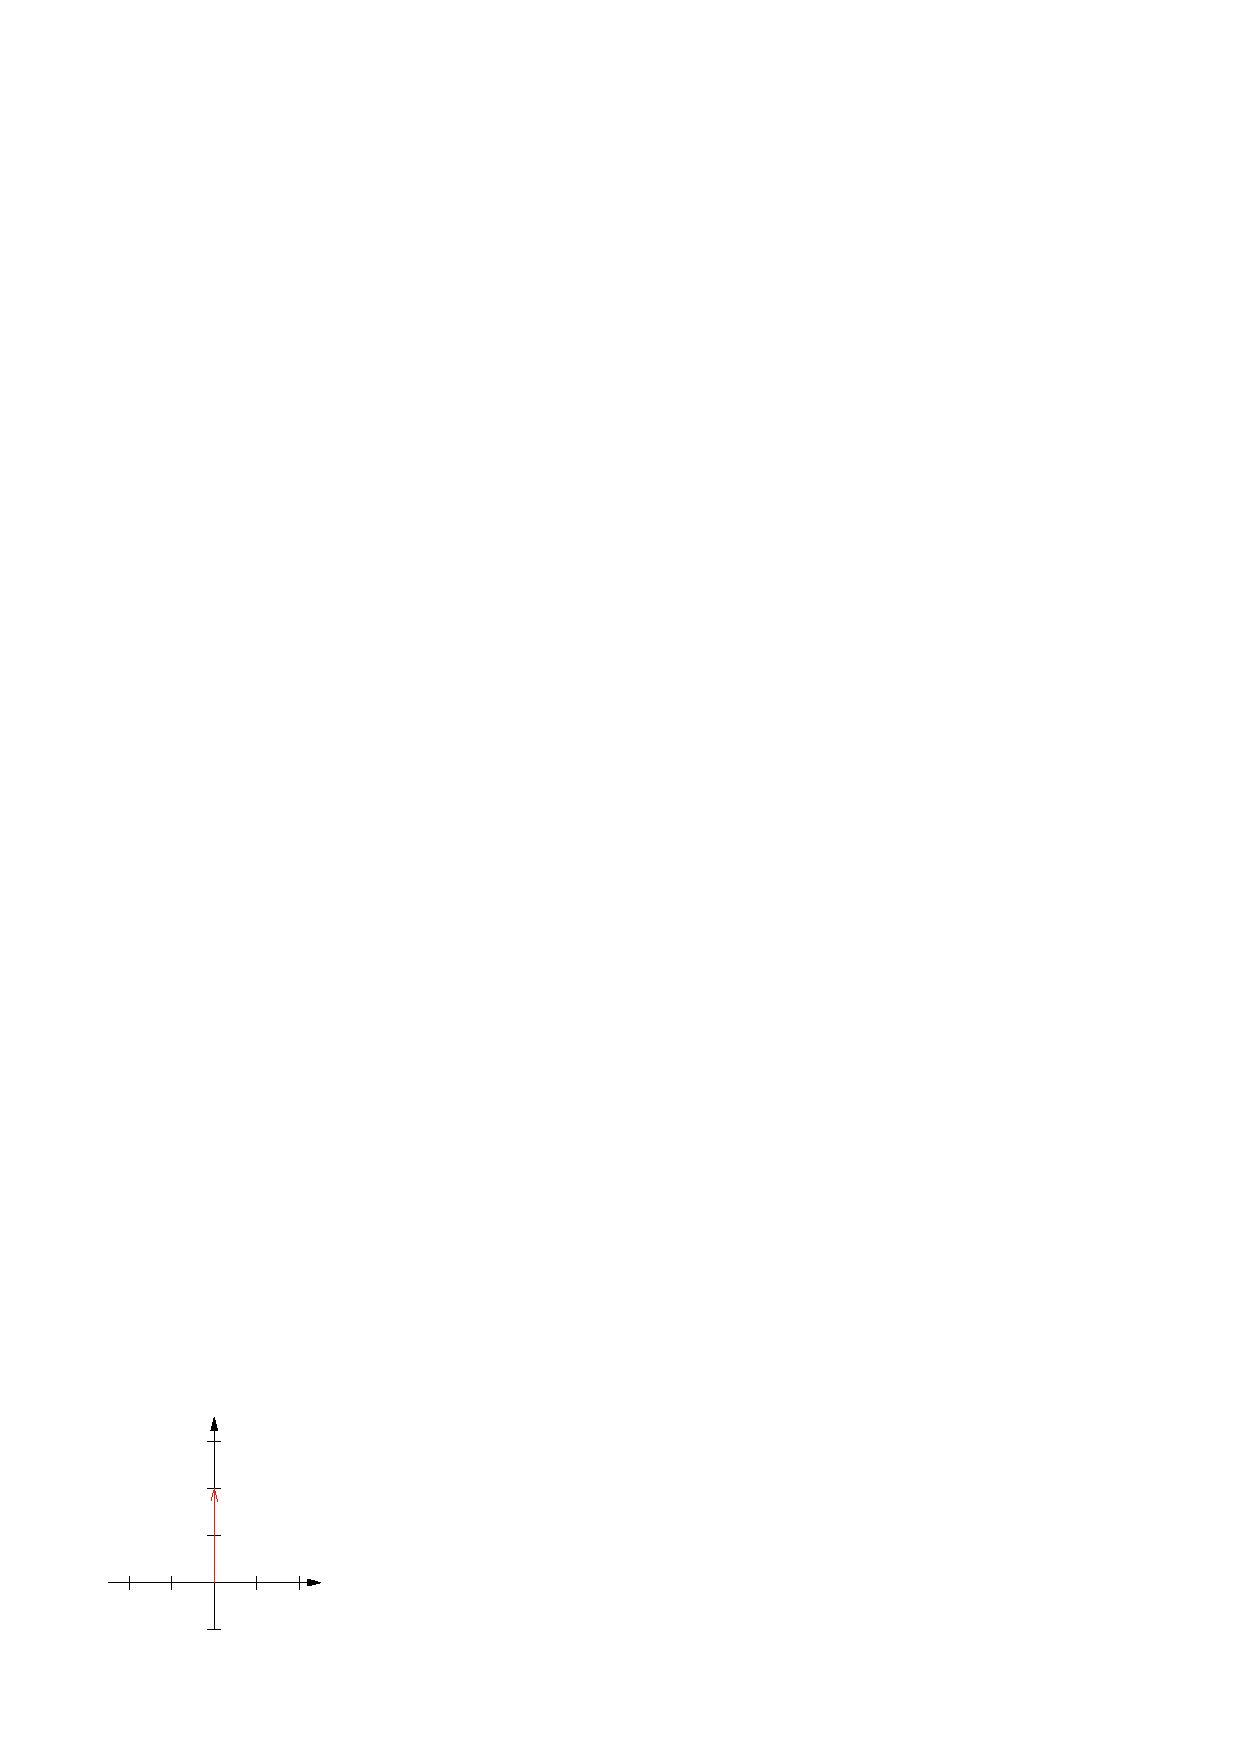
\includegraphics[width={108.00bp},height={108.00bp}]{figura_03_12}}%
    \gplfronttext
  \end{picture}%
\endgroup

\end{figure}
\begin{equation*}
    \delta(t)=\begin{cases}
        0&t\neq0\\
        \infty&t=0\\
    \end{cases}
\end{equation*}

Tal que:
\begin{equation*}
    \int_{-\xi}^{\xi}\delta(t)\,dt=1
\end{equation*}

Por tanto:
\begin{equation}
    k\delta(t)=\begin{cases}
        0&t\neq0\\
        \pm\infty&t=0\\
    \end{cases}
\end{equation}
\begin{figure}[H]
    \centering
    \begin{minipage}{.4\textwidth}
        \centering
        % GNUPLOT: LaTeX picture with Postscript
\begingroup
  \makeatletter
  \providecommand\color[2][]{%
    \GenericError{(gnuplot) \space\space\space\@spaces}{%
      Package color not loaded in conjunction with
      terminal option `colourtext'%
    }{See the gnuplot documentation for explanation.%
    }{Either use 'blacktext' in gnuplot or load the package
      color.sty in LaTeX.}%
    \renewcommand\color[2][]{}%
  }%
  \providecommand\includegraphics[2][]{%
    \GenericError{(gnuplot) \space\space\space\@spaces}{%
      Package graphicx or graphics not loaded%
    }{See the gnuplot documentation for explanation.%
    }{The gnuplot epslatex terminal needs graphicx.sty or graphics.sty.}%
    \renewcommand\includegraphics[2][]{}%
  }%
  \providecommand\rotatebox[2]{#2}%
  \@ifundefined{ifGPcolor}{%
    \newif\ifGPcolor
    \GPcolorfalse
  }{}%
  \@ifundefined{ifGPblacktext}{%
    \newif\ifGPblacktext
    \GPblacktexttrue
  }{}%
  % define a \g@addto@macro without @ in the name:
  \let\gplgaddtomacro\g@addto@macro
  % define empty templates for all commands taking text:
  \gdef\gplbacktext{}%
  \gdef\gplfronttext{}%
  \makeatother
  \ifGPblacktext
    % no textcolor at all
    \def\colorrgb#1{}%
    \def\colorgray#1{}%
  \else
    % gray or color?
    \ifGPcolor
      \def\colorrgb#1{\color[rgb]{#1}}%
      \def\colorgray#1{\color[gray]{#1}}%
      \expandafter\def\csname LTw\endcsname{\color{white}}%
      \expandafter\def\csname LTb\endcsname{\color{black}}%
      \expandafter\def\csname LTa\endcsname{\color{black}}%
      \expandafter\def\csname LT0\endcsname{\color[rgb]{1,0,0}}%
      \expandafter\def\csname LT1\endcsname{\color[rgb]{0,1,0}}%
      \expandafter\def\csname LT2\endcsname{\color[rgb]{0,0,1}}%
      \expandafter\def\csname LT3\endcsname{\color[rgb]{1,0,1}}%
      \expandafter\def\csname LT4\endcsname{\color[rgb]{0,1,1}}%
      \expandafter\def\csname LT5\endcsname{\color[rgb]{1,1,0}}%
      \expandafter\def\csname LT6\endcsname{\color[rgb]{0,0,0}}%
      \expandafter\def\csname LT7\endcsname{\color[rgb]{1,0.3,0}}%
      \expandafter\def\csname LT8\endcsname{\color[rgb]{0.5,0.5,0.5}}%
    \else
      % gray
      \def\colorrgb#1{\color{black}}%
      \def\colorgray#1{\color[gray]{#1}}%
      \expandafter\def\csname LTw\endcsname{\color{white}}%
      \expandafter\def\csname LTb\endcsname{\color{black}}%
      \expandafter\def\csname LTa\endcsname{\color{black}}%
      \expandafter\def\csname LT0\endcsname{\color{black}}%
      \expandafter\def\csname LT1\endcsname{\color{black}}%
      \expandafter\def\csname LT2\endcsname{\color{black}}%
      \expandafter\def\csname LT3\endcsname{\color{black}}%
      \expandafter\def\csname LT4\endcsname{\color{black}}%
      \expandafter\def\csname LT5\endcsname{\color{black}}%
      \expandafter\def\csname LT6\endcsname{\color{black}}%
      \expandafter\def\csname LT7\endcsname{\color{black}}%
      \expandafter\def\csname LT8\endcsname{\color{black}}%
    \fi
  \fi
    \setlength{\unitlength}{0.0500bp}%
    \ifx\gptboxheight\undefined%
      \newlength{\gptboxheight}%
      \newlength{\gptboxwidth}%
      \newsavebox{\gptboxtext}%
    \fi%
    \setlength{\fboxrule}{0.5pt}%
    \setlength{\fboxsep}{1pt}%
    \definecolor{tbcol}{rgb}{1,1,1}%
\begin{picture}(2160.00,2160.00)%
    \gplgaddtomacro\gplbacktext{%
      \csname LTb\endcsname%%
      \put(960,192){\makebox(0,0)[r]{\strut{}}}%
      \put(960,644){\makebox(0,0)[r]{\strut{}}}%
      \put(960,1096){\makebox(0,0)[r]{\strut{}}}%
      \put(960,1547){\makebox(0,0)[r]{\strut{}}}%
      \put(960,1999){\makebox(0,0)[r]{\strut{}}}%
      \put(240,421){\makebox(0,0){\strut{}}}%
      \put(648,421){\makebox(0,0){\strut{}}}%
      \put(1056,421){\makebox(0,0){\strut{}}}%
      \put(1463,421){\makebox(0,0){\strut{}}}%
      \put(1871,421){\makebox(0,0){\strut{}}}%
      \csname LTb\endcsname%%
      \put(2279,644){\makebox(0,0)[l]{\strut{}$t$}}%
      \put(1239,2180){\makebox(0,0)[l]{\strut{}$f(t)$}}%
      \put(1626,1547){\makebox(0,0)[l]{\strut{}$k\delta(t-t_0)$}}%
      \put(1626,1276){\makebox(0,0)[l]{\strut{}$k>0$}}%
      \put(1422,463){\makebox(0,0)[l]{\strut{}$t_0$}}%
    }%
    \gplgaddtomacro\gplfronttext{%
    }%
    \gplbacktext
    \put(0,0){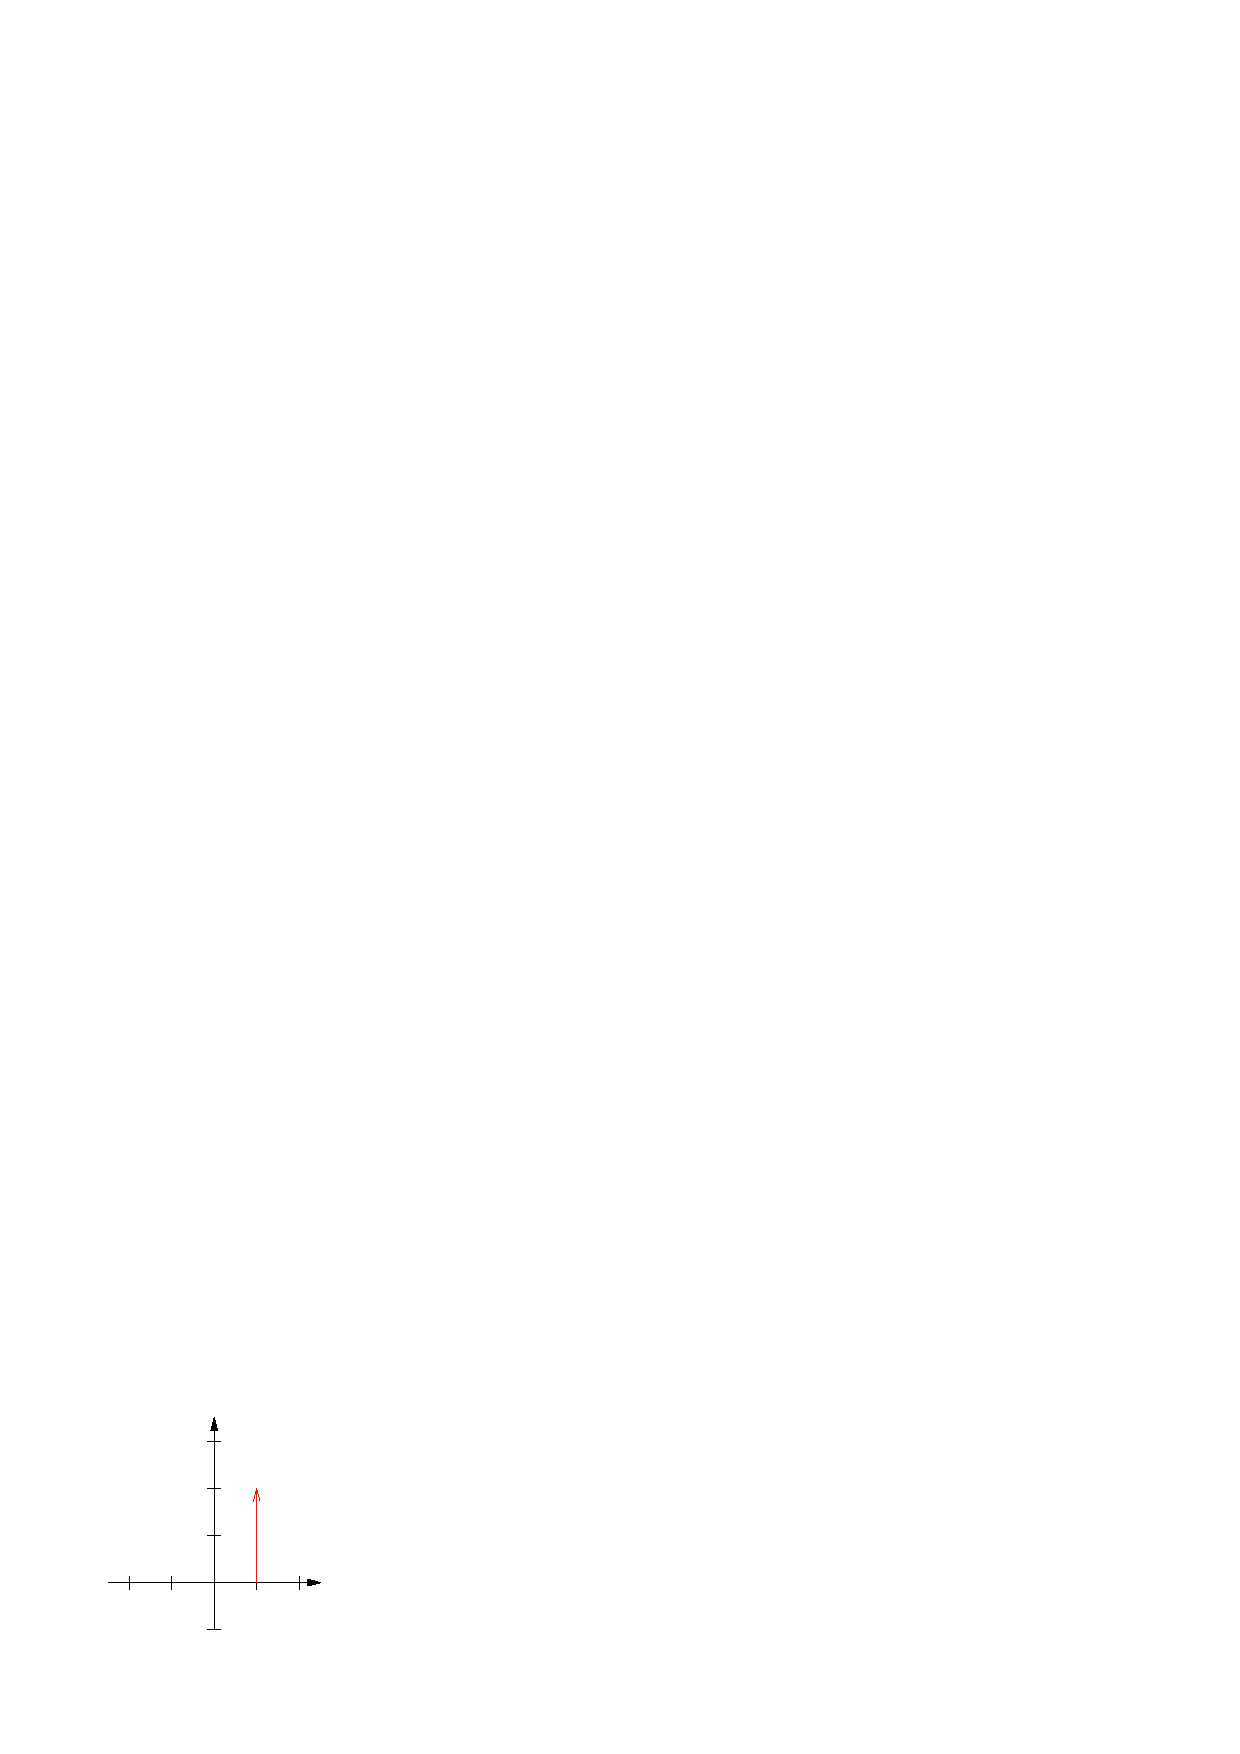
\includegraphics[width={108.00bp},height={108.00bp}]{figura_03_13}}%
    \gplfronttext
  \end{picture}%
\endgroup

    \end{minipage}
    \begin{minipage}{.4\textwidth}
        \centering
        % GNUPLOT: LaTeX picture with Postscript
\begingroup
  \makeatletter
  \providecommand\color[2][]{%
    \GenericError{(gnuplot) \space\space\space\@spaces}{%
      Package color not loaded in conjunction with
      terminal option `colourtext'%
    }{See the gnuplot documentation for explanation.%
    }{Either use 'blacktext' in gnuplot or load the package
      color.sty in LaTeX.}%
    \renewcommand\color[2][]{}%
  }%
  \providecommand\includegraphics[2][]{%
    \GenericError{(gnuplot) \space\space\space\@spaces}{%
      Package graphicx or graphics not loaded%
    }{See the gnuplot documentation for explanation.%
    }{The gnuplot epslatex terminal needs graphicx.sty or graphics.sty.}%
    \renewcommand\includegraphics[2][]{}%
  }%
  \providecommand\rotatebox[2]{#2}%
  \@ifundefined{ifGPcolor}{%
    \newif\ifGPcolor
    \GPcolorfalse
  }{}%
  \@ifundefined{ifGPblacktext}{%
    \newif\ifGPblacktext
    \GPblacktexttrue
  }{}%
  % define a \g@addto@macro without @ in the name:
  \let\gplgaddtomacro\g@addto@macro
  % define empty templates for all commands taking text:
  \gdef\gplbacktext{}%
  \gdef\gplfronttext{}%
  \makeatother
  \ifGPblacktext
    % no textcolor at all
    \def\colorrgb#1{}%
    \def\colorgray#1{}%
  \else
    % gray or color?
    \ifGPcolor
      \def\colorrgb#1{\color[rgb]{#1}}%
      \def\colorgray#1{\color[gray]{#1}}%
      \expandafter\def\csname LTw\endcsname{\color{white}}%
      \expandafter\def\csname LTb\endcsname{\color{black}}%
      \expandafter\def\csname LTa\endcsname{\color{black}}%
      \expandafter\def\csname LT0\endcsname{\color[rgb]{1,0,0}}%
      \expandafter\def\csname LT1\endcsname{\color[rgb]{0,1,0}}%
      \expandafter\def\csname LT2\endcsname{\color[rgb]{0,0,1}}%
      \expandafter\def\csname LT3\endcsname{\color[rgb]{1,0,1}}%
      \expandafter\def\csname LT4\endcsname{\color[rgb]{0,1,1}}%
      \expandafter\def\csname LT5\endcsname{\color[rgb]{1,1,0}}%
      \expandafter\def\csname LT6\endcsname{\color[rgb]{0,0,0}}%
      \expandafter\def\csname LT7\endcsname{\color[rgb]{1,0.3,0}}%
      \expandafter\def\csname LT8\endcsname{\color[rgb]{0.5,0.5,0.5}}%
    \else
      % gray
      \def\colorrgb#1{\color{black}}%
      \def\colorgray#1{\color[gray]{#1}}%
      \expandafter\def\csname LTw\endcsname{\color{white}}%
      \expandafter\def\csname LTb\endcsname{\color{black}}%
      \expandafter\def\csname LTa\endcsname{\color{black}}%
      \expandafter\def\csname LT0\endcsname{\color{black}}%
      \expandafter\def\csname LT1\endcsname{\color{black}}%
      \expandafter\def\csname LT2\endcsname{\color{black}}%
      \expandafter\def\csname LT3\endcsname{\color{black}}%
      \expandafter\def\csname LT4\endcsname{\color{black}}%
      \expandafter\def\csname LT5\endcsname{\color{black}}%
      \expandafter\def\csname LT6\endcsname{\color{black}}%
      \expandafter\def\csname LT7\endcsname{\color{black}}%
      \expandafter\def\csname LT8\endcsname{\color{black}}%
    \fi
  \fi
    \setlength{\unitlength}{0.0500bp}%
    \ifx\gptboxheight\undefined%
      \newlength{\gptboxheight}%
      \newlength{\gptboxwidth}%
      \newsavebox{\gptboxtext}%
    \fi%
    \setlength{\fboxrule}{0.5pt}%
    \setlength{\fboxsep}{1pt}%
    \definecolor{tbcol}{rgb}{1,1,1}%
\begin{picture}(2160.00,2160.00)%
    \gplgaddtomacro\gplbacktext{%
      \csname LTb\endcsname%%
      \put(960,192){\makebox(0,0)[r]{\strut{}}}%
      \put(960,644){\makebox(0,0)[r]{\strut{}}}%
      \put(960,1096){\makebox(0,0)[r]{\strut{}}}%
      \put(960,1547){\makebox(0,0)[r]{\strut{}}}%
      \put(960,1999){\makebox(0,0)[r]{\strut{}}}%
      \put(240,1324){\makebox(0,0){\strut{}}}%
      \put(648,1324){\makebox(0,0){\strut{}}}%
      \put(1056,1324){\makebox(0,0){\strut{}}}%
      \put(1463,1324){\makebox(0,0){\strut{}}}%
      \put(1871,1324){\makebox(0,0){\strut{}}}%
      \csname LTb\endcsname%%
      \put(2279,1547){\makebox(0,0)[l]{\strut{}$t$}}%
      \put(1239,2180){\makebox(0,0)[l]{\strut{}$f(t)$}}%
      \put(1626,644){\makebox(0,0)[l]{\strut{}$k\delta(t-t_0)$}}%
      \put(1626,915){\makebox(0,0)[l]{\strut{}$k<0$}}%
      \put(1422,1728){\makebox(0,0)[l]{\strut{}$t_0$}}%
    }%
    \gplgaddtomacro\gplfronttext{%
    }%
    \gplbacktext
    \put(0,0){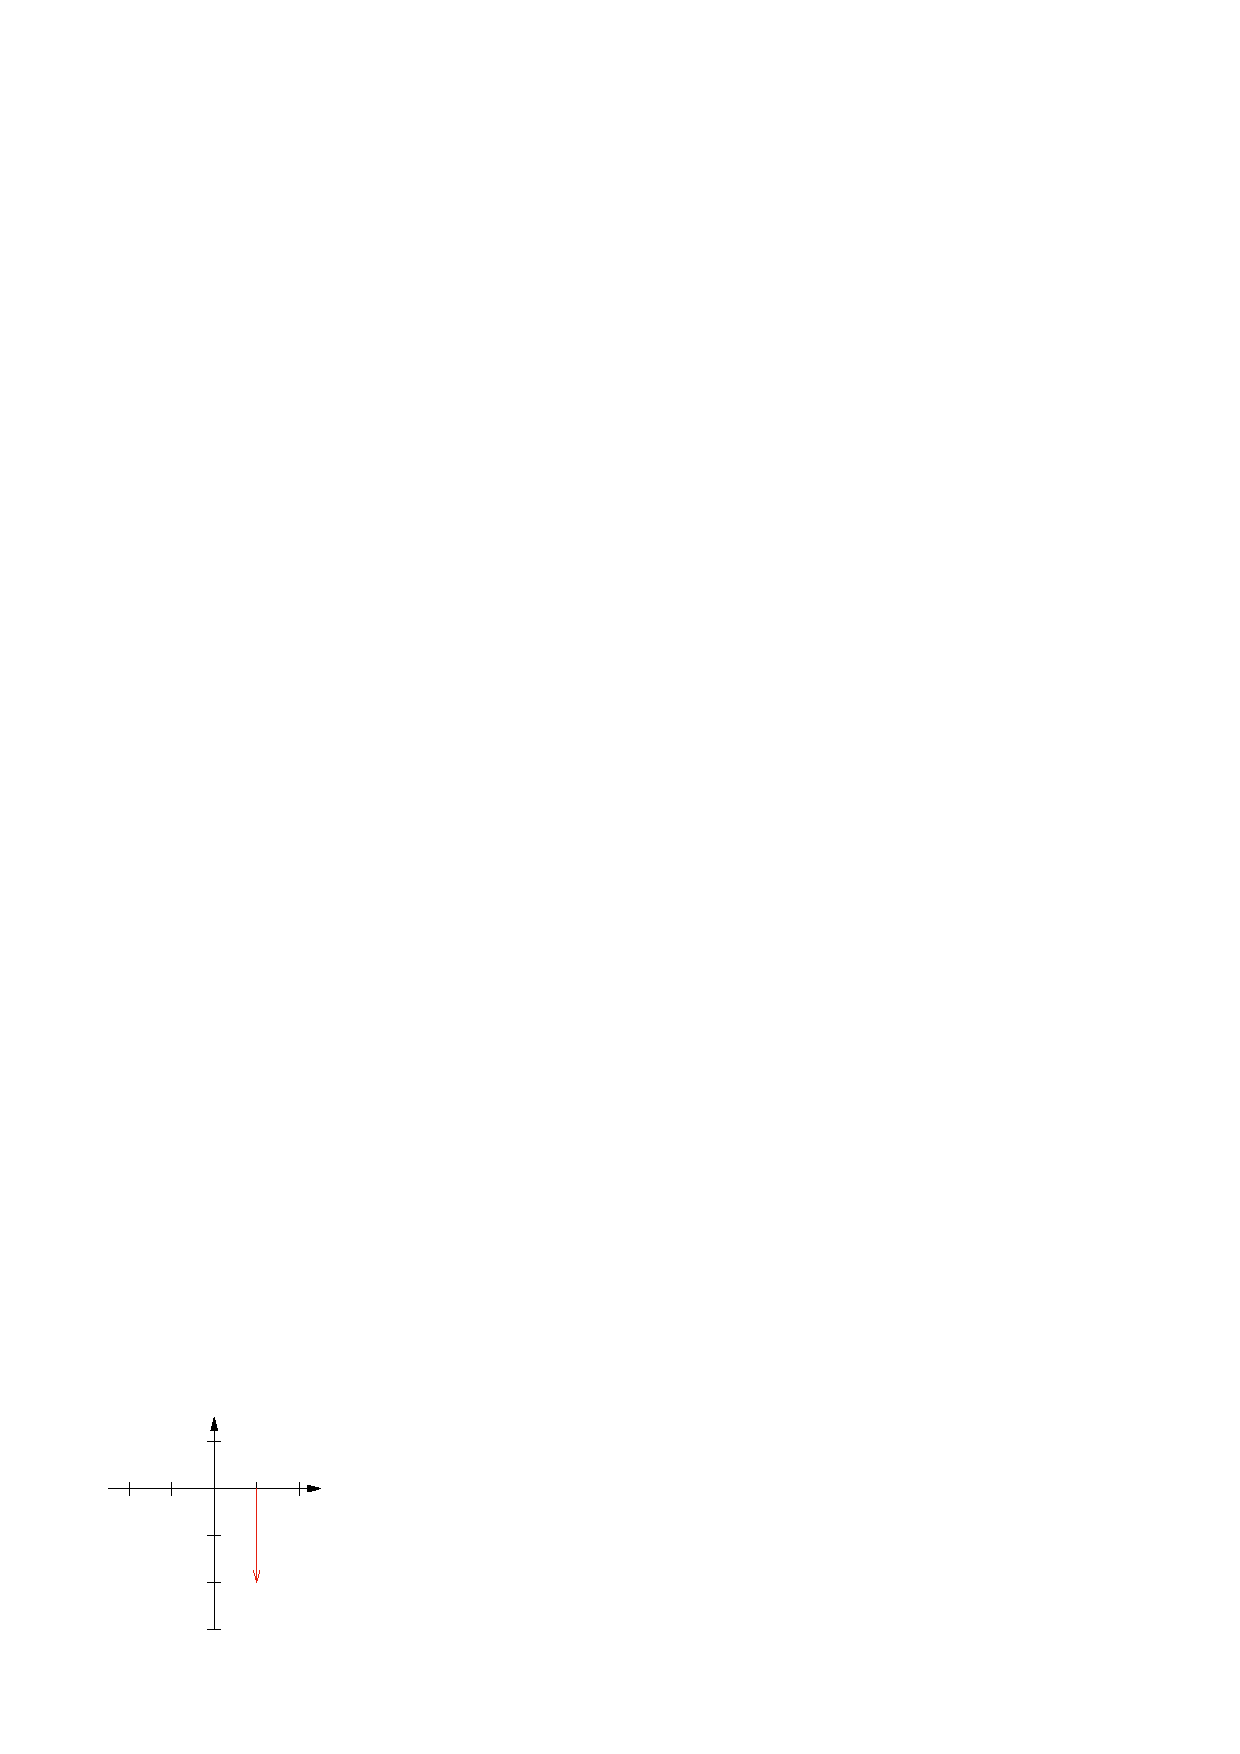
\includegraphics[width={108.00bp},height={108.00bp}]{figura_03_14}}%
    \gplfronttext
  \end{picture}%
\endgroup

    \end{minipage}
\end{figure}

Si: $\phi(t)$ es una función de prueba:
\begin{equation}
    \phi(t)\delta(t-t_0)=\phi(t_0)\delta(t-t_0)
\end{equation}
\begin{figure}[H]
    \centering
    % GNUPLOT: LaTeX picture with Postscript
\begingroup
  \makeatletter
  \providecommand\color[2][]{%
    \GenericError{(gnuplot) \space\space\space\@spaces}{%
      Package color not loaded in conjunction with
      terminal option `colourtext'%
    }{See the gnuplot documentation for explanation.%
    }{Either use 'blacktext' in gnuplot or load the package
      color.sty in LaTeX.}%
    \renewcommand\color[2][]{}%
  }%
  \providecommand\includegraphics[2][]{%
    \GenericError{(gnuplot) \space\space\space\@spaces}{%
      Package graphicx or graphics not loaded%
    }{See the gnuplot documentation for explanation.%
    }{The gnuplot epslatex terminal needs graphicx.sty or graphics.sty.}%
    \renewcommand\includegraphics[2][]{}%
  }%
  \providecommand\rotatebox[2]{#2}%
  \@ifundefined{ifGPcolor}{%
    \newif\ifGPcolor
    \GPcolorfalse
  }{}%
  \@ifundefined{ifGPblacktext}{%
    \newif\ifGPblacktext
    \GPblacktexttrue
  }{}%
  % define a \g@addto@macro without @ in the name:
  \let\gplgaddtomacro\g@addto@macro
  % define empty templates for all commands taking text:
  \gdef\gplbacktext{}%
  \gdef\gplfronttext{}%
  \makeatother
  \ifGPblacktext
    % no textcolor at all
    \def\colorrgb#1{}%
    \def\colorgray#1{}%
  \else
    % gray or color?
    \ifGPcolor
      \def\colorrgb#1{\color[rgb]{#1}}%
      \def\colorgray#1{\color[gray]{#1}}%
      \expandafter\def\csname LTw\endcsname{\color{white}}%
      \expandafter\def\csname LTb\endcsname{\color{black}}%
      \expandafter\def\csname LTa\endcsname{\color{black}}%
      \expandafter\def\csname LT0\endcsname{\color[rgb]{1,0,0}}%
      \expandafter\def\csname LT1\endcsname{\color[rgb]{0,1,0}}%
      \expandafter\def\csname LT2\endcsname{\color[rgb]{0,0,1}}%
      \expandafter\def\csname LT3\endcsname{\color[rgb]{1,0,1}}%
      \expandafter\def\csname LT4\endcsname{\color[rgb]{0,1,1}}%
      \expandafter\def\csname LT5\endcsname{\color[rgb]{1,1,0}}%
      \expandafter\def\csname LT6\endcsname{\color[rgb]{0,0,0}}%
      \expandafter\def\csname LT7\endcsname{\color[rgb]{1,0.3,0}}%
      \expandafter\def\csname LT8\endcsname{\color[rgb]{0.5,0.5,0.5}}%
    \else
      % gray
      \def\colorrgb#1{\color{black}}%
      \def\colorgray#1{\color[gray]{#1}}%
      \expandafter\def\csname LTw\endcsname{\color{white}}%
      \expandafter\def\csname LTb\endcsname{\color{black}}%
      \expandafter\def\csname LTa\endcsname{\color{black}}%
      \expandafter\def\csname LT0\endcsname{\color{black}}%
      \expandafter\def\csname LT1\endcsname{\color{black}}%
      \expandafter\def\csname LT2\endcsname{\color{black}}%
      \expandafter\def\csname LT3\endcsname{\color{black}}%
      \expandafter\def\csname LT4\endcsname{\color{black}}%
      \expandafter\def\csname LT5\endcsname{\color{black}}%
      \expandafter\def\csname LT6\endcsname{\color{black}}%
      \expandafter\def\csname LT7\endcsname{\color{black}}%
      \expandafter\def\csname LT8\endcsname{\color{black}}%
    \fi
  \fi
    \setlength{\unitlength}{0.0500bp}%
    \ifx\gptboxheight\undefined%
      \newlength{\gptboxheight}%
      \newlength{\gptboxwidth}%
      \newsavebox{\gptboxtext}%
    \fi%
    \setlength{\fboxrule}{0.5pt}%
    \setlength{\fboxsep}{1pt}%
    \definecolor{tbcol}{rgb}{1,1,1}%
\begin{picture}(4320.00,2880.00)%
    \gplgaddtomacro\gplbacktext{%
      \csname LTb\endcsname%%
      \put(2040,192){\makebox(0,0)[r]{\strut{}}}%
      \put(2040,553){\makebox(0,0)[r]{\strut{}}}%
      \put(2040,914){\makebox(0,0)[r]{\strut{}}}%
      \put(2040,1275){\makebox(0,0)[r]{\strut{}}}%
      \put(2040,1636){\makebox(0,0)[r]{\strut{}}}%
      \put(2040,1997){\makebox(0,0)[r]{\strut{}}}%
      \put(2040,2358){\makebox(0,0)[r]{\strut{}}}%
      \put(2040,2719){\makebox(0,0)[r]{\strut{}}}%
      \put(240,330){\makebox(0,0){\strut{}}}%
      \put(714,330){\makebox(0,0){\strut{}}}%
      \put(1188,330){\makebox(0,0){\strut{}}}%
      \put(1662,330){\makebox(0,0){\strut{}}}%
      \put(2136,330){\makebox(0,0){\strut{}}}%
      \put(2609,330){\makebox(0,0){\strut{}}}%
      \put(3083,330){\makebox(0,0){\strut{}}}%
      \put(3557,330){\makebox(0,0){\strut{}}}%
      \put(4031,330){\makebox(0,0){\strut{}}}%
      \csname LTb\endcsname%%
      \put(4647,553){\makebox(0,0)[l]{\strut{}$t$}}%
      \put(2349,2863){\makebox(0,0)[l]{\strut{}$f(t)$}}%
      \put(2562,336){\makebox(0,0)[l]{\strut{}$t_0$}}%
      \put(1235,1275){\makebox(0,0)[l]{\strut{}$\phi(t_0)$}}%
      \put(714,2178){\makebox(0,0)[l]{\strut{}$\phi(t)$}}%
      \put(2799,2178){\makebox(0,0)[l]{\strut{}$\delta(t-t_0)$}}%
    }%
    \gplgaddtomacro\gplfronttext{%
    }%
    \gplbacktext
    \put(0,0){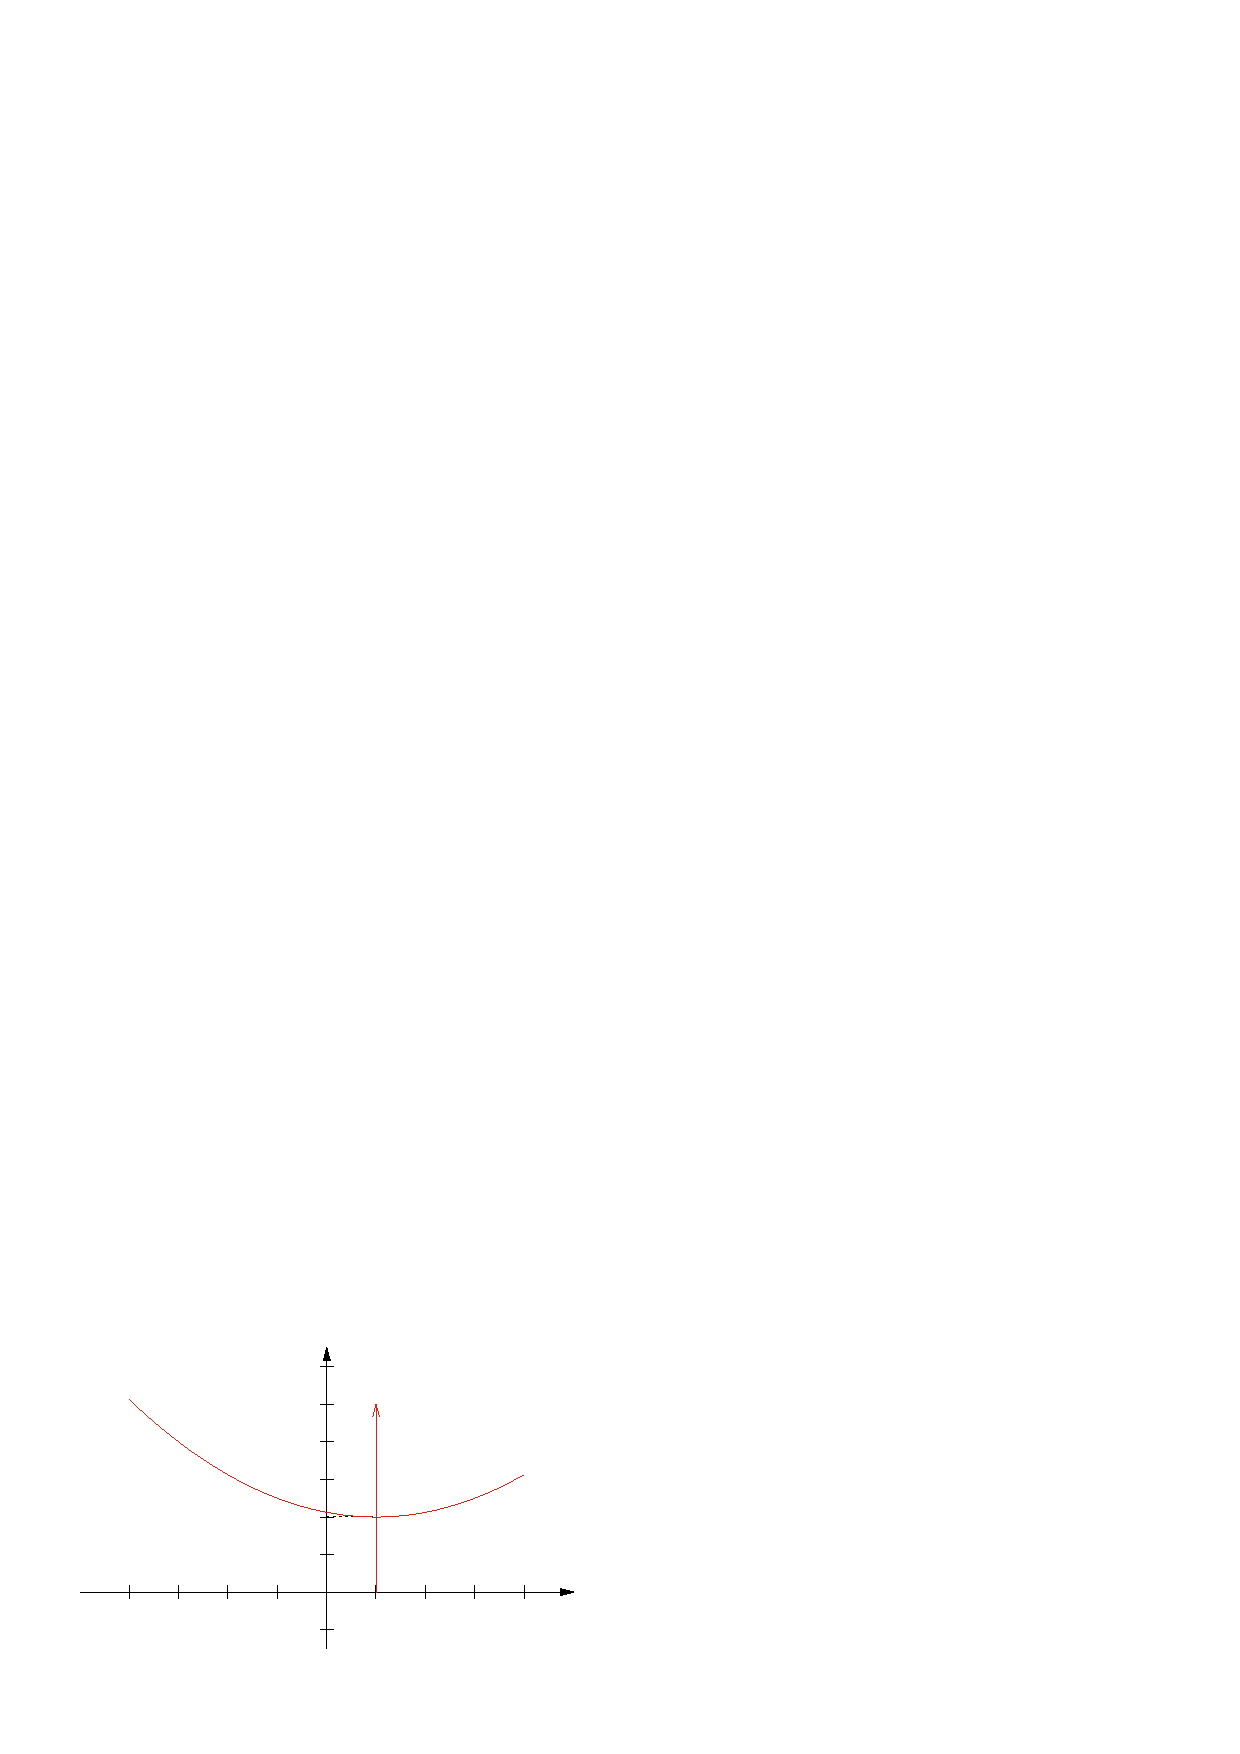
\includegraphics[width={216.00bp},height={144.00bp}]{figura_03_15}}%
    \gplfronttext
  \end{picture}%
\endgroup

\end{figure}

Para $t\neq0$
\begin{equation*}
    \phi(t)\delta(t-t_0)=0
\end{equation*}

Para $t=0$
\begin{equation*}
    \phi(t)\delta(t-t_0)=\phi(t_0)\delta(t-t_0)
\end{equation*}

\subsection{Propiedades de la función impulso}
\subsubsection*{Propiedad 1}
\begin{equation*}
    \int_a^b\delta(t-t_0)\,dt=\begin{cases}
        1&t_0\in[a,b]\\
        0&t_0\notin[a,b]\\
    \end{cases}
\end{equation*}

En general:
\begin{equation}
    \int_{-\infty}^{\infty}\delta(t-t_0)\,dt=1
\end{equation}

\subsubsection*{Propiedad 2}
\begin{equation*}
    \int_a^b\phi(t)\,\delta(t-t_0)\,dt=\begin{cases}
        \phi(t_0)&t_0\in[a,b]\\
        0&t_0\notin[a,b]\\
    \end{cases}
\end{equation*}

En general:
\begin{equation}
    \int_{-\infty}^{\infty}\phi(t_0)\,\delta(t-t_0)\,dt=\phi(t_0)
\end{equation}

\underline{Prueba}:
\begin{equation*}
\begin{split}
    \int_{-\infty}^{\infty}\phi(t)\delta(t-t_0)\,dt
        &=\int_{-\infty}^{\infty}\phi(t_0)\delta(t-t_0)\,dt\\
        &=\phi(t_0)\int_{-\infty}^{\infty}\delta(t-t_0)\,dt\\
        &=\phi(t_0)\\
\end{split}
\end{equation*}

\subsubsection*{Propiedad 3}
\begin{equation}
    \int_{-\infty}^{\infty}\phi(t)\,\delta(at)\,dt
        =\frac{1}{|a|}\int_{-\infty}^{\infty}
            \phi\left(\frac{t}{a}\right)\delta(t)\,dt
        =\frac{\phi(0)}{|a|};a\neq0
\end{equation}

\underline{Prueba}:

Realizando un cambio de variable:
\begin{equation*}
    \tau=at
\end{equation*}
\begin{equation*}
    d\tau=a\,dt
\end{equation*}

Para $a>0$:
\begin{equation*}
    \int_{-\infty}^{\infty}
        \phi\left(\frac{\tau}{a}\right)\delta(\tau)\,\frac{d\tau}{a}
        =\frac{1}{a}\int_{-\infty}^{\infty}
            \phi\left(\frac{\tau}{a}\right)\delta(\tau)d\tau
\end{equation*}

Para $a<0$:
\begin{equation*}
    \int_{-\infty}^{\infty}
        \phi\left(\frac{\tau}{a}\right)\delta(\tau)\,\frac{d\tau}{a}
        =-\frac{1}{a}\int_{-\infty}^{\infty}
            \phi\left(\frac{\tau}{a}\right)\delta(\tau)d\tau
\end{equation*}

Como:
\begin{equation*}
    |a|=\begin{cases}
        -a&a<0\\
        a&a>0\\
    \end{cases}
\end{equation*}
\begin{equation*}
\begin{split}
    \int_{-\infty}^{\infty}\phi(t)\,\delta(at)\,dt
        &=\frac{1}{|a|}\int_{-\infty}^{\infty}
            \phi\left(\frac{\tau}{a}\right)\delta(\tau)\,d\tau\\
        &=\frac{1}{|a|}\phi\left(\frac{0}{a}\right)\\
        &=\frac{\phi(0)}{|a|}\\
\end{split}
\end{equation*}

\subsubsection*{Propiedad 4}
\begin{equation}
    \delta(at)=\frac{1}{|a|}\delta(t)
\end{equation}

En particular:
\begin{equation}
    \delta(-t)=\delta(t)
\end{equation}

Por tanto $\delta(t)$ es una función \textbf{par}.

\underline{Prueba}:
\begin{equation*}
\begin{split}
    \int_{-\infty}^{\infty}\phi(t)\,\delta(at)\,dt
        &=\frac{1}{|a|}\phi(0)\\
        &=\frac{1}{|a|}\int_{-\infty}^{\infty}\phi(t)\,\delta(t)\,dt\\
\end{split}
\end{equation*}
\begin{equation*}
    \phi(t)\,\delta(at)=\frac{1}{|a|}\phi(t)\,\delta(t)
\end{equation*}
\begin{equation*}
    \delta(at)=\frac{1}{|a|}\,\delta(t)
\end{equation*}

Para $a=-1$:
\begin{equation*}
    \delta(-t)=\frac{1}{|-1|}\,\delta(t)=\delta(t)
\end{equation*}

\subsubsection*{Propiedad 5}
\begin{equation*}
    t\,\delta(t)=0
\end{equation*}
\begin{equation}
    t^n\,\delta(t)=0;n\in\mathbb{N}
\end{equation}

\underline{Prueba}:

\begin{equation*}
    \int_{-\infty}^{\infty}t^n\,\delta(t)\,dt=0^n=0
\end{equation*}

Derivando ambos miembros:
\begin{equation*}
    t^n\,\delta(t)\,dt=0
\end{equation*}

\section{Derivada de la función impulso}
\begin{equation*}
    \delta'(t)=\frac{d}{dt}(\delta(t))
\end{equation*}
\begin{equation}
    \int_{-\infty}^{\infty}\phi(t)\delta'(t)\,dt
        =-\int_{-\infty}^{\infty}\phi'(t)\delta(t)\,dt
        =-\phi'(0)
\end{equation}

\underline{Prueba}:

Realizando la integración por partes:
\begin{equation*}
    u=\phi(t)
\end{equation*}
\begin{equation*}
    du=\phi'(t)\,dt
\end{equation*}
\begin{equation*}
    dv=\delta'(t-t_0)\,dt
\end{equation*}
\begin{equation*}
    v=\delta(t-t_0)
\end{equation*}
\begin{equation*}
\begin{split}
    \int_{-\infty}^{\infty}\phi(t)\delta'(t-t_0)\,dt
        &=(\phi(t)\delta(t-t_0)\Big|_{-\infty}^{\infty})
        -\int_{-\infty}^{\infty}\delta(t-t_0)\phi'(t)\,dt\\
        &=0-\int_{-\infty}^{\infty}\delta(t-t_0)\phi'(t)\,dt\\
        &=-\phi'(t_0)
\end{split}
\end{equation*}

\subsubsection{Derivadas de orden superior}
\begin{equation*}
\begin{split}
    \int_{-\infty}^{\infty}\phi(t)\delta''(t)\,dt
        &=\int_{-\infty}^{\infty}\phi(t)(\delta'(t))'\,dt\\
        &=-\int_{-\infty}^{\infty}\phi'(t)\delta'(t)\,dt\\
        &=\int_{-\infty}^{\infty}\phi''(t)\delta(t)\,dt\\
        &=\phi''(0)\\
\end{split}
\end{equation*}

De igual manera:
\begin{equation*}
    \int_{-\infty}^{\infty}\phi(t)\delta^{\prime\prime\prime}(t-t_0)\,dt
        =-\phi^{\prime\prime\prime}(t_0)
\end{equation*}

En general:
\begin{equation}
    \int_{-\infty}^{\infty}\phi(t)\delta^{(n)}(t-t_0)\,dt
        ={(-1)}^n\phi^{(n)}(t_0)
\end{equation}

\section{Derivada de la función escalón unitario}
\begin{figure}[H]
    \centering
    \begin{minipage}{.4\textwidth}
        \centering
        % GNUPLOT: LaTeX picture with Postscript
\begingroup
  \makeatletter
  \providecommand\color[2][]{%
    \GenericError{(gnuplot) \space\space\space\@spaces}{%
      Package color not loaded in conjunction with
      terminal option `colourtext'%
    }{See the gnuplot documentation for explanation.%
    }{Either use 'blacktext' in gnuplot or load the package
      color.sty in LaTeX.}%
    \renewcommand\color[2][]{}%
  }%
  \providecommand\includegraphics[2][]{%
    \GenericError{(gnuplot) \space\space\space\@spaces}{%
      Package graphicx or graphics not loaded%
    }{See the gnuplot documentation for explanation.%
    }{The gnuplot epslatex terminal needs graphicx.sty or graphics.sty.}%
    \renewcommand\includegraphics[2][]{}%
  }%
  \providecommand\rotatebox[2]{#2}%
  \@ifundefined{ifGPcolor}{%
    \newif\ifGPcolor
    \GPcolorfalse
  }{}%
  \@ifundefined{ifGPblacktext}{%
    \newif\ifGPblacktext
    \GPblacktexttrue
  }{}%
  % define a \g@addto@macro without @ in the name:
  \let\gplgaddtomacro\g@addto@macro
  % define empty templates for all commands taking text:
  \gdef\gplbacktext{}%
  \gdef\gplfronttext{}%
  \makeatother
  \ifGPblacktext
    % no textcolor at all
    \def\colorrgb#1{}%
    \def\colorgray#1{}%
  \else
    % gray or color?
    \ifGPcolor
      \def\colorrgb#1{\color[rgb]{#1}}%
      \def\colorgray#1{\color[gray]{#1}}%
      \expandafter\def\csname LTw\endcsname{\color{white}}%
      \expandafter\def\csname LTb\endcsname{\color{black}}%
      \expandafter\def\csname LTa\endcsname{\color{black}}%
      \expandafter\def\csname LT0\endcsname{\color[rgb]{1,0,0}}%
      \expandafter\def\csname LT1\endcsname{\color[rgb]{0,1,0}}%
      \expandafter\def\csname LT2\endcsname{\color[rgb]{0,0,1}}%
      \expandafter\def\csname LT3\endcsname{\color[rgb]{1,0,1}}%
      \expandafter\def\csname LT4\endcsname{\color[rgb]{0,1,1}}%
      \expandafter\def\csname LT5\endcsname{\color[rgb]{1,1,0}}%
      \expandafter\def\csname LT6\endcsname{\color[rgb]{0,0,0}}%
      \expandafter\def\csname LT7\endcsname{\color[rgb]{1,0.3,0}}%
      \expandafter\def\csname LT8\endcsname{\color[rgb]{0.5,0.5,0.5}}%
    \else
      % gray
      \def\colorrgb#1{\color{black}}%
      \def\colorgray#1{\color[gray]{#1}}%
      \expandafter\def\csname LTw\endcsname{\color{white}}%
      \expandafter\def\csname LTb\endcsname{\color{black}}%
      \expandafter\def\csname LTa\endcsname{\color{black}}%
      \expandafter\def\csname LT0\endcsname{\color{black}}%
      \expandafter\def\csname LT1\endcsname{\color{black}}%
      \expandafter\def\csname LT2\endcsname{\color{black}}%
      \expandafter\def\csname LT3\endcsname{\color{black}}%
      \expandafter\def\csname LT4\endcsname{\color{black}}%
      \expandafter\def\csname LT5\endcsname{\color{black}}%
      \expandafter\def\csname LT6\endcsname{\color{black}}%
      \expandafter\def\csname LT7\endcsname{\color{black}}%
      \expandafter\def\csname LT8\endcsname{\color{black}}%
    \fi
  \fi
    \setlength{\unitlength}{0.0500bp}%
    \ifx\gptboxheight\undefined%
      \newlength{\gptboxheight}%
      \newlength{\gptboxwidth}%
      \newsavebox{\gptboxtext}%
    \fi%
    \setlength{\fboxrule}{0.5pt}%
    \setlength{\fboxsep}{1pt}%
    \definecolor{tbcol}{rgb}{1,1,1}%
\begin{picture}(3600.00,2160.00)%
    \gplgaddtomacro\gplbacktext{%
      \csname LTb\endcsname%%
      \put(1680,192){\makebox(0,0)[r]{\strut{}}}%
      \put(1680,553){\makebox(0,0)[r]{\strut{}}}%
      \put(1680,915){\makebox(0,0)[r]{\strut{}}}%
      \put(1680,1276){\makebox(0,0)[r]{\strut{}}}%
      \put(1680,1638){\makebox(0,0)[r]{\strut{}}}%
      \put(1680,1999){\makebox(0,0)[r]{\strut{}}}%
      \put(240,330){\makebox(0,0){\strut{}}}%
      \put(624,330){\makebox(0,0){\strut{}}}%
      \put(1008,330){\makebox(0,0){\strut{}}}%
      \put(1392,330){\makebox(0,0){\strut{}}}%
      \put(1776,330){\makebox(0,0){\strut{}}}%
      \put(2159,330){\makebox(0,0){\strut{}}}%
      \put(2543,330){\makebox(0,0){\strut{}}}%
      \put(2927,330){\makebox(0,0){\strut{}}}%
      \put(3311,330){\makebox(0,0){\strut{}}}%
      \csname LTb\endcsname%%
      \put(3580,553){\makebox(0,0)[l]{\strut{}$t$}}%
      \put(1219,2107){\makebox(0,0)[l]{\strut{}$f(t)$}}%
      \put(1488,915){\makebox(0,0)[l]{\strut{}$1$}}%
      \put(2121,337){\makebox(0,0)[l]{\strut{}$t_0$}}%
      \put(2313,1059){\makebox(0,0)[l]{\strut{}$u(t-t_0)$}}%
    }%
    \gplgaddtomacro\gplfronttext{%
    }%
    \gplbacktext
    \put(0,0){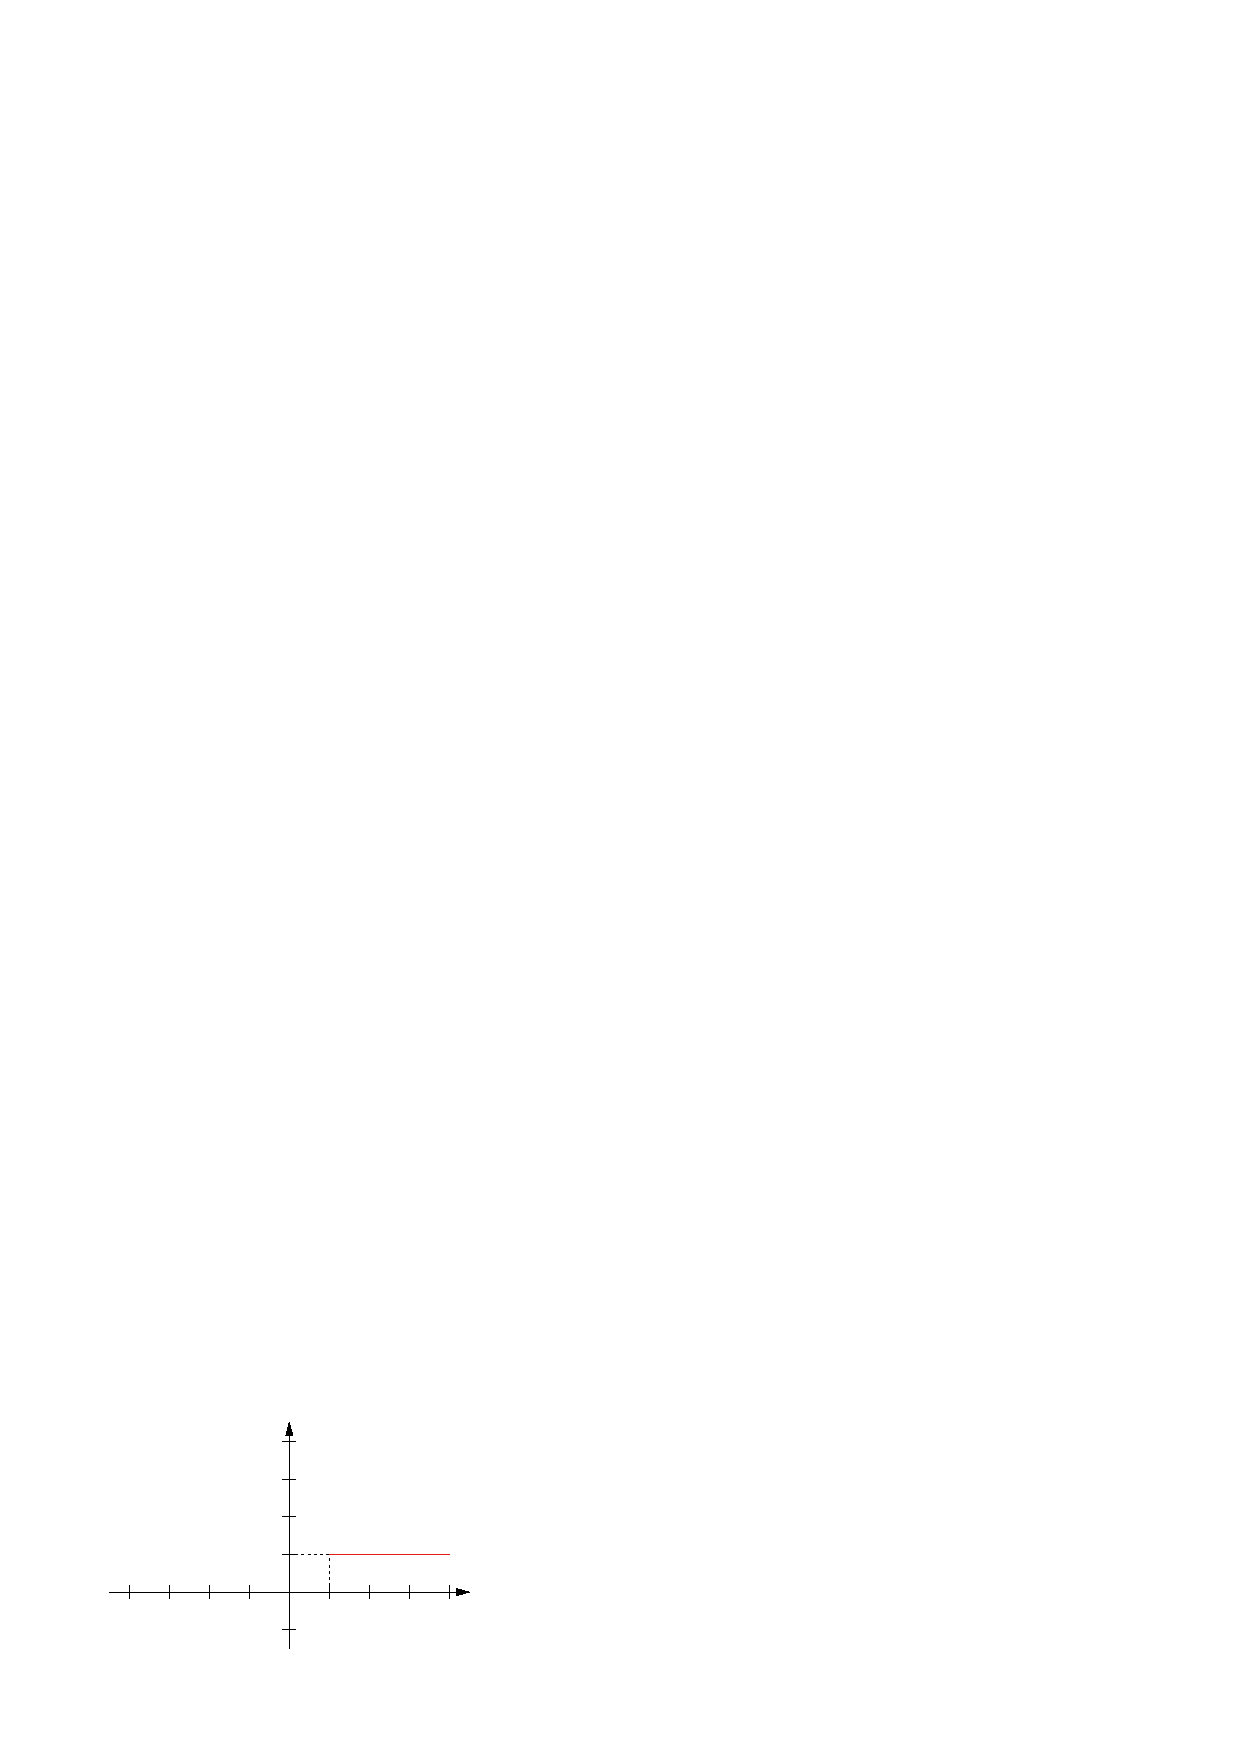
\includegraphics[width={180.00bp},height={108.00bp}]{figura_03_16}}%
    \gplfronttext
  \end{picture}%
\endgroup

    \end{minipage}
    \begin{minipage}{.4\textwidth}
        \centering
        % GNUPLOT: LaTeX picture with Postscript
\begingroup
  \makeatletter
  \providecommand\color[2][]{%
    \GenericError{(gnuplot) \space\space\space\@spaces}{%
      Package color not loaded in conjunction with
      terminal option `colourtext'%
    }{See the gnuplot documentation for explanation.%
    }{Either use 'blacktext' in gnuplot or load the package
      color.sty in LaTeX.}%
    \renewcommand\color[2][]{}%
  }%
  \providecommand\includegraphics[2][]{%
    \GenericError{(gnuplot) \space\space\space\@spaces}{%
      Package graphicx or graphics not loaded%
    }{See the gnuplot documentation for explanation.%
    }{The gnuplot epslatex terminal needs graphicx.sty or graphics.sty.}%
    \renewcommand\includegraphics[2][]{}%
  }%
  \providecommand\rotatebox[2]{#2}%
  \@ifundefined{ifGPcolor}{%
    \newif\ifGPcolor
    \GPcolorfalse
  }{}%
  \@ifundefined{ifGPblacktext}{%
    \newif\ifGPblacktext
    \GPblacktexttrue
  }{}%
  % define a \g@addto@macro without @ in the name:
  \let\gplgaddtomacro\g@addto@macro
  % define empty templates for all commands taking text:
  \gdef\gplbacktext{}%
  \gdef\gplfronttext{}%
  \makeatother
  \ifGPblacktext
    % no textcolor at all
    \def\colorrgb#1{}%
    \def\colorgray#1{}%
  \else
    % gray or color?
    \ifGPcolor
      \def\colorrgb#1{\color[rgb]{#1}}%
      \def\colorgray#1{\color[gray]{#1}}%
      \expandafter\def\csname LTw\endcsname{\color{white}}%
      \expandafter\def\csname LTb\endcsname{\color{black}}%
      \expandafter\def\csname LTa\endcsname{\color{black}}%
      \expandafter\def\csname LT0\endcsname{\color[rgb]{1,0,0}}%
      \expandafter\def\csname LT1\endcsname{\color[rgb]{0,1,0}}%
      \expandafter\def\csname LT2\endcsname{\color[rgb]{0,0,1}}%
      \expandafter\def\csname LT3\endcsname{\color[rgb]{1,0,1}}%
      \expandafter\def\csname LT4\endcsname{\color[rgb]{0,1,1}}%
      \expandafter\def\csname LT5\endcsname{\color[rgb]{1,1,0}}%
      \expandafter\def\csname LT6\endcsname{\color[rgb]{0,0,0}}%
      \expandafter\def\csname LT7\endcsname{\color[rgb]{1,0.3,0}}%
      \expandafter\def\csname LT8\endcsname{\color[rgb]{0.5,0.5,0.5}}%
    \else
      % gray
      \def\colorrgb#1{\color{black}}%
      \def\colorgray#1{\color[gray]{#1}}%
      \expandafter\def\csname LTw\endcsname{\color{white}}%
      \expandafter\def\csname LTb\endcsname{\color{black}}%
      \expandafter\def\csname LTa\endcsname{\color{black}}%
      \expandafter\def\csname LT0\endcsname{\color{black}}%
      \expandafter\def\csname LT1\endcsname{\color{black}}%
      \expandafter\def\csname LT2\endcsname{\color{black}}%
      \expandafter\def\csname LT3\endcsname{\color{black}}%
      \expandafter\def\csname LT4\endcsname{\color{black}}%
      \expandafter\def\csname LT5\endcsname{\color{black}}%
      \expandafter\def\csname LT6\endcsname{\color{black}}%
      \expandafter\def\csname LT7\endcsname{\color{black}}%
      \expandafter\def\csname LT8\endcsname{\color{black}}%
    \fi
  \fi
    \setlength{\unitlength}{0.0500bp}%
    \ifx\gptboxheight\undefined%
      \newlength{\gptboxheight}%
      \newlength{\gptboxwidth}%
      \newsavebox{\gptboxtext}%
    \fi%
    \setlength{\fboxrule}{0.5pt}%
    \setlength{\fboxsep}{1pt}%
    \definecolor{tbcol}{rgb}{1,1,1}%
\begin{picture}(3600.00,2160.00)%
    \gplgaddtomacro\gplbacktext{%
      \csname LTb\endcsname%%
      \put(1680,192){\makebox(0,0)[r]{\strut{}}}%
      \put(1680,553){\makebox(0,0)[r]{\strut{}}}%
      \put(1680,915){\makebox(0,0)[r]{\strut{}}}%
      \put(1680,1276){\makebox(0,0)[r]{\strut{}}}%
      \put(1680,1638){\makebox(0,0)[r]{\strut{}}}%
      \put(1680,1999){\makebox(0,0)[r]{\strut{}}}%
      \put(240,330){\makebox(0,0){\strut{}}}%
      \put(624,330){\makebox(0,0){\strut{}}}%
      \put(1008,330){\makebox(0,0){\strut{}}}%
      \put(1392,330){\makebox(0,0){\strut{}}}%
      \put(1776,330){\makebox(0,0){\strut{}}}%
      \put(2159,330){\makebox(0,0){\strut{}}}%
      \put(2543,330){\makebox(0,0){\strut{}}}%
      \put(2927,330){\makebox(0,0){\strut{}}}%
      \put(3311,330){\makebox(0,0){\strut{}}}%
      \csname LTb\endcsname%%
      \put(3580,553){\makebox(0,0)[l]{\strut{}$t$}}%
      \put(1219,2107){\makebox(0,0)[l]{\strut{}$f^\prime(t)$}}%
      \put(2121,337){\makebox(0,0)[l]{\strut{}$t_0$}}%
      \put(2313,1276){\makebox(0,0)[l]{\strut{}$\delta(t-t_0)$}}%
    }%
    \gplgaddtomacro\gplfronttext{%
    }%
    \gplbacktext
    \put(0,0){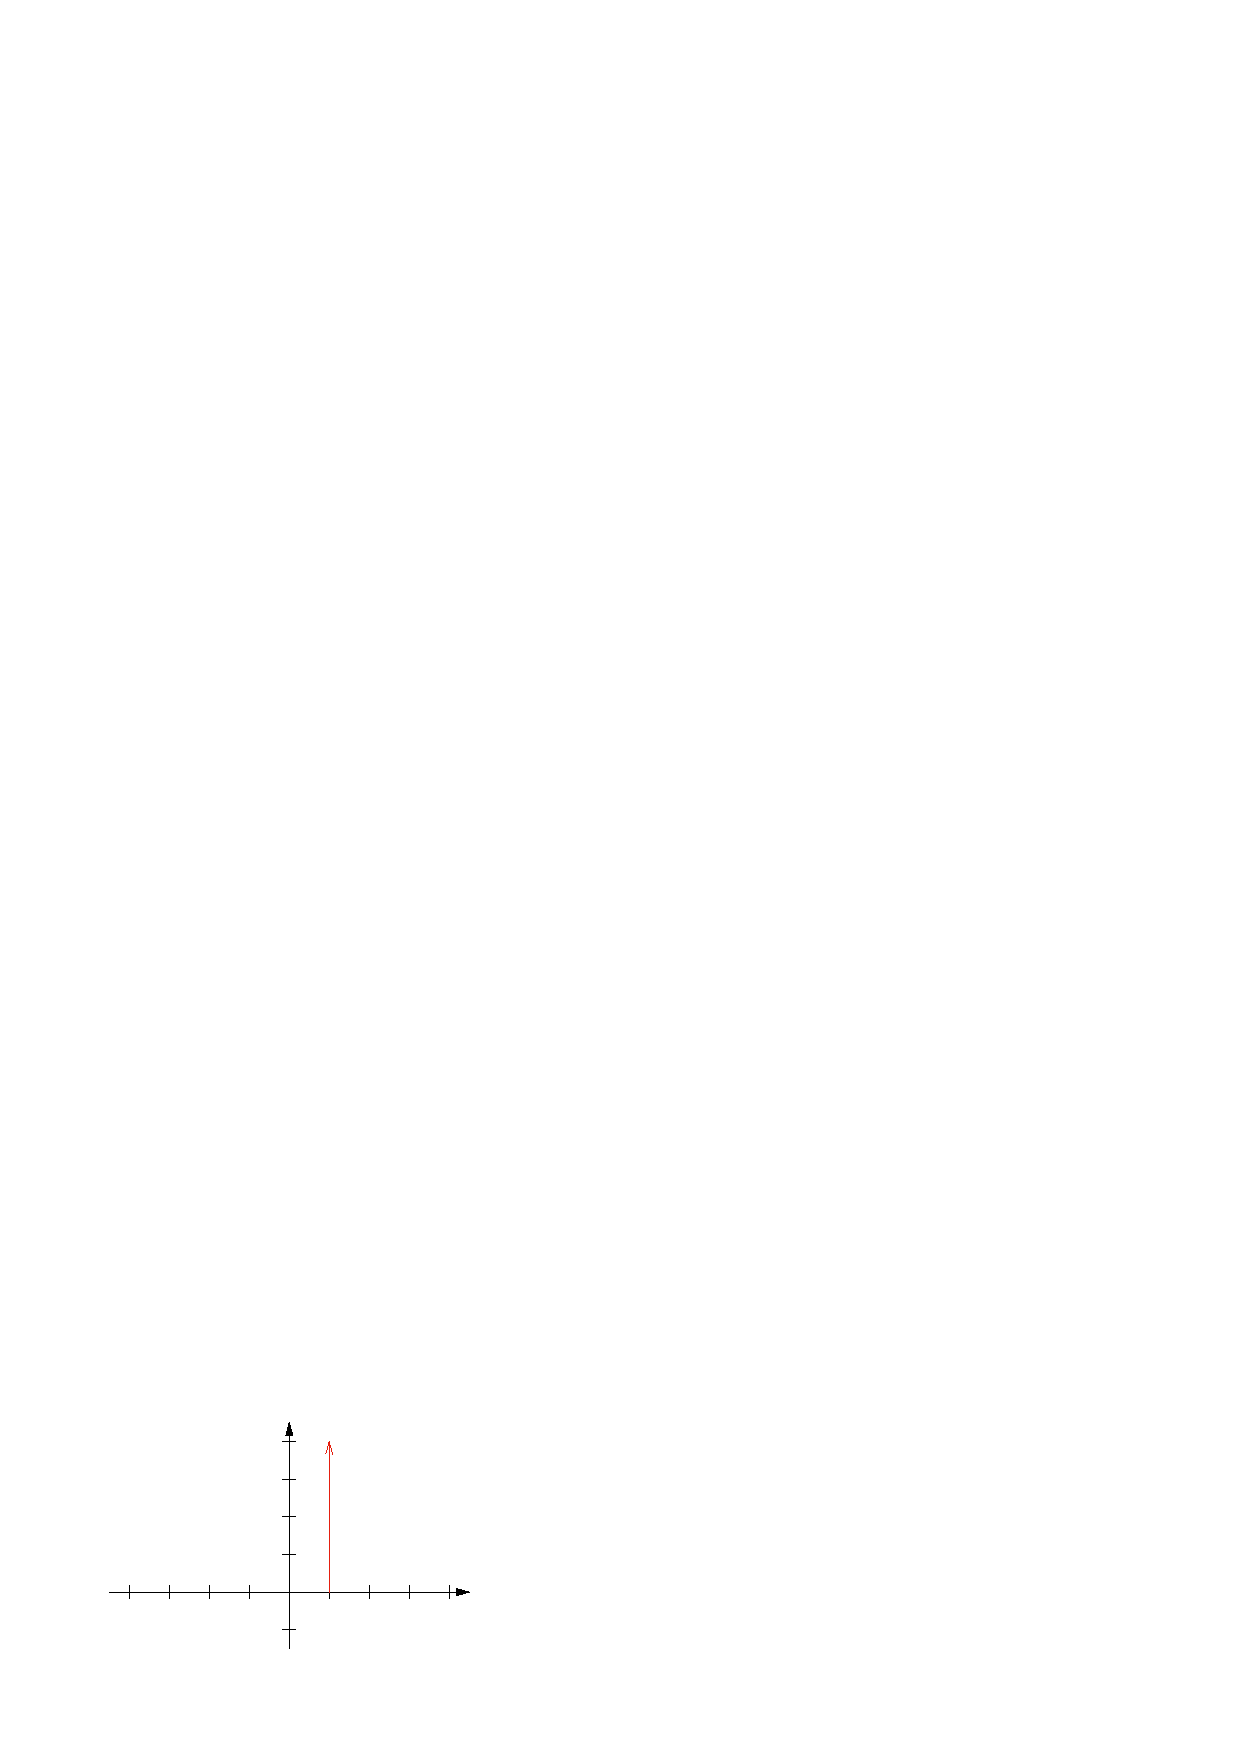
\includegraphics[width={180.00bp},height={108.00bp}]{figura_03_17}}%
    \gplfronttext
  \end{picture}%
\endgroup

    \end{minipage}
\end{figure}
\begin{equation}
    u'(t-t_0)=\delta(t-t_0)
\end{equation}

\underline{Prueba}:

\begin{equation*}
    \int_{-\infty}^{\infty}u'(t)\phi(t)\,dt
\end{equation*}

Realizando la integración por partes:
\begin{equation*}
    u=\phi(t)
\end{equation*}
\begin{equation*}
    du=\phi'(t)\,dt
\end{equation*}
\begin{equation*}
    dv=u'(t)\,dt
\end{equation*}
\begin{equation*}
    v=u(t)
\end{equation*}
\begin{equation*}
\begin{split}
    \int_{-\infty}^{\infty}\phi(t)u'(t)\,dt
        &=(\phi(t)u(t)\Big|_{-\infty}^{\infty})
        -\int_{-\infty}^{\infty}u(t)\phi'(t)\,dt\\
        &=-\int_{-\infty}^{\infty}u(t)\phi'(t)\,dt\\
        &=-\int_{0}^{\infty}1\,\phi'(t)\,dt\\
        &=-\phi(t)\Big|_0^{\infty}\\
        &=-\phi(\infty)+\phi(0)\\
\end{split}
\end{equation*}

Asumiendo que $\phi(\pm\infty)=0$:
\begin{equation*}
    \int_{-\infty}^{\infty}\phi(t)u'(t)\,dt=\phi(0)
\end{equation*}

Sabiendo que:
\begin{equation*}
    \int_{-\infty}^{\infty}\phi(t)\delta(t)\,dt=\phi(0)
\end{equation*}

Por tanto:
\begin{equation*}
    \int_{-\infty}^{\infty}\phi(t)u'(t)\,dt
        =\int_{-\infty}^{\infty}\phi(t)\delta(t)\,dt
\end{equation*}
\begin{equation*}
    \phi(t)u'(t)=\phi(t)\delta(t)
\end{equation*}
\begin{equation*}
    u'(t)=\delta(t)
\end{equation*}

\section{Derivada de una función con discontinuidades de salto}
Las derivadas de los saltos de subida y bajada, van a originar impulsos hacia
arriba y hacia abajo, respectivamente.
\begin{figure}[H]
    \centering
    \begin{minipage}{.4\textwidth}
        \centering
        % GNUPLOT: LaTeX picture with Postscript
\begingroup
  \makeatletter
  \providecommand\color[2][]{%
    \GenericError{(gnuplot) \space\space\space\@spaces}{%
      Package color not loaded in conjunction with
      terminal option `colourtext'%
    }{See the gnuplot documentation for explanation.%
    }{Either use 'blacktext' in gnuplot or load the package
      color.sty in LaTeX.}%
    \renewcommand\color[2][]{}%
  }%
  \providecommand\includegraphics[2][]{%
    \GenericError{(gnuplot) \space\space\space\@spaces}{%
      Package graphicx or graphics not loaded%
    }{See the gnuplot documentation for explanation.%
    }{The gnuplot epslatex terminal needs graphicx.sty or graphics.sty.}%
    \renewcommand\includegraphics[2][]{}%
  }%
  \providecommand\rotatebox[2]{#2}%
  \@ifundefined{ifGPcolor}{%
    \newif\ifGPcolor
    \GPcolorfalse
  }{}%
  \@ifundefined{ifGPblacktext}{%
    \newif\ifGPblacktext
    \GPblacktexttrue
  }{}%
  % define a \g@addto@macro without @ in the name:
  \let\gplgaddtomacro\g@addto@macro
  % define empty templates for all commands taking text:
  \gdef\gplbacktext{}%
  \gdef\gplfronttext{}%
  \makeatother
  \ifGPblacktext
    % no textcolor at all
    \def\colorrgb#1{}%
    \def\colorgray#1{}%
  \else
    % gray or color?
    \ifGPcolor
      \def\colorrgb#1{\color[rgb]{#1}}%
      \def\colorgray#1{\color[gray]{#1}}%
      \expandafter\def\csname LTw\endcsname{\color{white}}%
      \expandafter\def\csname LTb\endcsname{\color{black}}%
      \expandafter\def\csname LTa\endcsname{\color{black}}%
      \expandafter\def\csname LT0\endcsname{\color[rgb]{1,0,0}}%
      \expandafter\def\csname LT1\endcsname{\color[rgb]{0,1,0}}%
      \expandafter\def\csname LT2\endcsname{\color[rgb]{0,0,1}}%
      \expandafter\def\csname LT3\endcsname{\color[rgb]{1,0,1}}%
      \expandafter\def\csname LT4\endcsname{\color[rgb]{0,1,1}}%
      \expandafter\def\csname LT5\endcsname{\color[rgb]{1,1,0}}%
      \expandafter\def\csname LT6\endcsname{\color[rgb]{0,0,0}}%
      \expandafter\def\csname LT7\endcsname{\color[rgb]{1,0.3,0}}%
      \expandafter\def\csname LT8\endcsname{\color[rgb]{0.5,0.5,0.5}}%
    \else
      % gray
      \def\colorrgb#1{\color{black}}%
      \def\colorgray#1{\color[gray]{#1}}%
      \expandafter\def\csname LTw\endcsname{\color{white}}%
      \expandafter\def\csname LTb\endcsname{\color{black}}%
      \expandafter\def\csname LTa\endcsname{\color{black}}%
      \expandafter\def\csname LT0\endcsname{\color{black}}%
      \expandafter\def\csname LT1\endcsname{\color{black}}%
      \expandafter\def\csname LT2\endcsname{\color{black}}%
      \expandafter\def\csname LT3\endcsname{\color{black}}%
      \expandafter\def\csname LT4\endcsname{\color{black}}%
      \expandafter\def\csname LT5\endcsname{\color{black}}%
      \expandafter\def\csname LT6\endcsname{\color{black}}%
      \expandafter\def\csname LT7\endcsname{\color{black}}%
      \expandafter\def\csname LT8\endcsname{\color{black}}%
    \fi
  \fi
    \setlength{\unitlength}{0.0500bp}%
    \ifx\gptboxheight\undefined%
      \newlength{\gptboxheight}%
      \newlength{\gptboxwidth}%
      \newsavebox{\gptboxtext}%
    \fi%
    \setlength{\fboxrule}{0.5pt}%
    \setlength{\fboxsep}{1pt}%
    \definecolor{tbcol}{rgb}{1,1,1}%
\begin{picture}(3600.00,2160.00)%
    \gplgaddtomacro\gplbacktext{%
      \csname LTb\endcsname%%
      \put(1680,192){\makebox(0,0)[r]{\strut{}}}%
      \put(1680,553){\makebox(0,0)[r]{\strut{}}}%
      \put(1680,915){\makebox(0,0)[r]{\strut{}}}%
      \put(1680,1276){\makebox(0,0)[r]{\strut{}}}%
      \put(1680,1638){\makebox(0,0)[r]{\strut{}}}%
      \put(1680,1999){\makebox(0,0)[r]{\strut{}}}%
      \put(240,330){\makebox(0,0){\strut{}}}%
      \put(624,330){\makebox(0,0){\strut{}}}%
      \put(1008,330){\makebox(0,0){\strut{}}}%
      \put(1392,330){\makebox(0,0){\strut{}}}%
      \put(1776,330){\makebox(0,0){\strut{}}}%
      \put(2159,330){\makebox(0,0){\strut{}}}%
      \put(2543,330){\makebox(0,0){\strut{}}}%
      \put(2927,330){\makebox(0,0){\strut{}}}%
      \put(3311,330){\makebox(0,0){\strut{}}}%
      \csname LTb\endcsname%%
      \put(3580,553){\makebox(0,0)[l]{\strut{}$t$}}%
      \put(1219,2107){\makebox(0,0)[l]{\strut{}$f(t)$}}%
      \put(2121,337){\makebox(0,0)[l]{\strut{}$t_1$}}%
      \put(2889,337){\makebox(0,0)[l]{\strut{}$t_2$}}%
      \put(1488,734){\makebox(0,0)[l]{\strut{}$k_0$}}%
      \put(2255,1096){\makebox(0,0)[l]{\strut{}$k_1$}}%
      \put(2639,1096){\makebox(0,0)[l]{\strut{}$k_2$}}%
      \put(2543,1999){\makebox(0,0)[l]{\strut{}salto de bajada}}%
      \put(2927,1638){\makebox(0,0)[l]{\strut{}salto de subida}}%
    }%
    \gplgaddtomacro\gplfronttext{%
    }%
    \gplgaddtomacro\gplbacktext{%
      \csname LTb\endcsname%%
      \put(1680,192){\makebox(0,0)[r]{\strut{}}}%
      \put(1680,553){\makebox(0,0)[r]{\strut{}}}%
      \put(1680,915){\makebox(0,0)[r]{\strut{}}}%
      \put(1680,1276){\makebox(0,0)[r]{\strut{}}}%
      \put(1680,1638){\makebox(0,0)[r]{\strut{}}}%
      \put(1680,1999){\makebox(0,0)[r]{\strut{}}}%
      \put(240,330){\makebox(0,0){\strut{}}}%
      \put(624,330){\makebox(0,0){\strut{}}}%
      \put(1008,330){\makebox(0,0){\strut{}}}%
      \put(1392,330){\makebox(0,0){\strut{}}}%
      \put(1776,330){\makebox(0,0){\strut{}}}%
      \put(2159,330){\makebox(0,0){\strut{}}}%
      \put(2543,330){\makebox(0,0){\strut{}}}%
      \put(2927,330){\makebox(0,0){\strut{}}}%
      \put(3311,330){\makebox(0,0){\strut{}}}%
      \csname LTb\endcsname%%
      \put(3580,553){\makebox(0,0)[l]{\strut{}$t$}}%
      \put(1219,2107){\makebox(0,0)[l]{\strut{}$f(t)$}}%
      \put(2121,337){\makebox(0,0)[l]{\strut{}$t_1$}}%
      \put(2889,337){\makebox(0,0)[l]{\strut{}$t_2$}}%
      \put(1488,734){\makebox(0,0)[l]{\strut{}$k_0$}}%
      \put(2255,1096){\makebox(0,0)[l]{\strut{}$k_1$}}%
      \put(2639,1096){\makebox(0,0)[l]{\strut{}$k_2$}}%
      \put(2543,1999){\makebox(0,0)[l]{\strut{}salto de bajada}}%
      \put(2927,1638){\makebox(0,0)[l]{\strut{}salto de subida}}%
    }%
    \gplgaddtomacro\gplfronttext{%
    }%
    \gplgaddtomacro\gplbacktext{%
      \csname LTb\endcsname%%
      \put(1680,192){\makebox(0,0)[r]{\strut{}}}%
      \put(1680,553){\makebox(0,0)[r]{\strut{}}}%
      \put(1680,915){\makebox(0,0)[r]{\strut{}}}%
      \put(1680,1276){\makebox(0,0)[r]{\strut{}}}%
      \put(1680,1638){\makebox(0,0)[r]{\strut{}}}%
      \put(1680,1999){\makebox(0,0)[r]{\strut{}}}%
      \put(240,330){\makebox(0,0){\strut{}}}%
      \put(624,330){\makebox(0,0){\strut{}}}%
      \put(1008,330){\makebox(0,0){\strut{}}}%
      \put(1392,330){\makebox(0,0){\strut{}}}%
      \put(1776,330){\makebox(0,0){\strut{}}}%
      \put(2159,330){\makebox(0,0){\strut{}}}%
      \put(2543,330){\makebox(0,0){\strut{}}}%
      \put(2927,330){\makebox(0,0){\strut{}}}%
      \put(3311,330){\makebox(0,0){\strut{}}}%
      \csname LTb\endcsname%%
      \put(3580,553){\makebox(0,0)[l]{\strut{}$t$}}%
      \put(1219,2107){\makebox(0,0)[l]{\strut{}$f(t)$}}%
      \put(2121,337){\makebox(0,0)[l]{\strut{}$t_1$}}%
      \put(2889,337){\makebox(0,0)[l]{\strut{}$t_2$}}%
      \put(1488,734){\makebox(0,0)[l]{\strut{}$k_0$}}%
      \put(2255,1096){\makebox(0,0)[l]{\strut{}$k_1$}}%
      \put(2639,1096){\makebox(0,0)[l]{\strut{}$k_2$}}%
      \put(2543,1999){\makebox(0,0)[l]{\strut{}salto de bajada}}%
      \put(2927,1638){\makebox(0,0)[l]{\strut{}salto de subida}}%
    }%
    \gplgaddtomacro\gplfronttext{%
    }%
    \gplbacktext
    \put(0,0){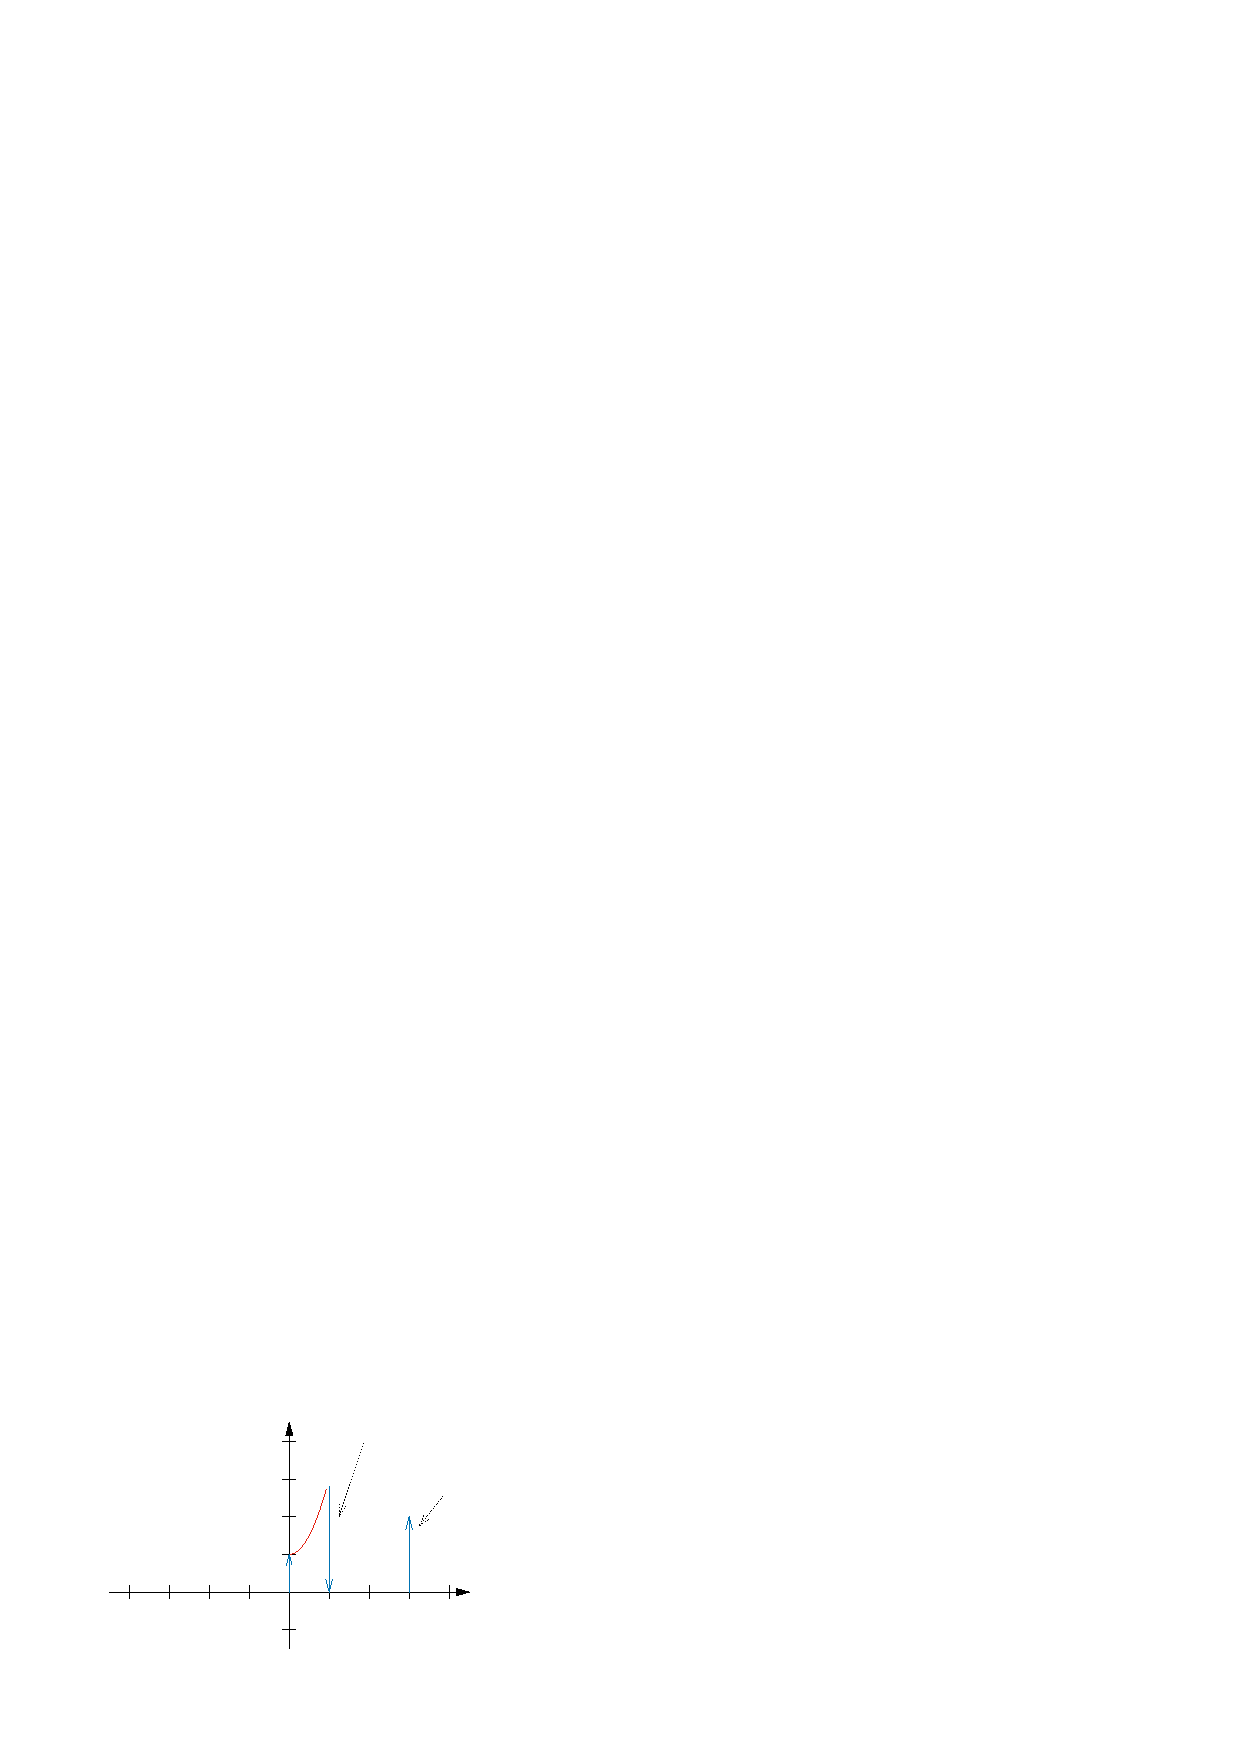
\includegraphics[width={180.00bp},height={108.00bp}]{figura_03_18}}%
    \gplfronttext
  \end{picture}%
\endgroup

    \end{minipage}
    \begin{minipage}{.4\textwidth}
        \centering
        % GNUPLOT: LaTeX picture with Postscript
\begingroup
  \makeatletter
  \providecommand\color[2][]{%
    \GenericError{(gnuplot) \space\space\space\@spaces}{%
      Package color not loaded in conjunction with
      terminal option `colourtext'%
    }{See the gnuplot documentation for explanation.%
    }{Either use 'blacktext' in gnuplot or load the package
      color.sty in LaTeX.}%
    \renewcommand\color[2][]{}%
  }%
  \providecommand\includegraphics[2][]{%
    \GenericError{(gnuplot) \space\space\space\@spaces}{%
      Package graphicx or graphics not loaded%
    }{See the gnuplot documentation for explanation.%
    }{The gnuplot epslatex terminal needs graphicx.sty or graphics.sty.}%
    \renewcommand\includegraphics[2][]{}%
  }%
  \providecommand\rotatebox[2]{#2}%
  \@ifundefined{ifGPcolor}{%
    \newif\ifGPcolor
    \GPcolorfalse
  }{}%
  \@ifundefined{ifGPblacktext}{%
    \newif\ifGPblacktext
    \GPblacktexttrue
  }{}%
  % define a \g@addto@macro without @ in the name:
  \let\gplgaddtomacro\g@addto@macro
  % define empty templates for all commands taking text:
  \gdef\gplbacktext{}%
  \gdef\gplfronttext{}%
  \makeatother
  \ifGPblacktext
    % no textcolor at all
    \def\colorrgb#1{}%
    \def\colorgray#1{}%
  \else
    % gray or color?
    \ifGPcolor
      \def\colorrgb#1{\color[rgb]{#1}}%
      \def\colorgray#1{\color[gray]{#1}}%
      \expandafter\def\csname LTw\endcsname{\color{white}}%
      \expandafter\def\csname LTb\endcsname{\color{black}}%
      \expandafter\def\csname LTa\endcsname{\color{black}}%
      \expandafter\def\csname LT0\endcsname{\color[rgb]{1,0,0}}%
      \expandafter\def\csname LT1\endcsname{\color[rgb]{0,1,0}}%
      \expandafter\def\csname LT2\endcsname{\color[rgb]{0,0,1}}%
      \expandafter\def\csname LT3\endcsname{\color[rgb]{1,0,1}}%
      \expandafter\def\csname LT4\endcsname{\color[rgb]{0,1,1}}%
      \expandafter\def\csname LT5\endcsname{\color[rgb]{1,1,0}}%
      \expandafter\def\csname LT6\endcsname{\color[rgb]{0,0,0}}%
      \expandafter\def\csname LT7\endcsname{\color[rgb]{1,0.3,0}}%
      \expandafter\def\csname LT8\endcsname{\color[rgb]{0.5,0.5,0.5}}%
    \else
      % gray
      \def\colorrgb#1{\color{black}}%
      \def\colorgray#1{\color[gray]{#1}}%
      \expandafter\def\csname LTw\endcsname{\color{white}}%
      \expandafter\def\csname LTb\endcsname{\color{black}}%
      \expandafter\def\csname LTa\endcsname{\color{black}}%
      \expandafter\def\csname LT0\endcsname{\color{black}}%
      \expandafter\def\csname LT1\endcsname{\color{black}}%
      \expandafter\def\csname LT2\endcsname{\color{black}}%
      \expandafter\def\csname LT3\endcsname{\color{black}}%
      \expandafter\def\csname LT4\endcsname{\color{black}}%
      \expandafter\def\csname LT5\endcsname{\color{black}}%
      \expandafter\def\csname LT6\endcsname{\color{black}}%
      \expandafter\def\csname LT7\endcsname{\color{black}}%
      \expandafter\def\csname LT8\endcsname{\color{black}}%
    \fi
  \fi
    \setlength{\unitlength}{0.0500bp}%
    \ifx\gptboxheight\undefined%
      \newlength{\gptboxheight}%
      \newlength{\gptboxwidth}%
      \newsavebox{\gptboxtext}%
    \fi%
    \setlength{\fboxrule}{0.5pt}%
    \setlength{\fboxsep}{1pt}%
    \definecolor{tbcol}{rgb}{1,1,1}%
\begin{picture}(3600.00,2160.00)%
    \gplgaddtomacro\gplbacktext{%
      \csname LTb\endcsname%%
      \put(1680,192){\makebox(0,0)[r]{\strut{}}}%
      \put(1680,553){\makebox(0,0)[r]{\strut{}}}%
      \put(1680,915){\makebox(0,0)[r]{\strut{}}}%
      \put(1680,1276){\makebox(0,0)[r]{\strut{}}}%
      \put(1680,1638){\makebox(0,0)[r]{\strut{}}}%
      \put(1680,1999){\makebox(0,0)[r]{\strut{}}}%
      \put(240,330){\makebox(0,0){\strut{}}}%
      \put(624,330){\makebox(0,0){\strut{}}}%
      \put(1008,330){\makebox(0,0){\strut{}}}%
      \put(1392,330){\makebox(0,0){\strut{}}}%
      \put(1776,330){\makebox(0,0){\strut{}}}%
      \put(2159,330){\makebox(0,0){\strut{}}}%
      \put(2543,330){\makebox(0,0){\strut{}}}%
      \put(2927,330){\makebox(0,0){\strut{}}}%
      \put(3311,330){\makebox(0,0){\strut{}}}%
      \csname LTb\endcsname%%
      \put(3580,553){\makebox(0,0)[l]{\strut{}$t$}}%
      \put(1219,2107){\makebox(0,0)[l]{\strut{}$f^\prime(t)$}}%
      \put(2121,337){\makebox(0,0)[l]{\strut{}$t_1$}}%
      \put(2889,337){\makebox(0,0)[l]{\strut{}$t_2$}}%
      \put(1871,734){\makebox(0,0)[l]{\strut{}$k_0\delta(t)$}}%
      \put(2255,11){\makebox(0,0)[l]{\strut{}$-k_1\delta(t-t_1)$}}%
      \put(3023,1005){\makebox(0,0)[l]{\strut{}$k_2\delta(t-t_2)$}}%
    }%
    \gplgaddtomacro\gplfronttext{%
    }%
    \gplbacktext
    \put(0,0){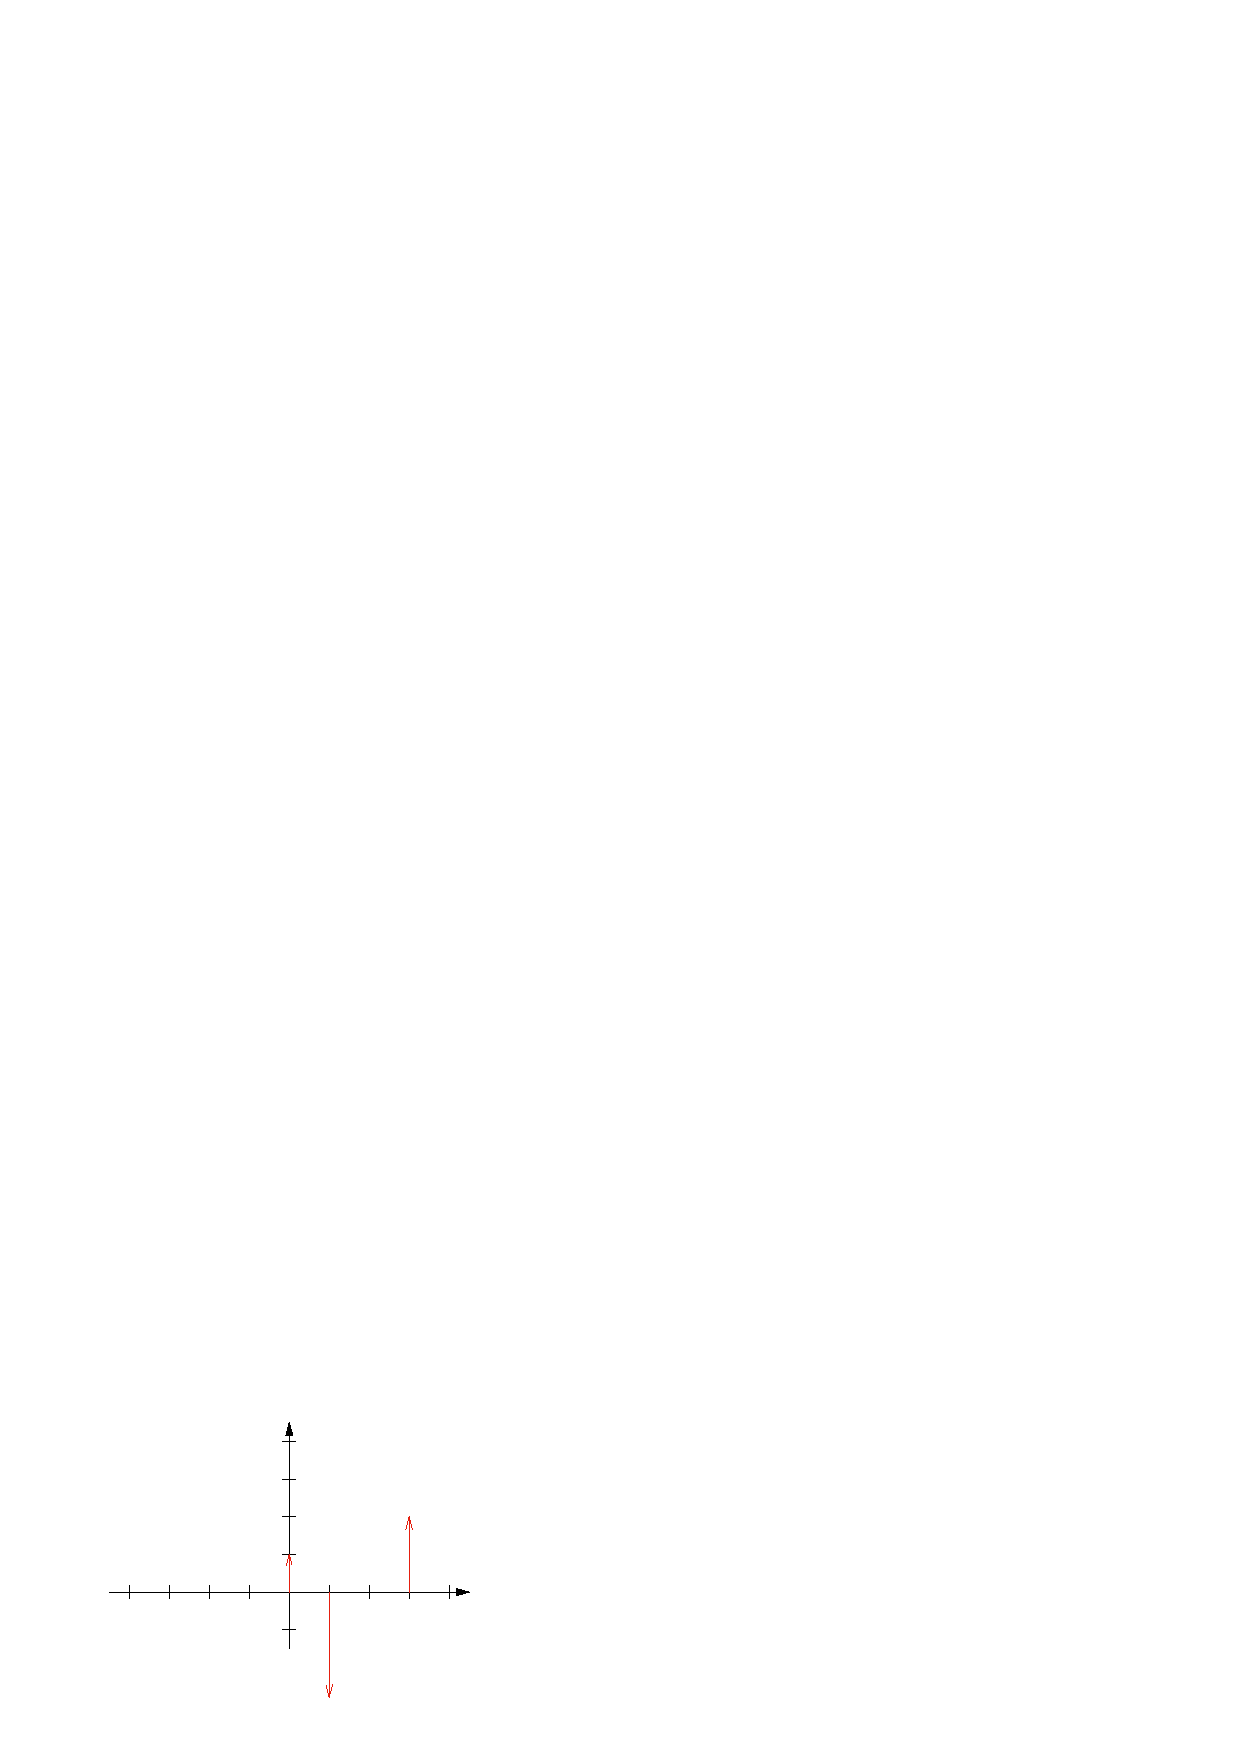
\includegraphics[width={180.00bp},height={108.00bp}]{figura_03_19}}%
    \gplfronttext
  \end{picture}%
\endgroup

    \end{minipage}
\end{figure}

\section{Series de \emph{Fourier} por el método de diferenciación}
\begin{minipage}{.5\linewidth}
    \begin{equation*}
        f(t)=\sum_{n=-\infty}^{\infty}c_n\,e^{jn\omega_0\,t}
    \end{equation*}
\end{minipage}
\begin{minipage}{.5\linewidth}
    \begin{equation*}
        c_n=\frac{1}{T}\int_0^T\,f(t)\,e^{-jn\omega_0\,t}\,dt
    \end{equation*}
\end{minipage}
\begin{minipage}{.5\linewidth}
    \begin{equation*}
        f^\prime(t)=\sum_{n=-\infty}^{\infty}jn\omega_0\,c_n\,e^{jn\omega_0\,t}
    \end{equation*}
\end{minipage}
\begin{minipage}{.5\linewidth}
    \begin{equation}
        \gamma^\prime_n=\frac{1}{T}\int_0^T\,f^\prime(t)\,e^{-jn\omega_0\,t}\,dt
    \end{equation}
\end{minipage}
\begin{minipage}{.5\linewidth}
    \begin{equation*}
        f^{\prime\prime}(t)
            =\sum_{n=-\infty}^{\infty}{(jn\omega_0)}^2\,c_n\,e^{jn\omega_0\,t}
    \end{equation*}
\end{minipage}
\begin{minipage}{.5\linewidth}
    \begin{equation}
        \gamma^{\prime\prime}_n
            =\frac{1}{T}\int_0^T\,f^{\prime\prime}(t)\,e^{-jn\omega_0\,t}\,dt
    \end{equation}
\end{minipage}
\begin{minipage}{.5\linewidth}
    \begin{equation*}
        f^{(k)}(t)
            =\sum_{n=-\infty}^{\infty}{(jn\omega_0)}^k\,c_n\,e^{jn\omega_0\,t}
    \end{equation*}
\end{minipage}
\begin{minipage}{.5\linewidth}
    \begin{equation}
        \gamma^{(k)}_n
            =\frac{1}{T}\int_0^T\,f^{(k)}(t)\,e^{-jn\omega_0\,t}\,dt
    \end{equation}
\end{minipage}

\begin{itemize}
    \item Se deriva $f(t)$ hasta anularla y calcular para cada derivada:
    $\gamma^{(k)}_n$
    \item Las derivadas de $f(t)$ solo van a tomar en cuenta los impulsos
    obtenidos de los saltos previos.
    \item El coeficiente complejo $c_n$ se obtendrá de la forma:
    \begin{equation}
        c_n=c^\prime_n+c^{\prime\prime}_n+\cdots+c^{(k)}_n
    \end{equation}
    Donde:
    \begin{equation}
        c^\prime_n=\frac{\gamma^\prime_n}{jn\omega_0}
    \end{equation}
    \begin{equation}
        c^{\prime\prime}_n=\frac{\gamma^{\prime\prime}_n}{{(jn\omega_0)}^2}
    \end{equation}
    \begin{equation}
        c^{(k)}_n=\frac{\gamma^{(k)}_n}{{(jn\omega_0)}^k}
    \end{equation}
\end{itemize}

\section{Espectros de frecuencia discreta}
Los espectros de frecuencia serán gráficas discretas de modulo y argumento del
coeficiente complejo de \emph{Fourier} en función de múltiplos de la frecuencia:
$\omega_0$.
\begin{equation*}
    f(t)=\sum_{n=-\infty}^\infty\,c_n\,e^{jn\omega_0\,t}
\end{equation*}
\begin{equation*}
    c_n=A_n+jB_n
\end{equation*}
\begin{equation*}
\left.\begin{aligned}
    |c_n|&=\sqrt{A_n^2+B_n^2}\\
    \theta_n&=\arctan\left(\frac{B_n}{A_n}\right)\\
\end{aligned}\right\}
\text{funciones discretas de }n\omega_0\quad\,n\in\mathbb{Z}
\end{equation*}
\begin{figure}[H]
    \centering
    \begin{minipage}{.4\textwidth}
        \centering
        % GNUPLOT: LaTeX picture with Postscript
\begingroup
  \makeatletter
  \providecommand\color[2][]{%
    \GenericError{(gnuplot) \space\space\space\@spaces}{%
      Package color not loaded in conjunction with
      terminal option `colourtext'%
    }{See the gnuplot documentation for explanation.%
    }{Either use 'blacktext' in gnuplot or load the package
      color.sty in LaTeX.}%
    \renewcommand\color[2][]{}%
  }%
  \providecommand\includegraphics[2][]{%
    \GenericError{(gnuplot) \space\space\space\@spaces}{%
      Package graphicx or graphics not loaded%
    }{See the gnuplot documentation for explanation.%
    }{The gnuplot epslatex terminal needs graphicx.sty or graphics.sty.}%
    \renewcommand\includegraphics[2][]{}%
  }%
  \providecommand\rotatebox[2]{#2}%
  \@ifundefined{ifGPcolor}{%
    \newif\ifGPcolor
    \GPcolorfalse
  }{}%
  \@ifundefined{ifGPblacktext}{%
    \newif\ifGPblacktext
    \GPblacktexttrue
  }{}%
  % define a \g@addto@macro without @ in the name:
  \let\gplgaddtomacro\g@addto@macro
  % define empty templates for all commands taking text:
  \gdef\gplbacktext{}%
  \gdef\gplfronttext{}%
  \makeatother
  \ifGPblacktext
    % no textcolor at all
    \def\colorrgb#1{}%
    \def\colorgray#1{}%
  \else
    % gray or color?
    \ifGPcolor
      \def\colorrgb#1{\color[rgb]{#1}}%
      \def\colorgray#1{\color[gray]{#1}}%
      \expandafter\def\csname LTw\endcsname{\color{white}}%
      \expandafter\def\csname LTb\endcsname{\color{black}}%
      \expandafter\def\csname LTa\endcsname{\color{black}}%
      \expandafter\def\csname LT0\endcsname{\color[rgb]{1,0,0}}%
      \expandafter\def\csname LT1\endcsname{\color[rgb]{0,1,0}}%
      \expandafter\def\csname LT2\endcsname{\color[rgb]{0,0,1}}%
      \expandafter\def\csname LT3\endcsname{\color[rgb]{1,0,1}}%
      \expandafter\def\csname LT4\endcsname{\color[rgb]{0,1,1}}%
      \expandafter\def\csname LT5\endcsname{\color[rgb]{1,1,0}}%
      \expandafter\def\csname LT6\endcsname{\color[rgb]{0,0,0}}%
      \expandafter\def\csname LT7\endcsname{\color[rgb]{1,0.3,0}}%
      \expandafter\def\csname LT8\endcsname{\color[rgb]{0.5,0.5,0.5}}%
    \else
      % gray
      \def\colorrgb#1{\color{black}}%
      \def\colorgray#1{\color[gray]{#1}}%
      \expandafter\def\csname LTw\endcsname{\color{white}}%
      \expandafter\def\csname LTb\endcsname{\color{black}}%
      \expandafter\def\csname LTa\endcsname{\color{black}}%
      \expandafter\def\csname LT0\endcsname{\color{black}}%
      \expandafter\def\csname LT1\endcsname{\color{black}}%
      \expandafter\def\csname LT2\endcsname{\color{black}}%
      \expandafter\def\csname LT3\endcsname{\color{black}}%
      \expandafter\def\csname LT4\endcsname{\color{black}}%
      \expandafter\def\csname LT5\endcsname{\color{black}}%
      \expandafter\def\csname LT6\endcsname{\color{black}}%
      \expandafter\def\csname LT7\endcsname{\color{black}}%
      \expandafter\def\csname LT8\endcsname{\color{black}}%
    \fi
  \fi
    \setlength{\unitlength}{0.0500bp}%
    \ifx\gptboxheight\undefined%
      \newlength{\gptboxheight}%
      \newlength{\gptboxwidth}%
      \newsavebox{\gptboxtext}%
    \fi%
    \setlength{\fboxrule}{0.5pt}%
    \setlength{\fboxsep}{1pt}%
    \definecolor{tbcol}{rgb}{1,1,1}%
\begin{picture}(3168.00,2160.00)%
    \gplgaddtomacro\gplbacktext{%
      \csname LTb\endcsname%%
      \put(1464,192){\makebox(0,0)[r]{\strut{}}}%
      \put(1464,553){\makebox(0,0)[r]{\strut{}}}%
      \put(1464,915){\makebox(0,0)[r]{\strut{}}}%
      \put(1464,1276){\makebox(0,0)[r]{\strut{}}}%
      \put(1464,1638){\makebox(0,0)[r]{\strut{}}}%
      \put(1464,1999){\makebox(0,0)[r]{\strut{}}}%
      \put(240,330){\makebox(0,0){\strut{}}}%
      \put(570,330){\makebox(0,0){\strut{}}}%
      \put(900,330){\makebox(0,0){\strut{}}}%
      \put(1230,330){\makebox(0,0){\strut{}}}%
      \put(1560,330){\makebox(0,0){\strut{}}}%
      \put(1889,330){\makebox(0,0){\strut{}}}%
      \put(2219,330){\makebox(0,0){\strut{}}}%
      \put(2549,330){\makebox(0,0){\strut{}}}%
      \put(2879,330){\makebox(0,0){\strut{}}}%
      \csname LTb\endcsname%%
      \put(3110,553){\makebox(0,0)[l]{\strut{}$n\omega_0$}}%
      \put(1081,2107){\makebox(0,0)[l]{\strut{}$|c_n|$}}%
      \put(273,337){\makebox(0,0)[l]{\strut{}$-3\omega_0$}}%
      \put(1032,337){\makebox(0,0)[l]{\strut{}$ -\omega_0$}}%
      \put(1856,337){\makebox(0,0)[l]{\strut{}$  \omega_0$}}%
      \put(2417,337){\makebox(0,0)[l]{\strut{}$ 3\omega_0$}}%
    }%
    \gplgaddtomacro\gplfronttext{%
    }%
    \gplbacktext
    \put(0,0){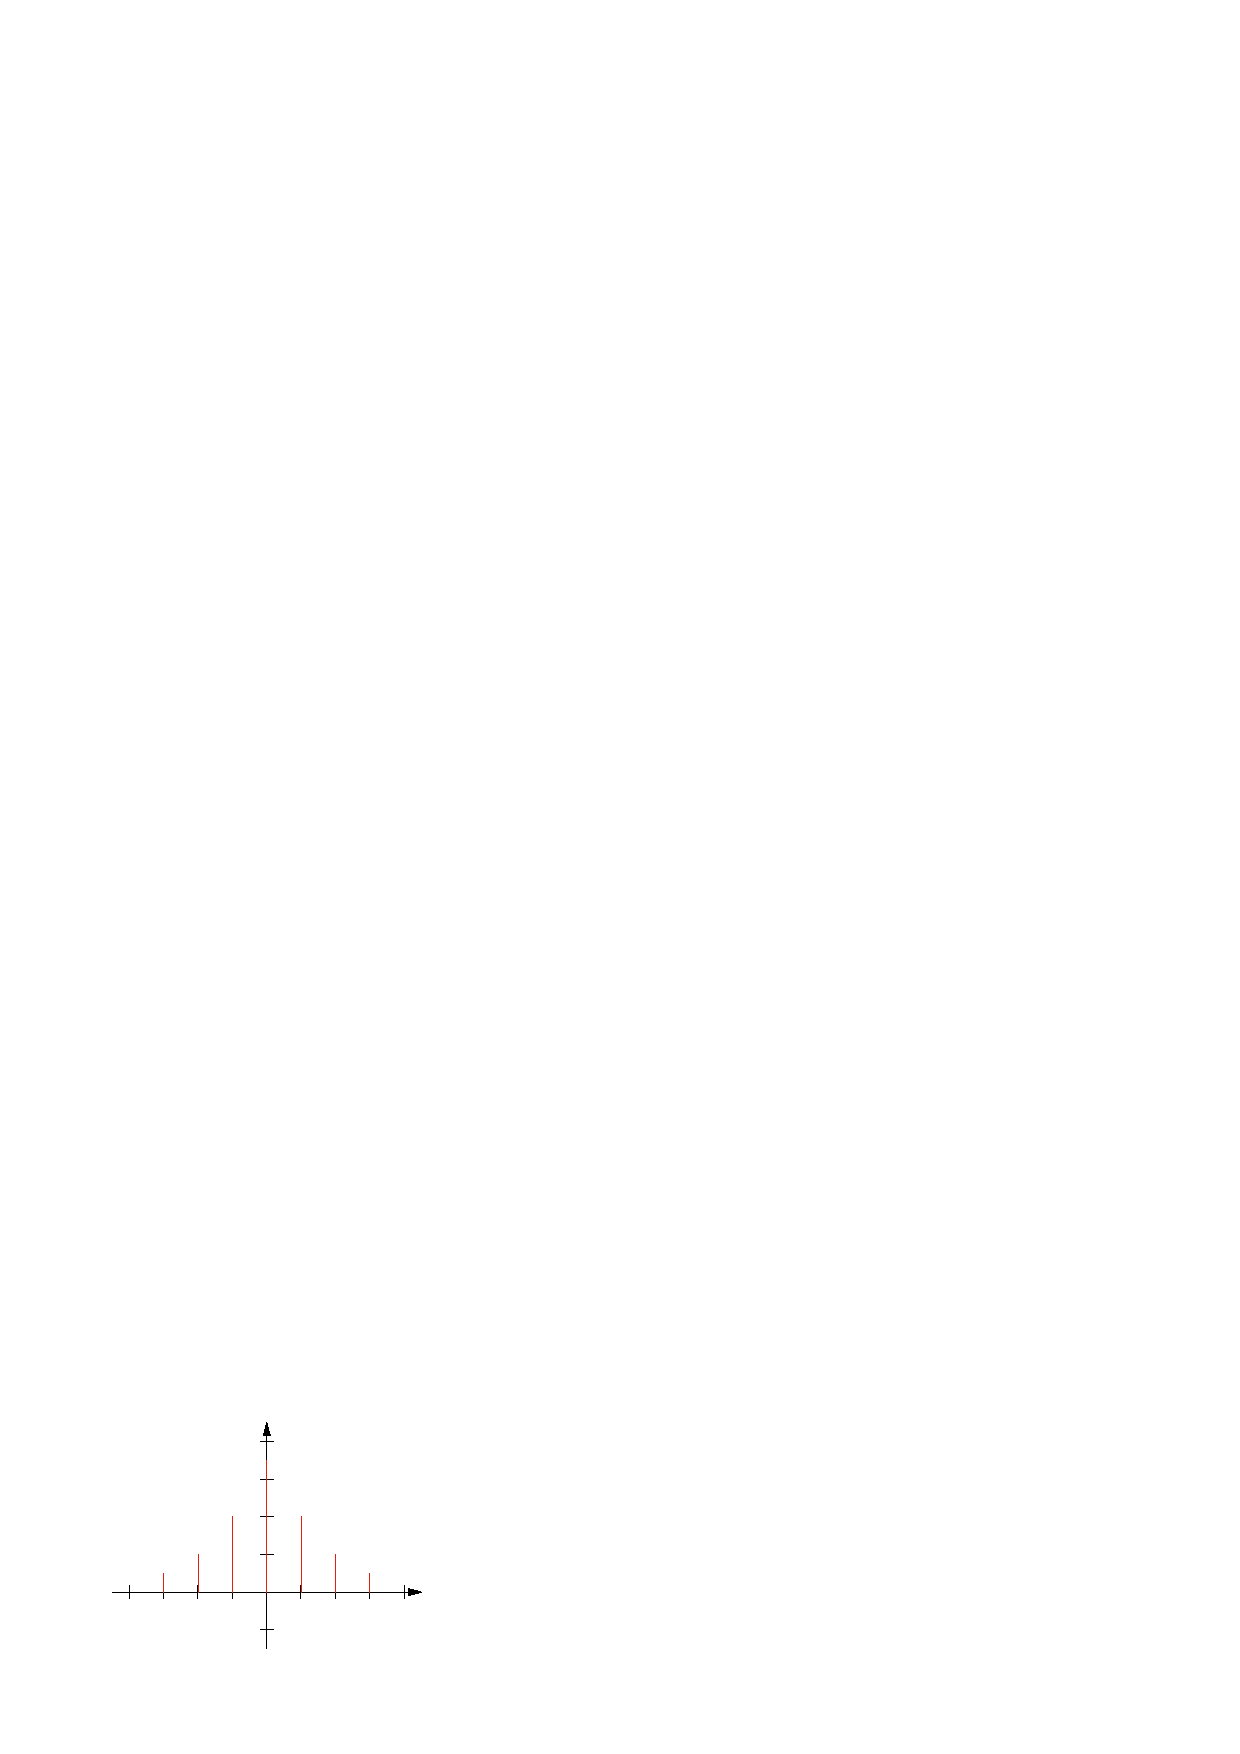
\includegraphics[width={158.40bp},height={108.00bp}]{figura_03_20}}%
    \gplfronttext
  \end{picture}%
\endgroup

        \captionsetup{labelformat=empty}
        \caption{Espectro de amplitud o módulo}
    \end{minipage}
    \begin{minipage}{.4\textwidth}
        \centering
        % GNUPLOT: LaTeX picture with Postscript
\begingroup
  \makeatletter
  \providecommand\color[2][]{%
    \GenericError{(gnuplot) \space\space\space\@spaces}{%
      Package color not loaded in conjunction with
      terminal option `colourtext'%
    }{See the gnuplot documentation for explanation.%
    }{Either use 'blacktext' in gnuplot or load the package
      color.sty in LaTeX.}%
    \renewcommand\color[2][]{}%
  }%
  \providecommand\includegraphics[2][]{%
    \GenericError{(gnuplot) \space\space\space\@spaces}{%
      Package graphicx or graphics not loaded%
    }{See the gnuplot documentation for explanation.%
    }{The gnuplot epslatex terminal needs graphicx.sty or graphics.sty.}%
    \renewcommand\includegraphics[2][]{}%
  }%
  \providecommand\rotatebox[2]{#2}%
  \@ifundefined{ifGPcolor}{%
    \newif\ifGPcolor
    \GPcolorfalse
  }{}%
  \@ifundefined{ifGPblacktext}{%
    \newif\ifGPblacktext
    \GPblacktexttrue
  }{}%
  % define a \g@addto@macro without @ in the name:
  \let\gplgaddtomacro\g@addto@macro
  % define empty templates for all commands taking text:
  \gdef\gplbacktext{}%
  \gdef\gplfronttext{}%
  \makeatother
  \ifGPblacktext
    % no textcolor at all
    \def\colorrgb#1{}%
    \def\colorgray#1{}%
  \else
    % gray or color?
    \ifGPcolor
      \def\colorrgb#1{\color[rgb]{#1}}%
      \def\colorgray#1{\color[gray]{#1}}%
      \expandafter\def\csname LTw\endcsname{\color{white}}%
      \expandafter\def\csname LTb\endcsname{\color{black}}%
      \expandafter\def\csname LTa\endcsname{\color{black}}%
      \expandafter\def\csname LT0\endcsname{\color[rgb]{1,0,0}}%
      \expandafter\def\csname LT1\endcsname{\color[rgb]{0,1,0}}%
      \expandafter\def\csname LT2\endcsname{\color[rgb]{0,0,1}}%
      \expandafter\def\csname LT3\endcsname{\color[rgb]{1,0,1}}%
      \expandafter\def\csname LT4\endcsname{\color[rgb]{0,1,1}}%
      \expandafter\def\csname LT5\endcsname{\color[rgb]{1,1,0}}%
      \expandafter\def\csname LT6\endcsname{\color[rgb]{0,0,0}}%
      \expandafter\def\csname LT7\endcsname{\color[rgb]{1,0.3,0}}%
      \expandafter\def\csname LT8\endcsname{\color[rgb]{0.5,0.5,0.5}}%
    \else
      % gray
      \def\colorrgb#1{\color{black}}%
      \def\colorgray#1{\color[gray]{#1}}%
      \expandafter\def\csname LTw\endcsname{\color{white}}%
      \expandafter\def\csname LTb\endcsname{\color{black}}%
      \expandafter\def\csname LTa\endcsname{\color{black}}%
      \expandafter\def\csname LT0\endcsname{\color{black}}%
      \expandafter\def\csname LT1\endcsname{\color{black}}%
      \expandafter\def\csname LT2\endcsname{\color{black}}%
      \expandafter\def\csname LT3\endcsname{\color{black}}%
      \expandafter\def\csname LT4\endcsname{\color{black}}%
      \expandafter\def\csname LT5\endcsname{\color{black}}%
      \expandafter\def\csname LT6\endcsname{\color{black}}%
      \expandafter\def\csname LT7\endcsname{\color{black}}%
      \expandafter\def\csname LT8\endcsname{\color{black}}%
    \fi
  \fi
    \setlength{\unitlength}{0.0500bp}%
    \ifx\gptboxheight\undefined%
      \newlength{\gptboxheight}%
      \newlength{\gptboxwidth}%
      \newsavebox{\gptboxtext}%
    \fi%
    \setlength{\fboxrule}{0.5pt}%
    \setlength{\fboxsep}{1pt}%
    \definecolor{tbcol}{rgb}{1,1,1}%
\begin{picture}(3168.00,2160.00)%
    \gplgaddtomacro\gplbacktext{%
      \csname LTb\endcsname%%
      \put(1464,192){\makebox(0,0)[r]{\strut{}}}%
      \put(1464,553){\makebox(0,0)[r]{\strut{}}}%
      \put(1464,915){\makebox(0,0)[r]{\strut{}}}%
      \put(1464,1276){\makebox(0,0)[r]{\strut{}}}%
      \put(1464,1638){\makebox(0,0)[r]{\strut{}}}%
      \put(1464,1999){\makebox(0,0)[r]{\strut{}}}%
      \put(240,330){\makebox(0,0){\strut{}}}%
      \put(570,330){\makebox(0,0){\strut{}}}%
      \put(900,330){\makebox(0,0){\strut{}}}%
      \put(1230,330){\makebox(0,0){\strut{}}}%
      \put(1560,330){\makebox(0,0){\strut{}}}%
      \put(1889,330){\makebox(0,0){\strut{}}}%
      \put(2219,330){\makebox(0,0){\strut{}}}%
      \put(2549,330){\makebox(0,0){\strut{}}}%
      \put(2879,330){\makebox(0,0){\strut{}}}%
      \csname LTb\endcsname%%
      \put(3110,553){\makebox(0,0)[l]{\strut{}$n\omega_0$}}%
      \put(1081,2107){\makebox(0,0)[l]{\strut{}$\theta_n$}}%
      \put(273,337){\makebox(0,0)[l]{\strut{}$-3\omega_0$}}%
      \put(1032,337){\makebox(0,0)[l]{\strut{}$ -\omega_0$}}%
      \put(1856,337){\makebox(0,0)[l]{\strut{}$  \omega_0$}}%
      \put(2417,337){\makebox(0,0)[l]{\strut{}$ 3\omega_0$}}%
    }%
    \gplgaddtomacro\gplfronttext{%
    }%
    \gplbacktext
    \put(0,0){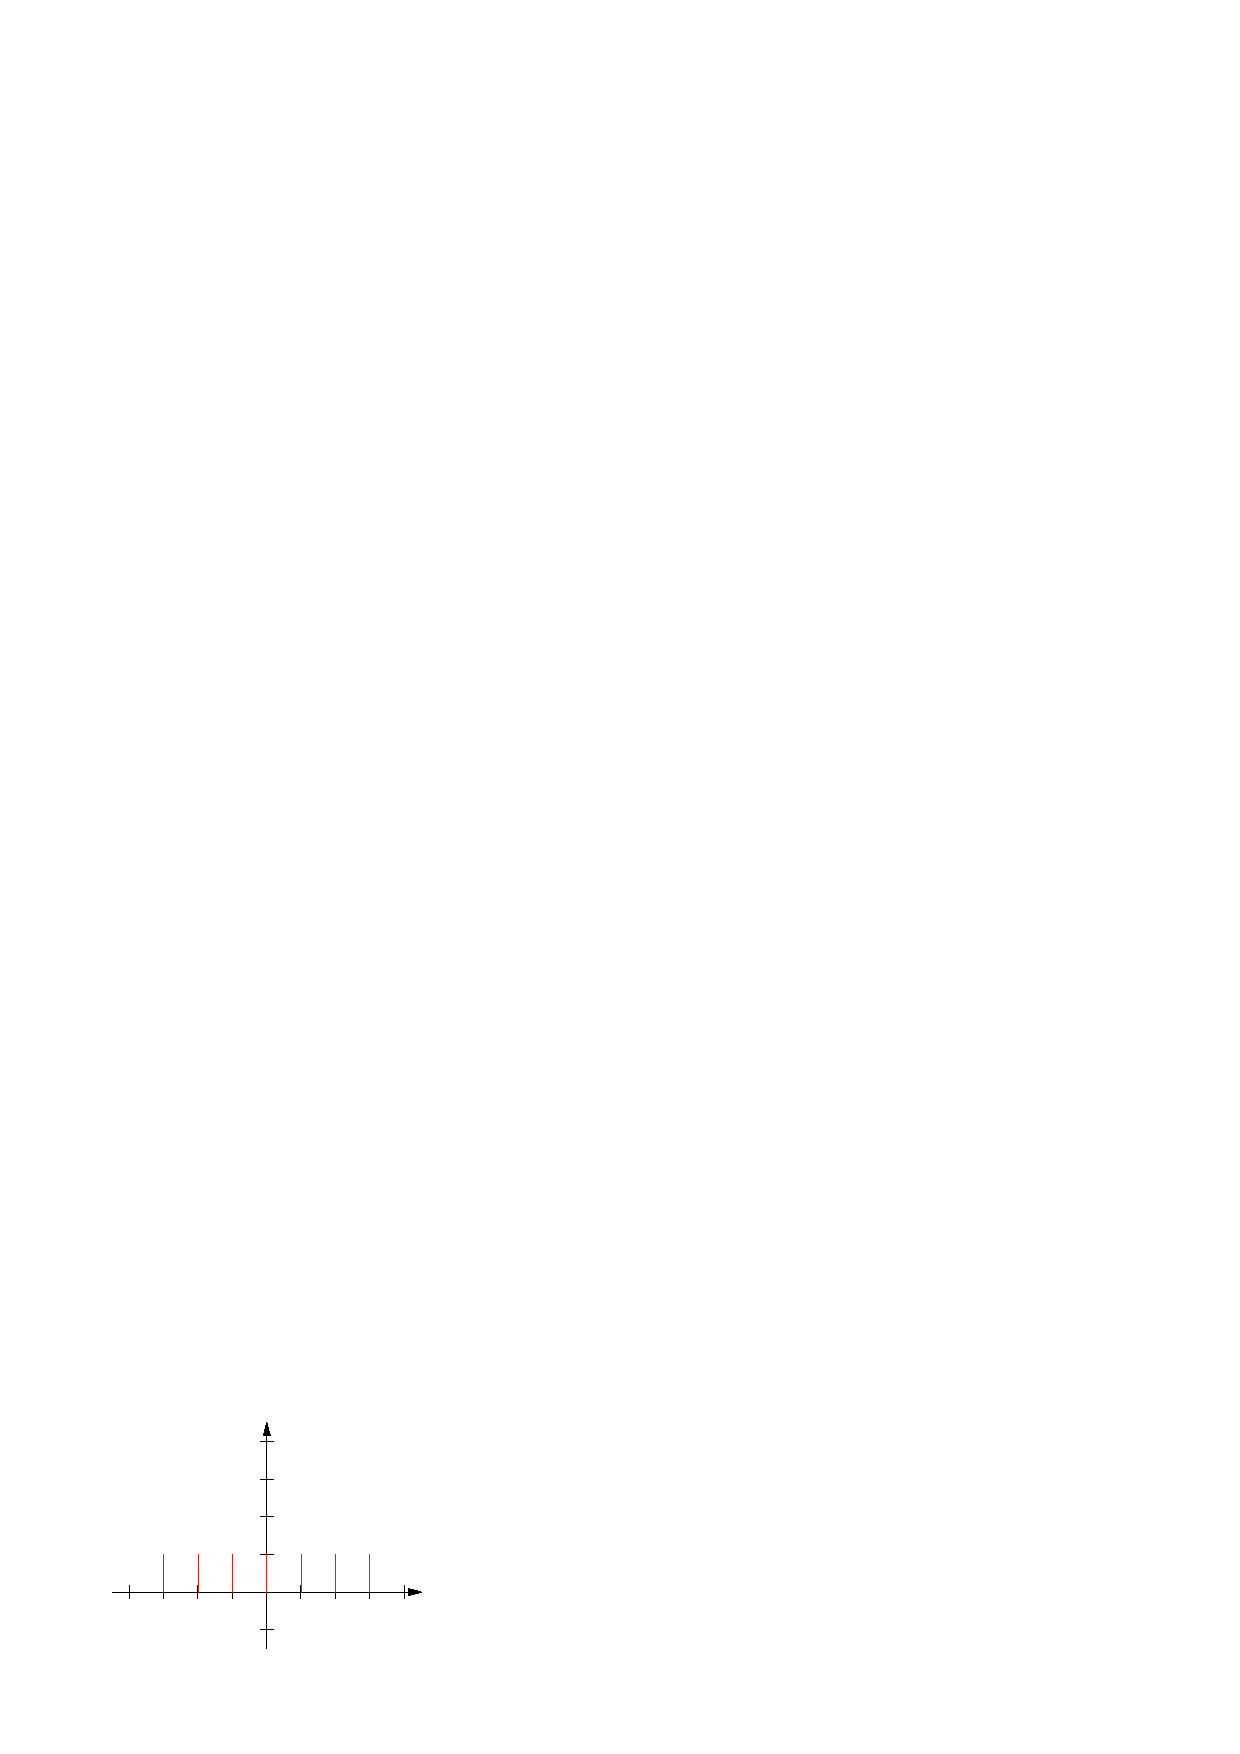
\includegraphics[width={158.40bp},height={108.00bp}]{figura_03_21}}%
    \gplfronttext
  \end{picture}%
\endgroup

        \captionsetup{labelformat=empty}
        \caption{Espectro de fase o argumento}
    \end{minipage}
\end{figure}

\section{Teorema de la multiplicación}
Dadas dos funciones periódicas con el mismo periodo $T$: $f_1(t)$ y $f_2(t)$.

Donde: $c_1n$ y $c_2n$, son los respectivos coeficientes complejos de
\emph{Fourier}.
\begin{equation}
    \frac{1}{T}\int_0^T\,f_1(t)f_2(t)\,dt
        =\sum_{n={-\infty}}^\infty\,c_1(n)\,c_2(-n)
        =\sum_{n={-\infty}}^\infty\,c_1(-n)\,c_2(n)
\end{equation}

\underline{Prueba}:

\begin{equation*}
\begin{split}
    \frac{1}{T}\int_0^T\,f_1(t)f_2(t)\,dt
        &=\frac{1}{T}\int_0^T\left[
            \sum_{n={-\infty}}^\infty\,c_1(n)\,e^{jn\omega_0\,t}
        \right]\,f_2(t)\,dt\\
        &=\sum_{n={-\infty}}^\infty\,c_1(n)\,\frac{1}{T}
            \int_0^T\,f_2(t)\,e^{jn\omega_0\,t}\,dt\\
        &=\sum_{n={-\infty}}^\infty\,c_1(n)c_2(-n)
\end{split}
\end{equation*}

\section{Teorema de \emph{Parseval}}
Sea: $f_1(t)=f_2(t)=f(t)$, con coeficientes de \emph{Fourier}:
$c_1(n)=c_2(n)=c_n$:

Partiendo del teorema de multiplicación:
\begin{equation*}
\begin{split}
    \frac{1}{T}\int_0^T\,f^2(t)\,dt
        &=\sum_{n={-\infty}}^\infty\,c_{(n)}\,c_{(-n)}\\
        &=\sum_{n={-\infty}}^\infty\,c_{(n)}\,c_{(n)}^*\\
        &=\sum_{n={-\infty}}^\infty\,{|c_n|}^2\\
        &=c_0^2+\sum_{\substack{n=-\infty\\n\neq0}}^\infty\,{|c_n|}^2\\
\end{split}
\end{equation*}
\begin{equation*}
    c_n=\frac{a_n-jb_n}{2}
\end{equation*}
\begin{equation*}
    {|c_n|}^2=\frac{a_n^2+b_n^2}{4}
\end{equation*}
\begin{equation*}
\begin{split}
    \frac{1}{T}\int_0^T\,f^2(t)\,dt
        &=c_0^2+\sum_{\substack{n=-\infty\\n\neq0}}^\infty
            \frac{a_n^2+b_n^2}{4}\\
        &=c_0^2+\frac{1}{4}\sum_{n=1}^\infty(a_n^2+b_n^2)
            +\frac{1}{4}\sum_{n=-1}^{-\infty}(a_n^2+b_n^2)\\
\end{split}
\end{equation*}

Cambiando $n$ por $-n$:
\begin{equation*}
\begin{split}
    \frac{1}{T}\int_0^T\,f^2(t)\,dt
        &=c_0^2+\frac{1}{4}\sum_{n=1}^\infty(a_n^2+b_n^2)
            +\frac{1}{4}\sum_{-n=-1}^{-\infty}(a_{(-n)}^2+b_{(-n)}^2)\\
\end{split}
\end{equation*}

Sabiendo que:
\begin{equation*}
    a_n^2=a_{(-n)}^2
\end{equation*}
\begin{equation*}
    {(-b_n)}^2=b_n^2
\end{equation*}
\begin{equation*}
\begin{split}
    \frac{1}{T}\int_0^T\,f^2(t)\,dt
        &=c_0^2+\frac{1}{4}\sum_{n=1}^\infty(a_n^2+b_n^2)
            +\frac{1}{4}\sum_{n=1}^\infty(a_n^2+b_n^2)\\
        &=c_0^2+\frac{1}{2}\sum_{n=1}^\infty(a_n^2+b_n^2)
\end{split}
\end{equation*}

\begin{equation}
    \frac{1}{T}\int_0^T\,f^2(t)\,dt
        =c_0^2+\frac{1}{2}\sum_{n=1}^\infty(a_n^2+b_n^2)
\end{equation}


\chapter{CONVECCIÓN NATURAL}

Es un mecanismo de transferencia de calor, propio de los medios fluidos y 
considerado como un fenómeno molecular.

\begin{figure}[!h]
\centering
\includegraphics[scale=1.40]{figura04_01.eps}
\end{figure}

Para el calculo del calor transferido se utiliza la ley de enfriamiento de
\emph{Newton}:
\begin{equation*}
    q_c = h\,A\,(t_s-t_\infty)
\end{equation*}

Donde:
\begin{itemize}
    \item $h$: Coeficiente de convección.
    \item $A$: Área de transferencia de calor.
    \item $t_s$: Temperatura de superficie.
    \item $t_\infty$: Temperatura del medio fluido.
\end{itemize}

\begin{equation*}
    q_c \neq 0 \Longrightarrow t_s-t_\infty \neq 0
\end{equation*}
\begin{equation*}
    q_c = 0 \Longrightarrow t_s = t_\infty
\end{equation*}
\begin{equation*}
    q_c \propto h
\end{equation*}

\section{Analogía de la película de convección con una pared}.
\begin{figure}[!h]
\centering
\includegraphics[scale=1.40]{figura04_02.eps}
\end{figure}

Transferencia de calor por conducción:
\begin{equation*}
    q = k\frac{A}{e_p}(t_s-t_\infty)=\frac{t_s-t_\infty}{e_p/k\,A}
\end{equation*}

Resistencia a la conducción:
\begin{equation*}
    R = \frac{e_p}{k\,A}
\end{equation*}

Transferencia de calor por convección:
\begin{equation*}
    q = h\,A(t_s-t_\infty)=\frac{t_s-t_\infty}{1/h\,A}
\end{equation*}

Resistencia a la convección:
\begin{equation*}
    R = \frac{1}{h\,A}
\end{equation*}

Igualando las resistencias:
\begin{equation*}
    \frac{e_p}{k\,A} = \frac{1}{h\,A}
\end{equation*}
\begin{equation*}
    h = \frac{e_p}{k}
\end{equation*}

$e_p$ es un parámetro variable y $k = f(t)$, por tanto:
\textbf{No es posible la analogía}.

\section{Método para la obtención de h}
Existen varios métodos:
\begin{itemize}
    \item Método analítico.
    \item Método empírico.
    \item Método por analogía.
    \item Método o análisis adimensional o análisis por grupos adimensional es.
\end{itemize}

Un \textbf{Grupo adimensional} es la agrupación de dos o mas magnitudes físicas
para obtener un grupo sin dimensiones.

Se consideran dos métodos para el calculo de grupos adimensionales:
\begin{itemize}
    \item Método algebraico.
    \item Método $\Pi$.
\end{itemize}

Una \textbf{magnitud física} es todo ente capaz de ser medido.

Una \textbf{unidad} es la asignación del valor unitario ($1$) a una magnitud
física.

\begin{table}[!h]
\begin{center}
\begin{tabular}{|>{\centering}m{2.4cm}<{\centering}
                |>{\centering}m{1.4cm}<{\centering}
                |>{\centering}m{1.4cm}<{\centering}
                |>{\centering}m{1.4cm}<{\centering}
                |>{\centering}m{1.4cm}<{\centering}
                |>{\centering}m{1.4cm}<{\centering}
                |>{\centering}m{1.4cm}<{\centering}|}
\hline
\textbf{Magnitud} &
\multicolumn{2}{c|}{\textbf{Sistema} \emph{Giorgi}} &
\multicolumn{2}{c|}{\textbf{Sistema técnico}} &
\multicolumn{2}{c|}{\textbf{Sistema ingenieril}} \tabularnewline \hline
&
\textbf{Métrica} &
\textbf{Ingles} &
\textbf{Métrica} &
\textbf{Ingles} &
\textbf{Métrica} &
\textbf{Ingles} \tabularnewline \hline
Masa & $kg$ & $lb$ & $utm$ & $slug$ & $kgm$ & $lbm$ \tabularnewline \hline
Fuerza & $N$ & $lb$ & $kgf$ & $lbf$ & $kgf$ & $lbf$ \tabularnewline \hline
Longitud & $m$ & $pie$ & $m$ & $pie$ & $m$ & $pie$ \tabularnewline \hline
Tiempo & $s$ & $s$ & $s$ & $s$ & $s$ & $s$ \tabularnewline \hline
Temperatura & $K$ & $R$ & $^{\circ}C$ & $^{\circ}F$ & $^{\circ}C$ & $^{\circ}F$
\tabularnewline \hline
\end{tabular}
\caption{Magnitudes en diversas unidades de medición.}
\end{center}
\end{table}

\textbf{\underline{Problema}}: Una esfera maciza se enfría en una corriente
fluida. Encontrar una expresión de grupos adimensionales para hallar de esta
expresión el valor de $h$.

\begin{figure}[!h]
\centering
\includegraphics[scale=1.40]{figura04_03.eps}
\end{figure}

\textbf{\underline{Pasos}}:
\begin{enumerate}
    \item Identificación de todas las magnitudes físicas que intervienen en el
        proceso.
        \begin{table}[!h]
        \begin{center}
        \begin{tabular}{|>{\centering}m{4.4cm}<{\centering}
                        |>{\centering}m{5.4cm}<{\centering}|}
        \hline
        \textbf{Esfera} & \textbf{Fluido} \tabularnewline \hline
        \hline
        Diámetro & Velocidad \tabularnewline \hline
        Material & Temperatura \tabularnewline \hline
        Temperatura & Densidad \tabularnewline \hline
        Acabado superficial & Calor especifico \tabularnewline \hline
        & Viscosidad \tabularnewline \hline
        & Coeficiente de conducción \tabularnewline \hline
        \end{tabular}
        \end{center}
        \end{table}
    \item Selección de las magnitudes físicas mas importantes.
        Pueden usarse:
        \begin{itemize}
            \item Analisis experimental.
            \item Analisis de varianza.
        \end{itemize}
        \begin{enumerate}
            \item Diámetro de la esfera ($D$).
            \item Diferencia de temperaturas ($\Delta{t}$).
            \item Velocidad del fluido ($v$).
            \item Densidad ($\rho$).
            \item Viscosidad ($\mu$).
            \item Calor especifico ($C_p$).
            \item Coeficiente de conducción ($k$).
            \item Coeficiente de convección ($h$).
        \end{enumerate}
    \item Expresar las magnitudes físicas elegidas con sus unidades.
        \begin{equation*}
        \def\arraystretch{1.5}
        \begin{array}{@{}cl@{}}
        \toprule
        \text{Magnitud} & \\
        \cmidrule(l){1-2}
        D & [m] \\
        \Delta{t} & [K] \\
        v & [m/s] \\
        \rho & [kg/m^3] \\
        \mu & [kg/m\,s] \\
        C_p & \dfrac{kcal}{kg\,^{\circ}C}
              \dfrac{kgf\,m}{kcal}
              \dfrac{N}{kgf}
              \dfrac{kg\frac{m}{s^2}}{N}
        =\dfrac{kg\,m^2}{kg\,^{\circ}C\,s^2}
        =\left[\dfrac{m^2}{s^2\,K}\right]\\
        k & \dfrac{kcal}{m\,h\,^{\circ}C}
            \dfrac{kg\frac{m^2}{s^2}}{kcal}
        =\dfrac{kg\,m^2}{m\,h\,^{\circ}C\,s^2}
        =\left[\dfrac{kg\,m}{s^3\,K}\right]\\
        h & \dfrac{kcal}{m^2\,h\,^{\circ}C}
            \dfrac{kg\frac{m^2}{s^2}}{kcal}
        =\dfrac{kg\,m^2}{m^2\,h\,^{\circ}C\,s^2}
        =\left[\dfrac{kg}{s^3\,K}\right]\\
        \bottomrule
        \end{array}
        \end{equation*}
\end{enumerate}

\subsection{Método algebraico}
\begin{enumerate}
    \setcounter{enumi}{3}
    \item Aplicar el método algebraico.
        \begin{equation*}
            h = f(D^a,\Delta{t}^b,v^c,\rho^d,\mu^e,C_p^f,k^g)+
                f^{'}(
                    D^{a_1},\Delta{t}^{b_1},v^{c_1},
                    \rho^{d_1},\mu^{e_1},C_p^{f_1},k^{g_1}
                )+
                \cdots
        \end{equation*}
        \begin{equation}
            h = f(D^a,\Delta{t}^b,v^c,\rho^d,\mu^e,C_p^f,k^g)
            \label{algebraico}
        \end{equation}
    \item Reemplazar en cada magnitud de la ecuación sus unidades
        correspondientes.
        \begin{equation*}
            \frac{kg}{s^3\,K} = f\left(
                [m]^a,[K]^b,\left[\frac{m}{s}\right]^c,
                \left[\frac{kg}{m^3}\right]^d,\left[\frac{kg}{m\,s}\right]^e,
                \left[\frac{m^2}{s^2\,K}\right]^f,
                \left[\frac{kg\,m}{s^3\,K}\right]^g\right)
        \end{equation*}
    \item Construir un sistema de ecuaciones lineales para cada exponente.
        \begin{equation}
            \begin{cases}
                [m] & 0 = a + c - 3d - e + 2f + g \\
                [kg] & 1 = d + e +g \\
                [s] & -3 = -c - e - 2f -3g \\
                [K] & -1 = b - f - g \\
            \end{cases}
        \end{equation}
    \item Expresar algunos exponentes en función de otros.
        \begin{equation*}
        \def\arraystretch{1.5}
        \begin{array}{@{}cc@{}}
        \toprule
        \text{Variable} & \text{Frecuencia} \\
        \cmidrule(l){1-2}
        a & 1 \\
        b & 1 \\
        c & 2 \\
        d & 2 \\
        e & 3 \\
        f & 3 \\
        g & 4 \\
        \bottomrule
        \end{array}
        \end{equation*}

        \begin{equation*}
            \begin{split}
            a
                &= -c + 3d + e - 2f - g \\
                &= -(3 - e - 2f - 3g) + 3(1 - e - g) + e - 2f - g \\
                &= -3 + e + 2f + 3g + 3 - 3e - 3g + e - 2f - g \\
                &= -e - g \\
            \end{split}
        \end{equation*}
        \begin{equation*}
            b = f + g - 1
        \end{equation*}
        \begin{equation*}
            c = 3 -e - 2f - 3g
        \end{equation*}
        \begin{equation*}
            d = 1 - e -g
        \end{equation*}
    \item Reemplazar en la ecuación (\ref{algebraico}) y resolver para los
        exponentes.
        \begin{equation*}
            h = f(
                D^{-e-g},
                \Delta{t}^{f+g-1},
                v^{-e-2f-3g+3},
                \rho^{-e-g+1},
                \mu^e,C_p^f,k^g
            )
        \end{equation*}
        \begin{equation*}
            h = f\left(
                \left[\frac{\mu}{D\,v\,\rho}\right]^e,
                \left[\frac{\Delta{t}\,C_p}{v^2}\right]^f,
                \left[\frac{\Delta{t}\,k}{D\,v^3\,\rho}\right]^g,
                \frac{v^3\,\rho}{\Delta{t}}
            \right)
        \end{equation*}
        \begin{equation*}
            \frac{h\,\Delta{t}}{v^3\,\rho} = f\left(
                \left[\frac{\mu}{D\,v\,\rho}\right]^e,
                \left[\frac{\Delta{t}\,C_p}{v^2}\right]^f,
                \left[\frac{\Delta{t}\,k}{D\,v^3\,\rho}\right]^g
            \right)
        \end{equation*}
    \item Verificar.
        \begin{equation*}
            \frac{h\,\Delta{t}}{v^3\,\rho} =
            \dfrac{\left[\frac{kg}{s^3\,K}\right][K]}
            {\left[\frac{m}{s}\right]^3\,\left[\frac{kg}{m^3}\right]} = 1
        \end{equation*}
        \begin{equation*}
            \frac{\mu}{D\,v\,\rho} =
            \dfrac{\left[\frac{kg}{m\,s}\right]}
            {[m]\left[\frac{m}{s}\right]\left[\frac{kg}{m^3}\right]} = 1
        \end{equation*}
        \begin{equation*}
            \frac{\Delta{t}\,C_p}{v^2} =
            \dfrac{[K]\left[\frac{m^2}{s^2\,K}\right]}
            {\left[\frac{m}{s}\right]^2} = 1
        \end{equation*}
        \begin{equation*}
            \frac{\Delta{t}\,k}{D\,v^3\,\rho} =
            \dfrac{[K]\left[\frac{kg\,m}{s^3\,K}\right]}
            {[m]\left[\frac{m}{s}\right]^3\left[\frac{kg}{m^3}\right]} = 1
        \end{equation*}
\end{enumerate}

Quedan por determinar:
\begin{itemize}
    \item Función $f$.
    \item Exponentes $e$, $f$, $g$.
    \item Relación entre grupos adimensionales.
\end{itemize}

Cuya solución se realiza en una fase experimental.

\subsection{Método $\Pi$}
\begin{enumerate}
    \setcounter{enumi}{3}
    \item Aplicar el método $\Pi$.
        \begin{equation}
            f(D,\Delta{t},v,\rho,\mu,C_p,k,h) = 0
            \label{pi}
        \end{equation}
        De estas magnitudes físicas se eligen las mas sencillas y las unidades
        del sistema internacional (SI) se expresan en función de las magnitudes
        elegidas.

        \begin{equation*}
            \begin{cases}
                [m] & D \\
                [kg] & \rho = \left[\frac{kg}{m^3}\right]
                    \rightarrow \rho\,D^3 \\
                [s] & v = \left[\frac{m}{s}\right] \rightarrow \dfrac{D}{v} \\
                [K] & \Delta{t}
            \end{cases}
        \end{equation*}

        \begin{equation*}
            \begin{split}
                N_T 
                    &= \text{\# de magnitudes físicas}
                     - \text{\# de magnitudes elegidas} \\
                    &= 8 - 4 \\
                    &= 4
            \end{split}
        \end{equation*}

        \underline{$\Pi_1$}:\\
        \begin{equation*}
            \mu = \left[\frac{kg}{m\,s}\right]
        \end{equation*}
        \begin{equation*}
            \Pi_1 = \mu\,\frac{m\,s}{kg}
                = \frac{\mu\,D\,\frac{D}{v}}{\rho\,D^3}
                = \frac{\mu}{\rho\,v\,D}
        \end{equation*}

        \underline{$\Pi_2$}:\\
        \begin{equation*}
            C_p = \left[\frac{m^2}{s^2\,K}\right]
        \end{equation*}
        \begin{equation*}
            \Pi_2 = C_p\,\frac{s^2\,K}{m^2}
                = \frac{C_p\,\frac{D^2}{v^2}\,\Delta{t}}{D^2}
                = \frac{C_p\,\Delta{t}}{v^2}
        \end{equation*}

        \underline{$\Pi_3$}:\\
        \begin{equation*}
            k = \left[\frac{kg\,m}{s^3\,K}\right]
        \end{equation*}
        \begin{equation*}
            \Pi_3 = k\,\frac{s^3\,K}{kg\,m}
                = \frac{k\,\frac{D^3}{v^3}\,\Delta{t}}{\rho\,D^3\,D}
                = \frac{k\,\Delta{t}}{\rho\,D\,v^3}
        \end{equation*}

        \underline{$\Pi_4$}:\\
        \begin{equation*}
            h = \left[\frac{kg}{s^3\,K}\right]
        \end{equation*}
        \begin{equation*}
            \Pi_4 = h\frac{s^3\,K}{kg}
            = \frac{h\,\frac{D^3}{v^3}\,\Delta{t}}{\rho\,D^3}
            = \frac{h\,\Delta{t}}{\rho\,v^3}
        \end{equation*}

        La ecuación (\ref{pi}), puede reescribirse como:
        \begin{equation}
            f(\Pi_1,\Pi_2,\Pi_3,\Pi_4) = 0
        \end{equation}
\end{enumerate}

\subsection{Tabla de grupos adimensionales conocidos}
\begin{equation*}
\def\arraystretch{1.5}
\begin{array}{@{}lccc@{}}
\toprule
\text{Nombre} & \text{Símbolo} & \text{Expresión} & \text{Uso} \\
\cmidrule(l){1-4}
\text{Número de \emph{Biot}} & [Bi] &
\dfrac{h}{k}\,L & \text{Conducción} \\
\text{Numero de \emph{Fourier}} & [Fo] &
\dfrac{\alpha}{L^2}\,\theta & \text{Conducción} \\
\text{Número de \emph{Nusselt}} & [Nu] &
h\,\dfrac{D}{k} & \text{Convección natural} \\
\text{Número de \emph{Prandtl}} & [Pr] &
C_p\,\dfrac{\mu}{k} & \text{Convección natural} \\
\text{Número de \emph{Grashof}} & [Gr] &
\left(g\dfrac{D^3}{v^2}\right)(\beta\,\Delta{t}) & \text{Convección natural} \\
\text{Número de \emph{Rayleigh}} & [Ra] &
Pr Gr & \text{Convección forzada} \\
\text{Número de \emph{Reynolds}} & [Re] &
\dfrac{\rho\,v\,D}{\mu} & \text{Convección forzada} \\
\text{Número de \emph{Mach}} & [Ma] & \dfrac{v}{v_s} & \\
\text{Número de \emph{Stanton}} & [St] & & \\
\text{Número de \emph{Péclet}} & [Pe] & & \\
\bottomrule
\end{array}
\end{equation*}

\subsection{Reglas para el manejo de grupos adimensionales}
\begin{itemize}
    \item El producto de dos o mas grupos adimensionales da como resultado otro
        grupo adimensional.
    \item La división entre grupos adimensionales da como resultado otro grupo
        adimensional.
        \begin{equation*}
            \frac{1}{\Pi_1} = \frac{\rho\,v\,D}{\mu} = \text{Re}
        \end{equation*}
        \begin{equation*}
            \frac{\Pi_4}{\Pi_3}
                = \dfrac{\frac{h\,\Delta{t}}{\rho\,v^3}}
                    {\frac{k\,\Delta{t}}{\rho\,D\,v^3}}
                = \frac{h\,D}{k}
                = \text{Nu}
        \end{equation*}
        \begin{equation*}
            \frac{\Pi_2\,\Pi_1}{\Pi_3}
                = \dfrac{\frac{C_p\,\Delta{t}}{v^2}\frac{\mu}{\rho\,v\,D}}
                    {\frac{k\,\Delta{t}}{\rho\,D\,v^3}}
                = \frac{C_p\,\mu}{k}
                = \text{Pr}
        \end{equation*}
\end{itemize}

\section{Ecuaciones recomendadas para $h$}

\textbf{Ecuaciones de \emph{Rice}}:

Si $\text{Gr} > 3$:
\begin{equation}
    \text{Nu}_f = 0.47\,(\text{Gr}_f\,\text{Pr}_f)^{0.25}
    \qquad\text{Tubos horizontales}
\end{equation}
\begin{equation}
    \text{Nu}_f = 0.59\,(\text{Gr}_f\,\text{Pr}_f)^{0.25}
    \qquad\text{Tubos verticales}
\end{equation}

Si $\text{Gr} < 3$: Debe usarse la siguiente gráfica:
\begin{figure}[!h]
\centering
\includegraphics[scale=0.40]{figura04_04.eps}
\end{figure}

El subíndice-índice $f$ (film) refiere a la película de convección natural.

\underline{Propiedades}:\\
\begin{figure}[!h]
\centering
\includegraphics[scale=1.40]{figura04_05.eps}
\end{figure}

\begin{equation}
    \text{Pr} = C_p\,\frac{\mu}{k}
\end{equation}
\begin{equation}
    \text{Gr} = \frac{g\,D^3\,\beta\,\Delta t}{\gamma^2}
\end{equation}
Donde:
\begin{itemize}
    \item $g$: Gravedad local ($9.78 [m/s]$).
    \item $\beta$: Coeficiente de dilatación volumétrico ($[^\circ C^{-1}]$).
    \item $\Delta t$: $t_s - t_\infty$.
    \item $\gamma$: Viscosidad cinemática ($[m^2/s]$).
    \item $D$: Longitud característica.
        \begin{itemize}
            \item Para tubos horizontales: $D=D_E$ (Diámetro externo).
            \item Para tubos verticales: $D=L$ (Altura).
        \end{itemize}
\end{itemize}

\begin{equation}
    \text{Nu} = \frac{h\,D}{k}
\end{equation}
Donde:
\begin{itemize}
    \item $D$: Longitud característica.
        \begin{itemize}
            \item Para ambos tubos: $D=D_E$ (Diámetro externo).
        \end{itemize}
\end{itemize}

\begin{equation}
    t_f (\text{temperatura de película}) = \frac{t_s+t_\infty}{2}
\end{equation}

\subsection{Caso: aire (flujo laminar)}
\begin{figure}[!h]
\centering
\includegraphics[scale=1.44]{figura04_06.eps}
\end{figure}

\begin{equation}
    h = 2.1\,\Delta t^{0.25}\qquad\text{Paredes horizontales hacia arriba}
\end{equation}
\begin{equation}
    h = 1.1\,\Delta t^{0.25}\qquad\text{Paredes horizontales hacia abajo}
\end{equation}
\begin{equation}
    h = 1.5\,\Delta t^{0.25}\qquad\text{Paredes verticales } L > 0.40
\end{equation}
\begin{equation}
    h = 1.2\,\left(\frac{\Delta t}{L}\right)^{0.25}
    \qquad\text{Paredes verticales } L < 0.40
\end{equation}
\begin{equation}
    h = 1.1\,\left(\frac{\Delta t}{D}\right)^{0.25}
    \qquad\text{Tubos horizontales y verticales}
\end{equation}

\subsection{Caso: Cualquier otro fluido, flujo turbulento, o cualquier forma
geométrica}
\begin{equation}
    \text{Nu} = C\,Ra^a
\end{equation}

Donde:
\begin{itemize}
    \item $C$, $a$, se extraen de la tabla $8-3$ del libro ``Transferencia de
        Calor'', de \emph{Pitts}.
\end{itemize}

\section{Convección en régimen transitorio}
Cuando el medio fluido es demasiado grande, su temperatura ($t_\infty$) no
tiende a permanecer constante, por tanto $h$ y $q_c$ también son constantes.
Esto se denomina ``convección en régimen permanente''.

Cuando el medio tiene su temperatura no constante ($t_\infty = f(\theta)$, tanto
su $h$ como su $q$ son variables. Esto se denomina ``convección en régimen no
permanente'' o ``convección en régimen transitorio''.

\subsection{Deducción de $t = f(\theta)$}
Se debe realizar un balance:

\begin{equation*}
    q_p\,\text{calor perdido por convección natural} = 
    q_s\,\text{calor sensible ganado por el fluido}
\end{equation*}
\begin{equation*}
    -q_c = q_s
\end{equation*}
\begin{equation*}
    -h\,A\,(t_s-t) = m\,C_p\,\frac{dt}{d\theta}
\end{equation*}
\begin{equation*}
    -\frac{dt}{t_s-t_\infty}\,\frac{C_p}{h} = \frac{A}{m}\,d\theta
\end{equation*}
\begin{equation*}
    -\frac{\bar{C_p}}{\bar{h}}\,\int_{t_i}^{t_f}\frac{dt}{t_s-t} =
        \frac{A}{m}\,\int_0^{\theta}\,d\theta
\end{equation*}
\begin{equation*}
    -\frac{\bar{C_p}}{\bar{h}}\,\ln\left(\frac{t_s-f_f}{t_s-t_i}\right) =
        \frac{A}{m}\,\theta
\end{equation*}
\begin{equation}
    \theta =
    -\frac{m\,\bar{C_p}}{A\,\bar{h}}\,\ln\left(\frac{t_s-f_f}{t_s-t_i}\right)
\end{equation}

\subsection{Casos particulares}

Para múltiples tubos horizontales y/o verticales el área total es la suma de las
áreas de cada tubo.

\begin{equation*}
    A_T = N_t A_t
\end{equation*}
\begin{equation*}
    A_t = \pi D_E\,l
\end{equation*}

En placas verticales se debe tomar el volumen por encima de la placa vertical.

\section{Cavidades}
\begin{figure}[!h]
\centering
\includegraphics[scale=2.00]{figura04_07.eps}
\end{figure}

\underline{Condición}:
\begin{equation*}
    \frac{L}{b} > 3
\end{equation*}
\\

Se hallan las propiedades del aire a la temperatura promedio:
\begin{equation*}
    \bar{t} = \frac{T_1 + T_2}{2}
\end{equation*}
\\

Y el calculo del número de \emph{Grashof} se hace con el espesor de la cavidad
como longitud característica.
\\
\begin{equation*}
    \text{Gr} = \frac{g\,b^3\,\beta\,(T_1 - T_2)}{\gamma^2}
\end{equation*}

\begin{figure}[!h]
\centering
\includegraphics[scale=0.32]{figura04_08.eps}
\end{figure}

Se tienen los siguientes casos:
\begin{table}[!h]
\begin{center}
\begin{tabular}{|>{\centering}m{3.8cm}<{\centering}
                |>{\centering}m{4.4cm}<{\centering}
                |>{\centering}m{4.4cm}<{\centering}|}
\hline
\textbf{Mecanismo} &
\textbf{Condición} &
\tabularnewline \hline
Conducción pura &
$\text{Gr} < 2000$ &
$\text{Nu} = 1$ \tabularnewline \hline
Convección natural en régimen laminar &
$\num{2e4} < \text{Gr} < \num{2e5}$ &
$\text{Nu} = 0.18\,\text{Gr}^{\frac{1}{4}}\,
\left(\frac{L}{b}\right)^{-\frac{1}{9}}$
\tabularnewline \hline
Convección natural en régimen turbulento &
$\num{2e5} < \text{Gr} < \num{2e7}$ &
$\text{Nu} = 0.065\,\text{Gr}^{\frac{1}{3}}\,
\left(\frac{L}{b}\right)^{-\frac{1}{9}}$
\tabularnewline \hline
\end{tabular}
\end{center}
\end{table}


\chapter{CONVECCIÓN FORZADA}

\begin{figure}[!h]
\centering
\includegraphics[scale=1.90]{figura05_01.eps}
\end{figure}

\begin{table}[!h]
\begin{center}
\begin{tabular}{|m{6.8cm}
                |m{6.8cm}|}
\hline
\textbf{Ventajas} &
\textbf{Desventajas} \tabularnewline \hline
Disminución del tiempo de proceso. &
Inversión en equipamiento. \tabularnewline \hline
Permite el manejo de grandes volúmenes. &
Gasto de energía para un sistema mecánico. \tabularnewline \hline
Transmisión de elevadas tasas de calor. &
Gasto de mantenimiento. \tabularnewline \hline
Uso industrial. & \tabularnewline \hline
\end{tabular}
\end{center}
\end{table}

\begin{equation*}
    q = h_{CF}\,A\,\Delta t
\end{equation*}

Donde $h_{CF}$, es el coeficiente de convección forzada, que es mayor al
coeficiente de convección natural.
\begin{equation*}
    h_{CF} > h_{CN}
\end{equation*}

\section{Calculo de $h$}
\underline{Casos}:
\begin{enumerate}
    \item Tubos únicos.
    \begin{enumerate}
        \item Flujo por el interior.
        \item Flujo por el exterior.
    \end{enumerate}
    \item Conjunto de tubos.
    \begin{enumerate}
        \item Método de \emph{Crimson} (Coeficiente externo).
    \end{enumerate}
\end{enumerate}

\underline{Tipos de régimen}:
\begin{itemize}
    \item Régimen laminar.
    \item Régimen turbulento.
\end{itemize}

\underline{Número de \emph{Reynolds}}:
\begin{equation}
    \text{Re} = \frac{v\,D\,\rho}{\mu}
\end{equation}

\section{Caso: Interior de tubos}
\begin{equation*}
    \rho = \frac{m}{V}
\end{equation*}
\begin{equation*}
    m = V\,\rho
\end{equation*}
\begin{equation*}
    \dot{m} = v\,A_T\,\rho
\end{equation*}
\begin{equation*}
    v\,\rho = \frac{\dot{m}}{A_T} = G
\end{equation*}

\begin{equation}
    \text{Re} = \frac{G\,D_I}{\mu}
\end{equation}

Donde:
\begin{itemize}
    \item $D_I$: Diámetro interno (Longitud característica).
    \item $A_T$: Sección transversal del tubo.
    \item $G$: Flujo másico por sección transversal.
\end{itemize}

Si:
\begin{itemize}
    \item $\text{Re} \le 2100$, el régimen es \textbf{laminar}.
    \item $\text{Re} > 2100$, el régimen es \textbf{turbulento}.
\end{itemize}

\subsection{Caso: Tubo único, flujo interior, régimen turbulento}
Se utiliza las ecuaciones de \emph{Dittus}-\emph{Boelter}:

\begin{equation}
    \text{Nu}_F = 0.023\,\text{Re}^{0.8}\,\text{Pr}^{0.33}
    \label{dittus1}
\end{equation}
\begin{equation}
    \text{Nu} = 0.023\,\text{Re}^{0.8}\,\text{Pr}^{0.4}
    \quad\text{(Calentamiento)}
    \label{dittus2}
\end{equation}
\begin{equation}
    \text{Nu} = 0.023\,\text{Re}^{0.8}\,\text{Pr}^{0.3}
    \quad\text{(Enfriamiento)}
    \label{dittus3}
\end{equation}

\begin{figure}[!h]
\centering
\includegraphics[scale=2.00]{figura05_02.eps}
\caption{Sección de un tubo.}
\end{figure}

Para (\ref{dittus1}), las propiedades se calculan a la temperatura de película:
\begin{equation*}
    t_\text{F} = \frac{t_\text{INT} + \bar{t}_{\infty}}{2}
\end{equation*}

Para (\ref{dittus2}) y (\ref{dittus3}), las propiedades se calculan a la
temperatura media del fluido:
\begin{equation*}
    \bar{t}_\infty = \frac{t_1 + t_2}{2}
\end{equation*}

Donde:
\begin{itemize}
    \item $t_\text{INT}$: Temperatura de la superficie interna.
    \item $\bar{t}_\infty$: Temperatura media o global del fluido.
\end{itemize}

\subsubsection{Caso: Gases}
$\text{Pr} = 0.74$ es un valor constante.
\begin{equation}
    \text{Nu} = 0.021\,\text{Re}^{0.8}
\end{equation}

\subsubsection{Caso: Flujo isotérmico (vapor)}
\begin{equation}
    h = 0.023\,
    \left(\frac{G^{0.8}}{D^{0.2}}\right)
    \left(\frac{Cp^{0.4}\,k^{0.6}}{\mu^{0.4}}\right)
\end{equation}

\subsubsection{Caso: Fluido muy viscoso ($\text{Re} \le 8000$)}
Se usa la ecuación de \emph{Sieder} y \emph{Tate}:
\begin{equation}
    \text{Nu} = 0.027\,\text{Re}^{0.8}\,\text{Pr}^{0.333}\,
    \left(\frac{\mu}{\mu_S}\right)^{0.14}
\end{equation}

Donde:
\begin{itemize}
    \item $\mu$: Viscosidad a la temperatura media del fluido.
    \item $\mu_S$: Viscosidad a la temperatura de superficie.
\end{itemize}

\subsection{Caso: Tubo único, flujo interior, régimen laminar}
La ecuación general es:

\begin{equation}
    \text{Nu} = 2.0\,
    \left(\frac{W\,Cp}{k\,L}\right)^{\frac{1}{3}}
    \left(\frac{\mu}{\mu_S}\right)^{0.14}
\end{equation}

Donde:
\begin{itemize}
    \item $W$: Flujo másico $[kg/h]$.
    \item $L$: Longitud del tubo $[m]$.
\end{itemize}

\subsubsection{Caso: Agua}
En este caso $\mu$ es constante, por tanto:

\begin{equation*}
    \frac{\mu}{\mu_S} = 1.0
\end{equation*}

\section{Caso: Flujo por el exterior de tubos}

\subsection{Caso: Régimen turbulento}
Para líquidos:
\begin{equation}
    \text{Nu}_\text{F} = \text{Pr}_\text{F}^{0.3}\,
    (0.35+0.47\text{Re}_\text{F}^{0.52})
\end{equation}

Para gases:
\begin{equation}
    \text{Nu}_\text{F} = 0.26\,\text{Pr}_\text{F}^{0.3}\,
    \text{Re}_\text{F}^{0.6}
\end{equation}

Las propiedades se calculan a la temperatura de película:
\begin{equation*}
    t_\text{F} = \frac{t_\text{WE} + \bar{t}_{\infty}}{2}
\end{equation*}
\begin{equation*}
    \bar{t}_\infty = \frac{t_i + t_o}{2}
\end{equation*}

\subsubsection{Caso: Aire y gases diatómicos}
\begin{equation}
    \text{Nu} = 0.32 + 0.43\,\text{Re}^{0.52}
\end{equation}
\begin{equation*}
    \text{Nu} = 0.45 + 0.33\,\text{Re}^{0.56}
\end{equation*}
\begin{equation*}
    \text{Nu} = 0.24\,\text{Re}^{0.6}
\end{equation*}

\subsubsection{Caso: Cambiadores de calor de doble tubo o tubos concéntricos}
\begin{figure}[!h]
\centering
\includegraphics[scale=2.00]{figura05_03.eps}
\caption{Sección de dos tubos concéntricos.}
\end{figure}

Se utiliza la ecuación de \emph{Davis}:
\begin{equation}
    \frac{h}{Cp\,G} = 0.029\,
    \left(\frac{D_\text{I}\,G}{\mu}\right)^{-0.2}
    \left(\frac{C_p\,\mu}{k}\right)^{-\frac{2}{3}}
    \left(\frac{\mu}{\mu_s}\right)^{0.14}
    \left(\frac{D_\text{E}}{D_\text{I}}\right)^{0.25}
\end{equation}
\begin{equation*}
    \frac{h}{Cp\,G} = 0.029\,
    \text{Re}^{-0.2}\,
    \text{Pr}^{-\frac{2}{3}}
    \left(\frac{\mu}{\mu_s}\right)^{0.14}
    \left(\frac{D_\text{E}}{D_\text{I}}\right)^{0.25}
\end{equation*}

Donde:
\begin{itemize}
    \item $D_\text{I}$: Diámetro interno de la zona anular.
    \item $D_\text{E}$: Diámetro externo de la zona anular.
\end{itemize}

Si, alguno de los tubos tiene un diámetro variable, se debe usar el valor del
perímetro, de la siguiente manera:
\begin{equation*}
    P = \pi\,D_\text{I}
\end{equation*}
\begin{equation*}
    D_\text{I} = \frac{P}{\pi}
\end{equation*}

Por ejemplo para un tubo cuadrado seria:
\begin{equation*}
    D_\text{I} = \frac{4\,l}{\pi}
\end{equation*}

\subsection{Caso: Régimen laminar}

\subsubsection{Caso: Líquidos ($0.1 < \text{Re} < 200$)}
\begin{equation}
    \text{Nu}_\text{F} = 0.86\,\text{Pr}_\text{F}^{0.3}\,
    \text{Re}_\text{F}^{0.43}
\end{equation}

\subsubsection{Caso: Líquidos ($\text{Re} > 200$) y
Gases ($0.1 < \text{Re} < 1000$)}
\begin{equation}
    \text{Nu}_\text{F} = \text{Pr}_\text{F}^{0.3}\,
    (0.35 + 0.47\,\text{Re}_\text{F}^{0.52})
\end{equation}

\subsubsection{Caso: Aire}
\begin{equation}
    \text{Nu}_\text{F} = 0.24\,\text{Re}^{0.6}
\end{equation}

\section{Caso: Flujo por el exterior de haces de tubos}
Se consideran dos tipos de arreglos:

\begin{enumerate}
    \item En linea o cuadrangular.
    \item Escalonado, triangular o al tres bolillo.
\end{enumerate}

\begin{figure}[!h]
\centering
    \begin{minipage}{.4\textwidth}
        \centering
        \includegraphics[scale=1.00]{figura05_04.eps}
        \caption{Arreglo en linea}
    \end{minipage}
    \begin{minipage}{.4\textwidth}
        \centering
        \includegraphics[scale=1.00]{figura05_05.eps}
        \caption{Arreglo escalonado}
    \end{minipage}
\end{figure}

\subsection{Método de \emph{Crimson}}
\begin{equation}
    \text{Nu} = C\,\text{Re}_\text{max}^n
\end{equation}

Donde:
\begin{itemize}
    \item $C$, $n$, se extraen de la tabla $7-7$ del libro ``Transferencia de
        Calor'', de \emph{Pitts}.
\end{itemize}

\begin{equation}
    \text{Re}_\text{max} = \frac{v_\text{max}\,D_E}{\nu}
\end{equation}

Donde:
\begin{itemize}
    \item $v_\text{max}$: Velocidad máxima en el pasaje mínimo $[m/s]$.
    \item $D_E$: Diámetro externo $[m]$.
    \item $\nu$: Viscosidad cinemática $[m^2/s]$.
\end{itemize}

Para un arreglo en linea, se tiene:
\begin{figure}[!h]
\centering
\includegraphics[scale=2.00]{figura05_06.eps}
\end{figure}

\begin{equation}
    P_\text{min} = a - D
\end{equation}
\begin{equation}
    v_\text{max} = \frac{V_\infty\,a}{a - D}
\end{equation}

Para un arreglo escalonado, se tiene:
\begin{figure}[!h]
\centering
\includegraphics[scale=2.00]{figura05_07.eps}
\end{figure}

\begin{equation}
    P_\text{min1} = \frac{a - D}{2}
\end{equation}
\begin{equation}
    P_\text{min2} = \sqrt{\left(\frac{a}{2}\right)^2 + b^2} - D
\end{equation}
\begin{equation}
    v_\text{max} = \frac{V_\infty\,(a/2)}{\text{min}(P_\text{min1}, P_\text{min2})}
\end{equation}

Para 10 o mas tubos se obtiene el coeficiente de convección en dirección de la
corriente:
\begin{equation*}
    h_o = \frac{\text{Nu}\,k}{D}
\end{equation*}

Para menos de 10 tubos en la dirección de la corriente, se debe corregir con el
factor que se encuentra en la tabla $7-8$ del libro ``Transferencia de
Calor'', de \emph{Pitts}.


%\chapter{CAMBIADORES DE CALOR}

\section{Concepto}
Es un equipo térmico en el que un fluido o medio mas ``caliente'' entrega calor
al fluido o medio mas ``frío''.

\section{Objetivos}
\begin{itemize}
    \item Optimización del uso de la energía mediante el aprovechamiento de la
        energía de desecho.
    \item Mejorar el control del proceso de transferencia de calor.
    \item Manejo de grandes cantidades de calor.
\end{itemize}

\section{Tipos de cambiadores}
\begin{itemize}
    \item Cambiador de contacto directo.
    \item Cambiador de contacto de superficie.
    \item Regeneradores.
\end{itemize}

\subsection{Cambiador de contacto directo (CD)}

% grafica ccd

\textbf{Ventajas}
\begin{itemize}
    \item Diseño, calculo y construcción relativamente fáciles.
    \item Costo bajo.
\end{itemize}

\textbf{Desventajas}
\begin{itemize}
    \item Solo intervienen fluidos de la misma naturaleza.
    \item Fluidos con diferentes grados de fuerza, composición, etc.
\end{itemize}

% grafica aplicaciones

\subsection{Cambiador de contacto de superficie (CS)}

% grafica ccs

\textbf{Ventajas}
\begin{itemize}
    \item Interviene cualquier tipo de fluido.
    \item Mayor control de los fluidos participantes.
    \item Aplicaciones industriales.
    \item Manejo de grandes tasas de calor.
\end{itemize}

\textbf{Desventajas}
\begin{itemize}
    \item Calculo y diseño complejos.
    \item Materiales y construcción caros.
    \item Costos de mantenimiento elevados.
\end{itemize}

%\subsection{Regeneradores}
% grafica regenerador

% grafica aplicacion

\section{Cambiadores de contacto de superficie}

\subsection{Cambiador de superficies planas o de flujo transversal}

% grafica ft

\textbf{Ventajas}
\begin{itemize}
    \item Calculo y diseño no complejo.
    \item Materiales y construcción relativamente económicos.
\end{itemize}

\textbf{Desventajas}
\begin{itemize}
    \item Presiones bajas a medias.
    \item Áreas de transferencia de calor limitadas.
\end{itemize}

\subsection{Cambiador de horquillas o de tubos concéntricos}

% grafica tc

\textbf{Ventajas}
\begin{itemize}
    \item Diseño y calculo relativamente fácil.
    \item Materiales y construcción económicos.
\end{itemize}

\textbf{Desventajas}
\begin{itemize}
    \item Área de transferencia de calor reducida.
    \item Gran probabilidad de fugas.
    \item Elevados costos de mantenimiento.
\end{itemize}

\subsection{Cambiador de superficies extendidas}
El objetivo es disminuir las dimensiones del cambiador de calor.

% grafica se

\textbf{Ventajas}
\begin{itemize}
    \item Permite disminuir notablemente las dimensiones del equipo.
\end{itemize}

\textbf{Desventajas}
\begin{itemize}
    \item Diseño y calculo muy complejos.
    \item Material caro adquirido de fabrica.
    \item Mantenimiento caro.
\end{itemize}

\subsection{Cambiador de calor de coraza y tubos}

% grafica cyt

\textbf{Ventajas}
\begin{itemize}
    \item Medianas a elevadas áreas de transferencia de calor.
    \item Permite el manejo de elevadas tasas de calor.
    \item Mayor control del proceso.
    \item Aplicación industrial.
\end{itemize}

\textbf{Desventajas}
\begin{itemize}
    \item Calculo y diseño complicado.
    \item Materiales y fabricación caros.
    \item Mantenimiento caro.
\end{itemize}

\section{Diseño y calculo de cambiadores de calor}

\subsection{Áreas involucradas}
\begin{itemize}
    \item Área térmica.
    \item Área fluida.
    \item Área de materiales.
    \item Área de fabricación.
    \item Área de mantenimiento y operación.
    \item Área económica.
\end{itemize}

\section{Calculo y diseño térmico de un cambiador}

El balance de calor en condiciones adiabáticas, el calor perdido por el fluido
caliente debe ser igual al calor ganado por el fluido frío.

\begin{equation}
    q_h = q_c
\end{equation}

Existen dos tipos de calor a considerarse:

\begin{itemize}
    \item Calor sensible ($q_s$).
    \item Calor latente ($q_l$).
\end{itemize}

\begin{equation*}
    -q_{sh} = q_{sc}
\end{equation*}
\begin{equation}
    -\dot{m}_h\,C_{ph}\,(t_{ho} - t_{hi}) = \dot{m}_c\,C_{pc}\,(t_{co} - t_{ci})
\end{equation}

\begin{equation*}
    -q_{lh} = q_{sc}
\end{equation*}
\begin{equation}
    -\dot{m}_h\,(-\Delta H) = \dot{m}_c\,C_{pc}\,(t_{co} - t_{ci})
\end{equation}

Donde:
\begin{itemize}
    \item $\dot{m}_h$, $\dot{m}_c$: Flujos másicos del fluido caliente y frío
        respectivamente.
    \item $C_{ph}$, $C_{pc}$: Calor especifico de los fluidos caliente y frío
        respectivamente.
    \item $t_{hi}$, $t_{ci}$: Temperaturas de entrada de los fluidos caliente y 
        frío respectivamente.
    \item $t_{ho}$, $t_{co}$: Temperaturas de salida de los fluidos caliente y 
        frío respectivamente.
    \item $\Delta H$: Calor de condensación del fluido caliente.
\end{itemize}

% grafica de cambio de fase

Los objetivos de balance pueden ser:
\begin{itemize}
    \item Obtener el calor.
    \item Obtener un dato flotante.
\end{itemize}

\underline{Ecuación del calor transmitido en el cambiador de calor}:

\begin{equation}
    q = U\,A\,\Delta t
\end{equation}

Donde:
\begin{itemize}
    \item $q$: Calor transmitido.
    \item $U$: Coeficiente global de transferencia de calor.
    \item $A$: Área de transferencia de calor.
    \item $\Delta t$: Diferencia de temperaturas en el cambiador de calor.
\end{itemize}

\begin{equation*}
    -q_h = q_c = q
\end{equation*}
\begin{equation}
    A = \frac{q}{U\,\Delta t}
\end{equation}

\section{Coeficiente global}

\subsection{Pared vertical}

% grafica u pared

\begin{equation*}
    q = \frac{t_i - t_o}{R_{ci} + R_p + R_{co}}
\end{equation*}
\begin{equation*}
    q = \dfrac{t_i - t_o}{\frac{1}{h_i\,A_i} + \frac{\Delta x_p}{k_p\,A_p} + \frac{1}{h_o\,A_o}}
\end{equation*}
\begin{equation*}
    A_i = A_p = A_o = A
\end{equation*}
\begin{equation*}
    q = \dfrac{A\,(t_i - t_o)}{\frac{1}{h_i} + \frac{\Delta x_p}{k_p} + \frac{1}{h_o}}
\end{equation*}

\begin{equation}
    U = \dfrac{1}{\frac{1}{h_i} + \frac{\Delta x_p}{k_p} + \frac{1}{h_o}}
\end{equation}

\subsection{Conductor cilíndrico}

% grafica u cilindrico

\begin{equation*}
    q = \frac{\bar{t}_o - \bar{t}_i}{R_{co} + R_p + R_{ci}}
\end{equation*}
\begin{equation*}
    q = \dfrac{\bar{t}_o - \bar{t}_i}{\frac{1}{h_o\,A_o} + \frac{\Delta r_p}{k_p\,A_p} + \frac{1}{h_i\,A_i}}
\end{equation*}
\begin{equation*}
    A_o \neq A_p \neq A_i
\end{equation*}

Multiplicando por $A_o/A_o$:
\begin{equation*}
    q = \dfrac{A_o(\bar{t}_o - \bar{t}_i)}{\frac{1}{h_o} + \frac{A_o\,\Delta r_p}{k_p\,A_p} + \frac{A_o}{h_i\,A_i}}
\end{equation*}

Considerando:
\begin{equation*}
    A_o = \pi\,D_e\,l
\end{equation*}
\begin{equation*}
    A_i = \pi\,D_i\,l
\end{equation*}
\begin{equation*}
    \frac{A_o}{A_i} = \frac{D_e}{D_i}
\end{equation*}

\begin{equation*}
    \frac{A_o\,\Delta r_p}{A_p} = \frac{\pi\,D_e\,l\,\Delta r_p}{\frac{A_o-A_i}{\ln(\frac{A_o}{A_i})}}
\end{equation*}

\begin{equation*}
    \begin{split}
        A_o - A_i
            &= \pi\,D_e\,l - \pi\,D_i\,l\\
            &= \pi\,l\,(D_e - \,D_i)\\
            &= \pi\,l\,(2r_o - 2r_i)\\
            &= 2\pi\,l\,(r_o - r_i)\\
            &= 2\pi\,l\,\Delta r_p\\
    \end{split}
\end{equation*}

\begin{equation*}
    \begin{split}
        \frac{A_o\,\Delta r_p}{A_p}
            &= \frac{\pi\,D_e\,l\,\Delta r_p}{\frac{2\pi\,l\Delta r_p}{\ln(\frac{A_o}{A_i})}}\\
            &= \frac{D_e}{2}\ln\left(\frac{D_e}{D_i}\right)\\
    \end{split}
\end{equation*}

Por tanto:

\begin{equation*}
    q = \dfrac{A_o(\bar{t}_o - \bar{t}_i)}{\frac{1}{h_o} + \frac{D_e}{2k_p}\ln\left(\frac{D_e}{D_i}\right) + \frac{D_e}{h_i\,D_i}}
\end{equation*}
\begin{equation*}
    q = U_o\,A_o\,\Delta t
\end{equation*}

$U_o$: Coeficiente global referido a la superficie externa.
\begin{equation}
    U_o = \dfrac{1}{\frac{1}{h_o} + \frac{D_e}{2k_p}\ln\left(\frac{D_e}{D_i}\right) + \frac{1}{h_i}\left(\frac{D_e}{D_i}\right)}
\end{equation}

Multiplicando por $A_i/A_i$:
\begin{equation*}
    q = \dfrac{A_i(\bar{t}_o - \bar{t}_i)}{\frac{A_i}{h_o\,A_o} + \frac{A_i\,\Delta r_p}{k_p\,A_p} + \frac{1}{h_i}}
\end{equation*}

Considerando:
\begin{equation*}
    \begin{split}
    \frac{A_i\,\Delta r_p}{A_p}
        &= \frac{\pi\,D_i\,l\,\Delta r_p}{\frac{A_o-A_i}{\ln(\frac{A_o}{A_i})}}\\
            &= \frac{\pi\,D_i\,l\,\Delta r_p}{\frac{2\pi\,l\Delta r_p}{\ln(\frac{A_o}{A_i})}}\\
            &= \frac{D_i}{2}\ln\left(\frac{D_e}{D_i}\right)\\
    \end{split}
\end{equation*}

Por tanto:

\begin{equation*}
    q = \dfrac{A_i(\bar{t}_o - \bar{t}_i)}{\frac{1}{h_i} + \frac{D_i}{2k_p}\ln\left(\frac{D_e}{D_i}\right) + \frac{D_i}{h_o\,D_e}}
\end{equation*}
\begin{equation*}
    q = U_i\,A_i\,\Delta t
\end{equation*}

$U_i$: Coeficiente global referido a la superficie interna.
\begin{equation}
    U_i = \dfrac{1}{\frac{1}{h_i} + \frac{D_i}{2k_p}\ln\left(\frac{D_e}{D_i}\right) + \frac{1}{h_o}\left(\frac{D_i}{D_e}\right)}
\end{equation}

Igualando las expresiones:
\begin{equation*}
    U_o\,A_o\,\Delta t = U_i\,A_i\,\Delta t
\end{equation*}

\begin{equation}
    \frac{U_o}{U_i} = \frac{A_i}{A_o} = \frac{D_i}{D_e}
\end{equation}

\section{Incrustaciones, costras, o ensuciamiento}

% grafica incrustaciones

\begin{equation*}
    q = \frac{\Delta t}{R_{ci} + R_{di} + R_p + R_{do} + R_{co}}
\end{equation*}
\begin{equation*}
    \frac{1}{U_d} = \frac{1}{U} + \sum R_d
\end{equation*}
\begin{equation*}
    \sum R_d = R_{di} + R_{do}
\end{equation*}

\begin{equation}
    \frac{1}{U_{do}} = \frac{1}{U_o} + \sum R_d
\end{equation}
\begin{equation}
    \frac{1}{U_{di}} = \frac{1}{U_i} + \sum R_d
\end{equation}

Donde:
\begin{itemize}
    \item $U_d$: Coeficiente de diseño (con incrustaciones).
    \item $U$: Coeficiente limpio (sin incrustaciones).
\end{itemize}

\begin{equation}
    q = U_d\,A_d\,\Delta t = U_{do}\,A_{do}\,\Delta t = U_{di}\,A_{di}\,\Delta t
\end{equation}

\section{Disposiciones de los fluidos en un cambiador}
Pueden ser:

\begin{itemize}
    \item En contracorriente o contra flujo.
    \item En corriente paralela.
    \item Con cambio de fase.
\end{itemize}

% grafica cambiadores

\subsection{Calculo del gradiente}
El gradiente de temperatura se puede aproximar por medio de:
\begin{equation*}
    \Delta t = \frac{1}{2}\,(\Delta t_1 + \Delta t_2)
\end{equation*}

Para el calculo del valor exacto se procede de la siguiente manera:

% grafica gradiente

\begin{equation*}
    dq = U\,\Delta t\,dA
\end{equation*}

Del gráfico puede verse que:
\begin{equation*}
    \frac{d\Delta t}{dq} = \frac{\Delta t_1 - \Delta t_2}{q}
\end{equation*}

Combinando ambas expresiones:
\begin{equation*}
    \frac{d\Delta t}{U\,\Delta t\,dA} = \frac{\Delta t_1 - \Delta t_2}{q}
\end{equation*}
\begin{equation*}
    \frac{d\Delta t}{U\,\Delta t} = \frac{\Delta t_1 - \Delta t_2}{q}\,dA
\end{equation*}

Se simplifica la expresión considerando que $U$ es constante y no esta en
función de la gradiente de temperatura.
\begin{equation*}
    \int\frac{d\Delta t}{U\,\Delta t} = \int\frac{\Delta t_1 - \Delta t_2}{q}\,dA
\end{equation*}
\begin{equation*}
    \frac{1}{U}\,\ln\left(\frac{\Delta t_1}{\Delta t_2}\right) = \frac{\Delta t_1 - \Delta t_2}{q}\,A
\end{equation*}
\begin{equation*}
    q = U\,A\,\frac{\Delta t_1 - \Delta t_2}{\ln\left(\frac{\Delta t_1}{\Delta t_2}\right)}
\end{equation*}

Por tanto el gradiente logarítmico es:
\begin{equation}
    \Delta t_{log} = \frac{\Delta t_1 - \Delta t_2}{\ln\left(\frac{\Delta t_1}{\Delta t_2}\right)}
\end{equation}

\subsection{Pasos del cambiador}

% grafico cambiadores

\subsection{Factor de corrección ($F_c$)}

\begin{equation*}
    \Delta t = F_c\,\Delta t_{log}
\end{equation*}

Donde:
\begin{itemize}
    \item $\Delta_{log}$ para un cambiador 1:1 en contracorriente.
\end{itemize}

Para cambiadores 1:1 y condensadores el factor de corrección $F_c = 1$.

Para hallar el factor de corrección se usa la tabla de corrección usando los
valores $X$ y $Z$:

\begin{equation}
    X = \frac{t_{c2} - t_{c1}}{t_{h1} - t_{c1}}
\end{equation}
\begin{equation}
    Z = \frac{t_{h1} - t_{h2}}{t_{c2} - t_{c1}}
\end{equation}

\subsection{Eficacia de un cambiador}

\begin{enumerate}
    \item $Z > 1$:
        \begin{equation}
            \eta = \frac{t_{c2} - t_{c1}}{t_{h2} - t_{c1}}
        \end{equation}
    \item $Z < 1$:
        \begin{equation}
            \eta = \frac{t_{h1} - t_{h2}}{t_{h1} - t_{c1}}
        \end{equation}
\end{enumerate}

\section{Calculo del numero de tubos ($N_T$)}

\subsection{Criterio de la transferencia de calor}

\begin{equation*}
    A_o = \pi\,D_e\,L_t
\end{equation*}
\begin{equation*}
    L_t = \frac{A_o}{\pi\,D_e}
\end{equation*}
\begin{equation*}
    N_T = \frac{L_t}{L}
\end{equation*}

Donde:
\begin{itemize}
    \item $L_t$: Longitud de tramo o longitud de $1$ tubo.
\end{itemize}

\subsection{Criterio del flujo másico}

\begin{equation*}
    N_T = \frac{\dot{m}}{\dot{m}_1}
\end{equation*}

Donde:
\begin{itemize}
    \item $\dot{m}$: Flujo másico total (fluido interno).
    \item $\dot{m}_1$: Flujo másico por $1$ tubo.
\end{itemize}

\begin{equation*}
    \dot{m} = v\,A_t\,\rho
\end{equation*}
\begin{equation*}
    \dot{m}_1 = v\,A_{t1}\,\rho
\end{equation*}
\begin{equation*}
    N_T = \frac{A_t}{A_{t1}}
\end{equation*}

\underline{Caso 1:1}:
\begin{equation*}
    N_T\Biggr|_q = N_T\Biggr|_{\dot{m}}
\end{equation*}

\underline{Caso 1:2}:
\begin{equation*}
    N_T\Biggr|_q = 2\,N_T\Biggr|_{\dot{m}}
\end{equation*}

\underline{Caso 1:3}:
\begin{equation*}
    N_T\Biggr|_q = 3\,N_T\Biggr|_{\dot{m}}
\end{equation*}

\section{Flujograma para el calculo de un cambiador de calor}

% grafica flujograma

\section{Ebullición}

% grafica ebullición

\begin{itemize}
    \item $I$: Convección libre.
    \item $II$: Formación de burbujas individuales.
    \item $III$: Formación de burbujas en columnas.
    \item $IV$: Película inestable.
    \item $V$: Película estable.
    \item $VI$: Radiación afecta la película.
\end{itemize}

\section{Condensación}
Es el proceso por el que vapor saturado se convierte en liquido, mediante la
extracción de calor latente.

% grafica condensación

Tipos de condensación:
\begin{enumerate}
    \item Condensación en forma de película.
    \item Condensación en forma de gotas.
\end{enumerate}

Depende de factores como: el tipo de valor o el tipo de superficie.

\begin{equation*}
    q = h_{\text{cond}}\,A\,(t_v - t_s)
\end{equation*}
\begin{equation*}
    q = \dot{m}_v\,(\Delta H)
\end{equation*}

Donde:
\begin{itemize}
    \item $h_{\text{cond}}$: Coeficiente de condensación $[kcal/m^2 h ^\circ C]$.
    \item $A$: Superficie de condensación $[m^2]$.
    \item $t_v$: Temperatura de vapor.
    \item $t_s$: Temperatura de superficie fría.
    \item $\dot{m}_v$: Flujo másico del condensado o del vapor $[kg/h]$.
    \item $\Delta H$: Calor de condensación $[kcal/kg]$.
\end{itemize}

\subsection{Calculo de $h$ de condensación}

\underline{Para superficies verticales}:

Para placas:
\begin{equation}
    h = 1.13\,\left(\frac{k_f^3\,\rho_f^2\,g\,\Delta H}{L\,\mu_f\,(t_v - t_s)}\right)^{\frac{1}{4}}
\end{equation}
Para tubos:
\begin{equation}
    h = 1.18\,\left(\frac{k_f^3\,\rho_f^2\,g\,\pi\,D}{\mu_f\,W}\right)^{\frac{1}{3}}
\end{equation}

\underline{Para tubos horizontales}:
\begin{equation}
    h = 0.725\,\left(\frac{k_f^3\,\rho_f^2\,g\,\Delta H}{N^{2/3}\,D\,\mu_f\,(t_v - t_s)}\right)^{\frac{1}{4}}
\end{equation}

Las propiedades del fluido se calculan a la temperatura media de la película
condensada:

\begin{equation}
    t_f = t_v - \frac{3}{4}\,(t_v - t_s)
\end{equation}

Donde:
\begin{itemize}
    \item $L$: Altura de la superficie.
    \item $D$: Diámetro externo.
    \item $W$: Flujo másico de condensado.
        \begin{equation*}
            W = \frac{\dot{m}_v}{N_T}
        \end{equation*}
    \item $N$: Numero de tubos por columna.
\end{itemize}

\subsection{Calculo de $A$}

\begin{equation*}
    q = h_{\text{cond}}\,A\,(t_v - t_s)
\end{equation*}
\begin{equation*}
    q = \dot{m}_v\,(\Delta H)
\end{equation*}

\begin{equation}
    A = \frac{\dot{m}_v\,(\Delta H)}{h_{\text{cond}}\,A\,(t_v - t_s)}
\end{equation}

\section{Método NUT (Numero de unidades térmicas)}
Su importancia radica en que no es necesario conocer las temperaturas de salida
de los fluidos.

\begin{equation}
    \epsilon = \frac{q_r}{q_{\text{max}}}
\end{equation}
\begin{equation*}
    q_{\text{max}} = C_{\text{min}}\,(t_{h1} - t_{c1})
\end{equation*}
\begin{equation*}
    C_{\text{min}} = \min(C_h, C_c)
\end{equation*}

\begin{equation*}
    C_h = \dot{m}_h\,C_{ph}
\end{equation*}
\begin{equation*}
    C_c = \dot{m}_c\,C_{pc}
\end{equation*}

Donde:
\begin{itemize}
    \item $q_r$: Calor real transmitido.
        \begin{equation*}
            q_r = -q_h = q_c
        \end{equation*}
    \item $q_{\text{max}}$: Calor máximo transmitido en un cambiador de calor
        1:1 de área infinita.
    \item $C$: Capacidad térmica.
        \begin{equation*}
            C = \dot{m}\,C_p
        \end{equation*}
\end{itemize}

\begin{equation}
    \text{NUT} = \frac{U\,A}{C_{\text{min}}}
\end{equation}

Físicamente en NUT nos da la idea del tamaño del cambiador.

\section{Superficies aletadas, aleteadas o extendidas}

% grafica aleta

\underline{Balance}:
\begin{equation*}
    q\Biggr|_x = q\Biggr|_{x+\Delta x} + q_c
\end{equation*}

Donde:
\begin{itemize}
    \item $q\Biggr|_x$: Calor que ingresa el VC.
    \item $q\Biggr|_{x+\Delta x}$: Calor que sale del VC.
    \item $q_c$: Calor que se transfiere por convección del VC al medio exterior.
    \item VC: Volumen de control.
\end{itemize}

\begin{equation*}
    q\Biggr|_x - q\Biggr|_{x+\Delta x} - q_c = 0
\end{equation*}
\begin{equation*}
    -k_x\,A(x)\,\frac{dt}{dx}\Biggr|_x - \left(-k_x\,A(x)\,\frac{dt}{dx}\Biggr|_{x + \Delta x}\right) - h\,S(x)\,(t-t_{\infty}) = 0
\end{equation*}
\begin{equation*}
    S(x) = P(x)\,A(x)
\end{equation*}
\begin{equation*}
    -k_x\,A(x)\,\frac{dt}{dx}\Biggr|_x + k_x\,A(x)\,\frac{dt}{dx}\Biggr|_{x + \Delta x} - h\,P(x)\,A(x)\,(t-t_{\infty}) = 0
\end{equation*}

\textbf{Ecuación general de una superficie extendida}:
\begin{equation}
    \frac{d}{dx}\left[k_x\,A(x)\,\frac{dt}{dx}\right] - h\,P(x)\,(t-t_{\infty}) = 0
\end{equation}

Donde:
\begin{itemize}
    \item $A(x)$: Área transversal de la aleta.
    \item $P(x)$: Perímetro de la aleta.
    \item $t$: Temperatura de la aleta.
    \item $t_{\infty}$: Temperatura del medio exterior.
    \item $h$: Coeficiente de convección de la aleta.
\end{itemize}

\subsection{Caso: Superficie con sección transversal uniformemente variable}

% grafica aleta1

\begin{equation}
    \frac{d}{dx}\left[\left[A_o + (A_L - A_o)\,\frac{x}{L}\right]\,\frac{dt}{dx}\right] - \frac{h}{k}\left[P_o + (P_L - P_o)\,\frac{x}{L}\right]\,(t - t_{\infty}) = 0
\end{equation}

Donde:
\begin{itemize}
    \item $A_o$: Área en la base.
    \item $P_o$: Perímetro en la base.
    \item $A_L$: Área en el extremo.
    \item $P_L$: Perímetro en el extremo.
\end{itemize}

\subsection{Caso: Aletas de sección transversal uniforme}

% grafica aleta2

\begin{equation}
    \frac{d^2 t}{dx^2} - \frac{h\,P}{k\,A}\,(t - t_{\infty}) = 0
\end{equation}

\subsection{Caso: Aletas circulares de espesor constante}

% grafica aleta3

\begin{equation*}
    \frac{d}{dr}\left(r\,\frac{dt}{dr}\right)-\frac{h\,r}{k\,t}\,(t-t_{\infty}) = 0
\end{equation*}

Soluciones para aletas de sección transversal constante:
\begin{equation*}
    \frac{d^2 t}{dx^2} - \frac{h\,P}{k\,A}\,(t - t_{\infty}) = 0
\end{equation*}
\begin{equation*}
    \theta = t - t_{\infty}
\end{equation*}
\begin{equation*}
    m^2 = \frac{h\,P}{k\,A}
\end{equation*}
\begin{equation}
    \frac{d^2 t}{dx^2} - m^2\,\theta = 0
\end{equation}

\underline{Solución general}:
\begin{equation*}
    \theta = C_1\,e^{mx} + C_2\,e^{-mx}
\end{equation*}
\begin{equation*}
    \theta = A\,\cosh(mx) + B\,\senh(mx)
\end{equation*}

\underline{Solución particular}:
Se debe resolver los coeficientes con las condiciones de contorno.

\begin{enumerate}
    \item \textbf{Aletas muy largas}:
        \begin{equation*}
            x = 0 \rightarrow \theta = \theta_0
        \end{equation*}
        \begin{equation*}
            x = \infty \rightarrow \theta = \theta
        \end{equation*}
        \begin{equation*}
            \frac{\theta}{\theta_0} = e^{-mx}
        \end{equation*}
        \begin{equation}
            \frac{t - t_{\infty}}{t_i - t_{\infty}} = e^{-mx}
        \end{equation}
    \item \textbf{Temperatura conducida en $x = L$}:
        \begin{equation*}
            x = 0 \rightarrow \theta = \theta_0
        \end{equation*}
        \begin{equation*}
            x = L \rightarrow \theta = \theta_L
        \end{equation*}
        \begin{equation*}
            \theta_L = t_L - t_{\infty}
        \end{equation*}
        \begin{equation*}
            \theta_0 = t_0 - t_{\infty}
        \end{equation*}
        \begin{equation*}
            \theta = t - t_{\infty}
        \end{equation*}
        \begin{equation}
            \frac{\theta}{\theta_0} = \frac{t - t_{\infty}}{t_0 - t_{\infty}} = \left(\frac{\theta_L}{\theta_0} - e^{-mL}\right)\left(\frac{e^{mx} - e^{-mx}}{e^{mL} - e^{-mL}}\right) + e^{-mx}
        \end{equation}
    \item \textbf{Extremo de la aleta aislado}:
        \begin{equation*}
            x = 0 \rightarrow \theta = \theta_0
        \end{equation*}
        \begin{equation*}
            x = L \rightarrow \frac{d\theta}{dx} = \theta_0
        \end{equation*}
        \begin{equation}
            \frac{\theta}{\theta_0} = \frac{t - t_{\infty}}{t_0 - t_{\infty}} = \frac{e^{mx}}{1 + e^{2mL}} + \frac{e^{-mx}}{1 + e^{-2mL}}
        \end{equation}
    \item \textbf{Conducción en el extremo es igual a la convección en el extremo}:
        \begin{equation*}
            x = 0 \rightarrow \theta = \theta_0
        \end{equation*}
        \begin{equation*}
            x = L \rightarrow k\,\frac{d\theta}{dx} = h\,\theta
        \end{equation*}
        \begin{equation}
            \frac{\theta}{\theta_0} = \dfrac{t - t_{\infty}}{t_0 - t_{\infty}} = \frac{\cosh(m(L-x))+(\frac{h}{m\,k})\senh(m(L-x))}{\cosh(mL)+(\frac{h}{m\,k})\senh(mL)}
        \end{equation}
\end{enumerate}

\subsection{Método de la eficiencia de aleta}

% grafica aleta4

\begin{equation}
    \frac{\theta}{\theta_0} = \dfrac{t - t_{\infty}}{t_0 - t_{\infty}} = \frac{I_o(n\,r)\,K(n\,r_0)+K_0(n\,r)\,I_1(n\,r_2)}{I_0(n\,r_1)\,K_1(n\,r_2)+K_0(n\,r)\,I_1(n\,r_2)}
\end{equation}
\begin{equation*}
    n = \sqrt{\frac{2h}{kr}}
\end{equation*}

Donde:
\begin{itemize}
    \item $I_o$: Ecuación de \emph{Bessel} modificada de primera especie.
    \item $K_1$: Ecuación de \emph{Bessel} modificada de segunda especie.
\end{itemize}

\underline{Balance}:
\begin{equation*}
    q_t = q_a + q_{s/a}
\end{equation*}
\begin{equation*}
    q_a = \eta_a\,h_a\,A_a\,(t - t_{\infty})
\end{equation*}
\begin{equation*}
    q_{s/a} = h_o\,A_{s/a}\,(t - t_{\infty})
\end{equation*}
\begin{equation*}
    q_t = \eta_a\,h_a\,A_a\,(t - t_{\infty}) + h_o\,A_{s/a}\,(t - t_{\infty})
\end{equation*}

\begin{equation*}
    A_{s/a} = N_a\,A_{s/a1}
\end{equation*}
\begin{equation*}
    A_{a} = N_a\,A_{a1}
\end{equation*}

\begin{equation*}
    q = N_a\,[h_o\,A_{s/a1}\,(t_o - t_{\infty} + \eta_a\,h_a\,A_{a1}\,(t - t_{\infty}]
\end{equation*}

Donde:
\begin{itemize}
    \item $N_a$: Numero de aletas.
    \item $A_{s/a1}$: Área libre entre dos aletas.
    \item $A_{a1}$: Área de una aleta.
\end{itemize}

\underline{Simplificación}:
\begin{equation*}
    h_o \approx h_a
\end{equation*}

\begin{equation*}
    q = N_a\,h_o\,(t_o - t_{\infty})(A_{s/a1} + \eta\,A_{a1})
\end{equation*}


%\chapter{Transformada inversa de \emph{Laplace}}

Si $\mathcal{L}\{f(t)\}=F(s)$:
\begin{equation}
    \mathcal{L}^{-1}\{F(s)\}=f(t)
\end{equation}

Definida para $t>0$.

La transformada inversa de \emph{Laplace} regresa del dominio de ``s'' al
dominio de ``t''.

\textbf{Ejemplo}:
\begin{equation*}
    \mathcal{L}^{-1}\biggl\{\frac{1}{s^n}\biggl\}
\end{equation*}
\begin{equation*}
    \mathcal{L}\{t^n\}=\frac{\Gamma(n+1)}{s^{n+1}}
\end{equation*}
\begin{equation*}
    t^n=\mathcal{L}^{-1}\biggl\{\frac{\Gamma(n+1)}{s^{n+1}}\biggl\}
\end{equation*}
\begin{equation*}
    \frac{t^n}{\Gamma(n+1)}=\mathcal{L}^{-1}\biggl\{\frac{1}{s^{n+1}}\biggl\}
\end{equation*}
\begin{equation}
    \mathcal{L}^{-1}\biggl\{\frac{1}{s^n}\biggl\}=\frac{t^{n-1}}{\Gamma(n)}
\end{equation}

En particular $n\in\mathbb{N}$:
\begin{equation}
    \mathcal{L}^{-1}\biggl\{\frac{1}{s^n}\biggl\}=\frac{t^{n-1}}{(n-1)!}
\end{equation}

\section{Tabla de transformadas de \emph{Laplace} inversas}

\begin{equation*}
\def\arraystretch{1.4}
\begin{array}{@{}cll@{}}
\toprule
 & F(s) & f(t)=\mathcal{L}^{-1}\{F(s)\};t>0\\
\cmidrule(l){1-3}
 1 & \dfrac{k}{s}
   & k\\
\cmidrule(l){1-3}
 2 & \dfrac{1}{s^n}
   & \dfrac{t^{n-1}}{\Gamma(n)};\quad\dfrac{t^{n-1}}{(n-1)!}\,n\in\mathbb{N}\\
\cmidrule(l){1-3}
 3 & \dfrac{1}{s-a}
   & e^{at}\\
\cmidrule(l){1-3}
 4 & \dfrac{1}{s^2+a^2}
   & \dfrac{1}{a}\sen(at)\\
\cmidrule(l){1-3}
 5 & \dfrac{s}{s^2+a^2}
   & \cos(at)\\
\cmidrule(l){1-3}
 6 & \dfrac{1}{s^2-a^2}
   & \dfrac{1}{a}\senh(at)\\
\cmidrule(l){1-3}
 7 & \dfrac{s}{s^2-a^2}
   & \cosh(at)\\
\cmidrule(l){1-3}
 8 & \arctan\left(\dfrac{a}{s}\right)
   & \dfrac{1}{t}\sen(at)\\
\cmidrule(l){1-3}
 9 & k
   & k\delta(t)\\
\cmidrule(l){1-3}
10 & e^{-as}
   & \delta(t-a)\\
\bottomrule
\end{array}
\end{equation*}

\section{Propiedades de la transformada inversa de \emph{Laplace}}

\subsection{Linealidad}
\begin{equation}
    \mathcal{L}^{-1}\{a_1\,F_1(s)+a_2\,F_2(s)\}
    =a_1\,f_1(t)+a_2\,f_2(t)
\end{equation}

\subsection{Desplazamiento en $t$}
Si $\mathcal{L}^{-1}\{F(s)\}=f(t)$:
\begin{equation}
    \mathcal{L}^{-1}\{F(s)\,e^{-as}\}=f(t-a)u(t-a)
\end{equation}

\subsection{Desplazamiento en $s$}
Si $\mathcal{L}^{-1}\{F(s)\}=f(t)$:
\begin{equation}
    \mathcal{L}^{-1}\{F(s-a)\}=f(t)\,e^{at}
\end{equation}

\subsection{División por $s$}
Si $\mathcal{L}^{-1}\{F(s)\}=f(t)$:
\begin{equation}
    \mathcal{L}^{-1}\biggl\{\frac{F(s)}{s}\biggl\}=\int_0^t\,f(t)\,dt
\end{equation}

En general:
\begin{equation}
    \mathcal{L}^{-1}\biggl\{\frac{F(s)}{s^n}\biggl\}
        =\int_0^t\int_0^t\dots\int_0^t\,f(t)\,dt\dots\,dt\,dt
\end{equation}

\subsection{Transformada inversa de la derivada}
Si $\mathcal{L}^{-1}\{F(s)\}=f(t)$:
\begin{equation}
    \mathcal{L}^{-1}\{F'(s)\}=-t\,f(t)
\end{equation}

En general:
\begin{equation}
    \mathcal{L}^{-1}\{F^{(n)}(s)\}={(-1)}^n\,t^n\,f(t)
\end{equation}

\section{Descomposición en fracciones parciales}
En la mayoría de los casos se tienen funciones racionales de la siguiente forma:

\begin{equation*}
    F(s)=\frac{P(s)}{Q(s)}
\end{equation*}

Donde el grado del numerador debe ser menor al grado del denominador. Para
hallar la transformada inversa se debe descomponer en fracciones parciales de
acuerdo a los factores del denominador. Se tienen los siguientes casos:

\subsection{Factores lineales no repetidos}
\begin{equation*}
    \frac{P(s)}{(s-a_1)(s-a_2)\dots(s-a_n)}
        =\frac{A_1}{s-a_1}+\frac{A_2}{s-a_2}+\cdots+\frac{A_n}{s-a_n}
\end{equation*}

\subsection{Factores lineales y repetidos}
\begin{equation*}
    \frac{P(s)}{{(s-a)}^m{(s-b)}^n}
        =\frac{A_1}{s-a}+\frac{A_2}{{(s-a)}^2}+\cdots+\frac{A_m}{{(s-a)}^m}
        +\frac{B_1}{(s-b)}+\frac{B_2}{{(s-a)}^2}+\cdots+\frac{B_n}{{(s-b)}^n}
\end{equation*}

\subsection{Factores cuadráticos (con raíces imaginarias o complejas)}
\begin{equation*}
    \frac{P(s)}{(s^2+{a_1}s+b_1)(s^2+{a_2}s+b_2)}
        =\frac{{A_1}s+B_1}{s^2+{a_1}s+b_1}
        +\frac{{A_2}s+B_2}{s^2+{a_2}s+b_2}
\end{equation*}

\section{Convolución}
\begin{equation*}
    f_1(t)*f_2(t)=\int_0^t\,f_1(\tau)f_2(t-\tau)\,d\tau
\end{equation*}
\begin{equation*}
\begin{split}
    \mathcal{L}\{f_1(t)*f_2(t)\}
        &=\int_0^{\infty}\left[\int_0^t\,f_1(\tau)f_2(t-\tau)\,d\tau\right]e^{-st}\,dt\\
        &=\int_{t=0}^{t=\infty}\int_{\tau=0}^{\tau=t}\,f_1(\tau)f_2(t-\tau)e^{-st}\,d\tau\,dt\\
        &=\lim_{M\rightarrow\infty}\int_{\tau=0}^{\tau=M}\int_{t=\tau}^{t=M}\,f_1(\tau)f_2(t-\tau)e^{-st}\,dt\,d\tau\\
        &=\lim_{M\rightarrow\infty}\int_0^M\,f_1(\tau)\,d\tau\int_{\tau}^{M}\,f_2(t-\tau)e^{-st}\,dt
\end{split}
\end{equation*}
\begin{equation*}
    u=t-\tau\rightarrow\,t=u+\tau
\end{equation*}
\begin{equation*}
    du=dt
\end{equation*}
\begin{equation*}
\begin{split}
    \mathcal{L}\{f_1(t)*f_2(t)\}
        &=\lim_{M\rightarrow\infty}\int_0^M\,f_1(\tau)\,d\tau\int_{0}^{M-\tau}\,f_2(u)e^{-s(u+\tau)}\,du\\
        &=\int_0^{\infty}\,f_1(\tau)e^{-st}\,d\tau\int_0^{\infty}\,f_2(u)e^{-su}\,du\\
        &=F_1(s)\,F_2(s)
\end{split}
\end{equation*}
\begin{equation}
    \mathcal{L}\{f_1(t)*f_2(t)\}=F_1(s)\,F_2(s)
\end{equation}


\section{Transformada inversa por convolución}
\begin{equation}
    \mathcal{L}^{-1}\{F_1(s)\,F_2(s)\}=f_1(t)*f_2(t)
\end{equation}

Donde:
\begin{equation*}
    f_1(t)=\mathcal{L}^{-1}\{F_1(s)\}
\end{equation*}
\begin{equation*}
    f_2(t)=\mathcal{L}^{-1}\{F_2(s)\}
\end{equation*}



\end{document}

